%%%%%%%%%%%%%%%%%%%%%%%%%%%%%%%%%%%%%%%%%%%%%%%%%%%%%%%%%%%%%%%%%%%%%%%%%%%%%%%%%%%%%%%%%
%%                                                                                     %%
%%                This file is part of the CAPH Compiler distribution                  %%
%%                            http:%/caph.univ-bpclermont.fr                           %%
%%                                                                                     %%
%%                                  Jocelyn SEROT                                      %%
%%                         Jocelyn.Serot@univ-bpclermont.fr                            %%
%%                                                                                     %%
%%         Copyright 2011-2018 Jocelyn SEROT.  All rights reserved.                    %%
%%  This file is distributed under the terms of the GNU Library General Public License %%
%%      with the special exception on linking described in file ..%LICENSE.            %%
%%                                                                                     %%
%%%%%%%%%%%%%%%%%%%%%%%%%%%%%%%%%%%%%%%%%%%%%%%%%%%%%%%%%%%%%%%%%%%%%%%%%%%%%%%%%%%%%%%%%

\documentclass[a4paper]{report}

\usepackage{amsmath,amssymb,stmaryrd,latexsym}
\usepackage{titlepic}
\usepackage{syntax}
\usepackage{alltt}
\usepackage{graphicx}   % Including Graphics
\usepackage{bcprules}   % Benjamin Pierce's Proof Rule Package
\usepackage{semabbrev} 
%\usepackage{verbatim} 
\usepackage{spverbatim}
\usepackage{alltt} 
\usepackage{xspace} 
\usepackage{listings} 
\usepackage{ifthen}
\usepackage{adjustbox}
\usepackage{xhfill}% http://ctan.org/pkg/xhfill
%\usepackage{color}
\usepackage[multiple]{footmisc}
\usepackage{algorithm}
\usepackage{algpseudocode}

\newboolean{devel}
\setboolean{devel}{false}

\lstloadlanguages{C++,VHDL}
\lstset{frameround=tttt} 
\lstset{captionpos=t}
\lstset{breaklines=true}
%\lstset{aboveskip=2\medskipamount}
%\lstset{belowskip=1.5\medskipamount}
%\lstset{abovecaptionskip=\medskipamount}
\lstdefinelanguage{Caph}{keywords={function,constant,actor,in,out,var,rules,stream,port,init,from,to,net,type,let,and,of,const,extern},morecomment=[l]{--}}
\lstset{language=Caph}
\lstset{frame=single}

%\renewcommand\lstlistingname{Example}

%%% Better hyphenation:
%\sloppy
\setlength{\topmargin}{0pt}
\setlength{\oddsidemargin}{0pt}
\setlength{\textheight}{600pt}
\setlength{\textwidth}{448pt}

%\Newcommand{\docdate}{\today} %%%!!!!

\newcommand{\version}{2.8}
%\ifthenelse{\boolean{devel}}{\newcommand{\version}{1.3}}{\newcommand{\version}{1.1}}
%% This has to be fixed !

\newcommand{\ie}{\emph{i.e.}\xspace}
\newcommand{\txt}[1]{\hbox{#1}}
\newcommand{\emtxt}[1]{\hbox{\em{#1}}}
\newcommand{\bftxt}[1]{\hbox{\bf{#1}}}
\ifthenelse{\boolean{devel}}{\newcommand{\note}[1]{\marginpar{\tiny #1}}}{\newcommand{\note}[1]{}}
\newcommand{\todo}[1]{\note{TODO: #1}}
\ifthenelse{\boolean{devel}}{\newcommand{\tbw}[1]{$\spadesuit$ {\bf To be written\ldots}\xspace}}{\newcommand{\tbw}[1]{}}
\ifthenelse{\boolean{devel}}{\newcommand{\tbc}[1]{$\spadesuit$ {\bf To be continued\ldots}\xspace}}{\newcommand{\tbc}[1]{}}

\newcommand{\caph}{CAPH\xspace}
\newcommand{\fgn}{{\sc fgn}\xspace}
\newcommand{\ocaml}{{\sc Objective Caml}\xspace}

\newenvironment{example}{\medskip\noindent{\it Example :}\begin{alltt}}{\end{alltt}}
%\newenvironment{caphexample}{\begin{lstlisting}}{\end{lstlisting}}

\algnewcommand\algorithmicforeach{\textbf{for each}}
\algdef{S}[FOR]{ForEach}[1]{\algorithmicforeach\ #1\ \algorithmicdo}


\title{CAPH Reference Manual - \version}

\author{J. S\'erot}%\footnote{Universit\'e Clermont Auvergne, Clermont-Ferrand, France; %\texttt{jocelyn.serot@uca.fr}}}

\titlepic{\includegraphics[width=0.5\textwidth]{figs/caph-logo}}
\date{}

\begin{document}

\maketitle

\tableofcontents

%%%%%%%%%%%%%%%%%%%%%%%%%%%%%%%%%%%%%%%%%%%%%%%%%%%%%%%%%%%%%%%%%%%%%%%%%%%%%%%%%%%%%%%%%
%%                                                                                     %%
%%                This file is part of the CAPH Compiler distribution                  %%
%%                            http:%/caph.univ-bpclermont.fr                           %%
%%                                                                                     %%
%%                                  Jocelyn SEROT                                      %%
%%                         Jocelyn.Serot@univ-bpclermont.fr                            %%
%%                                                                                     %%
%%         Copyright 2011-2018 Jocelyn SEROT.  All rights reserved.                    %%
%%  This file is distributed under the terms of the GNU Library General Public License %%
%%      with the special exception on linking described in file ..%LICENSE.            %%
%%                                                                                     %%
%%%%%%%%%%%%%%%%%%%%%%%%%%%%%%%%%%%%%%%%%%%%%%%%%%%%%%%%%%%%%%%%%%%%%%%%%%%%%%%%%%%%%%%%%

\chapter{Introduction}
\label{chap:intro}

This document describes the \caph programming language.  \caph\footnote{\caph stands for \emph{Caph
    just Ain't Plain HDL}. \emph{Caph} is also the name of the second bright star in the
  constellation of Cassiopeia.} is a domain-specific, high-level language for programming FPGAs.
\caph is based upon the \emph{dataflow process network} model of computation~\cite{DPN} and
produces implementations relying on a pure \emph{data-driven} execution model.  The \caph compiler
is able to generate synthetizable VHDL code from high-level descriptions of programs as networks of
interconnected dataflow actors.

\medskip This report is structured as follows: the remainder of this chapter provides motivation and
general background; Chapter~\ref{chap:overview} is an overview of the \caph language design,
including informal descriptions of the expression, network and actor sub-languages. The full
concrete syntax is given in chapter~\ref{chap:syntax} and the abstract syntax of the core language
in chapter~\ref{chap:abssyn}. Chapter~\ref{chap:typing} gives the formal typing rules for \caph
programs. Chapter~\ref{chap:static} gives the formal static semantics,
\emph{i.e.} the interpretation of \caph programs as \emph{data-flow graphs}.
Chapter~\ref{chap:dynamic-semantics} gives the formal dynamic semantics, which provides a way to
\emph{simulate} \caph programs.  Chapter~\ref{chap:interm-repr} describes
  the intermediate representation of \caph programs used as an input for the back-end code
  generators. Chapter~\ref{cha:using-caph-compiler} describes, pragmatically, how to use the
compiler in order to obtain graphical representations of programs, simulate them or invoke the
SystemC or VHDL backend in order to generate code. Chapter~\ref{cha:stdlib} gives the contents of
some ``standard libraries''. Chapter~\ref{cha:foreign-funct-interf} describes
the mechanism by which existing C or VHDL functions can be used by \caph
programs. Chapter~\ref{cha:compiler-options} is a summary of compiler options.
 Chapter~\ref{cha:variants-impl} is a short, technical, overview of how \emph{variant
  types} (described in chapter~\ref{chap:overview}) are implemented in SystemC and VHDL. 

\clearpage

\section{Motivation, goals and principles}

The design of the \caph language was guided by the following motivations and general principles:

\medskip \textbf{Specificity}. Although most of its underlying concepts are very general -- and
could indeed be applied to a large variety of programming languages targetting either software or
hardware --, the \caph language has been primarily designed to program FPGAs. This deliberate
orientation allowed us to make clear and argumented choices regarding the set of supported
features.
Other languages relying on the same model of computation (MoC) -- such as \textsc{cal}~\cite{CAL}
for example -- are less specific, targeting both software and hardware implementations, and
sometimes offer a richer set of features. But this richness comes at the price of ambiguity
since it's frequent that not all features are supported in hardware implementations. Moreover, the
set of supported features is not always clearly documented and must often be defined by tedious,
repeated experiments. Our approach is more pragmatic, if less ambitious: if it can be described, it
can be implemented.

\medskip
\textbf{Formal basis}. We strongly adhere to the idea that any decent programming language should be
based upon formal semantics, describing in a complete and unambiguous manner the meaning of
programs. The essentially \emph{functional} orientation of \caph greatly eases the
writing of such semantics. It also makes it possible to describe formally, and
in a platform-independant way, the transformation process by which the high level language source
code is turned into low-level VHDL code, a highly desirable property in our case, since it allows 
reasoning about this process (for certification and optimization purposes for example). Another
advantage is the ability to derive (in a systematic way) a reference interpreter for the
language. Such a reference interpreter can then be used latter to assess the correctness of the
results produced by generated low-level code.

\medskip
\textbf{Minimum distance} between the programming model and the execution model. This is the key
idea for being able to produce efficient low-level harware solutions from high-level descriptions
while keeping adherence to the second principle. Abstraction and efficiency being generaly
perceived as contradictory requirements, this principle is often interpreted as : keep the the
abstraction low at source level. Fortunately, this is not the case with the dataflow programming
and execution models \caph is relying on. A large part of this is due to the natural affinity
between the dataflow MoC and the concepts used in purely functional programming languages (absence
of side-effects, polymorphic type systems, higher-order constructs).

\medskip
Beside these general principals, \caph was also developped with a set of more technical / pragmatical
goals in mind :

\medskip
\textbf{Strict separation of concerns} between computation and communication. This is reflected by
the structure of the language, which embeds an
\emph{expression language} (for describing computations) within
a \emph{declaration language} (for describing the global structure of the program) on the one hand,
and provides two separate sub-languages for describing the behavior of actors and the communication
network by which these actors interact, on the other hand.

\medskip
\textbf{Composability, modularity}. This refers to the ability to build large, complex applications
from smaller, simpler ones. This is naturally supported by the dataflow model of computation (no
shared variables and hence no hidden dependencies) and the purely functional coordination language
(referential transparency).

\medskip
\textbf{Reuse}. Within the language, this is supported by \emph{higher-order} constructs. At the
actor level, higher-order actors can be used to encapsulate recurrent patterns of
\emph{computations}. At the network level, higher-order functions can be used to encapsulate recurrent patterns of
\emph{communication}. \caph also offers the ability to import legacy existing code (in VHDL for
synthesis, in C/SystemC for simulation).

\medskip
\textbf{Arbitrary data structuring}. By this we mean the ability to encode values -- and, jointly,
to describe actors operating on these values -- having an arbitrarily complex data structure.
In particular, the language should support the description of operations on 
non-regular and/or or variable-sized data structures (lists or trees, as opposed to fixed-sized
arrays, for instance). In other words, the target applications should not be limited to regular
signal or image processing. In \caph, this is provided by separating the tokens exchanged by actors
into two classes : \emph{data tokens} (carrying actual values) and \emph{control tokens} (acting as
structuring delimiters). 

\section{Language principles}
\label{sec:language-principles}

\caph is based upon the \emph{dataflow process network} model of computation~\cite{DPN}.
Applications are described networks of computational units, called \emph{actors}, exchanging
\emph{streams} of tokens through FIFO channels.
Interaction between actors is strictly limited to token exchange
through channels, so that the behavior of each actor can be completely described in terms of actions
performed on its inputs to produce outputs (no side effect, strictly local control).

We will illustrate this model with a very simple example, involving four basic actors. These actors
are depicted Fig.~\ref{fig:fouractors}. Actor \texttt{INC} (resp. \texttt{DEC}) adds
(resp. substracts) 1 to each element of its input stream. Actor \texttt{MUL} performs point-wise
multiplication of two streams. Actor \texttt{DUP} duplicates its input stream\footnote{In
  Fig.~\ref{fig:fouractors}, streams are denoted (ordered) from right to left; for example, the
  actor \texttt{ADD} first processes the token \texttt{1}, then the token \texttt{2}, \emph{etc.}
  Since streams are potentially infinite, their end is denoted ``\texttt{...}''. However, when describing
  actors \emph{textually}, streams will be denoted from left to right; for example:
  \texttt{ADD:1,2,... = 2,3,...}}. Now, if we connect
these four actors to build the network depicted in Fig~\ref{fig:networkfour}, this network computes
$f(x)=(x+1)\times(x-1)$ for each element $x$ of its input stream. I.e. if the input stream \emph{i}
is \texttt{1,2,3,...}, then the output stream \emph{o} will be \texttt{0,3,8,...}

\begin{figure}[h]
  \centering
  \includegraphics[width=1.0\textwidth]{figs/fouractors}
  \caption{Four basic actors}
  \label{fig:fouractors}
\end{figure}

\begin{figure}[h]
  \centering
  \includegraphics[width=0.75\textwidth]{figs/networkfour}
  \caption{A dataflow process network}
  \label{fig:networkfour}
\end{figure}

\medskip
Such a model of computation is indeed very general and can be interpreted in different ways, 
depending in particular in 
\begin{itemize}
\item the kind of behavior that can be assigned to actors (purely functional, stateful, firing
  semantics, \ldots),
\item the exact nature of channels (single place buffer / FIFO, bounded / unbounded, \ldots),
\item how networks are described.
\end{itemize}

In \caph
\begin{itemize}
\item the behavior of actors is specified using a set of \emph{transition rules} using \emph{pattern
    matching} and
  actors are stateful,
\item channels are bounded FIFOs,
\item networks are described in a \emph{implicit} manner, using a set of \emph{functional
    equations}.
\end{itemize}
These aspects are detailed in the next section.

\section{Language Structure}
\label{sec:language-structure}

In common with other coordination language approaches such as 
Hume~\cite{Hume}, \caph takes a layered approach (see Fig.~\ref{fig:languagestruct}).

\begin{figure}[h]
  \centering
  \includegraphics[width=0.75\textwidth]{figs/languagestruct}
  \caption{Caph language structure}
  \label{fig:languagestruct}
\end{figure}

The outermost (\emph{declaration}) layer declares types, global values (constant and functions), I/O streams, actors and
network-level objects (wires and wiring functions).

The innermost (\emph{expression}) layer is a small, purely functional language used for describing
values and computations. This language is used both for defining the values assigned to global constants and
functions and the values computed by actors.

At an intermediate level, two sub-languages can be distinguished : an \emph{actor} sub-language,
used for describing the interface and the behavior of actors, and a \emph{network} sub-language,
used for describing the structure of the dataflow process network. 
Both languages are functionnaly-based, 

\subsection{The network language}
\label{sec:network-lang}

The \caph\ {\it network language} is used for describing the structure of the dataflow process
network describing the program. It is purely functional, polymorphic and supports higher-order
functions. It is largely inspired from previous work on the \fgn system ~\cite{FGN}.

The basic unit of coordination is the {\it box}. A \emph{box} is an instance of an actor, viewed
abstractly, \emph{i.e.} only retaining its interface (parameters and input/output ports). 
The network language is responsible for describing the \emph{wiring} of these boxes to form the
dataflow process network corresponding to the program to be implemented (including the connections to the
external devices).  

The basic concept is that the network of actors is actually a dataflow graph (DFG) and that a DFG can
be described by means of purely functional expressions~\cite{SerotQZ95}.

Consider for example, the minimal network depicted in Fig.~\ref{fig:smallnet1}, in which
\texttt{inc} is an actor with one input and one output, \texttt{i} an input stream and \texttt{o}
an output stream\footnote{This figure has been produced with the \caph graph visualizer. Actors are
  drawn as rectangular boxes and I/O streams as triangles.}. It can be described with the following
\caph declaration :

\begin{alltt}
net o = inc i;
\end{alltt}

\begin{figure}[h]
  \centering
  \includegraphics[height=1.5cm]{figs/smallnet1}
  \caption{A minimal actor network}
  \label{fig:smallnet1}
\end{figure}

This declaration
\begin{enumerate}
\item instanciates the \emph{inc} actor, i.e. creates a box in the network,
\item connects the network stream input \texttt{i} to the input of this box,
\item connects the network stream output \texttt{o} to the output of the \texttt{inc} box.
\end{enumerate}

\medskip Usage of \texttt{net} declarations is of course not limited to binding network
outputs. They are generally used to bind the output(s) of a box, in order to reuse it (them) in subsequent
declarations, thus ``wiring'' the network. Such values are therefore called ``wires'' in the network language. A
minimal example for this is given in Fig.~\ref{fig:smallnet2}, where two instances of the
\texttt{inc} actor are wired together.

Note that the same network could have been described without
naming the intermediate wire, by writing just : \texttt{net o = inc (inc i);}

\begin{figure}[h]
  \centering
  \begin{tabular}[t]{cc}
    \begin{minipage}[c]{0.5\linewidth}
      \begin{lstlisting}
        net x = inc i;
        net o = inc x;
      \end{lstlisting}
    \end{minipage}
\adjustbox{valign=c}{\includegraphics[width=0.5\linewidth]{figs/smallnet2}}
  %\includegraphics[width=0.5\linewidth]{figs/smallnet2}
  \end{tabular}
  \caption{A small actor network}
  \label{fig:smallnet2}
\end{figure}

\medskip The network depicted in Fig.~\ref{fig:networkfour} can be described with the following
\caph declarations\footnote{Provided that the \texttt{dup}, \texttt{inc}, \texttt{dec} and \texttt{mul} actors
have been previously declared with the right interface and that \texttt{i} and \texttt{o} designate
the input and output of the network.}, showing in particular how multiple outputs of an actor can be
bound, using a tuple value :

\begin{lstlisting}
net (i1,i2) = dup i;
net o = mul (inc i1, dec i2);
\end{lstlisting}

\medskip
Compared to other textual or graphical network languages, this notation offers a
significantly higher level of abstraction. In particular it saves the programmer from having to
explicitly describe the wiring of channels between actors, a tedious and error-prone task. 
Moreover, ill-formed networks and inconsistent use of actors can be readily detected using a
classical Hindley-Milner polymorphic type-checking phase. 

Another advantage of ``encoding'' data-flow networks in a functional language
is the ability to define reusable, polymorphic \emph{graph patterns} in the form of higher-order
functions, which offers an easy and safe compositional approach for building larger applications from smaller ones.

For example, the network of Fig~\ref{fig:networkfour} could also have been described with the
following declarations, in which the \texttt{diamond} function \emph{encapsulates} the diamond-shaped graph
pattern examplified here :

\begin{lstlisting}[frame=single]
net diamond (left,top,bottom,right) x = 
  let (x1,x2) = left x in
  right (top x1, bottom x2);

net o = diamond (dup,inc,dec,mul) i;
\end{lstlisting}

The \texttt{diamond} function is called a \emph{wiring function} in the \caph network language. From a 
functional perspective, this is a \emph{higher-order} function, i.e. a function taking other
function(s) as argument(s). Once defined, such a function can be reused to freely instanciate graph
patterns. For example, the network depicted in Fig~\ref{fig:diamonds}, in which the ``diamond''
pattern is instanciated at two different hierarchical levels, can be simply described with the
following declaration~:

\begin{lstlisting}
net o = diamond (dup, inc, diamond (dup,inc,dec,mul), mul) i;
\end{lstlisting}

\begin{figure}[h]
\begin{center}
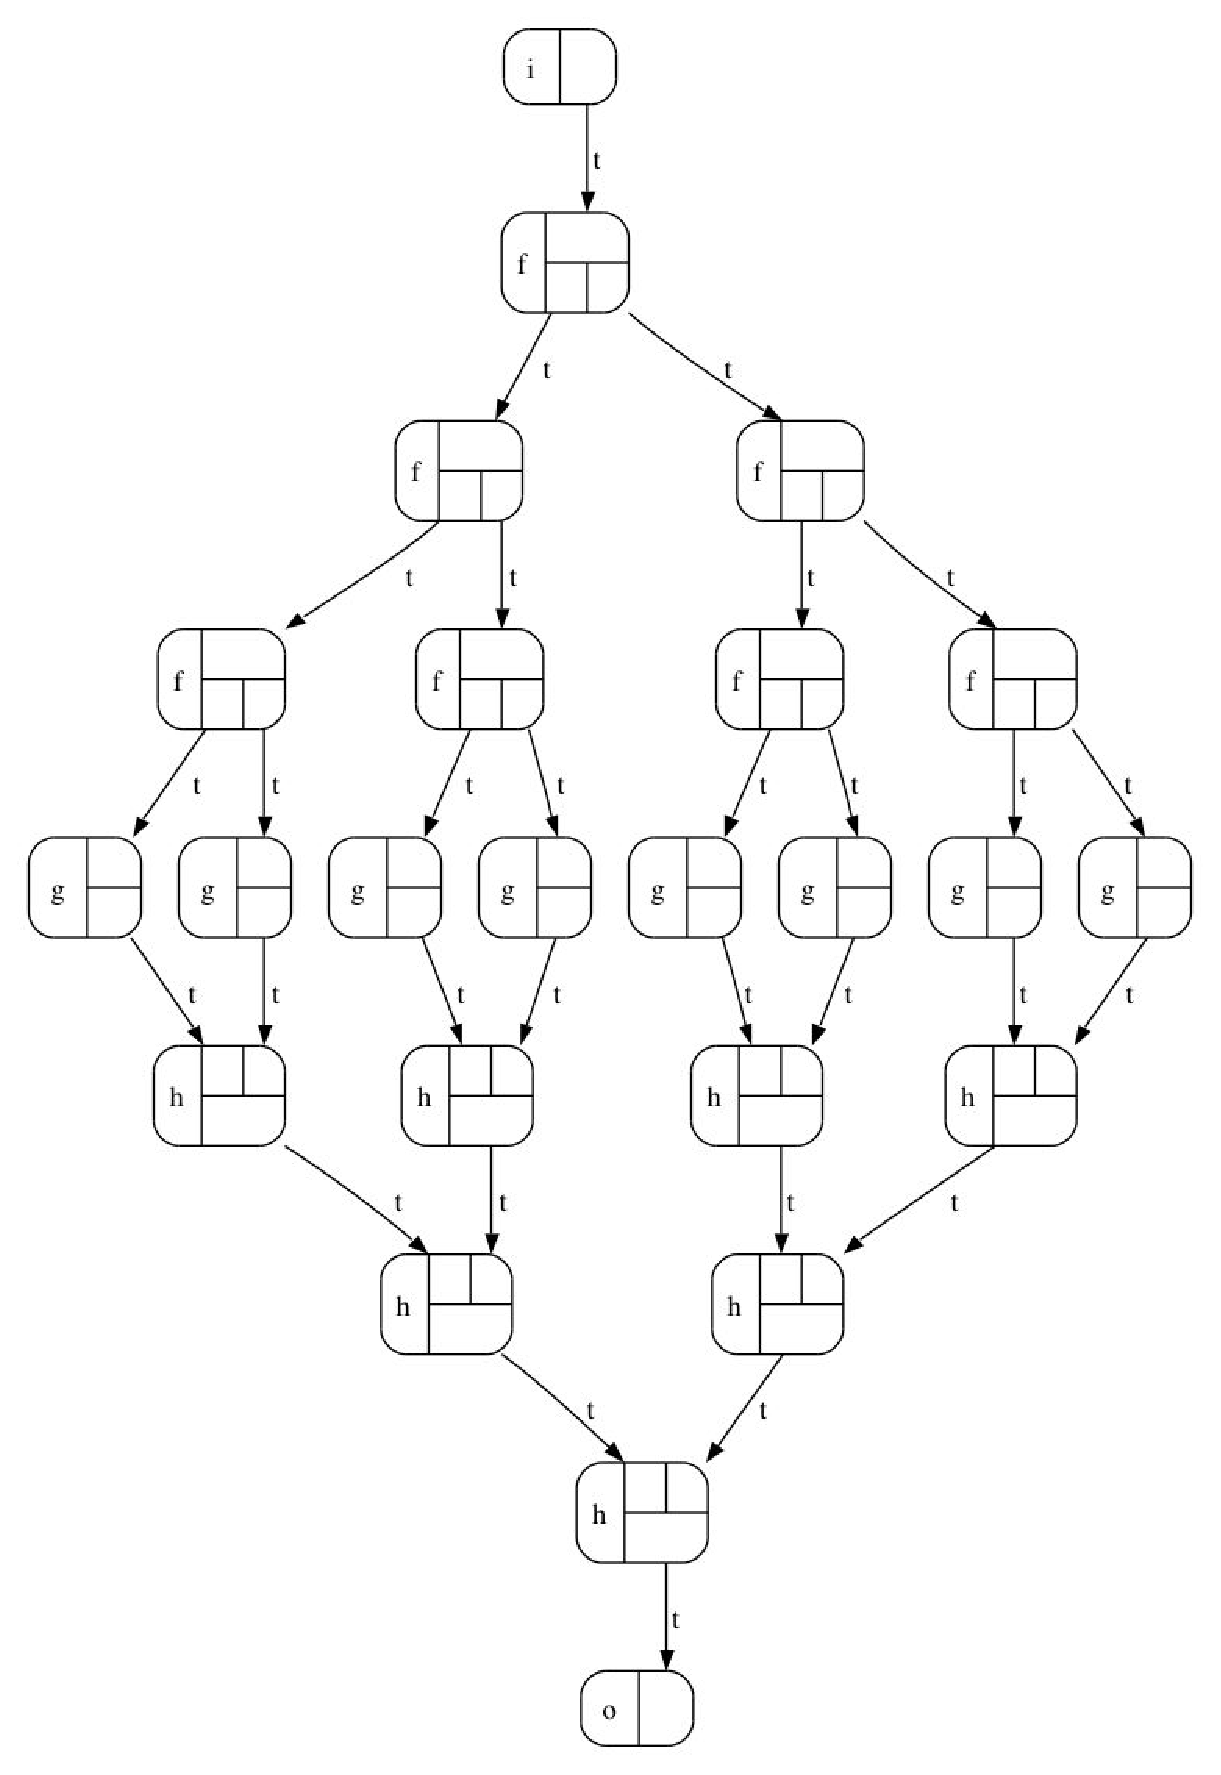
\includegraphics[width=0.85\textwidth]{figs/diamonds}
\caption{A hierachical network}
\label{fig:diamonds}
\end{center}
\end{figure}

\subsection{The actor Language}
\label{sec:actor-lang}

The \caph\ {\it actor language} is used to describe the behavior of individual dataflow actors. 
This is done using a set of \emph{transition rules}, fired according to a generalized
pattern-matching mechanism. The actions performed by each rule are described using a purely functional, primitive recursive
language with a strict semantics.

A complete description of the actor language will be given in the next chapter. In this section, we
will just introduce it using a simple example. Let us consider the actor \texttt{merge} described in
Fig.~\ref{fig:mergeactor}. This actor takes two streams of tokens as inputs and produces one stream
of tokens, taking input alternately from the first and second output.  Its behavior description in
\caph is given on the left. It has two inputs and one output, all of type \texttt{int}. It also
uses a local variable, \texttt{s}, of type \texttt{bool}.
Its behavior is specified using a set of rules defined under the \texttt{rules} keyword.
Each rule consists of a set of \emph{patterns} refering to inputs or local variables and a
corresponding set of \emph{expressions}, refering to outputs or local variables.
The first (resp. second) rule
says : If \texttt{s} is \texttt{'false'} (resp. \texttt{'true'}) and a value \texttt{v} is available
on input \texttt{i1} (resp. \texttt{i2}) then read\footnote{Pop the connected channel.}
this value, write it to output \texttt{o} and set \texttt{s} to \texttt{'true'}
(resp. \texttt{'false'}).

Fig.~\ref{fig:fouractorsdesc} gives the description in \caph of the four actors introduced in
Fig.~\ref{fig:fouractors}. 

\begin{figure}[h]
  \centering
  \includegraphics[width=\linewidth]{figs/mergeactor}
  \caption{An example of actor description in \caph}
  \label{fig:mergeactor}
\end{figure}

\begin{figure}[h]
  \centering
  \begin{tabular}[c]{cc}
    \begin{minipage}[c]{0.45\linewidth}
      \begin{lstlisting}
        actor inc 
          in (i: int)
         out (o: int)
        rules
          i:x -> o:x+1;
      \end{lstlisting}
    \end{minipage} &
    \begin{minipage}[c]{0.45\linewidth}
      \begin{lstlisting}
        actor dec 
          in (i: int)
         out (o: int)
        rules
          i:x -> o:x-1;
      \end{lstlisting}
    \end{minipage} \\
    \begin{minipage}[c]{0.45\linewidth}
      \begin{lstlisting}
        actor mul 
          in (i1: int, i2:int)
         out (o: int)
        rules
          (i1:x, i2:y) -> o:x+y;
      \end{lstlisting}
    \end{minipage} &
    \begin{minipage}[c]{0.45\linewidth}
      \begin{lstlisting}
        actor dup 
          in (i: int)
         out (o1: int, o2: int)
        rules
          i:x -> (o1:x, o2:x);
      \end{lstlisting}
    \end{minipage}
  \end{tabular}
  \caption{\caph description of the four actors introduced in Fig.~\label{fig:fouractorsdesc}}
\end{figure}



\section{Tools and design flow}

The current tool chain supporting the \caph language is sket\-ched on Fig.~\ref{fig:toolset}. It
comprises a graph visualizer, a reference interpreter and compiler producing both SystemC
and synthetizable VHDL code.

\begin{figure}[t]
  \centering
  \includegraphics[width=0.5\textwidth]{figs/toolset}
  \caption{}
  \label{fig:toolset}
\end{figure}

The \textbf{graph visualizer} produces representations of the actor network in the \texttt{.dot}
format~\cite{North1994}
for visualisation with the \textsc{graphviz} suite of tools~\cite{graphivz}.

The \textbf{reference interpreter} implements the dynamic semantics defined in
Sec.~\ref{chap:dynamic-semantics}. 
 Its role is to provide
reference results to check the correctness of the generated SystemC and VHDL code. It can also be
used to test and debug programs, during the first steps of application development (in this case,
input/output streams are read from/written to files). Several 
tracing and monitoring facilities are provided. For example, it is possible to compute statistics on
channel occupation or on rule activation.

The \textbf{compiler} is the core of the system. It relies on an \emph{elaboration phase}, turning
the AST into a target-independant intermediate representation (described in
chapter~\ref{chap:interm-repr}), and a set of dedicated back-ends.

Two back-ends are currently provided : the first produces cycle-accurate SystemC code for simulation
and profiling, the second VHDL code for hardware synthesis. Execution of the SystemC code provides
informations which are used to refine the VHDL implementation (for example : the actual size of the
FIFOs used to implement channels).

\medskip
The graph visualizer, the reference interpreter and the compiler all operate on an abstract syntax
tree (AST) produced by the \textbf{front-end} after parsing and type-checking.

%%% Local Variables: 
%%% mode: latex
%%% TeX-master: "caph"
%%% End: 

%%%%%%%%%%%%%%%%%%%%%%%%%%%%%%%%%%%%%%%%%%%%%%%%%%%%%%%%%%%%%%%%%%%%%%%%%%%%%%%%%%%%%%%%%
%%                                                                                     %%
%%                This file is part of the CAPH Compiler distribution                  %%
%%                            http:%/caph.univ-bpclermont.fr                           %%
%%                                                                                     %%
%%                                  Jocelyn SEROT                                      %%
%%                         Jocelyn.Serot@univ-bpclermont.fr                            %%
%%                                                                                     %%
%%         Copyright 2011-2018 Jocelyn SEROT.  All rights reserved.                    %%
%%  This file is distributed under the terms of the GNU Library General Public License %%
%%      with the special exception on linking described in file ..%LICENSE.            %%
%%                                                                                     %%
%%%%%%%%%%%%%%%%%%%%%%%%%%%%%%%%%%%%%%%%%%%%%%%%%%%%%%%%%%%%%%%%%%%%%%%%%%%%%%%%%%%%%%%%%

\chapter{CAPH Overview}
\label{chap:overview}

This chapter introduces the \caph language. The basic structure of programs is presented. Its syntax
and semantics are introduced informally, by means of examples. Formal accounts can be found in
chapters~\ref{chap:syntax}, \ref{chap:abssyn}, \ref{chap:typing}, \ref{chap:static} and
\ref{chap:dynamic-semantics}.  In the examples, comments follow the \caph syntax : they are
single-line and starts with ``\texttt{--}''.

\section{Language structure}
\label{sec:language-struct}

As stated in introduction, \caph is a layered language. 

The outermost (\emph{declaration}) layer declares types, global values (constant and functions), I/O streams, actors and
network-level objects (wires and wiring functions).
The innermost (\emph{expression}) layer is used for describing computations. 
An \emph{actor} sub-language is used for describing the interface and the behavior of actors and a
\emph{network} sub-language is used for describing the structure of the dataflow process network. 

All layers essentially share a common type system, which is presented in the next section.

\section{Types}
\label{sect:types}

Broadly speaking, two categories of types can be distinguished: \emph{scalar} types and
\emph{structured} types\footnote{The concept of \emph{type variable} is discussed separately in
  Sec.~\ref{sec:polymorphism}}.

\subsection{Scalar types}
\label{sec:scalar-types}

Scalar types are described in Table~\ref{tab:scalar-types}. They include signed and unsigned
fixed-precision integers, booleans and floating-point values\footnote{Support of floating-point
  values by the VHDL backend is platform-dependant (see Sec.~\ref{sec:transl-syst-vhdl}).}.

\begin{table}
\small
\begin{center}
\begin{tabular}{|l|l|} \hline
\texttt{int} & Generic (signed) integer, range is implementation dependant\\ \hline   
\texttt{signed<prec>} & Sized signed integer, range is $-2^{prec-1}\ldots 2^{prec-1}-1$\\ \hline   
\texttt{unsigned<prec>} & Sized unsigned integer, range is $0 \ldots 2^{prec}-1$\\ \hline   
\texttt{bool}       & Boolean (\verb|true|, \verb|false|) \\ \hline   
\texttt{float}       & Floating-point value (minimal range : $-1.10^{38}\ldots+1.10^{38}$)  \\ \hline   
\end{tabular}
\caption{\caph scalar types}
\label{tab:scalar-types}
\end{center}
\end{table}

\medskip
Builtin operations provided on scalar types are summarized in Table~\ref{tab:scalar-ops}.
By \emph{builtin}, we mean the operations which
\begin{itemize}
\item have a runtime implementation at the simulator level,
\item can be a automatically translated to their SystemC and VHDL equivalent by the compiler
  back-ends\footnote{The support of floating-point values ultimately depends on the VHDL compiler.}.
\end{itemize}

\begin{table}
\begin{minipage}[c]{1.0\linewidth}
\small
\begin{center}
\begin{tabular}{|l|l|} \hline
{\tt bool}      & {\tt \&\& || not} (logical and, or, not) \\ \hline 
{\tt int}       & {\tt + - * / mod} \\ 
{\tt signed}    & \tt {< <= = >= >} \\
{\tt unsigned}  & \\ \hline
{\tt signed}    & {\tt land lor lnand lnot} (bitwise operations) \\
{\tt unsigned}  & {\tt <<}, {\tt >>} (left/right logical shift)\\  \hline
{\tt float}     & {\tt +. -. *. /.}  \\
                & {\tt =. !=. <. >. <=. >=.}  \\ \hline
%                & {\tt sll srl}\footnote{These operators can also be written {\tt <<} and {\tt >>} resp.} (left/right logical shift)\\ 
%                & {\tt sla sra} (left/right arithmetic shift)\\ 
%                & {\tt rol ror} (left/right rotate) \\ \hline
\end{tabular}
\caption{Builtin operations on scalar types}
\label{tab:scalar-ops}
\end{center}
\end{minipage}
\end{table}
\normalsize

% For \texttt{word}, {\verb+ & | ^ ~+} are bitwise and, inclusive or, exclusive or
% and negation respectively.  The {\tt <<} and {\tt >>} operations pad to right/left with
% {\tt 0}s respectively, as required.

\subsection{Structured types}
\label{sec:structured-types}

Two categories of structured types are currently supported : arrays and variants.

\bigskip \textbf{Arrays} are indexed collections of values of the same type. The corresponding type,
\texttt{array}, is predefined in \caph. Arrays can have one, two or three dimensions~:
\begin{itemize}
\item for 1D arrays, each item has a scalar type,
\item 2D arrays are viewed as arrays of 1D arrays\footnote{And for this reason, sometimes called
    1D$\times$1D arrays.},
\item 3D arrays are viewed as arrays of 2D arrays\footnote{And for this reason, sometimes called
    1D$\times$1D$\times$1D arrays.}.
\end{itemize}
For each dimension, the size $S$ is fixed and must defined at the declaration. Indexes range from
$0$ to $S-1$.

Arrays can be declared either as global constants or as local variables in actors
(Table~\ref{tab:array-decls}). In the first case, the (immutable) value of the array is part of the
declaration and an optional type signature can be used to refine the type of the array items. In the
second case, the type signature is not optional but the initial value can be omitted\footnote{It is
  the progammer's responsability, of course, to ensure that no element of the array will be accessed
  before having been properly initialized.}.  Two syntaxes -- extension and comprehension -- are
provided for specifying initilisation values. 

\begin{table}
\begin{minipage}[c]{1.0\linewidth}
\small
\begin{center}
\begin{tabular}{|l|r|} \hline
\texttt{const <id> "=" <array\_init> [ ":" <array\_type> ]} & global constant \\ 
\texttt{var <id> ":" <array\_type> [ "=" <array\_init> ]} & local variable \\ 
\emph{where} & \\
\texttt{<array\_init> ::=} & \\
\hspace{0.5cm}\texttt{<array\_ext1>} & 1D extension \\
\hspace{0.5cm}\texttt{<array\_ext2>} & 2D extension \\
\hspace{0.5cm}\texttt{<array\_ext3>} & 3D extension \\
\hspace{0.5cm}\texttt{| "[" <expr> "|" <index_range> "," ..., "," <index_range>} & comprehension \\ 
\texttt{<array_ext1> ::=} & \\
\hspace{0.5cm}\texttt{| "[" <scalar\_const>\_1 "," ... "," <scalar\_const>\_n "]"} & \\ 
\texttt{<array_ext2> ::=} & \\
\hspace{0.5cm}\texttt{| "[" <array\_ext1>\_1 "," ... "," <array\_ext1>\_n "]"} & \\ 
\texttt{<array_ext3> ::=} & \\
\hspace{0.5cm}\texttt{| "[" <array\_ext2>\_1 "," ... "," <array\_ext2>\_n "]"} & \\ 
\texttt{<index\_range> ::=} & \\
\hspace{0.5cm}\texttt{| <id> "=" <index\_1> "to" <index\_2>} & \\ 
\emph{and} & \\
\texttt{<array\_type> ::=} & \\
\hspace{0.5cm}\texttt{<scalar\_type> "array" "[" <size> "]"} & 1D array \\
\hspace{0.5cm}\texttt{<scalar\_type> "array" "[" <size> "]" "[" <size> "]"} & 2D array \\
\hspace{0.5cm}\texttt{<scalar\_type> "array" "[" <size> "]" "[" <size> "]" "[" <size> "]"} & 3D array \\
\emph{Examples} & \\
\texttt{var a : signed<4> array[4]} & \\
\texttt{var b : unsigned<8> array[4] = [1,2,3,4]} & \\
\texttt{var c : unsigned<8> array[4] = [i*2 | i=0 to 3]}\footnote{This is equivalent to \texttt{var
    c : unsigned<8> array[4] = [0,2,4,6]}} & \\ 
\texttt{const a1 = [1,2,3,4] : signed<4> array[4]} & \\
\texttt{const a2 = [[1,2],[3,4],[5,6]] : signed<4> array[3][2]} & \\
\texttt{const a3 = [[[1,2],[3,4]],[[5,6],[7,8]]] : signed<4> array[2][2][2]} & \\ \hline
\end{tabular}
\caption{Array declarations}
\label{tab:array-decls}
\end{center}
\end{minipage}
\end{table}

Individual array items can be accessed for reading and updating using the classical \verb|[.]| notation
(Table~\ref{tab:array-exprs}). 

\begin{table}
\begin{minipage}[c]{1.0\linewidth}
\small
\begin{center}
\begin{tabular}{|l|r|} \hline
\texttt{<array\_id>"["<index\_expr>"]"} & for 1D arrays \\ 
\texttt{<array\_id>"["<index\_expr>"]" "["<index\_expr>"]"} & for 2D arrays \\ 
\texttt{<array\_id>"["<index\_expr>"]" "["<index\_expr>"]" "["<index\_expr>"]"} & for 3D arrays \\ 
\emph{where} & \\
\texttt{<index\_expr>} is any expression of type \texttt{int} & \\
\emph{Examples} & \\
\texttt{t[1]} & \\
\texttt{t[2*i+1]} & \\
\texttt{t[i][j]} & \\
\texttt{t[i][j][2]} & \\ \hline
\end{tabular}
\caption{Array expressions}
\label{tab:array-exprs}
\end{center}
\end{minipage}
\end{table}


% \begin{table}
% \begin{minipage}[c]{1.0\linewidth}
% \small
% \begin{center}
% \begin{tabular}{|l|l|l|} \hline
% Array declaration & \texttt{<scalar\_type> <array\_id>"["<size>[","<size'>]"]" [ "=" <array\_init> ]} \\ 
%                   & ex: \texttt{signed<4> a[4]} \\
%                   & ex: \texttt{signed<4> b[4] = [1,2,3,4]} \\
%                   & ex: \texttt{unsigned<8> c[4] = [i in 0..3 <- i*2]}\footnote{This is equivalent to \texttt{unsigned<8> c[4] = [0,2,4,6]}} \\ 
%                   & ex: \texttt{unsigned<8> c[256] = [0:256]}\footnote{This is equivalent to
%                     \texttt{unsigned<8> c[256] = [i in 0..255 <- 0]}} \\ 
%                   & ex: \texttt{signed<8> d[2,2] = [[1,2],[3,4]]} \\
%                   & ex: \texttt{signed<8> d[2,2] = [i in 0..1, j in 0..1 <- if i=j then 1 else
%                     0]}\footnote{This is equivalent to \texttt{signed<8> d[2,2] = [[1,0],[0,1]]}} \\ \hline
% Array access & \texttt{<array\_id>"["<index\_expr>"[","<index\_expr>]"]"} \\ 
%             & ex: \texttt{v := a[2]} (1D case) \\
%             & ex: \texttt{v := d[0,1]} (2D case) \\ \hline
% Array ``update'' & \texttt{<array\_id>"["<index\_expr1>"<-"<expr1>","...","<index\_exprN>"<-"<exprN>"]"} \\ 
%                  & \texttt{<array\_id>"["<id1> "in" <range1>","...","<idN> "in" <rangeN> "<-" <expr>"]"} \\ 
%              & ex: \texttt{a := b[1<-8]}\footnote{$a_i=b_i\ \forall i\not= 1, a_1=8$} \\ 
%              & ex: \texttt{b := b[1<-8,2<-6]}\footnote{$b_0=1,b_1=8,b_2=6,b_3=4$} \\ \hline
%              & ex: \texttt{b := b[i in 1 .. 2 <- b[i]*2]}\footnote{$b_0=1,b_1=16,b_2=12,b_3=4$} \\ \hline
% \end{tabular}
% \caption{Operations on arrays}
% \label{tab:array_ops}
% \end{center}
% \end{minipage}
% \end{table}

% \medskip \textbf{Vectors} are used to define higher-order wiring functions at the
% coordination level. They are only available at the coordination level.
% \tbw

\bigskip \textbf{Variants} allow values of different
kinds to be mixed together in a common type by tagging them with a distinct label. They are
described in Sec.~\ref{sec:type-declarations}.

\subsection{Translation to SystemC and VHDL types}
\label{sec:transl-syst-vhdl}

Table~\ref{tab:type-transl} describes how \caph types are translated to SystemC or VHDL types by the
compiler back-ends.

In VHDL, Tokens circulating between actors are represented as
\texttt{std\_logic\_vector}s and numeric values are represented using the
\texttt{signed} or \texttt{unsigned} data types defined in the \texttt{ieee.numeric\_std}
library\footnote{There's a compiler option to change the default library used for implementing
  arithmetic operations.}. Booleans are encoded as VHDL \texttt{boolean}s. Floating-point values are
currently encoded using the \texttt{float32} type provided by the \emph{VHDL-2008 Support Library} available
at \texttt{http://www.vhdl.org/fphdl}\footnote{This should be viewed as a temporary solution, before
  the full VHDL-2008 standard is supported by mainstream VHDL compilers and synthetizers. Support
  for floating-point values can be disabled if this library cannot be installed on the target
  platform.}.

\begin{table}
\begin{minipage}[c]{1.0\linewidth}
\small
\begin{center}
\begin{tabular}{|l|l|l|} \hline
\caph                  &  SystemC                &  VHDL \\ \hline
\texttt{bool}          & \texttt{bool}           & \texttt{boolean} \\ \hline
\texttt{int}           & \texttt{int}            & \texttt{signed<prec-1 downto 0>} \\ \hline
\texttt{signed<prec>}& \texttt{sc\_int<prec>} or \texttt{int}\footnote{Depending on whether
  \texttt{prec} resolves to a static constant or not.}   & \texttt{signed<prec-1 downto 0>} \\ \hline
\texttt{unsigned<prec>}& \texttt{sc\_uint<prec>} or \texttt{unsigned int}\footnote{Depending on whether
  \texttt{prec} resolves to a static constant or not.}   & \texttt{unsigned<prec-1 downto 0>} \\ \hline
\texttt{float}         & \texttt{float}\footnote{C native \texttt{float} type (32 bits)}   & \texttt{float32}\\ \hline
\texttt{t array[sz]}\footnote{Where \texttt{t} is a scalar type.}  & \texttt{std::array<t',sz>}  & \texttt{array (0 to sz-1) of t'} \\
                         &                           & \hspace{1cm}where \texttt{t'} is translation of type \texttt{t} \\ \hline
\texttt{t array[sz][sz']}\footnote{Where \texttt{t} is a scalar type.}  &
\texttt{std::array<std::array<t',sz>,sz'>}  &
\texttt{array (0 to sz-1) of array (0 to sz'-1) of t'} \\
                         &                           & \hspace{1cm}where \texttt{t'} is translation of type \texttt{t} \\ \hline
%\texttt{t array<sz1,sz2>}\footnote{Where \texttt{t} is a scalar type.}  & C array   & \texttt{array
%  (0 to sz1-1, 0 to sz2-2)  of t'} \\
%                        &                            & \hspace{1cm}where \texttt{t'} is translation of type \texttt{t} \\ \hline
\texttt{t}\footnote{Where \texttt{t} is a variant type.}  & \texttt{class} \ldots\footnote{See
  chapter~\ref{cha:variants-impl}.} & \texttt{std\_logic\_vector<m+n>} \\
              &         & where  \\
              &         & $m=\lceil log_2 N_c \rceil$ \\
              &         & $n=max_{i=1\ldots N_c}|\tau_i|$ \\
              &         & $N_c$ is the number of distinct tags \\
              &         & $\tau_i$ is the type of argument for tag $i$ \\
              &         & $|\tau|$ is size (in bits) of the VHDL representation for type $\tau$ \\
              &         & The $m$ MSBs are used to encode the tag. \\
              &         & The $n$ LSBs are used to encode the argument\footnote{See
                chapter~\ref{cha:variants-impl}.} \\ \hline
%\texttt{t vector}\footnote{Where \texttt{t} is \texttt{int} or \texttt{bool}.}  &
%N/A\footnote{Vectors are only used to define wiring functions. They are never manipulated
%  by actors.}  & N/A \\ \hline
\end{tabular}
\caption{Translation of types in SystemC and VHDL}
\label{tab:type-transl}
\end{center}
\end{minipage}
\end{table}

\section{CAPH expression language}
\label{sec:caph-expr-lang}

The expression language is a small, purely functional, first-order, polymorphic language with a strict
semantics. This language is used both for defining the values assigned to global constants and
functions at the declaration level and the values computed when a rule is fired at the actor level.
Its syntax broadly follows that of Caml~\cite{Caml}.

The expression language cannot manipulate functions as values, like in classical, higher-order
functional languages. This makes sense since this concept cannot be translated, in general, into
hardware.

\subsection{Constants}
\label{sec:e-constants}

Constants at the expression-level are simple constant values covering the basic \caph types
(integers and booleans). By default, integer constants are un-signed and un-sized. Signness and size
can be provided using the type coercion operator "\verb|:|" (see Sec~\ref{sec:e-coerce}). Signness
can also specified using the \verb|U| and \verb|S| suffixes or implicitely for negative ints.

\begin{lstlisting}[title=Example]
23                 -- generic int
23S                -- signed int
23U                -- unsigned int
-12                -- signed int
(12:unsigned<4>)   -- sized, unsigned int
(12:signed<8>)     -- sized, signed int
true               -- boolean
0xFA               -- hex constant
0b1001             -- binary constant
1.23               -- float constant
-2.3               -- float constant
\end{lstlisting}

Type coercion can be used to define constants with a more precise type (see Sec~\ref{sec:e-coerce}).

\subsection{Variables}
\label{sec:e-variables}

Variables appearing at the expression level are simple identifiers. These identifiers must have
been bound at the declaration layer or with an upper \texttt{let} declaration within the same
expression. Identifiers must start with a lowercase letter (symbols starting with
an uppercase letter are used to designate data constructors).

\subsection{Function application}
\label{sec:e-fun-app}

Functions are always fully applied at the expression level\footnote{This is to be contrasted to functions
  defined at the network level, where higher-order functions and partial application are supported.}. The applied
function must have been declared in the declaration layer or be a builtin primitive. Application
of builtin primitives uses the classical infix notation.

%\noindent \textbf{Example}\xrfill{.5pt}
\begin{lstlisting}[title=Example]
g (3)          -- g is function with arity 1
f (1,2)        -- f is function with arity 2
1+2            -- + is a builtin primitive
\end{lstlisting}
%\noindent \xrfill{.5pt}

\subsection{Conditionals}
\label{sec:conditionnals}

Conditional expressions always have two alternatives, depending on
the value of the discriminating expression is ({\tt true} or {\tt false}).

\begin{lstlisting}[title=Example]
if x>1 then x-1 else x
\end{lstlisting}

\subsection{Local Declarations}
\label{sec:let-decls}

Local declarations are used to bind variable(s) to expression(s) within the (limited) scope of a given
expression. The names introduced by the bindings are only visible within the target
expression. Bindings are evaluated before the target expression is evaluated.

\begin{lstlisting}[title=Example]
let x=1+2 in x*x              -- expression value is 9
let x=1+2 and y=3*4 in x+y    -- expression value is 15
\end{lstlisting}

Local declarations can be nested. This offers a way for ``breaking'' complex computations and/or
sharing intermediary results. 

\begin{lstlisting}[title=Example]
let y=2*x+1 in let z=y*y-5 in z/4
\end{lstlisting}

\noindent
The previous example is equivalent to writing \texttt{((2*x+1)*(2*x+1)-5)/4}.

\subsection{Type coercion}
\label{sec:e-coerce}

The expression language has a builtin operator (\texttt{:}) for performing type coercion.
Type coercion is often necessary to assign values a more ``precise'' type than that infered by the
type checker in order to provide the compiler back-ends enough information. 


\begin{lstlisting}[title=Example]
(1+2 : unsigned<8>)
\end{lstlisting}

Here the type inferred by the type-checker for the mere expression \texttt{1+2} is simply
the \emph{generic} type \texttt{int}\footnote{In fact, this is
  \texttt{int<s,n>} where \texttt{s} and \texttt{n} are respectively a \emph{sign variable} and a
  \emph{size} variable. The notion of type variable is discussed in Sec.~\ref{sec:polymorphism}.}. This type is
here explicitely refined to \texttt{unsigned<8>}\footnote{Where \texttt{unsigned<8>} is actually an
  abbreviation for \texttt{int<_unsigned,8>}.}.

The coercibility relation between base types is described in Table~\ref{tab:type-casting}. A \emph{S} at
intersection of row \texttt{t} and column \texttt{t'} means that type \texttt{t} can be safely
coerced to type \texttt{t'} (with no loss of information); a \emph{U} (unsafe) indicates that some information
may be lost and a \emph{F} indicates a forbidden operation.

This relation naturally extends to structured types with the same constructor and the same number of
elements. For example, type \texttt{t array[m]} can be coerced to \texttt{t' array[n]} iff
\texttt{m=n} and \texttt{t} can be coerced to \texttt{t'}.

Coercion between integer types is only accepted in two situations:
\begin{enumerate}
\item  it corresponds to a ``refinement'' of the LHS type. Examples :
  \begin{itemize}
  \item \verb|(int<8>:unsigned<8>)| is ok,
  \item \verb|(int:unsigned<8>)| is ok,
  \item \verb|(signed<n>:signed<16>)| (where \verb|n| is an unbound size variable) is ok,
  \item \verb|(unsigned<8>:int)| is forbidden,
  \item \verb|(signed<8>:signed<n>)| (where \verb|n| is an unbound size variable) is forbidden\footnote{The known size 8 cannot be ``erased''.}.
  \end{itemize}
\item it corresponds to a modification of an already known signness or size. Examples
  \begin{itemize}
  \item \verb|(signed<8>:signed<16>)| is ok 
  \item \verb|(signed<8>:unsigned<8>)| is ok (but the sign is lost),
  \item \verb|(unsigned<16>:unsigned<8>)| is ok (but the result may be truncated).
  \end{itemize}
\end{enumerate}
The compiler accepts coercions of the first kind silently and emits a warning for the second kind 
when the signness/sizes of the LHS and RHS is/are different.

\begin{table}
\begin{minipage}[c]{1.0\linewidth}
\small
\begin{center}
\begin{tabular}{|c|c|c|c|c|c|} \hline
                     & \texttt{bool}     & \texttt{int}      & \texttt{signed<n>}   & \texttt{unsigned<n>}  & \texttt{float}    \\ \hline
\texttt{bool}        & S                 & S\footnotemark[1] & S\footnotemark[1]    & S\footnotemark[1]     & S\footnotemark[1] \\ \hline
\texttt{int}         & U\footnotemark[2] & S                 & S                    & S                     & S \\ \hline
\texttt{signed<m>}   & U\footnotemark[2] & F                 & U\footnotemark[3]    & U\footnotemark[4]     & S \\ \hline
\texttt{unsigned<m>} & U\footnotemark[2] & F                 & U\footnotemark[5]    & U\footnotemark[3]     & S \\ \hline
\texttt{float}       & U\footnotemark[2] & U\footnotemark[7] & U\footnotemark[7]    & U\footnotemark[7]     & S \\ \hline
\end{tabular}
\caption{Type casting between base types}
\label{tab:type-casting}
\end{center}
\footnotetext[1]{\texttt{true} is translated to 1, \texttt{false} to 0.}
\footnotetext[2]{0 is translated to \texttt{false}, all other values to \texttt{true}.}
\footnotetext[3]{Truncature may occur if $m>n$}
\footnotetext[4]{Sign is lost. Truncature may occur if $m>n$}
\footnotetext[5]{Truncature may occur if $m>n-1$}
\footnotetext[6]{Some loss of precision may occur}
\footnotetext[7]{The fractional part is discarded. Truncature may occur}
\end{minipage}
\end{table}

\subsection{Attributes}
\label{sec:attributes}

An \emph{attribute} is a property which can be attached to certain types of value.  Examples
are the size (number of elements) of an arrays or the width (in bits) of an integer value.

\medskip
Attribute values can be retrieved using the following syntax : \verb|<value_name>`<attribute_name>|.

\medskip
A typical use is of attributes is for initializing arrays :

\begin{lstlisting}[title=Example]
var z : array[8] = [ 0 | i=0 to z`size-1 ]
\end{lstlisting}

The current version of the compiler only supports one kind of the attribute, named \verb|size|. The
meaning of this attribute directly depends on the \emph{type} of the value to which it is
attached. Table~\ref{tab:size-attr} gives its interpretation for all \caph builtin
types\footnote{The value of the \texttt{size} attribute is undefined for user-defined types.}. 

\begin{table}
\begin{center}
\begin{tabular}{|l|l|} \hline
If value \texttt{v} has type\ldots  &  \verb|v`size| gives\ldots  \\ \hline
\texttt{bool}          & 1 \\ \hline
\texttt{int<prec>}     & \texttt{<prec>} \\ \hline
\texttt{signed<prec>}& \texttt{<prec>}  \\ \hline
\texttt{unsigned<prec>}& \texttt{<prec>}  \\ \hline
\texttt{float}         & 32 \\ \hline
\texttt{t array[sz]}   & \verb|sz| \\ \hline
$\tau_1 \times \ldots \times \tau_n$            & $n$ \\ \hline
\end{tabular}
\caption{Interpretation of the \texttt{size} attribute}
\label{tab:size-attr}
\end{center}
\end{table}

\section{CAPH declaration language}
\label{sect:declaration-language}

This is the outermost layer. A \caph program is just a sequence of \emph{declarations}, which are
evaluated sequentially (in other words, the declaration of an object may refer to objects declared
before but not the other way).  Declarations concerns declares types, global values (constant and
functions), I/O streams, actors and network-level objects (wires and wiring functions).

\subsection{Type declarations}
\label{sec:type-declarations}

There are two kinds of type declarations : type synonym declarations and variant declarations.

\bigskip \textbf{Type synonym declarations} are used to introduce abbreviations to existing types.
For example, the following declaration defines a type \texttt{byte} which is a synonym to the
builtin type \verb|unsigned<8>| : 

\begin{lstlisting}[title=Example]
type byte == unsigned<8>;  -- byte is now a synomym for unsigned<8>
\end{lstlisting}

\bigskip \textbf{Variant declarations} are used to define \emph{algebraic data types}. These types
-- also called \emph{tagged unions} -- allow values of different types to be mixed together by
tagging them with a distinct label.  Consider for example the situation in which a token can carry
either a signed or unsigned 8-bit value. A type for this kind of tokens could be defined with the
following type declaration :

\begin{lstlisting}[]
type us8 = 
    Signed of signed<8> 
  | Unsigned of unsigned<8> 
\end{lstlisting}

This declaration introduces the \emph{type constructor} \verb|us8|. A value of type \verb|us8| is
either a \verb|signed<8>| value or a \verb|unsigned<8>| value. The associated tag (\verb|Signed| or
\verb|Unsigned|) is used to distinguish between these two cases.

More generally speaking, the declaration of a variant type lists all possible ``shapes'' for values of
that type. Each case is identified by a specific tag, called a \emph{value constructor}, which serves both for
constructing values of the variant type and inspecting them by pattern-matching (see
Sec.~\ref{sec:actor-examples} for examples). Value constructors can take $0$ to $n$
arguments\footnote{Since version 2.6.2. In previous versions only nullary and unary value
  constructors were supported.}. To distinguish them from variable names -- which start with a
lowercase letter -- they must start with a capital letter.

\medskip
Type constructors can be polymorphic, \ie they can be parameterized over (an)other type(s), called the
\emph{argument types(s)} (see Sec.~\ref{sec:polymorphism}). For example, here's a definition of a type
for representing \emph{optional} values (\ie values that can be either present or absent) :

\begin{lstlisting}[title=Example 1]
type $t option = 
  Absent
| Present of $t
\end{lstlisting}

A value of type \mbox{$\tau$ \texttt{option}} is either \verb|Absent| or \verb|Present v|, where
\verb|v| is a value of type $\tau$ and $\tau$ can be any type.

\medskip
The following definition introduces a type for representing optionally labeled values~:

\begin{lstlisting}[title=Example 2]
type ($t1,$t2) labeled  = 
| Unlabeled of $t1
| Labeled of $t1 * $t2
\end{lstlisting} % $

A value of type \mbox{$(\tau,\lambda)$ \texttt{labeled}} is either \verb|Unlabeled v|, where
\verb|v| is a value of type $\tau$ or \verb|Labeled (v,l)| where \verb|v| is a value of type $\tau$
and \verb|l| a value of type $\lambda$. As above, $\tau$ and $\lambda$ can be any type.

\medskip
When an variant type involves sized integers, it can be parameterized over the corresponding sizes. 
The size parameters are then specified by listing them, between \verb|<| and \verb|>| after the name
of the type constructor\footnote{This ``hybrid'' approach, in which \emph{type} parameters are
  specified using a prefix notation and \emph{size} parameters using a postfix notation may appear 
  awkward to programmers familiar to purely prefix (OCaml, for example) of purely postfix-based
  (C++, for example) notations. It has been chosen because different trials have shown us that the
  other choices actually led to slightly more verbose
  formulations to avoid parsing ambiguities.}
For example, the type \verb|us8| introduced above could be generalized as follows : 
matter
\begin{lstlisting}[]
type us<n> = 
    Signed of signed<n> 
  | Unsigned of unsigned<n> 
\end{lstlisting}

The type \verb|us| can now be used to represent values having type \verb|signed<n>| or
\verb|unsigned<n>|, where \verb|n| can be any possible value. 

\medskip 
The two kinds of polymorphism (type and size) can appear in the same declaration. Here's for example
the declation of a type \verb|tau| whose values are either a signed integers with size \verb|n| or values of
type \verb|t| :

\begin{lstlisting}[]
type $t tau<n> = 
    Left of signed<n> 
  | Right of $t
\end{lstlisting}

\bigskip
The \caph standard library defines (in \verb|lib/caph/dc.cph|) the following type\footnote{This type
  was builtin in versions prior to 2.6.2.}~:

\begin{lstlisting}[frame=none]
type $t dc = 
  Data of $t
| SoS
| EoS
\end{lstlisting}

 \medskip The \textbf{dc} type (abbreviation for \emph{data/control}) can be used to encode
 \emph{structured streams}, \ie streams in which the sequence of tokens obeys to a certain structure
 (as opposed to ``raw'' streams in which the only structure is the order in which tokens
 appears). Consider for example the stream representing a (potentially infinite) sequence of $n
 \times n$ images. Representing this sequence as a simple stream of tokens, where each token carries
 a pixel value is generally not sufficient. Most often, actors operating on this stream will need to
 detect the start and end of a single image in this stream and the start and end of individual lines
 in this image.  This need to \emph{structure} the stream of tokens can be served by dividing the
 tokens, circulating on channels and manipulated by actors, into two broad categories : \emph{data}
 tokens (carrying actual values) and \emph{control} tokens (acting as structuring delimiters). For
 the aforementionned example, one could therefore introduce the following type to represent
 sequences of images :

\begin{lstlisting}[title=Example]
type $t image =
  | SoI            -- Start of image
  | EoI            -- End of image
  | SoL            -- Start of line
  | EoL            -- End of line
  | Data of $t    -- Pixel
\end{lstlisting}

Tokens with values \verb|SoI|, \verb|EoI|, \verb|SoL| and \verb|EoL| will be control tokens
indicating the start and end of images (resp. lines) and pixels will be carried by tokens having
values \verb|Data v|. With the scheme, the $4 \times 4$ image of Fig.~\ref{fig:img4} may be represented by the following
stream of tokens:

%\footnotesize
\begin{center}
\begin{spverbatim}
SoI, SoL, Data(10), Data(30), Data(55), Data(90), EoL,
     SoL, Data(33), Data(53), Data(60), Data(12), EoL,
     SoL, Data(99), Data(56), Data(23), Data(11), EoL,
     SoL, Data(11), Data(82), Data(46), Data(11), EoL,  EoI
\end{spverbatim}
\end{center}
\normalsize

But it turns out that the type introduced above is sufficient for performing this encoding
of images as structured streams. The idea is that an image can viewed as a \emph{list} of lines,
where each line can in turn be viewed as a \emph{list} of pixels. For this, the \verb|SoS|
(resp. \verb|EoS|) is interpreted as a \emph{start of list} (resp. \emph{end of list}) control
token, and the $4 \times 4$ image of Fig.~\ref{fig:img4} is now represented by the following
stream of tokens:

%\footnotesize
\begin{center}
\begin{spverbatim}
SoS, SoS, Data(10), Data(30), Data(55), Data(90), EoS,
     SoS, Data(33), Data(53), Data(60), Data(12), EoS,
     SoS, Data(99), Data(56), Data(23), Data(11), EoS,
     SoS, Data(11), Data(82), Data(46), Data(11), EoS,  EoS
\end{spverbatim}
\end{center}
\normalsize

The advantage\footnote{Which has probably not escaped to programmers familiar with the Lisp
language\ldots} is that any kind of data structure can be represented this way : images, lists, but
also trees, \emph{etc.}, without requiring dedicated types.  

Moreover,
this structured representation of data nicely fits the stream-proces\-sing programming and execution
models.
Since the structure of the data is explicitly contained in the token stream no global control
  and/or synchronization is needed; this has strong and positive consequences both at the
  programming level (it justifies \emph{a posteriori} the style of description we introduced in the
  previous subsection for actors) and the execution level (it will greatly eases the production of
  HDL code).
Moreover, it naturally supports a pipelined execution scheme; processing of a line by an actor, for
  example, can begin as soon as the first pixel is read without having to wait for the entire structure
  to be received; this feature, which effectively allows concurrent circulation of successive
  ``waves'' of tokens through the network of actors is of course crucial for on-the-fly processing
  (like in real-time image processing).

\begin{figure}[h]
  \centering
  \includegraphics[width=4cm]{figs/datarepr}
  \caption{A $4 \times 4$ image}
  \label{fig:img4}
\end{figure}

\subsection{Value declarations}
\label{sec:value-declarations}

There are two types of value declarations : constants and functions.

Identifiers bound in these declarations scope over both the actor and network sub-languages, but
an important distinction must be made.

At the actor level, they can appear everywhere in the expressions defining the behavior of actors
(in the right-hand side of actor rules -- see Sec.~\ref{sec:actor-body}).  As a matter of fact,
global functions are often used to improve the readability of actors, by allowing a separation
between purely combinational and sequential aspects.

At the network level, they can only appear as parameters when an actor is instanciated (see
Sec~\ref{sec:network-expressions}) and cannot be used to define network-level expressions.

\subsubsection{Constant declarations}
\label{sec:const-decl}

Constant declarations are like \texttt{\#define} declarations in C. They give a name to a value which
is computed statically. They are typically used to define application-specific parameters.

\begin{lstlisting}[title=Example]
const threshold = 1+2;                -- scalar constant
const kernel = [1,2,1];               -- 1D array constant 
const kernels = [[1,2,1],[1,4,1]];    -- 1Dx1D array constant 
\end{lstlisting}

\subsubsection{Function declarations}
\label{sec:funct-decl}

Function declarations introduce functions, mapping an identifier (or a set of
identifiers) to an expression. Functions with several arguments are represented as functions taking a tuple. 
An optional type signature can be specified to refine the type of the function.

\begin{lstlisting}[title=Example]
function incr x = x+1;
function scale (x,s) = x*s : signed<8> * signed<8> -> signed<16>;
\end{lstlisting}

\subsubsection{External function declarations}
\label{sec:extern-funct-decl}

External functions declarations introduce functions which are defined outside the \caph language.
Their main usage is to allow the SystemC or VHDL generated code to make use of pre-existing
functions already written in these languages. The type of the corresponding function must be
supplied. For the corresponding program to be simulated, a Caml
implementation of the function must also be provided\footnote{It could be possible to interface the
  simulator directly to the C code but this is not currently implemented. Hence the necessity to
  provide the Caml version of the function.}.

\begin{lstlisting}[title=Example]
function sqrt x =
  extern "sqrt_c","sqrt_vhd","sqrt_ml": unsigned<16> -> unsigned<16>;
\end{lstlisting}

In the above example, \texttt{sqrt\_c}, \texttt{sqrt\_vhd} and \texttt{sqrt\_ml} are the names of
the C, VHDL and Caml implementations of the \texttt{sqrt} \caph function\footnote{We have used three
different names but in practice, the same name can be used for the three implementations.}. 
These functions are supposed to be defined in a file accessible when compiling the code generated by
the back-ends. For the ML function, it must be defined in a specific file and registered using a
dedicated function. The mechanism is detailed in Chap.~\ref{cha:foreign-funct-interf}

Its the programmer's responsability to ensure that the actual types of the function arguments and result
are compatible with the types specified in the declaration. There's currently no specific type-based
translation mechanism for foreign values. As a result, only functions whose arguments and result can
be safely coerced to integers are supported.

\subsection{I/O declaration}
\label{sec:io-declarations}

These declarations specify the way by which the application will interact with the operating system
(during simulation) or the physical devices (for the generated VHDL code for example).

Two types of I/Os are supported : \texttt{stream}s and \texttt{port}s.

\medskip
Streams are used to model pure data flows, in which tokens are read (resp. written) from (resp. to)
a sequential source (resp sink) using a fifo-like protocol. 

\medskip
Ports are used to model ``asynchronous'' I/Os, in which values are read (resp. written) using a
RAM-like interface.

\medskip
Both types of declarations specify a name, a type, a direction (input or output) and a
``device''. The device is a system-specific designator identifying the entity the input
(resp. output) data will be read from (resp. written to). When using the simulator, designators will
be simple file names. The SystemC and VHDL backends may use more system and platform specific designators. 
For port inputs, the declaration also specify an initial value\footnote{For port inputs, the device can be omitted; in
this case the port behaves as a constant generator.}. 

\begin{lstlisting}[title=Example]
stream inp1 : unsigned<8> from "sample.txt";
stream outp : signed<8> to "display:0";

port inp2: unsigned<16> from "threshold.txt" init 64;
port inp3: signed<8> init -1;
port outp2: boolean to "acks.txt";
\end{lstlisting}

\subsection{Actor declarations}
\label{sec:actor-declarations}

Each actor involved in the dataflow process network must be declared. The declaration comprises an
\emph{interface} (which is the only visible part at the network level) and a \emph{body}, describing
its behavior.

\subsubsection{Actor interface}
\label{sec:actor-interface}

The interface specifies the actor input(s), output(s) and optional parameter(s). All inputs, outputs
and parameters are typed. When building the network, inputs and outputs will be connected to
channels and parameters will be given values.

\begin{lstlisting}[title=Example]
-- This actor has one input, of type int, one output, of type bool and no parameter

actor a1
  in (x: int)
 out (y: bool)
 --  ...  actor body ...
\end{lstlisting}

\begin{lstlisting}[title=Example]
 -- This actor has two inputs, both of type signed<8>, one output, of type signed<8> and one parameter, of type unsigned<4>

actor a2 (k:unsigned<4>)
  in (e1: signed<8>, e2: signed<8>)
 out (s: signed<8>)
 --  ...  actor body ...
\end{lstlisting}

\subsubsection{Actor body}
\label{sec:actor-body}

The actor body comprises a set of local variable declarations and a set of transition rules.

\medskip
The set of \textbf{local variable declarations} can be empty. Each variable is declared with a name, a type and an
optional initial value. Variables are used to retain values between successive activations of the
actor. Their scope is limited to the actor they are defined in.

\medskip
In addition to the types defined in Sec.~\ref{sect:types}, local variables can also have an
\emph{enumerated} type. Two kinds of enumerated type are accepted : explicit enumerations  and
integer ranges.

\medskip Explicit enumerations are actually variant types for which all constructors have arity 0. 

\begin{lstlisting}[title=Example]
actor ...
 ...
var state : { S0, S1, S2 }
...
\end{lstlisting}

Declaring a local variable with such a type \emph{de facto} introduces a new type but
the corresponding type constructor is anonymous 
and the scope of the introduced data constructors (\texttt{S0}, \texttt{S1}, \ldots) is limited to
  the englobing actor\footnote{This feature was introduced precisely to avoid name conflicts that
    frequently arise if one has to declare global type and data constructors for locally defined
    values such as state variables.}.

\medskip Integer ranges may be viewed as a subset of the \verb|int| type.

\begin{lstlisting}[title=Example]
actor ...
 ...
var ctr : { 1,..,8 };
...
\end{lstlisting}

A variable with such a type can be used in any expression in which an \verb|int| can be
accepted. The main distinction is that it will be recognized as a potential
\emph{state} variable when performing abstract interpretation or FSM dumping (see
Sec.~\ref{sec:dumping-box-fsm} and chapter~\ref{cha:moc}). 

\bigskip
The behavior of an actor is specified using a set of \textbf{transition rules}. 

Each rule consists of a set of \emph{patterns}, involving inputs and local variables, and a set of
\emph{expressions}, describing modifications of outputs and/or local variables.

Each rule has the form

\begin{center}
$|\quad (\text{qual}_1:\text{pat}_1, \ldots, \text{qual}_m:\text{pat}_m) \rightarrow (\text{qual'}_1:\text{exp}_1, \ldots, \text{qual'}_n:\text{exp}_n)$
\end{center}

where
\begin{itemize}
\item $qual$ designates an input, a scalar variable or an element of an array variable,
\item $pat$ is a pattern,
\item $qual'$ designates an output, a scalar variable or an element of an array variable,
\item $exp$ is an expression.
\end{itemize}

Parens can be omitted if $m=1$ (resp. $n=1$).

\medskip
A pattern can be 
\begin{itemize}
\item a litteral constant\footnote{Constants defined in value declaration section (see
    Sec.~\ref{sec:value-declarations}) are not allowed, or, more precisely, they will be interpreted
    as a variable pattern, which is generally not what is expected.} (ex: \texttt{0}, \texttt{true},
  \ldots),
\item a variable,
\item a constant constructor (\texttt{SoS}, \texttt{EoS}, or any nullary constructor introduced by an
  enumerated type or a variant type declaration),
\item \texttt{C} \emph{p}, where
  \begin{itemize}
  \item \texttt{C} is a constructor with arity 1 (\texttt{Data} or introduced by a variant type
    declaration)
  \item \emph{p} is a pattern,
  \end{itemize}
\item the ``\_'' symbol
\end{itemize}

A pattern refers to an input or a local variable, the name of which is given by the attached qualifier.

\medskip
An expression can be
\begin{itemize}
\item any expression of the expression language defined in Sec.~\ref{sec:caph-expr-lang},
\item the ``\_'' symbol
\end{itemize}

An expression refers to an output or a local variable, the name of which is given by the attached qualifier.

\medskip
Identifiers appearing within right-hand side expressions of a rule can refer to
\begin{itemize}
\item variables introduced by patterns in the corresponding left-hand side,
\item parameters of the defined actor,
\item local variables of the defined actor,
\item global variables.
\end{itemize}

\begin{lstlisting}[title=Example]
actor foo in (i:int) out (o:int)
var v : bool
rules 
| (i:x, v:true) -> o:x+1
| (i:x, v:false) -> o:x-1;
\end{lstlisting}

In this example, we have two rules. Each rule depends on the value of the input \texttt{i} and the local
variable \texttt{v} and affects the output \texttt{o}. The patterns for the first (resp. second)
rule are \texttt{x} and \texttt{true} (resp. \texttt{x} and \texttt{false}). 
These patterns will match any configuration in which a token is present on input \texttt{i} (with a
value \texttt{x}) and the local variable \texttt{v} has value \texttt{true}
(resp. \texttt{false}). The expression for the first (resp. second) rule writes the value
\texttt{x+1} (resp. \texttt{x-1}) to the output \texttt{o}.

\begin{lstlisting}[title=Example]
actor bar in (i:int) out (o:int)
var s : int = 0
rules 
| i:x -> (o:x+s, s:s+1)
\end{lstlisting}

In this second example, the pattern of the rule will match any configuration in which a token
is present on input \texttt{i}. The corresponding expressions will write the sum of the value of
this token and the value of the local variable \texttt{s} to the output \texttt{o} and increment the
local variable \texttt{s}.

\medskip
\textbf{Variant syntax for rules}. When the rule section of actor contains several rules involving
similar qualifiers for patterns and expressions, it is possible to simplify the formulation of these
rules by prefixing them by a \emph{rule format} and omitting the individual qualifiers on
patterns and expressions. A rule format has the form

\begin{center}
$(\text{qual}_1, \ldots, \text{qual}_m) \rightarrow (\text{qual'}_1, \ldots, \text{qual'}_n)$
\end{center}

where $qual$ (resp. $qual'$) designates an input (resp. output), a scalar variable or an element of
an array variable. This rule format tells to which input (resp. output, variable or array element)
the corresponding\footnote{Where correspondance is established by position.} item of all the subsequent
rules refers. As for rules themselves, the parens can be omitted when $m=1$ (resp. $n=1$).

For example, the actor \texttt{foo} introduced above can be reformulated as 

\begin{lstlisting}[title=Example]
actor foo in (i:int) out (o:int)
var v : bool
rules (i,v) -> o
| (x, true) -> x+1
| (x, false) -> x-1;
\end{lstlisting}

Both formulation -- individual qualifiers within rules or general rule format -- are strictly
equivalent\footnote{In fact, the compiler front-end translates the latter into the former.}. In this
manual, we will freely use one or the other.

\medskip
\textbf{Semantics of rules}. At each execution cycle\footnote{The precise notion of \emph{execution cycle} is defined by the
  dynamic semantics in chapter~\ref{chap:dynamic-semantics}.}, a \emph{fireable}
rule is searched. A rule is fireable if the actual values of the
inputs and local variables match the rule pattern and if the rule expression produces values that
can be written to the involved outputs. The choice of the rule to be fired is done by sequential
pattern-matching (in other words, the first rule is tried, then the second, etc. If no rule is
fireable, the actor waits for the next execution cycle).

The special pattern ``\texttt{\_}'' means "\emph{ignore}" for inputs (\emph{i.e.} don't even read
the input) and "\emph{don't care}" for local variables.

The special expression ``\texttt{\_}'' means "\emph{ignore}" (\emph{i.e.} don't write the output)
for outputs and "\emph{don't modify}" for local variables.

% \medskip
% The precise semantics of rule firing and
% actor execution is given in chapter.~\ref{chap:dynamics}. In the sequel, we will describe it
% informally using a series of small examples.

\subsubsection{Examples}
\label{sec:actor-examples}

We now give several complete examples of actors to illustrate to concepts and notations introduced
in the previous section.

\begin{lstlisting}[caption=\relax,label=lst:caph-ex1]
actor double in (i: int) out (o: int)
rules
| i:x -> o:x*2;
\end{lstlisting}

This actor defined in listing~\ref{lst:caph-ex1} ressembles the \texttt{inc} and \texttt{dec} actors introduced in
Sec~\ref{sec:network-lang}. It has one input
and one output, of type \texttt{int}, no parameter and no local variable. There's only one rule,
which says : whenever a token is available on input \texttt{i}, read it, bind the corresponding
value to \texttt{x}, evaluate expression \texttt{x*2} and write the resulting value to output
\texttt{o}. In effect, this actor will therefore doubles each value of the input stream :
\texttt{inc:1,2,3,... = 2,4,6,...}

\begin{lstlisting}[caption=\relax,label=lst:caph-ex2]
actor scale (k:int) in (i: int) out (o: int)
rules
| i:x -> o:k*x;
\end{lstlisting}

The actor defined in listing~\ref{lst:caph-ex2} is a generalization of the previous one. It
multiplies each value of the input stream by a constant factor. The factor is a parameter. Its value
will be specified when the actor will be be instanciated (at the network level).

\begin{lstlisting}[caption=\relax,label=lst:caph-ex3]
actor mux in (i1: int, i2:int, sel:bool) out (o: int)
rules (sel,i1,i2) -> o
| (true,v1,v2) -> v1
| (false,v1,v2) -> v2;
\end{lstlisting}

The actor in listing~\ref{lst:caph-ex3} is a multiplexer : it routes its first (\texttt{i1}) or
second (\texttt{i2}) input to its output (\texttt{o}) according to the value of its third input
(\texttt{sel}). For example, if \texttt{i1=1,3,5,...}, \texttt{i2=2,4,6,...},
\texttt{sel=true,true,false,...}, then \texttt{o=1,3,6,...}. Note that a token must be present on
each input for the actor to fire and that a token is consumed on each of these inputs at each
firing. Using the ``\_'' pattern, it is possible not to consume the unselected input, as described
in listing~\ref{lst:caph-ex4}. In this case, for \texttt{i1=1,3,5,...}, \texttt{i2=2,4,6,...} and
\texttt{sel=true,true,false,...}, we have \texttt{o=1,3,2,...} (the tokens accumulate on the channel
connected to \texttt{i2}).

\begin{lstlisting}[caption=A variant of the actor described in listing~\ref{lst:caph-ex3},label=lst:caph-ex4]
actor mux_bis in (i1: int, i2:int, sel:bool) out (o: int)
rules (sel,i1,i2) -> o
| (true,v1,_) -> v1
| (false,_,v2) -> v2;
\end{lstlisting}

The actor \texttt{mux} can also be described with a single rule, using a \texttt{if}
expression\footnote{But the actor \texttt{mux\_bis} cannot !}, as shown in
listing~\ref{lst:caph-ex5}.

\begin{lstlisting}[caption=Another formulation of the actor described in listing~\ref{lst:caph-ex3},label=lst:caph-ex5]
actor mux_ter in (i1: int, i2:int, sel:bool) out (o: int)
rules (sel,i1,i2) -> o
| (s,v1,v2) -> if s then v1 else v2;
\end{lstlisting}

\begin{lstlisting}[caption=\relax,label=lst:caph-ex6]
actor sum in (i: int) out (o: int)
  var sum : int = 0
rules
| i:v -> (o:sum, sum:sum+v);
\end{lstlisting}

The actor in listing~\ref{lst:caph-ex6} is a integrator : it produces the running sum of the values present on the input
stream. For example, if \texttt{i=1,2,3,4,...}, then \texttt{o=0,1,3,7,...}. For this is uses a
local variable \texttt{sum}. The single rule says : whenever a token is available on input
\texttt{i} (with value \texttt{v}), writes the current value (\texttt{v}) of \texttt{sum} to output
\texttt{o} and add \texttt{v} to \texttt{sum}. 

\begin{lstlisting}[caption=\relax,label=lst:caph-ex7]
actor switch
  in (i:int)
  out (o1:int, o2:int)
  var s : bool = false
  rules (s,i) -> (o1,o2,s)
  | (false, v) -> (v, _, true)
  | (true, v) -> (_, v, false);
\end{lstlisting}

This actor in listing~\ref{lst:caph-ex7} is the dual of the \texttt{merge} actor introduced in
Sec.~\ref{sec:actor-lang}. It reads tokens on its input channel and alternatively routes them to its
first (``left'') and second (``right'') output. Given the stream \texttt{1,2,3,4,...} it will
produce the stream \texttt{1,3,...} (resp. \texttt{2,4,...}) on its output output \texttt{o1}
(resp. \texttt{o2}). Here, the \texttt{'\_'} symbol used in the right-hand side of a rule means that
no value is produced on the corresponding output channel.

\medskip
\emph{Note} : the previous actor can be rewritten in a slightly more self-documenting manner using
an enumerated type for variable \texttt{s}, as shown in listing~\ref{lst:switch-act}.

\begin{lstlisting}[caption=\relax,label=lst:switch-act]
actor switch_bis
  in (i:int)
  out (o1:int, o2:int)
  var s : {Left,Right} = Left
  rules (s,i) -> (o1,o2,s)
  | (Left, v) -> (v, _, Right)
  | (Right, v) -> (_, v, Left);
\end{lstlisting}

\begin{lstlisting}[caption=\relax,label=lst:caph-ex9]
actor incr
  in (a:int dc)
  out (c:int dc)
  rules a -> c
  | SoS -> SoS
  | EoS -> EoS
  | Data v -> Data (v+1);
\end{lstlisting}

The actor in listing~\ref{lst:caph-ex9} increments a \emph{structured} stream of values, as
evidenced by the type of its input and output, \texttt{int dc} (see
Sec.~\ref{sec:type-declarations}). Given the structured stream

\begin{verbatim}
SoS, Data 1, Data 2, Data 3, EoS
\end{verbatim}

on its input, it will produce the structured stream

\begin{verbatim}
SoS, Data 2, Data 3, Data 4, EoS
\end{verbatim}

on its output. Here pattern-matching is used to discriminate between control and data tokens. The rules can
be read as follows : if input is a \emph{control} token (\texttt{SoS} or \texttt{EoS}) then write
the same token on output; if input is a \emph{data} token, increment the carried value and write the
resulting data token on output.

\medskip \emph{Note}. For convenience, the \texttt{SoS}, \texttt{EoS} and \texttt{Data} constructors
may be abbreviated as \texttt{'<}, \texttt{'>} and \texttt{'} respectively. The actor of
listing~\ref{lst:caph-ex9} can therefore be rewritten in a slightly more concise manner as shown
in~listing~\ref{lst:caph-ex10}

\begin{lstlisting}[caption=A rewriting of listing~\ref{lst:caph-ex9},label=lst:caph-ex10]
actor incr_bis
  in (a:int dc)
  out (c:int dc)
rules a -> c
  | '< -> '<
  | '> -> '>
  | 'v -> '(v+1);
\end{lstlisting}

\begin{lstlisting}[caption=\relax,label=lst:suml-act]
actor suml
  in (i:int dc)
  out (o:int)
var state : {S0,S1} = S0
var sum : int = 0
rules 
  | (state:S0, i:   SoS) -> (sum:0, state:S1)
  | (state:S1, i:   EoS) -> (o:sum, state:S0)
  | (state:S1, i:Data v) -> (sum:sum+v);
\end{lstlisting}

The actor in listing~\ref{lst:suml-act} operates on a structured stream composed of a sequence of
lists, each list starting with a \texttt{SoS} token and ending with a \texttt{EoS} token. For each
list, it computes the sum of the elements. For example, if
\texttt{i=<,1,2,3,>,<,4,5,>,<,6,7,8,>,...}, then \texttt{o=6,9,21,...}. For this, it uses pattern
matching on the input to detect the start and end of each list and two local variables : a local
state (\texttt{state}), indicating whether the actor is waiting for a new list or computing the sum,
and a accumulator (\texttt{sum}) for computing the sum. The three transition rules can be read as
follows :
\begin{itemize}
\item if we are in state S0 and input token is ``\verb|<|'', then initialize sum to 0 and go to state S1;
\item if we are in state S1 and input token is ``\verb|>|'', then writes the accumulated sum to output and
  go back to state S0;
\item if we are in state S1 and input token is a data, then add the corresponding value to the accumulator.
\end{itemize}
Note that the actor blocks if the input stream is ill-formed (for example, if
\texttt{i=<,1,2,<,...}).

\begin{lstlisting}[caption=\relax,label=lst:caph-ex12]
type $t option =
  Absent
| Present of $t
;

actor count
  in (a:signed<8> option)
  out (c: signed<8>)
var s: signed<8> = 0
rules 
| a:Absent -> c:s
| a:Present x -> (c:s+x, s:s+x)
;
\end{lstlisting}

Listing~\ref{lst:caph-ex12} illustrates the declaration and use of user-defined variant types.
The \verb|count| actors produces the running sum of optional values, represented with the
\verb|option| type.
When the input token is \verb|Present v| the value \verb|v| is added to the current sum \verb|s|.
When the input token is \verb|Absent| the current sum \verb|s| is unchanged.
In both cases, the current sum is output.
For example, if the token stream on input \verb|a| is

\begin{verbatim}
Present(1), Absent, Present(5), Absent, Absent, Present(9)
\end{verbatim}

then the token stream on output \verb|c| will be

\begin{verbatim}
1,    1,      6,    6,    6,     15
\end{verbatim}

\begin{lstlisting}[caption=\relax,label=lst:caph-ex13]
type us8 =
  Signed of signed<8>
| Unsigned of unsigned<8>
;

actor add
  in (a:us8, b:us8)
 out (c: us8)
rules 
| (a:Signed s1, b:Signed s2) -> c:Signed (s1+s2)
| (a:Signed s, b:Unsigned u) -> c:Signed (s+(u:signed<8>))
| (a:Unsigned u, b:Signed s) -> c:Signed ((u:signed<8>)+s)
| (a:Unsigned u1, b:Unsigned u2) -> c:Signed ((u1:signed<8>)+(u2:signed<8>))
;
\end{lstlisting}

Listing~\ref{lst:caph-ex13} shows how to define an actor performing "mixed" (signed/unsigned) arithmetic using a
variant type.  The \verb|add| actor accepts both signed and unsigned 8-bit values and produces a sum as a
signed 8-bit value, performing type coercion as needed.  For example, if the input streams on inputs
\verb|a| and \verb|b| resp. are

\begin{spverbatim}
Signed(1), Signed(2), Signed(3), Signed(-1), Signed(-2), Signed(-3), Unsigned(1), Unsigned(2), Unsigned(3)
\end{spverbatim}

\medskip
and

\begin{spverbatim}
Signed(1), Signed(-1), Unsigned(2), Signed(1), Signed(-1), Unsigned(2), Signed(1), Signed(-1), Unsigned(2)
\end{spverbatim}

\medskip
then the output stream on \verb|c| will be

\begin{spverbatim}
Signed(2), Signed(1), Signed(5), Signed 0, Signed(-3), Signed(-1), Signed(2), Signed(1), Signed(5)
\end{spverbatim}

\subsubsection{Semantics of  pattern matching}
\label{sec:more-patt-match}

The precise semantics of rule evaluation is given in chapter~\ref{chap:dynamic-semantics}. 
Basically, when a rule is selected, the expressions given in the RHS are all evaluated in an environment
containing 
\begin{itemize}
\item builtin values,
\item globally defined values,
\item actor parameters,
\item actor local variables,
\item variables bound by pattern-matching in the corresponding LHS of the rule.
\end{itemize}

Some remarks about pattern matching :

\begin{itemize}
\item a given variable can only appear once in the same LHS; for example, the following formulation
  is not allowed :
  \begin{center}
  \begin{lstlisting}[frame=none]
  actor foo in (i1:t, i2:t') out (...)
  rules
  | (i1:x, i2:x) -> ...    
  \end{lstlisting}
  \end{center}
 This makes sense because a reference to variable \texttt{x} in the RHS would be otherwise
 ambiguous.
\item pattern-matching a local variable against a variable is possible, but not required, because local
  variable are implicitely part of the evaluation environment in the RHS; for example, the two following
  formulations are semantically equivalent\footnote{Note however that the SystemC and VHDL backends will allocate an
    extra variable for the former.} :
  \begin{center}
  \begin{lstlisting}[frame=none]
  actor foo1 in (...) out (o:t)
  var s:t
  rules
  | ..., s:v, ... -> ..., o:v, ...
  \end{lstlisting}
  \end{center}
  \begin{center}
  \begin{lstlisting}[frame=none]
  actor foo2 in (...) out (o:t)
  var s:t
  rules
  | ... -> ..., o:s, ...
  \end{lstlisting}
  \end{center}
  Of course, explicit pattern matching a local variable against a constant or a structured value is
  still useful.
\item variables introduced by pattern matching in the LHS ``shadow'' actor parameters and local
  variables; for example, in the
  following example, the value written on output \texttt{o} when the first rule is selected is that
  of input \texttt{i} and not of local variable \texttt{s} :
  \begin{center}
  \begin{lstlisting}[frame=none]
  actor foo in (i:t) out (o:t)
  var s:t
  rules
  | i:s -> o:s
  | ...
  \end{lstlisting}
  \end{center}
\end{itemize}

\subsubsection{Guards}
\label{sec:guards}

A guard is a boolean expression, the value of which is added to the conditions which
are taken into account to decide whether a rule is fireable or not.
More precisely, a rule containing a guard would be marked as fireable if :
\begin{itemize}
\item the actual values of the inputs and local variables match the rule patterns and
\item the value of the guard expression is true and
\item the involved outputs are writable.
\end{itemize}

In the current version, guards can only refer to inputs or variables appearing in the patterns of
the corresponding rule or to actor parameters.

Guards do not modify the order in which rules are scanned, which is still sequential. 

\begin{lstlisting}[title=Example]
actor thr (k:signed<8>)
  in (a:signed<8>)
  out (c:unsigned<1>)
rules a -> c
| p when p > k -> 1
| p -> 0
;
\end{lstlisting}

The \texttt{thr} actor binarizes a stream of values by comparing each of them to a given theshold
(set as a parameter). For example, given the input stream \texttt{1,8,2,18}, the actor
\texttt{thr(4)} will produce the output stream \texttt{0,1,0,1}. This actor could be written
without guard with a simple conditionnal :

\begin{lstlisting}[title=Example]
actor thr_bis (k:signed<8>)
  in (a:signed<8>)
  out (c:unsigned<1>)
rules a -> c
| 'p -> if p > k then 1 else 0
;
\end{lstlisting}


\subsection{Polymorphism}
\label{sec:polymorphism}

The ability of define \emph{polymorphic} actors and functions is an important feature of the \caph
language. Coupled with the concept of \emph{higher-order wiring functions}, described in
Sec.~\ref{sec:wire-fn-decl}, it allows in particular highly generic solutions to be described and
reused in a large variety of contexts.

\medskip
Basically, a polymorphic actor (resp. function) is an actor (resp. function) for which the type of
inputs or outputs (resp. arguments and result) is left unspecified at definition. This
implies that the behavior of this actor (resp. function) does not depend on the actual value of this
type. This is called \emph{parametric polymorphism}\footnote{By opposition to \emph{ad-hoc}
  polymorphism -- a.k.a. \emph{overloading} --, where a given function, for example, may accept
  arguments with different types, performing a computation which depends on the actual type of
  the arguments.}. 

To illustrate the need for such a feature consider for example, the basic \verb|mux_s8| actor
defined below~:

\begin{lstlisting}
actor mux_s8
  in (e1: signed<8>, e2: signed<8>, c:bool)
 out (s: signed<8>)
rules
| (c:true, e1:x, e2:_) -> s:x
| (c:false, e1:_, e2:x) -> s:x
\end{lstlisting}

This actor accepts two streams of integers and a stream of booleans. When the
boolean token is \verb|true| (resp. \verb|false|), it forwards the token present on the first
(resp. second) input to the output, discarding the token present on the second (resp. first) output.
As defined above, this actor can only be used to multiplex streams of \verb|signed<8>|
quantities. If one wants to multiplex, let say, streams of \verb|unsigned<4>| quantities, another
actor must be written :

\begin{lstlisting}
actor mux_u4
  in (e1: unsigned<4>, e2: unsigned<4>, c:bool)
 out (s: unsigned<4>)
rules
| (c:true, e1:x, e2:_) -> s:x
| (c:false, e1:_, e2:x) -> s:x
\end{lstlisting}

This is clearly redundant. Having to define a new actor for each possible type for these inputs and
output is tiresome and error-prone.

In fact, the actual type of the \texttt{e1} and \texttt{e2}
inputs and \texttt{s} output does not matter, since the corresponding values are just copied from
input to output.

The solution, in this case is to define a polymorphic actor \texttt{mux} as follows :

\begin{lstlisting}
actor mux
  in (e1: $t, e2: $t, c:bool)
 out (s: $t)
rules
| (c:true, e1:x, e2:_) -> s:x
| (c:false, e1:_, e2:x) -> s:x
\end{lstlisting}
%$

Here the type \verb|$t| is a \emph{type variable}; it stands for ``\emph{any possible type t}''. The
actual value of this type variable will be decided when the actor is instanciated as a box : it
will be the actual type of the input and output wires connected to the box. Note that the fact that
\emph{same} type variable is used for both inputs and the output implies that the corresponding
wires will be required to have the same type (forbidding for example the instanciation of this actor
as a box connected to one input of type \verb|signed<8>| and \verb|unsigned<4>| for example).

\medskip Type variables may also appear in the list of parameters and local variables of an
actor. Below is a possible definition for an actor performing a one-sample delay on lists of
values\footnote{This actor is actually defined in the library \texttt{list\_ops.cph}.} :

\begin{lstlisting}
actor dl (v:$t)                     
  in (a:$t dc)
 out (c:$t dc)
var s : {S0,S1} = S0
var z : $t
rules
| (s:S0, a:'<) -> (s:S1, c:'<, z:v)
| (s:S1, a:'p) -> (s:S1, c:'z, z:p)
| (s:S1, a:'>) -> (s:S0, c:'>)
;
\end{lstlisting}

If the input stream has type, say, \verb|unsigned<4>|, and is\footnote{We use here the abbreviated
  syntax for values of type \texttt{dc}} :

\begin{verbatim}
'< '1 '2 '3 '4 '>
\end{verbatim}

then, the processing of this stream by actor \verb|d| (with its parameter \verb|v| set to 0)
will produce the following stream :

\begin{verbatim}
'< '0 '1 '2 '3  '>
\end{verbatim}

Note that this justifies \emph{a posteriori} why the definition of the \verb|dc| type is
polymorphic.


\subsubsection{Size variables}
\label{sec:size-variables}

Sometimes, a more restricted form of polymorphism is what is
needed. Consider for example an actor performing the element-wise addition of two streams of
signed integers. A possible definition of this actor could be, for example :

\begin{lstlisting}
actor add 
  in (a: signed<8>, b:signed<8>)
 out (c: signed<8>)
rules
| (a:x, b:y) -> c:x+y
\end{lstlisting}

But, again, this definition is too restrictive since a similar one should be written for
\verb|signed<4>| integers, \verb|signed<10>| integers, \emph{etc.} One could be tempted to resort to
parametric polymorphism to ``factorise out'' this redundancy, writting the \texttt{add} actor as :

\begin{lstlisting}
actor add 
  in (a: $t, b:$t)
 out (c: $t)
rules
| (a:x, b:y) -> c:x+y
\end{lstlisting}
%$

But this does not work since the builtin \verb|+| operator, used in the right-hand-side of the rule
is \emph{not} defined for any possible type $\tau$.
What is needed here is a way of abstracting over the \emph{size} of the integer arguments and
result. For this, the \verb|add| actor must be defined as follows :

\begin{lstlisting}
actor add 
  in (a: signed<s>, b:signed<s>)
 out (c: signed<s>)
rules
| (a:x, b:y) -> c:x+y
\end{lstlisting}

Here \verb|s| denotes a \emph{size variable}; it stands for ``\emph{any possible size s}''. Like
for type variables, its actual value will be set when the \verb|add| actor gets instanciated as a
box.

\subsubsection{Sign variables}
\label{sec:sign-variables}

From what precedes, one could deduce that the type of the \verb|+| builtin function is 

\begin{lstlisting}[frame=none,linewidth=\textwidth,xleftmargin=0.2\textwidth,xrightmargin=0.2\textwidth]
signed<s> * signed<s> -> signed<s>
\end{lstlisting}

Such a type would clearly be too restrictive because it forbids the application of this
operator to \texttt{unsigned} quantities. In fact, the type\footnote{Which can be displayed by
invoking the compiler with the options \texttt{-dump\_tenv} and \texttt{-phantom\_types}} of \verb|+| is

\begin{lstlisting}[frame=none,linewidth=\textwidth,xleftmargin=0.2\textwidth,xrightmargin=0.2\textwidth]
int<g,s> * int<g,s> -> int<g,s>
\end{lstlisting}

where \verb|g| is a \emph{sign variable}. A sign variable is an type variable which can only take
two values : \texttt{_signed} or \texttt{_unsigned}. In fact the types \verb|signed<n>| and
\verb|unsigned<n>| are just shorthands for \verb|int<_signed,n>| and \verb|int<_unsigned,n>|
respectively. Explicit reference to sign variables is useful when the related actor (or function)
should abstract over the signness of the manipulated integer quantities. For example, a fully
generic version of the \verb|add| actor introduced above can be written as 

\begin{lstlisting}
actor add 
  in (a: int<g,s>, b:int<g,s>)
 out (c: int<g,s>)
rules
| (a:x, b:y) -> c:x+y
\end{lstlisting}

Note that the signature of the \verb|add| actor enforces that its inputs and output have both the same
signness and size. 

This kind of signature is used largely in the CAPH standard library to define actors and wiring
functions operating both on signed and unsigned data flows (filters and convolutions for example).

\subsubsection{Note}
\label{sec:full-depdt}

The notions of size and sign variables introduced above are just an special
form of classical Hindley-Millner style of parametric polymorphism\footnote{Technically speaking,
  the type of \texttt{+} or \texttt{add} is simply the \emph{type scheme} : $\forall \alpha,\beta.~
  (\alpha,\beta)~ \mathsf{int} \times (\alpha,\beta)~\mathsf{int} \rightarrow
  (\alpha,\beta)~\mathsf{int}$.}. Size variables, in particular, cannot be used to express
dependencies richer than mere equality between sizes in type signatures. Concretely, this means that
it is not possible to define actors like 

\begin{lstlisting}[frame=none,linewidth=\textwidth,xleftmargin=0.2\textwidth,xrightmargin=0.2\textwidth]
signed<s> * signed<s> -> signed<s+1>
\end{lstlisting}

or

\begin{lstlisting}[frame=none,linewidth=\textwidth,xleftmargin=0.2\textwidth,xrightmargin=0.2\textwidth]
signed<s> * signed<s> -> signed<2*s>
\end{lstlisting}

where some kind of "computation" is allowed on type size parameters.  Supporting this would require
a significantly more complex type system than actually implemented\footnote{With full-fledged
  dependent types and constraint-solving based unification.}.

\subsubsection{Dependent types}
\label{sec:dependent-types}

\caph offers a limited form a so-called \emph{dependent typing}, in which the \emph{type} of an
actor can depend on the \emph{value} of its parameters\footnote{This feature, introduced in version
  2.6.0, is still largely experimental.}. 

\medskip
To understand why this feature is useful, consider the program given in
listing~\ref{lst:caph-deptyp-ex1}~.

\begin{lstlisting}[caption=A small program exhibiting the need for dependent types,frame=single,label=lst:caph-deptyp-ex1]
actor add
   in (i1:unsigned<s>, i2:unsigned<s>)
  out (o:unsigned<s>)
rules
| (x,y) -> x+y;

stream inp1: int<16> from "inp1.txt";
stream inp2: int<16> from "inp2.txt";
stream outp: int<16> to "res.txt";

net outp = add (inp1,inp2);
\end{lstlisting}

Now, suppose that the type network output \verb|outp| -- which is ultimately imposed by the hardware context -- is
finally changed to \verb|unsigned<12>| (with the inputs still having type \verb|unsigned<16>|).  The
actor \verb|add| cannot be used ``as is'' any longer because its signatures enforces that its inputs and output
have the same size. Of course, we could rewrite it as follows to meet the new requirements :

\begin{lstlisting}[frame=none]
actor add
   in (i1:unsigned<16>, i2:unsigned<16>)
  out (o:unsigned<12>)
rules
| (i1:x,i2:y) -> o:(x+y:unsigned<12>);
\end{lstlisting}
 
But this obviously breaks the genericity of the actor and the more general principle of modularity.
If we don't want -- or can't, because it's part of a pre-existing, otherwise used library, for
example -- to modify the \verb|add| actor, the only solution is to insert, between the output of the
\verb|add| actor and the network output \verb|outp|, an actor -- let's call it \verb|resize| -- whose function is
precisely to adjust the size of its argument. In our particular case, the signature of this actor
would be :

\begin{center}
\verb|resize : unsigned<n> -> unsigned<12>|
\end{center}

and our program could be rewritten as in listing~\ref{lst:caph-deptyp-ex2}.

\begin{lstlisting}[caption=The program of listing~\ref{lst:caph-deptyp-ex1} rewritten,frame=single,label=lst:caph-deptyp-ex2]
actor add ... -- unchanged
actor resize
  in (i:unsigned<n)
 out (o:unsigned<12>)
rules
| i:x -> o:(x:unsigned<12);

stream inp1: int<16> from "inp.txt";
stream inp2: int<16> from "inp.txt";
stream outp: int<16> to "res.txt";

net outp = resize (add (inp1,inp2));
\end{lstlisting}

But, of course, the need then quickly arises for a \emph{generic} version of the \verb|resize| actor, so that we
don't have to write a new one for each value of the output size. The idea is to make this size
a \emph{parameter} of the actor, so that, in our case, the last line of the last program 
could be written :

\begin{lstlisting}[frame=none,numbers=none]
net outp = resize 12 (add (inp1, inp2));
\end{lstlisting}

For this, the \verb|resize| actor has to be defined as follows :

\begin{lstlisting}[caption=none,frame=single]
actor resize (k:int)
  in (i:unsigned<n)
 out (o:unsigned<k>)
rules
| i:x -> o:(x:unsigned<k);
\end{lstlisting}

The type of the \verb|resize| actor is now 

\begin{center}
\verb|resize : k:int -> unsigned<n> -> unsigned<k>|
\end{center}

Such a type is called a \emph{dependent type} because the \emph{type} of some its components (the result here) depends on
the \emph{value} that will be assigned to some of the others (the first argument here). This dependency
is here explicited by naming the first argument (parameter)\footnote{Internally, the compiler uses
  on a nameless mechanism, similar to DeBruijn indices for representing dependent types. The type or
  \texttt{resize}, in particular, will be denoted  $\forall n.~\mathtt{int} \rightarrow
  \tyunsigned{n} \rightarrow \tyunsigned{@1}$, where \texttt{@1} designates the first argument.}. 

\medskip In the previous example, the value of a parameter was used to define the size of some
input/output types. This value can also be used to refine the type of some local variables of the
actor. This is specially useful for arrays when the size of the array ultimately depends on the
input data. In this case, specifying this size as a parameter value to the corresponding actor
instance may be more efficient than fixing it in the actor definition itself. As an example,
consider the \verb|dkl| actor described in listing~\ref{lst:caph-deptyp-ex3}\footnote{This actor is
  included in the standard prelude.}. This actor inserts $k$ predefined values at the beginning of a
list, discarding the same number of values of values at the end\footnote{If lists represents fixed
  size of samples or lines of an images, this operation is a ``delay'', hence the name of the
  actor.}. For this it uses a local array (\verb|z|) for memorizing the ``delayed'' values. The size
of this array obviously depends on the value of $k$ parameter. Dependent typing nicely supports this
kind of dependency\footnote{Without it, the only solution is to set the size of the array to a
  ``maximal'' value which is both dangerous (what if the actor is instanciated actor violates this
  assumption) and inefficient (leading to a waste of resources if the size of the array is
  over-estimated) in a partcular case.}. 

\begin{lstlisting}[caption=The \texttt{dkl} actor,frame=single,label=lst:caph-deptyp-ex3]
actor dkl (k:int, v:$t)
  in (a:$t dc)
  out (c:$t dc)
var s : {S0,S1,S2} = S0
var z : $t array[k] = [ v | i = 0 to k-1 ]
var i : int
rules
| (s:S0, a:'<)            -> (s:S1, c:'<, i:0)
| (s:S1, a:'p) when i<k-1 -> (s:S1, c:'v, i:i+1, z[i]:p)
| (s:S1, a:'p)            -> (s:S2, c:'v, i:0, z[i]:p)
| (s:S2, a:'p)            -> (s:S2, c:'z[i], i:if i<k-1 then i+1 else 0,
                              z[i]:p)
| (s:S2, a:'>)            -> (s:S0, c:'>)
;
\end{lstlisting}
%$

\subsection{Higher order actors}
\label{sec:higher-order-actors}

Higher order actors are an important feature\footnote{Introduced in version 2.8.} of the the CAPH
language. Just like higher order functions are functions taking other functions as argument in
classical functional programming languages, higher order (HO) actors are actors for which at least
one parameter is a function.

The possibility to define and use HO actors significantly increases the abstraction level of
programs.  Consider for example, the program given in listing~\ref{lst:caph-ho-ex1}, which defines
and then uses two actors, \verb|inc| and \verb|double|. The \verb|inc| actor takes a stream of
signed integers and produces a stream in which all data tokens have been incremented by one, whereas
the \verb|double| actor multiplies each data token by two\footnote{So that, if the input stream
  \texttt{i} is, for example, \texttt{< 1 2 3 >}, then the output streams \texttt{o1} and
  \texttt{o2} will be \texttt{< 2 3 4>} and \texttt{< 2 4 6 >} respectively.}.  Both actors exhibit
a very similar structure, only differing in the function applied to data tokens (in the third
rule). It is natural, then, to view these actors as two instances of a more general actor -- let's
call it \verb|stream_apply| -- taking a function \emph{f} as parameter and applying this function to
each data token of its input stream to produce the result stream. This actor \verb|stream_apply| is
defined in listing~\ref{lst:caph-sapp1}. The type of its parameter $f$ is
\verb|signed<m> -> signed<m>|, \emph{i.e.} the type of a function taking a value of type
\verb|signed<m>| and returning a value of the same type. This type is a hallmark of higher
order actors. Note that it is closely related to those of the actor input and output : since the
$f$ function is applied to data tokens read on an input having type \verb|signed<m> dc|, its domain
type must be \verb|signed<m>|. Respectively, since the result of this function is encapsulated in a
token having type \verb|signed<m> dc|, its co-domain type must be \verb|signed<m>|. The program of listing~\ref{lst:caph-ho-ex1} can be rewritten using the \verb|stream_apply|
actor as illustrated in listing~\ref{lst:caph-ho-ex2}.

\begin{lstlisting}[caption=A small program showing two similar actors,frame=single,label=lst:caph-ho-ex1]
actor inc
  in (i:signed<m> dc)
  out (o:signed<m> dc)
rules i -> o
| '< -> '<
| '> -> '>
| 'x -> 'x+1
;

actor double
  in (i:signed<m> dc)
  out (o:signed<m> dc)
rules i -> o
| '< -> '<
| '> -> '>
| 'x -> 'x*2
;

stream i:signed<8> dc from ...
stream o1:signed<8> dc to ...
stream o2:unsigned<16> dc ...

net o1 = inc i;
net o2 = double i;
\end{lstlisting}

\begin{lstlisting}[caption=The \texttt{stream\_apply} actor,frame=single,label=lst:caph-sapp1]
actor stream_apply (f:signed<m> -> signed<m>)
  in (i:signed<m> dc)
  out (o:signed<m> dc)
rules i -> o
| '< -> '<
| '> -> '>
| 'x -> 'f(x)
;
\end{lstlisting}

\begin{lstlisting}[caption=The program of listing~\ref{lst:caph-ho-ex1} rewritten using the actor
  defined in listing~\ref{lst:caph-sapp1},frame=single,label=lst:caph-ho-ex2]
function f_inc x = x+1 : signed<8> -> signed<8>;
function f_double x = x*2 : signed<8> -> signed<8>;

actor stream_apply (f:signed<m> -> signed<m>)
  in (i:signed<m> dc)
  out (o:signed<m> dc)
rules i -> o
| '< -> '<
| '> -> '>
| 'x -> 'f(x)
;

stream i:signed<8> dc from ...
stream o1:signed<8> dc to ...
stream o2:signed<8> dc to ...

net o1 = stream_apply f_inc i;
net o2 = stream_apply f_double i;
\end{lstlisting}

\medskip
The \verb|dc.cph| standard library (defined in \verb|lib/caph|) defines several common higher order
actors to operate on structured streams.

\medskip
The \verb|smap| actor, for instance, is a generalisation of the \verb|stream_apply| actor introduced
above, in which the applied function has the generic type $t_1 \rightarrow t_2$~:

% It can be defined formally as\footnote{Denoting "$\text{act}(p):v$" the application of actor
%   $act$, with effective parameter $p$, to value $v$.}~:
% \medskip
% \begin{math}
% \text{smap}(f):v = 
% \begin{cases}
% \mathsf{SoF} & \text{si}\ v=\mathsf{SoF}, \\
% \mathsf{EoF} & \text{si}\ v=\mathsf{EoF}, \\
% \mathsf{Data}(f(x)) & \text{si}\ v=\mathsf{Data}(x)
% \end{cases}
% \end{math}

\begin{lstlisting}
actor smap (f:$t1->$t2)
  in (i:$t1 dc)
 out (o:$t2 dc)
rules
| i:SoS    -> o:SoS
| i:Data x -> o:Data (f(x))
| i:EoS    -> o:EoS;
\end{lstlisting}

\noindent
For example, if \verb|f_inc| is a function incrementing its argument by one (just like in the first
example)\footnote{and denoting "$\text{act}_p\ (\langle\ x_1\ \ldots\ x_n\ \rangle)$" the
  application of actor $act$, with effective parameter $p$, to a streams $s=\langle\ x_1\
  \ldots\ x_n\ \rangle$.}, we have~:
\begin{equation*}
  \text{smap}_{f\_inc}\ (\langle\ 1\ 2\ 3\  \rangle) = \langle\ f\_inc(1)\ f\_inc(2)\
  f\_inc(3)\ \ \rangle = \langle\ 2\ 3\ 4\ \rangle
\end{equation*}

\medskip
The \verb|smap2| actor is a variant of \verb|smap| operating on two parallel streams~:

\begin{lstlisting}
actor smap2 (f:$t11*$t12->$t2)
  in (i1:$t11 dc, i2:$t12 dc)
 out (o:$t2 dc)
rules
| (i1:SoS, i2:SoS)       -> o:SoS
| (i1:Data x, i2:Data y) -> o:Data (f(x,y))
| (i1:EoS, i2:EoS)       -> o:EoS ;
\end{lstlisting}

For example, if \verb|add| is a function adding its two arguments, we have~:
\begin{equation*}
  \text{smap2}_{add}\ (\langle\ x_1\ \ldots\ x_n \rangle, \langle\ y_1\ \ldots\ y_n \rangle) = \langle\
  x_1+y_1\ \ldots\ x_n+y_n\ \rangle
\end{equation*}

\medskip
The \verb|sfold| higher order actor ``reduces'' structured streams by applying a reducing function
over each list of this stream. Formally :
\begin{equation*}
  \text{sfold}_{f,z}\ (\langle\ x_1\ x_2\ \ldots\ x_n \rangle) = f (f (f (f (z,x_1),x_2) ..., x_n)
\end{equation*}
For example :
\begin{equation*}
  \text{sfold}_{+,0}\ (\langle\ 1\ 2\ 3\ \rangle) = 0 + 1 + 2 + 3 = 6
\end{equation*}

\medskip
The \verb|ssfold| actor is a generalisation of the \verb|sfold| operating on lists of
lists. Formally, if we note $\l_i = \langle\ x_{i,1}\ x_{i,2}\ \ldots\ x_{i,m_i}\ \rangle$~:
\begin{equation*}
  \text{ssfold}_{f,z}\ (\langle\ l_1\ \ldots\ l_n \rangle) = \langle\ \text{sfold}_{f,z}(l_1)\
    \ldots\ \text{sfold}_{f,z}(l_n)\ \rangle
\end{equation*}
For example :
\begin{equation*}
  \text{ssfold}_{+,0}\ (\langle\ \langle\ 1\ 2\ 3\ \rangle\ \langle\ 4\ 5\ 6\ \rangle\ \rangle) =
  \langle 0+1+2+3\quad 0+4+5+6 \rangle = \langle\ 6\ 15 \rangle
\end{equation*}

\medskip
The \verb|dc.cph| library defines several variant and extensions of the HO actors : \verb|smapi|,
when the applied function also depends on the position of the data in the stream, \verb|sfold2|, for
reducing two parallel stream, \emph{etc.}

\subsection{Network declarations}
\label{sec:network-declarations}

The network language is used to define the network of actors which describes the application. 
This involves defining how actors are instanciated and the interconnection between these instances.
The basic concepts have been introduced in Sec.~\ref{sec:network-lang}. 
Two kinds of values are declared for this : \emph{wires} and \emph{wiring functions}.

\subsubsection{Wires}
\label{sec:wire-decl}

Wire declarations bind an identifier (resp. set of identifiers) to a wire (resp. set of wires) obtained
when instanciating an actor or a network of actors.

\noindent
Wire declarations have the form 

\begin{center}
\texttt{net} $<$\emph{network\_pattern}$>$ = $<$\emph{network\_expression}$>$
\end{center}


where 
\begin{itemize}
\item $<$\emph{network\_pattern}$>$ is either a single identifier or a comma-separated list of
  identifiers enclosed in brackets (a so-called \emph{tuple pattern}),
\item $<$\emph{network\_expression}$>$ is an expression representing a (sub)network of actors.
\end{itemize}

The previous declarations bind the output(s) of this network to the identifier(s) appearing in the
pattern, offering a
means to subsequently ``wire'' the corresponding output(s).

\subsubsection{Network expressions}
\label{sec:network-expressions}

Network expressions can be classified into two main categories :
\begin{itemize}
\item expressions representing sub-network of actors,
\item expressions denoting values to be used as actor parameters.
\end{itemize}

\medskip
The \textbf{first category} is described by the syntax given in Fig.~\ref{fig:ndl-syntax1} (this is an
excerpt from the full concrete syntax description given in Chap.~\ref{chap:syntax}) :

%\setlength{\grammarparsep}{20pt plus 1pt minus 1pt} % increase separation between rules
\setlength{\grammarindent}{6em} % increase separation between LHS/RHS 
\renewcommand{\litleft}{\texttt{"}}
\renewcommand{\litright}{\texttt{"}}

\begin{figure}[h!]
  \centering
  \begin{tabular}[c]{ll}
    \begin{minipage}[c]{0.75\linewidth}
\begin{grammar}
<net_expr> ::=
   <simple_net_expr>
 \alt <simple_net_expr> <simple_net_expr>+
 \alt \lit{(} <net_expr> \lit{,} ... \lit{,} <net_expr> \lit{)}
 \alt \lit{let} [ \lit{rec} ] <net_bindings> \lit{in} <net_expr>
 \alt \lit{function} <net_pattern> \lit{\texttt{->}} <net_expr>

<simple_net_expr> ::=
    <var>       
\alt \lit{(} <net_expr> \lit{)}
\end{grammar}
    \end{minipage} &
    \begin{minipage}[c]{0.25\linewidth}
-- application \\
-- t-uple \\
-- local definition \\
-- function definition \\
\\
-- identifiers
    \end{minipage}
  \end{tabular}
  \caption{Syntax of the network language (excerpt)}
  \label{fig:ndl-syntax1}
\end{figure}

\medskip
Within this category

\begin{itemize}
\item \emph{identifiers} refer either to previously defined wires, stream inputs or actors.

\item \emph{applications} ``apply'' a network expression to set of network expressions; two kind of values can be
applied :
\begin{itemize}
\item actors, like in the previous example, 
\item wiring functions, which are described in the next section.
\end{itemize}

In the former case, two kinds of arguments must be supplied, depending on whether the applied actor
has been declared with parameters or not.

\begin{itemize}

\item 
When the applied actor has no parameter, then the argument must be a single identifier, or a tuple of identifiers. For
example, if an actor \texttt{add} has been defined as 

\begin{lstlisting}
actor add 
  in (a: signed<8>, b: signed<8>)
 out (c: signed<8>)
...
\end{lstlisting}

then its application will be denoted as

\begin{lstlisting}
net x = ...
net y = ...
net r = add (x,y);
\end{lstlisting}

\item 
When the applied actor accepts parameters, then the value(s) of the parameter(s) must be passed as
an extra argument \emph{before} the wire arguments.

\emph{Example 1}. Consider an actor \texttt{scale},
accepting one parameter \texttt{k} and one input \texttt{a} defined as~:

\begin{lstlisting}
actor scale (k:signed<8>)
  in (a: signed<8>)
 out (c: signed<8>)
rules
| a:x -> c:k*x
\end{lstlisting}

then its application will be denoted, taking \texttt{k=2} here for example, as

\begin{lstlisting}
net x = ...
net r = scale 2 x;
\end{lstlisting}

\emph{Example 2}. Consider now an actor \texttt{scale2}, accepting two parameters, \texttt{k1}
\texttt{k2}, and two inputs, \texttt{a} and \texttt{b}, defined as~:

\begin{lstlisting}
actor scale2 (k1:signed<8>, k2:signed<8>)
  in (a1: signed<8>, a2:signed<8>)
 out (c: signed<8>)
rules
| (a1:x, a2:y) -> c:k1*x+k2*y
\end{lstlisting}

then its application will be denoted, taking \texttt{k1=2} and \texttt{k2=3} here, as

\begin{lstlisting}
net x = ...
net y = ...
net r = scale2 (2,3) (x,y);
\end{lstlisting}
\end{itemize}

\item \emph{Tuple patterns and expressions} are used to simultaneously bind several identifiers, like in

\begin{lstlisting}
net (x2,x3) = (scale 2 x, scale 3 x)
\end{lstlisting}

where the \texttt{scale} actor defined above is instanciated twice.

\item \emph{local definitions}, introduced with the \texttt{let \ldots in \ldots},
construct,  bind an identifier (or a set of identifiers) to an
expression with a limited scope. The name(s) introduced by the binding is (are) only visible within the target
expression. The special case of \emph{recursive} local definitions is discussed in
Sec~\ref{sec:recursive-wiring}. 

\end{itemize}

The \textbf{second category} of network expressions is used to represent values to be passed as
parameters to actors (such as \verb|2| and \verb|(2,3)|) in the examples given above, respectively).
These values are limited to~:
\begin{itemize}
\item identifiers refering to globally defined values,
\item scalar or array constants,
\item tuples of the above.
\end{itemize}

\subsubsection{Wiring functions}
\label{sec:wire-fn-decl}

As introduced in Sec.~\ref{sec:network-lang}, wiring functions simplifies the description of complex
networks by allowing the definition of reusable, polymorphic \emph{network patterns}.
Wiring function declarations have the form\footnote{Actually, and as evidenced by the abstract
  syntax of the language given in Chap.~\ref{chap:abssyn}, there's no distinction wire declarations
  and wiring function declarations. The latter is just a syntactic shorthand. In fact, there's an
  extra case to the rule defining the syntax of expressions~:
  \begin{grammar}
  <net_expr> ::= ...
    \alt \lit{function} \synt{simple_net_pattern} \lit{\texttt{->}} \synt{net_expr}
  \end{grammar}
  and the declaration \texttt{net f <pat> = <exp>} is handled as \texttt{net f = function <pat> -> <exp>}.}~:

\begin{center}
\texttt{net} \emph{fid} $<$\emph{network\_pattern}$>$ = $<$\emph{network\_expression}$>$
\end{center}

where \emph{fid} is the name of the function and \emph{network\_pattern} gives the name(s) of the
formal argument(s)\footnote{\emph{Recursive} network definitions are discussed separately in
  Sec~\ref{sec:recursive-wiring}.}.

Application of such a function follows the classical strict, \emph{call-by-value} evaluation
strategy~: each supplied argument is evaluated\footnote{Since all network expressions are pure --
  \emph{i.e.} cannot involve side-effects --, the order of evaluation is irrelevant here.} and the
resulting value is bound to the corresponding formal argument; the right-hand side expression is
then evaluated in an environment augmented with the resulting bindings.

\begin{lstlisting}[caption=\relax,label=lst:caph-ex14]
net inc2f x = inc (inc x);
net o = inc2f i;
\end{lstlisting}

In the example given listing~\ref{lst:caph-ex14}, the \texttt{inc2f} function represents a network in which
the output wire (\texttt{y}) is obtained by having the input wire (\texttt{x}) traversing two
\texttt{inc} boxes. It could be represented by the ``sub-network''of
Fig.~\ref{fig:inc2f}\footnote{The term sub-network is used here because there's no real input nor
  output, only ``slots'' -- drawn as small square boxes in Fig.~\ref{fig:inc2f} -- intended to be
  connected to actual wires }.  The application of this function at line 2 \emph{instanciates} this
sub-network and creates the network of Fig.~\ref{fig:inc2fapp}, in which the sub-network input
(resp. output) has been bound to actual the input (resp. output) \texttt{i} (resp. \texttt{o}).

\begin{figure}[h]
  \centering
  \includegraphics[height=2cm]{figs/inc2f}
  \caption{A representation of the \texttt{inc2f} wiring function defined in
    listing~\ref{lst:caph-ex14}}
  \label{fig:inc2f}
\end{figure}
 
\begin{figure}[h]
  \centering
  \includegraphics[height=1.5cm]{figs/smallnet2}
  \caption{The network resulting from applying the \texttt{inc2f} function}
  \label{fig:inc2fapp}
\end{figure}

\medskip
Wiring functions can take several arguments. In this case, arguments can be passed either as a tuple
or as a sequence.

\begin{lstlisting}[title=Example]
net foo (x,y) = add (x, inc y);
net o = foo (i1,i2);
\end{lstlisting}

The previous example could also have been written (strictly equivalent form)~: 

\begin{lstlisting}
net foo x y = add (x, inc y);
net o = foo i1 i2;
\end{lstlisting}

When this second definition form for the \texttt{foo} function\footnote{Technically known as the
  \emph{curried} form.} is used as above, it is strictly equivalent to the first one (in other
words, the network corresponding to the two previous programs are identical). But the second form
has a bonus~: it allows \emph{partial application} of the \texttt{foo} function. Partial application
means fixing the value of some arguments to obtain another function, which can be viewed as
``specialized'' version of the original one. In our case, partial application means fixing some part
of the sub-network defined by the original function.
For example, if we write

\begin{lstlisting}
net foo1 = foo i;
\end{lstlisting}

then \texttt{foo1} is the function obtained by assigning the value \texttt{i} to \texttt{x} in the
definition of \texttt{foo} (Fig.~\ref{fig:addinc}). In other words, the
\texttt{foo1} function is equivalent to the function that could have been written as

\begin{lstlisting}
net foo2 y = add (i, inc y);
\end{lstlisting}


\begin{figure}[h]
\begin{tabular}[c]{cc}
\begin{minipage}[b]{0.5\linewidth}
\begin{center}
\includegraphics[width=0.5\linewidth]{figs/addinc}
%\caption{\texttt{net foo = add (x, inc y)}}
%\label{fig:addinc1}
\end{center}
\end{minipage}
&
\begin{minipage}[b]{0.5\linewidth}
\begin{center}
\includegraphics[width=0.5\linewidth]{figs/addinc2}
%\caption{\texttt{net foo1 = foo i}}
%\label{fig:addinc2}
\end{center}
\end{minipage} \\
\texttt{net foo = add (x, inc y);} &
\texttt{net foo1 = foo i;}
\end{tabular}
\caption{Partial application}
\label{fig:addinc}
\end{figure}

Then, the three programs of Fig.~\ref{fig:threepgms} are stricly equivalent~:

\begin{figure}[h]
\begin{tabular}[c]{ccc}
  \begin{minipage}[b]{0.33\linewidth}
    \begin{lstlisting}
    net foo x y =
      add (x, inc y);
    net o = foo i1 i2;
    \end{lstlisting} 
  \end{minipage} &
  \begin{minipage}[b]{0.33\linewidth}
    \begin{lstlisting}
    net foo x y =
       add (x, inc y);
    net foo1 = foo i1;
    net o = foo1 i2;
    \end{lstlisting} 
  \end{minipage} &
  \begin{minipage}[b]{0.33\linewidth}
    \begin{lstlisting}
    net foo2 y =
      add (i1, inc y);
    net o = foo2 i2;
    \end{lstlisting} 
  \end{minipage}
\end{tabular}
  \caption{Three equivalent programs}
  \label{fig:threepgms}
\end{figure}

\medskip
\textbf{Higher-order wiring functions}. For now we have been passing only \emph{wires} as arguments to
wiring functions. But functions can also be passed as arguments to wiring functions

\begin{lstlisting}[title=Example]
net twice (f,x) = f (f x);
\end{lstlisting}

The \texttt{twice} (higher-order) function takes two arguments, a function \texttt{f} and a wire
\texttt{x}. It instanciates the sub-network corresponding to \texttt{f} a first time, binding its
input to the \texttt{x} wire, and then a second time, binding the former output to the input of the
latter. For example, writing~:

\begin{lstlisting}
net o = twice (inc2f,i);
\end{lstlisting}

produces the network depicted in Fig.~\ref{fig:twice}.

\begin{figure}[h]
  \centering
  \includegraphics[height=1.5cm]{figs/twice}
  \caption{\texttt{net o = twice (inc2f, i)}}
  \label{fig:twice}
\end{figure}

\medskip
This is the combination of partial application and higher-order functions that
allows the encapsulation of graph patterns as wiring functions, as illustrated in
Sec.~\ref{sec:network-lang} with the function \texttt{diamond}. In the last example of this Section
: 

\begin{lstlisting}
net o = diamond (dup, inc, diamond (dup,inc,dec,mul), mul) i;
\end{lstlisting}

the inner application of function \texttt{diamond} is partial, so that it can be passed, as a wiring
function, as an argument to the outer application.

\subsubsection{Recursive wiring}
\label{sec:recursive-wiring}

By recursive wiring, we mean the ability for a box (resp. set of boxes) to take as input some wires
originating, directly or indirectly, from its (resp. their) output(s).

This is illustrated in Fig.~\ref{fig:rec-ex1}, where the network on the left is described by the
program on the right. Here, the second output of actor \texttt{A} is
re-injected, after passing through actor \texttt{B} to its second input.

\begin{figure}[h]
  \centering
  \includegraphics[width=0.75\textwidth]{figs/rec1}
  \caption{Example of recursive wiring}
  \label{fig:rec-ex1}�
\end{figure}

Mutually recursive wiring between actors is also possible, as shown on Fig.~\ref{fig:rec-ex2}.

\begin{figure}[h]
  \centering
  \includegraphics[width=0.75\textwidth]{figs/rec2}
  \caption{Example of mutually recursive wiring}
  \label{fig:rec-ex2}
\end{figure}
 
\medskip As shown above, recursive wiring is used to describe \emph{cyclic} networks.  In the
classical dataflow model, cycles are typically used to implement iterations~\cite{Davis82}.  In
\caph, iterations are generally handled at the actor level, using local variables.

Functionnaly, the two formulations are equivalent~:  in the recursive version,
the ``state'' memorized in the local variables is simply ``externalized'' and held in the looping
wires. 

To illustrate this, let's go back to the actor \texttt{suml} introduced at the end of
section~\ref{sec:actor-examples}~:

\begin{lstlisting}[caption=\relax,label=lst:caph-ex15]
actor suml
  in (i:signed<16> dc)
  out (o:signed<16>)
var state : { S0, S1 } = S0
var sum : int
rules 
  | (state:S0, i:'<) -> (sum:0, state:S1)
  | (state:S1, i:'>) -> (o:sum, state:S0)
  | (state:S1, i:'v) -> (sum:sum+v);
\end{lstlisting}

The \texttt{suml} actor computes the sum of each list given as input, using two local variables : one holding the
state of the computation and the other the accumulator. This actor can be used, for example, in the
following program~:

\begin{lstlisting}[caption=\relax,label=lst:caph-ex16]
actor suml  ... -- as above

stream i:signed<16> dc from "sample.txt";
stream o:signed<16> to "result.txt";

net o = suml i;
\end{lstlisting}

If the input file \texttt{sample.txt} contains, let say

\begin{center}
\begin{verbatim}
< 1 2 3 > < 4 5 6 >
\end{verbatim}
\end{center}

then output file \texttt{result.txt} will contain 

\begin{center}
\begin{verbatim}
6 15
\end{verbatim}
\end{center}

Listing~\ref{lst:caph-ex17} shows an equivalent program based on a variant of the \texttt{suml} actor in which
local variables have been replaced by feedback wires~:

\begin{lstlisting}[caption=A recursive reformulation of actor \texttt{suml},label=lst:caph-ex17]
actor suml_rec 
  in (i:signed<16> dc, sum:signed<16>)
 out (o:signed<16>, nsum:signed<16>)
rules
| (i:'<       ) -> nsum:0
| (i:'>, sum:s) -> o:s
| (i:'v, sum:s) -> nsum:s+v
;

stream i : signed<16> dc from "sample.txt";
stream o : signed<16> to "result.txt";

net rec (o,z) = suml_rec (i,z);
\end{lstlisting}

Note that \texttt{suml\_rec} is a \emph{state-less} actor~: it has no local variable. The running
sum is now implicitely kept on a external feedback wire, connecting its \texttt{nsum} output to its
\texttt{sum} input.  The three rules describing its behavior can be read as~:
\begin{itemize}
\item when reading a ``\verb|<|'' control token on input \texttt{i}, write the initial value of the
  accumulator on the feedback wire,
\item when reading a ``\verb|>|'' control token on input \texttt{i}, write the final value of the
  accumulator, available on input \texttt{sum}, on output \texttt{o},
\item when reading a value on both inputs, add these values and write the sum on the feedback wire.
\end{itemize}

\begin{figure}[h]
  \centering
  \includegraphics[height=8cm]{figs/suml-rec}
  \caption{A cyclic dataflow network}
  \label{fig:suml-rec}
\end{figure}

The corresponding dataflow graph is given in Fig.~\ref{fig:suml-rec}. 

Note that, if \emph{functionally} equivalent, this second program actually generates less efficient
code, since the recursive values must in this case pass through external links, which introduce
latencies. For this reason, formulations using local variables should always be prefered, when
possible, when writing \caph programs\footnote{There's a noticeable exception to this rule; it
  concerns the \texttt{d1lr} actor defined in library \texttt{img\_ops.cph} and implementing line delay on
  images. In this case, recursive wiring is deliberately used in order to have the delayed line
  stored in a external FIFO, because this scheme is more efficiently handled by the VHDL
  synthetisers.}. 

\subsubsection{Higher-order wiring primitives}
\label{sec:bundles}

Just like certain kinds of actor behavior can be encapsulated using higher order actors (see
Sec.~\ref{sec:higher-order-actors}), certain patterns in data-flow graphs can be encoded concisely in \caph using 
so-called \emph{higher-order wiring primitives}. The four basic higher-order primitives are
\texttt{map}, \texttt{napp}, \texttt{foldl} and \texttt{pipe}.

\medskip
The \textbf{map} higher-order primitive\footnote{Not to be confused with the \texttt{smap} higher
  order \emph{actor}.} is illustrated in Fig.~\ref{fig:map-ex0}. It is used
whenever the same processing has to be carried out on a set of separate data streams.

\begin{figure}[h]
\centering
\includegraphics[width=0.7\textwidth]{figs/map-ex0.pdf}
\caption{A parallel graph pattern}
\label{fig:map-ex0}
\end{figure}

A simple description of the graph given in Fig.~\ref{fig:map-ex0} can be given by simply replicating
\texttt{net} definitions~:

\begin{lstlisting}
net y1 = f x1;
net y2 = f x2;
...
net yn = f xn;
\end{lstlisting}

The \verb|map| higher-order primitive offers a more concise way of describing this graph~:

\begin{lstlisting}
net (y1,y2,...,yn) = map f (x1,x2,...,xn);
\end{lstlisting}

The \texttt{map} function takes two arguments~:
\begin{itemize}
\item a wiring function $f$, with type $\tau \rightarrow \tau'$,
\item a tuple $(x_1,\ldots,x_n)$ of wires\footnote{Actually, and for technical reasons, the type of the second argument
    \texttt{map} is not $(\tau,\ldots,\tau)$ but $(\tau,\alpha)~\emtxt{bundle}$, where
    $\emtxt{bundle}$ is a built-in type constructor for representing bundles of homogeneous
    types. The type-checking phases unifies the types $\underbrace{(\tau,\ldots,\tau)}_{n}$ and
    $(\tau,n)~\emtxt{bundle}$. Since this unification is carried out automatically by the type
    checker, the \texttt{map} function can be viewed as operating and returning directly tuples of
    values (of the same type, of course).}, each having type $\tau$
\end{itemize}
and returns a tuple of wires, each of type $\tau'$, by applying the $f$ function to each wire $x_i$.
In other words~:

\begin{equation*}
  \text{map}\ f\ (x_1,\ldots,x_n) = (f\ x_1, \ldots, f\ x_n)
\end{equation*}

The first argument of \texttt{map} can be an simple actor, with or without parameter(s) or a complex
wiring function, as illustrated in Fig.~\ref{fig:map-ex1}, \ref{fig:map-ex2} and \ref{fig:map-ex3}. 

\begin{figure}[h!]
  \centering
  \begin{tabular}[t]{cc}
    \begin{minipage}[c]{0.5\linewidth}
      \begin{lstlisting}
actor double 
  in (a:unsigned<8>)
  out (c:unsigned<8>)
rules a -> c
| x -> 2*x
;

net i1 = ...
net i2 = ...

net (o1,o2) = map double (i1,i2);
      \end{lstlisting}
    \end{minipage}
\adjustbox{valign=c}{\includegraphics[width=0.4\linewidth]{figs/map-ex1}}
  \end{tabular}
  \caption{\texttt{map} - example 1}
  \label{fig:map-ex1}
\end{figure}

\begin{figure}[h!]
  \centering
  \begin{tabular}[t]{cc}
    \begin{minipage}[c]{0.5\linewidth}
      \begin{lstlisting}
actor scale (k:unsigned<8>) 
  in (a:unsigned<8>)
  out (c:unsigned<8>)
rules a -> c
| x -> 2*x
;

net i1 = ...
net i2 = ...

net (o1,o2) = map (scale 2) (i1,i2);
      \end{lstlisting}
    \end{minipage}
\adjustbox{valign=c}{\includegraphics[width=0.4\linewidth]{figs/map-ex2}}
  \end{tabular}
  \caption{\texttt{map} - example 2}
  \label{fig:map-ex2}
\end{figure}

\begin{figure}[h!]
  \centering
  \begin{tabular}[t]{cc}
    \begin{minipage}[c]{0.5\linewidth}
      \begin{lstlisting}
actor scale (k:unsigned<8>) 
  in (a:unsigned<8>)
  out (c:unsigned<8>)
rules a -> c
| x -> 2*x
;

net i1 = ...
net i2 = ...

net f x = scale 2 (scale 4 x);

net (o1,o2) = map f (i1,i2);
      \end{lstlisting}
    \end{minipage}
\adjustbox{valign=c}{\includegraphics[width=0.35\linewidth]{figs/map-ex3}}
  \end{tabular}
  \caption{\texttt{map} - example 3}
  \label{fig:map-ex3}
\end{figure}
 

\medskip A very useful variant of the \texttt{map} function is \texttt{mapi}.  As \texttt{map}, the
\texttt{mapi} function takes two arguments, a wiring function $f$, with type $\text{unsigned} \rightarrow
\tau \rightarrow \tau'$ and a tuple of wires, and returns a tuple of wires, obtained by applying the $f$ function to
each wire of the input tuple. But the $f$ function here takes an extra argument which is
automatically set to the index\footnote{Starting at 0, not 1.} of the corresponding wire in the
input tuple.  In other words, and more precisely~:

\begin{equation*}
  \text{mapi}\ f\ (x_1,\ldots,x_n) = (f\ 0\ x_1, \ldots, f\ (n-1)\ x_n)
\end{equation*}

A typical usage of the \texttt{mapi} function is given in Fig~\ref{fig:mapi-ex1}.  Here the extra
argument (ranging from 0 to 3) is used to adjust the scaling factor applied in each branch of the
parallel pattern.

As for the \texttt{map} function, the first argument of the \texttt{mapi} function can be an
actor or a any wiring function having a type of the form $\text{unsigned} \rightarrow \tau' \rightarrow
\tau'$~:

\begin{figure}[h!]
  \centering
  \begin{tabular}[t]{cc}
    \begin{minipage}[c]{0.6\linewidth}
\small
      \begin{lstlisting}
const coeff = [2,4,8,16] : unsigned<8> array[4];

actor scale (k:unsigned<8>) 
  in (a:unsigned<8>)
  out (c:unsigned<8>)
rules a -> c
| x -> k*x
;

net i1 = ...
net i2 = ...
net i3 = ...
net i4 = ...

net f i x = scale (coeff[i]) x;

net (o1,o2,o3,o4) = mapi f (i1,i2,i3,i4);
      \end{lstlisting}
\normalsize
    \end{minipage}
\adjustbox{valign=c}{\includegraphics[width=0.4\linewidth]{figs/mapi-ex1}}
  \end{tabular}
  \caption{\texttt{mapi} - example}
  \label{fig:mapi-ex1}
\end{figure}

\medskip Another variant of the \texttt{map} function is \texttt{map2}. 
The \texttt{map2} function takes three arguments~:
\begin{itemize}
\item a wiring function $f$, with type $\tau_1 \times \tau_2 \rightarrow \tau'$,
\item a first tuple of wires, each with type $\tau_1$,
\item a second tuple of wires, each with type $\tau_2$,
\end{itemize}
and returns a tuple of wires, obtained by applying the $f$ function to each pair of input wires.
In other words~:

\begin{equation*}
  \text{map2}\ f\ ((x_1,\ldots,x_n),(y_1,\ldots,y_n)) = (f\ (x_1,y_1), \ldots, f\ (x_n,y_n))
\end{equation*}

Of course, the two input tuples must have the same size. Fig.~\ref{fig:map2-ex1} gives an example involving the
\texttt{map2} function.

\begin{figure}[h!]
  \centering
  \begin{tabular}[t]{cc}
    \begin{minipage}[c]{0.5\linewidth}
\small
      \begin{lstlisting}
actor add (k:unsigned<8>)
  in (a:unsigned<8>, b:unsigned<8>)
  out (c:unsigned<8>)
rules (a,b) -> c
| (x,y) -> k*x+y
;

net i11 = ...
net i12 = ...
net i21 = ...
net i22 = ...

net (o1,o2) =
  map2 (add 2) ((i11,i12),(i21,i22));
      \end{lstlisting}
\normalsize
    \end{minipage}
\adjustbox{valign=c}{\includegraphics[width=0.5\linewidth]{figs/map2-ex1}}
  \end{tabular}
  \caption{\texttt{map2} - example}
  \label{fig:map2-ex1}
\end{figure}

\medskip As for the \texttt{map} function, \texttt{map2} has a variant, named \texttt{map2i} for
which the function argument takes an extra argument~:

\begin{equation*}
  \text{map2i}\ f\ ((x_1,\ldots,x_n),(y_1,\ldots,y_n)) = (f\ 0\ (x_1,y_1), \ldots, f\ (n-1)\
  (x_n,y_n))
\end{equation*}

\bigskip
With the \texttt{map} family of higher-order primitives, the same processing is replicated over a
set of distinct data streams (the number of streams giving the ``width'' of the data-flow
graph). The \texttt{napp} higher-order primitive offers a way of replicating a processing on the
\emph{same} data stream, the number of replications (the ``width'' of the graph) being here
specified as an extra argument. Typical examples are given in Fig.~\ref{fig:napp-ex1} and
\ref{fig:napp-ex2}. 

The \texttt{napp} function takes three arguments~:
\begin{itemize}
\item a integer $n$ (which must be a statically bound constant),
\item a wiring function $f$, with type $\tau \rightarrow \tau'$,
\item a wire $x$, of type $\tau$
\end{itemize}
and returns a tuple of $n$ wires, each of type $\tau'$, by applying $n$ times the $f$ function to wire $x$.
In other words~:

\begin{equation*}
  \text{napp}\ n\ f\ x = (\underbrace{f\ x, \ldots, f\ x}_{n})
\end{equation*}

As for \texttt{map}, \texttt{nappi} is a variant of \texttt{napp} for which the applied fonction
($f$) takes a extra parameter automatically bound to the replication index :

\begin{equation*}
  \text{nappi}\ n\ f\ x = (f\ 0\ x, \ldots, f\ (n-1)\ x)
\end{equation*}

The \texttt{nappi} higher-order primitive is illustrated in Fig.~\ref{fig:nappi-ex1} (with $n=3$).

\begin{figure}[h!]
  \centering
  \begin{tabular}[t]{cc}
    \begin{minipage}[c]{0.5\linewidth}
      \begin{lstlisting}
actor double 
  in (i:unsigned<8>)
  out (o:unsigned<8>)
rules 
| i:x -> o:2*x
;

stream i:unsigned<8> ...
stream o1:unsigned<8> ...
stream o2:unsigned<8> ...
stream o3:unsigned<8> ...

net (o1,o2,o3) = napp 3 double i;
      \end{lstlisting}
    \end{minipage}
\adjustbox{valign=c}{\includegraphics[width=0.4\linewidth]{figs/napp-ex1}}
  \end{tabular}
  \caption{\texttt{napp} - example 1}
  \label{fig:napp-ex1}
\end{figure}

\begin{figure}[h!]
  \centering
  \begin{tabular}[t]{cc}
    \begin{minipage}[c]{0.5\linewidth}
      \begin{lstlisting}
actor addm
  in (i1:unsigned<8>, i2:unsigned<8>)
  out (o:unsigned<8>)
rules 
| (i1:x1, i2:x2) -> o:x1+x2
;

stream i1:unsigned<8> ...
stream i2:unsigned<8> ...
stream o1:unsigned<8> ...
stream o2:unsigned<8> ...

net (o1,o2) = napp 2 addm (i1,i2);
      \end{lstlisting}
    \end{minipage}
\adjustbox{valign=c}{\includegraphics[width=0.4\linewidth]{figs/napp-ex2}}
  \end{tabular}
  \caption{\texttt{napp} - example 2}
  \label{fig:napp-ex2}
\end{figure}

\begin{figure}[h!]
  \centering
  \begin{tabular}[t]{cc}
    \begin{minipage}[c]{0.5\linewidth}
      \begin{lstlisting}
actor scale (k: unsigned<8>) 
  in (i:unsigned<8>)
  out (o:unsigned<8>)
rules 
| i:x -> o:(k+1)*x
;

stream i:unsigned<8> ...
stream o1:unsigned<8> ...
stream o2:unsigned<8> ...
stream o3:unsigned<8> ...

net (o1,o2,o3) = nappi 3 scale i;
      \end{lstlisting}
    \end{minipage}
\adjustbox{valign=c}{\includegraphics[width=0.4\linewidth]{figs/nappi-ex1}}
  \end{tabular}
  \caption{\texttt{nappi} - example}
  \label{fig:nappi-ex1}
\end{figure}


\bigskip The \texttt{map} function (and its variants \texttt{mapi}, \texttt{map2} and
\texttt{map2i}) encodes parallel \emph{replication} graph patterns. Another higher-order wiring
primitive, \texttt{foldl} (fold left)\footnote{Not to be confused with the \texttt{sfold} and
  \texttt{ssfold} higher order \emph{actors}.} is provided for encoding parallel \emph{reduction} patterns.
Formally, if $x=(x_1,\ldots,x_n)$ is a tuple of values having type $\tau$ and $f$ a function having
type $\tau \times \tau \rightarrow \tau$, then 
\begin{equation*}
  \text{foldl}\ f\ (x_1,\ldots,x_n) = f (\ldots f(f(x_1,x_2),x_3)\ldots, x_n)
\end{equation*}
In other words, the result of applying \emph{foldl} to $f$ and $x$ is obtained by applying $f$ as a
binary reduction operator over the tuple $x$.
An example showing the effect of the \texttt{foldl} function is given in Fig.~\ref{fig:foldl-ex1}. 

\begin{figure}[h!]
  \centering
  \begin{tabular}[t]{cc}
    \begin{minipage}[c]{0.5\linewidth}
      \begin{lstlisting}
actor madd (k: unsigned<8>)
  in (a:unsigned<8>, b:unsigned<8>)
  out (c:unsigned<8>)
rules (a,b) -> c
| (x,y) -> x*k+y
;

net i1 = ...
net i2 = ...
net i3 = ...
net i4 = ...

net f (x,y) = madd 2 (x,y);

net o = foldl f (i1,i2,i3,i4);
      \end{lstlisting}
    \end{minipage}
\adjustbox{valign=c}{\includegraphics[width=0.4\linewidth]{figs/foldl-ex1}}
  \end{tabular}
  \caption{\texttt{foldl} - example}
  \label{fig:foldl-ex1}
\end{figure}

\medskip As for \texttt{map}, the \texttt{foldl} function has a variant, named \texttt{foldli} for dealing with
\emph{indexed} reduction.
Formally, if $x=(x_1,\ldots,x_n)$ is a tuple of values having type $\tau$ and $f$ a function having
type $\text{unsigned} \rightarrow \tau \times \tau \rightarrow \tau$, then 
\begin{equation*}
  \text{foldli}\ f\ ((x_1,\ldots,x_n) = f\ (n-1)\ (\ldots f\ 1\ (f\ 0\ (x_1,x_2),x_3)\ldots, x_n)
\end{equation*}

\medskip A last variant of the \texttt{foldl} function is \texttt{foldt}, which performs a
\emph{dyadic} reduction, as shown in Fig.~\ref{fig:foldt-ex}.

\begin{figure}[h!]
  \centering
  \begin{tabular}[t]{cc}
    \begin{minipage}[c]{0.5\linewidth}
      \begin{lstlisting}
actor add 
  in (a:unsigned<8>, b:unsigned<8>)
  out (c:unsigned<8>)
rules (a,b) -> c
| (x,y) -> x+y;

net i1 = ...
net i2 = ...
net i3 = ...
net i4 = ...

net o = foldt add (i1,i2,i3,i4);
      \end{lstlisting}
    \end{minipage}
\adjustbox{valign=c}{\includegraphics[width=0.4\linewidth]{figs/foldt-ex}}
  \end{tabular}
  \caption{\texttt{foldt} - example}
  \label{fig:foldt-ex}
\end{figure}

\bigskip The \texttt{pipe} higher-order wiring primitive can be used to encode linear ``pipelined''
graph patterns, as illustrated in Fig.~\ref{fig:pipe-ex}.

\begin{figure}[h!]
  \centering
  \begin{tabular}[t]{cc}
    \begin{minipage}[c]{0.5\linewidth}
      \begin{lstlisting}
actor double 
  in (a:unsigned<8>)
  out (c:unsigned<8>)
rules a -> c
| x -> 2*x ;

net i = ...

net o = pipe 4 double i;
      \end{lstlisting}
    \end{minipage}
\adjustbox{valign=c}{\includegraphics[width=0.2\linewidth]{figs/pipe-ex}}
  \end{tabular}
  \caption{\texttt{pipe} - example}
  \label{fig:pipe-ex}
\end{figure}

\section{A complete example}
\label{sec:complete-example}

Listing~\ref{lst:grad-ex} gives the full \caph source code of a basic application for extracting
edges in images. Figure~\ref{fig:grad-net} gives the corresponding dataflow network.

For each pixel $P_{i,j}$, the local gradient magnitude is approximated by the sum of the absolute
value of the horizontal and vertical derivatives ($|P_{i,j}-P_{i,j-1}|+|P_{i,j}-P_{i-1,j}|$) and the
resulting value is compared to a fixed threshold for producing a binary image (with edge pixels
encoded as 1 and background pixels as 0).

An example of input and output image (obtained with the simulator) is given Fig.~\ref{fig:lena-ex}.

\begin{figure}[h]
\centering
  \begin{tabular}[c]{cc}
  \includegraphics[width=3cm]{figs/lena128.pdf} &
  \includegraphics[width=3cm]{figs/lena128-grad.pdf} \\
  Input image & Result image
  \end{tabular}
  \caption{}
  \label{fig:lena-ex}
\end{figure}


Five actors are involved in this application~:
\begin{itemize}
\item the \texttt{d1p} and \texttt{d1l} actors are defined in the library \verb|img_ops.cph|\footnote{See
    chap.~\ref{cha:stdlib}; \texttt{d1l} is actually a wiring function invoking the \texttt{d1lr}
    actor in a recursive manner, as shown in Fig.~\ref{fig:grad-net}.}.  They are used by the
  \texttt{dx} and \texttt{dy} wiring functions (lines 31-32) to compute the horizontal and vertical
  derivatives. They delay an image by one pixel and by one line respectively, inserting a null value
  in the first colum (resp. line) and discarding the first column (resp. line). For example,
\small
  \begin{itemize}
  \item \verb|d1p:< < 1 2 3 4 > < 5 6 7 8 > > = < < 0 1 2 3 > < 0 5 6 7 > >|
  \item \verb|d1l:< < 1 2 3 4 > < 5 6 7 8 > > = < < 0 0 0 0 > < 0 1 2 3 > >|
  \end{itemize}
\normalsize
\item the \texttt{add} actor (lines 4-10) performs the normalized addition of two structured
  streams, preserving the structure; the \texttt{n} parameter is the normalization factor;
\item the \texttt{asub} actor (lines 13-19) computes the absolute value of the difference of two structured
  streams; for this it uses a global function \texttt{f\_abs} defined lines 1-2 of the program;
\item the \texttt{thr} actor (lines 22-28) binarizes a structured stream according to a given threshold; the
  threshold is specified as a parameter; the resulting stream contains only 0's and 1's.
\end{itemize}

Lines 31-32 defines the two wiring functions \texttt{dx} and \texttt{dy} computing the horizontal
and vertical derivatives of their argument. The \verb|[0]| argument passed to the \texttt{d1p} and
\texttt{d1l} actors is the value of the pixel inserted in the first column (resp. line).

For simulation and SystemC execution, the input (resp. output) stream is here read (written)
directly in (resp. to) a PGM file (this is an image) (lines 34-35). The input file will be specified
at compile time using the macro mechanism described in Sec~\ref{cha:using-caph-compiler}. 

Lines 37-38 gives the network description. The value \texttt{gm} is the image of the gradient magnitude (computed as
the sum of the absolute values of the horizontal and vertical derivatives). The result is obtained
by passing this image to the \texttt{thr} actor. As for the input file, the threshold value will be
specified here at compile time\footnote{A more adaptative approach would of course \emph{compute} this threshold
  from some statistics extracted from the input image.}.

\begin{lstlisting}[language=Caph,frame=single,numbers=left,caption={A basic edge extraction
    application in Caph},label={lst:grad-ex}]
function f_abs x =
  if x < 0 then -x else x : signed<m> -> signed<m>;

actor add (n:unsigned<4>)
  in (a:signed<m> dc, b:signed<m> dc)
  out (c:signed<m> dc)
rules (a,b) -> c
| ('<,'<) -> '<
| ('>,'>) -> '>
| ('p1,'p2) -> '(p1+p2)>>n ;

actor asub
  in (a:signed<m> dc, b:signed<m> dc)
  out (c:signed<m> dc)
rules (a,b) -> c
| ('<,'<) -> '<
| ('>,'>) -> '>
| ('p1,'p2) -> 'f_abs(p1-p2) ;

actor thr (t:signed<m>)
  in (a:signed<m> dc)
  out (c:unsigned<1> dc)
rules a -> c
| '< -> '<
| '> -> '>
| 'p -> if p > t then '1 else '0 ;

net dx i = asub (i, d1p 0 i);
net dy i = asub (i, d1l 0 i);

stream inp:signed<10> dc from "%arg1";
stream res:unsigned<1> dc to "result.txt";

net gm = add 0 (dx inp, dy inp);
net res = thr %arg2 gm;
\end{lstlisting}

\begin{figure}[h]
  \centering
  \includegraphics[width=0.90\textwidth]{figs/grad-net}
  \caption{The data-flow graph for the edge extraction application}
  \label{fig:grad-net}
\end{figure}

\medskip 
\noindent
\textbf{Note (version 2.8)}. The program given in listing~\ref{lst:grad-ex} can be rewritten in a
more concise manner using \emph{higher order actors} (see Sec.~\ref{sec:higher-order-actors}).
The definition of \verb|thr| actor can be replaced by an instanciation of the \verb|smap|
  actor, with the following function :
\small
\begin{verbatim}
function f_thr(x) = if x>%th then (1:unsigned<1>) else (0:unsigned<1>) : signed<m>->unsigned<1>;
\end{verbatim}
\normalsize
Similarly,  the definition of \verb|add| and \verb|asub| actors can be replaced by an instanciation
of the \verb|smap2| actor, with the following functions, respectively :
\small
\begin{verbatim}
function f_add(x,y) = x+y : signed<m> * signed<m> -> signed<m>;
function f_sub(x,y) = f_abs(x-y) : signed<m> * signed<m> -> signed<m>;
\end{verbatim}
\normalsize

The corresponding program and resulting dataflow graph are given in listing~\ref{lst:grad-ex2} and
figure~\ref{fig:grad-net2} respectively.

\bigskip
\begin{lstlisting}[language=Caph,frame=single,numbers=left,caption={The program of
    listing~\ref{lst:grad-ex} rewritten with higher order actors},label={lst:grad-ex2}]
function f_abs x =
  if x < 0 then -x else x : signed<s> -> signed<s>;
function f_thr(x) =
  if x > %th then (1:unsigned<1>) else (0:unsigned<1>)
  : signed<m> -> unsigned<1>;
function f_add(x,y) = x+y : signed<m> * signed<m> -> signed<m>;
function f_sub(x,y) = f_abs(x-y) : signed<m> * signed<m> -> signed<m>;

net dx i = smap2 f_sub (i, d1p 0 i);
net dy i = smap2 f_sub (i, d1l 0 i);

stream inp:signed<10> dc from %ifile;
stream res:unsigned<1> dc to "result.txt";

net res = smap f_thr (smap2 f_add (dx inp, dy inp));
\end{lstlisting}

\begin{figure}[h]
  \centering
  \includegraphics[width=0.75\textwidth]{figs/grad-net2}
  \caption{The data-flow graph derived from the program in listing~\ref{lst:grad-ex2} (to be
    compared with figure~\ref{fig:grad-net}}
  \label{fig:grad-net2}
\end{figure}

%%% Local Variables: 
%%% mode: latex
%%% TeX-master: "caph"
%%% End: 

%%%%%%%%%%%%%%%%%%%%%%%%%%%%%%%%%%%%%%%%%%%%%%%%%%%%%%%%%%%%%%%%%%%%%%%%%%%%%%%%%%%%%%%%%
%%                                                                                     %%
%%                This file is part of the CAPH Compiler distribution                  %%
%%                            http:%/caph.univ-bpclermont.fr                           %%
%%                                                                                     %%
%%                                  Jocelyn SEROT                                      %%
%%                         Jocelyn.Serot@univ-bpclermont.fr                            %%
%%                                                                                     %%
%%         Copyright 2011-2018 Jocelyn SEROT.  All rights reserved.                    %%
%%  This file is distributed under the terms of the GNU Library General Public License %%
%%      with the special exception on linking described in file ..%LICENSE.            %%
%%                                                                                     %%
%%%%%%%%%%%%%%%%%%%%%%%%%%%%%%%%%%%%%%%%%%%%%%%%%%%%%%%%%%%%%%%%%%%%%%%%%%%%%%%%%%%%%%%%%

\chapter{Syntax}
\label{chap:syntax}

This appendix gives a BNF definition of the concrete syntax for \caph programs.  The meta-syntax is
conventional.  Terminals are enclosed in double quotes {\tt "} $\ldots$ {\tt "}.  Non-terminals are
enclosed in angle brackets {\tt <} $\ldots$ {\tt >}.  Vertical bars {\tt |} are used to indicate
alternatives.  Constructs enclosed in brackets {\tt [} $\ldots$ {\tt ]} are optional.  Parentheses
{\tt (} $\ldots$ {\tt )} are used to indicate grouping.  Ellipses ({\tt ...}) indicate obvious
repetitions.  An asterisk ({\tt *}) indicates zero or more repetitions of the previous element, and
a plus ({\tt +}) indicates one or more repetitions.

% \medskip While the rules given below sometimes place limits on which types can be used in a given
% context -- for example, the fact that "structured streams" types (\verb|t dc|) can only be assigned
% to actor or stream i/os -- many type-related constraints are not reflected at this level and would
% be handled by the type-checker. For instance, whereas it is \emph{syntactically} correct to declare
% a external function with an enumerated type as input, this declaration would be rejected by the
% type-checker.  We believe that this approach leads to error messages which are less ambiguous for
% the programmer.  The exact type constraints are given formally in Appendix~\ref{app:typing}. Most of
% them are recalled informally in this section, between the formal rules.

\setlength{\grammarindent}{6em} % increase separation between LHS/RHS 
\renewcommand{\litleft}{\texttt{"}}
\renewcommand{\litright}{\texttt{"}}

\section*{Programs}

\begin{grammar}
<program> ::= <decl>*

<decl> ::= <type_decl> \lit{;}
          \alt <val_decl> \lit{;}
          \alt <io_decl> \lit{;}
          \alt <actor_decl> \lit{;}
          \alt <net_decl> \lit{;}
          \alt <pragma_decl>
\end{grammar}

\section*{Type declarations}

\begin{grammar}
<type_decl> ::= <abbrev_type_decl>
              \alt <variant_type_decl>

<abbrev_type_decl> ::= \lit{type} <id> \lit{==} <type>

<variant_type_decl> ::= \lit{type} [<ty_params>] <id> [<sz_params>] \lit{=} <constr_decls>

<ty_params> ::= <ty_var> 
              \alt \lit{(} <ty_var> \lit{,} \texttt{...} \lit{,} <ty_var> \lit{)}

<sz_params> ::= \lit{\verb|<|} <sz_var> \lit{\verb|>|}
              \alt \lit{\verb|<|} <sz_var> \lit{,} \texttt{...} \lit{,} <sz_var> \lit{\verb|>|}

<constr_decls> ::= <constr_decl> [ "|" <constr_decls> ]

<constr_decl> ::= <con_id> [ <impl_tag> ] [ \lit{of} <constr_args> ]

<constr_args> ::= <type>
             \alt <type> \lit{*} \texttt{...} \lit{*} <type>

<impl_tag> ::= \lit{\%} <intconst>
\end{grammar}

\section*{Global  value declarations}

\begin{grammar}
<value_decl> ::= \lit{const} <id> \lit{=} <expr> [ \lit{:} <type> ]
               \alt \lit{const} <id> \lit{=} <array_init> [ \lit{:} <type> ]
                \alt \lit{function} <id> <fun_pattern> \lit{=} <expr> [ \lit{:} <type> ]
                \alt \lit{function} <id> \lit{=} \lit{extern}
                   <vhdl_fn_name> \lit{,} <c_fn_name> \lit{,} <caml_fn_name> \lit{:} <type>

<fun_pattern> ::= <id>
                \alt \lit{(} <id> \lit{,} \texttt{...} \lit{,} <id> \lit{)}

<vhdl_fn_name> ::= <string>

<c_fn_name> ::= <string>

<caml_fn_name> ::= <string>
\end{grammar}

\section*{Actor declarations}

\begin{grammar}
<actor_decl> ::= \lit{actor} <id> <actor_intf> <actor_body>
\end{grammar}

\subsection*{Actor interface}

\begin{grammar}
<actor_intf> ::= [ \lit{(} <actor_params> \lit{)} ]
                 \lit{in} \lit{(} <actor_ins> \lit{)} \lit{out} \lit{(} <actor_outs> \lit{)}

<actor_params> ::= <actor_param> [ \lit{,} <actor_params> ]

<actor_param> ::= <id> \lit{:} <type>

<actor_ins> ::= <actor_ios>

<actor_outs> ::= <actor_ios>

<actor_ios> ::= <actor_io> [ \lit{,} <actor_ios> ]

<actor_io> ::= <id> \lit{:} <type>
\end{grammar}

\subsection*{Actor body}

\begin{grammar}
<actor_body> ::= <actor_var>* \lit{rules} <actor_rules>

<actor_rules> ::= <rule_schema> <unqual_rule>+
                \alt <qual_rule>+

<actor_var> ::= \lit{var} <id> \lit{:} <var_type> [ \lit{=} <var_init> ]

<var_init> ::= <expr>
             \alt <array_init>
\end{grammar}

\begin{grammar}
<rule_schema> ::= <qualifiers> \lit{\texttt{->}} <qualifiers>

<qualifiers> ::= <qualifier>
                    \alt \lit{(} <qualifier> \lit{,} \texttt{...} \lit{,} <qualifier> \lit{)}

<qualifier> ::= <id>
  \alt <id> \lit{[} <simple_array_index> \lit{]}
  \alt <id> \lit{[} <simple_array_index> \lit{]} \lit{[} <simple_array_index> \lit{]}

<unqual_rule> ::= \lit{|} <unqual_rule_lhs> [ <rule_guard> ] \lit{\texttt{->}} <unqual_rule_rhs>

<unqual_rule_lhs> ::= <rule_pattern> 
             \alt \lit{(} <rule_pattern> \lit{,} \texttt{...} \lit{,} <rule_pattern> \lit{)}

<qual_rule> ::= \lit{|} <qual_rule_lhs> [ <rule_guard> ] \lit{\texttt{->}} <qual_rule_rhs>

<qual_rule_lhs> ::= <qual_rule_pattern> 
             \alt \lit{(} <qual_rule_pattern> \lit{,} \texttt{...} \lit{,} <qual_rule_pattern> \lit{)}

<qual_rule_pattern> ::= <qualifier> \lit{:} <rule_pattern>

<rule_pattern> ::= <simple_rule_pattern> 
                 \alt <con_id> [ <simple_rule_pattern> ]
                 \alt <con_id> \lit{(} <simple_rule_pattern> \lit{,} \texttt{...} \lit{,} <simple_rule_pattern> \lit{)}
                 \alt \lit{\verb|'<|}\footnote{\label{fn:sos}Synonym for the builtin constructor \texttt{SoS}.}
                 \alt \lit{\verb|'>|}\footnote{\label{fn:eos}Synonym for the builtin constructor \texttt{EoS}.}
                 \alt \lit{\verb|'|} <simple_rule_pattern>\footnote{\label{fn:data}Synonym for the builtin constructor \texttt{Data}.}
                 \alt \lit{_}                         %\mbox{\it -- Ignore}

<simple_rule_pattern> ::= <var>               
                 \alt <scalar_constant>           
                 \alt \lit{_}                         

<rule_guard> ::= \lit{when} <rule_guard_exprs>

<rule_guard_exprs> ::= < rule_guard_expr> [ \lit{and}  <rule_guard_exprs> ]

<rule_guard_expr> ::= <simple_rule_expr>

<unqual_rule_rhs> ::= <rule_expr>
             \alt \lit{(} <rule_expr> \lit{,} \texttt{...} \lit{,} <rule_expr> \lit{)}

<qual_rule_rhs> ::= <qual_rule_expr>
             \alt \lit{(} <qual_rule_expr> \lit{,} \texttt{...} \lit{,} <qual_rule_expr> \lit{)}

<qual_rule_expr> ::= <qualifier> \lit{:} <rule_expr>
\end{grammar}

\begin{grammar}
<rule_expr> ::= <simple_rule_expr>
              \alt <con_id> [<simple_rule_expr>]
              \alt <con_id> \lit{(} <simple_rule_expr> \lit{,} \texttt{...} \lit{,} <simple_rule_expr> \lit{)}
              \alt \lit{\verb|'<|}%\footnotemark[\ref{fn:sos}]
              \alt \lit{\verb|'>|}%\footnotemark[\ref{fn:eos}]
               \alt \lit{\verb|'|} <simple_rule_expr>%\footnotemark[\ref{fn:data}]
              \alt \lit{_}                      

<simple_rule_expr> ::= <expr>
\end{grammar}

\section*{IO declarations}

\begin{grammar}
<io_decl> ::= \lit{stream} <id> \lit{:} <type> (\lit{from} | \lit{to}) <device>
             \alt \lit{port} <id> \lit{:} <type> [\lit{from} <device>] \lit{init} <simple_net_expr>
             \alt \lit{port} <id> \lit{:} <type> \lit{to} <device>]

<device> ::= <string>
\end{grammar}

\section*{Network declarations}

\begin{grammar}
<net_decl> ::= \lit{net} [\lit{rec}] <net_bindings>

<net_bindings> ::= <net_binding> [\lit{and} <net_bindings>]

<net_binding> ::= <net_pattern> \lit{=} <net_expr>              %\mbox{\it wire(s)}
                \alt <id> <net_pattern>+ \lit{=} <net_expr>    %\mbox{\it wiring function}

<net_pattern> ::= <var>
                \alt \lit{(} <net_pattern> \lit{,} \texttt{...} \lit{,} <net_pattern> \lit{)}
                \alt \lit{()}
%                \alt "{" net_bundle_pattern "}" 

%<net_tuple_pattern> ::= <simple_net_pattern> [ \lit{,} <net_tuple_pattern> ]
%<net_bundle_pattern> ::= <simple_net_pattern> [ \lit{,} <net_bundle_pattern> ]
             
<net_expr> ::=
   <simple_net_expr>
 \alt <simple_net_expr> <simple_net_expr>+                   %\mbox{\it -- application}
 \alt <net_exprs>                                            %\mbox{\it -- t-uple}
 \alt \lit{let} [ \lit{rec} ] <net_bindings> \lit{in} <net_expr>         %\mbox{\it -- local definition}
 \alt \lit{function} <net_pattern> \lit{\texttt{->}} <net_expr>               %\mbox{\it -- function definition}

<simple_net_expr> ::=
    <var>                                     %\mbox{\it -- network or expr-level var}
  \alt \lit{()} 
  \alt \lit{(} <net_expr> \lit{)}
  \alt \lit{(} <simple_net_expr> \lit{:} <type> \lit{)}
  \alt <param_value>

<param_value> ::=
    <var> 
  \alt <scalar_constant>
  \alt <array1_constant>                         
  \alt <array2_constant>                         
  \alt \lit{(} <var> \lit{[} <simple_array_index> \lit{]} \lit{)}
  \alt \lit{(} <var> \lit{[} <simple_array_index> \lit{]} \lit{[} <simple_array_index> \lit{]} \lit{)}
  \alt \lit{(} <param_value> \lit{:} <type> \lit{)}

<net_exprs> ::= <net_expr> [ \lit{,} <net_exprs> ]
\end{grammar}

\section*{Pragma  declarations}

\begin{grammar}
<pragma_decl> ::= \lit{\#pragma} <id> [ \lit{(} <id> \lit{,} \texttt{...} \lit{,} <id> \lit{)} ]
\end{grammar}

\section*{Expressions}

\begin{grammar}
<expr> ::=
           <scalar_constant>                          %\mbox{\it -- constant}
         \alt <var>                                      %\mbox{\it -- variable}
         \alt <var> \lit{\`} <attr>                   %\mbox{\it -- variable}
%         \alt <con_id>                                   %\mbox{\it -- value constructor}
         \alt <expr> <binop> <expr>                      %\mbox{\it -- binary operator}
         \alt <unop> <expr>                              %\mbox{\it -- unary operator}
         \alt <var> \lit{(} <expr> \lit{,} \texttt{...} \lit{,} <expr> \lit{)}    %\mbox{\it -- function application}
         \alt \lit{let} <var> \lit{=} <expr> \lit{in} <expr>         %\mbox{\it -- local definition}
         \alt \lit{if} <expr> \lit{then} <expr> \lit{else} <expr>    %\mbox{\it -- conditional}
         \alt <var> \lit{[} <array_index> \lit{]}                  %\mbox{\it -- array indexing}
         \alt <var> \lit{[} <array_index> \lit{]} \lit{[} <array_index> \lit{]}        %\mbox{\it -- array indexing}
         \alt <var> \lit{[} <array_index> \lit{]} \lit{[} <array_index> \lit{]} \lit{[} <array_index> \lit{]}       %\mbox{\it -- array indexing}
         \alt \lit{(} <expr> \lit{:} <type> \lit{)}                  %\mbox{\it -- type coercion}
         \alt \lit{(} <expr> \lit{)}

<array_index> ::= <expr>

<simple_array_index> ::= <scalar_constant> 
         \alt <var>

<array_init> ::= <array_ext1>
               \alt <array_ext2>
               \alt <array_ext3>
               \alt \lit{[} <array_comprehension> \lit{]}

<array_ext1> ::= \lit{[} <expr> \lit{,} \texttt{...} \lit{,} <expr> \lit{]}              

<array_ext2> ::= \lit{[} <array_ext1> \lit{,} \texttt{...} \lit{,} <array_ext1> \lit{]}              

<array_ext3> ::= \lit{[} <array_ext2> \lit{,} \texttt{...} \lit{,} <array_ext2> \lit{]}              

<array_comprehension> ::= \lit{[} <expr> \lit{|} <index_range>, \lit{,} \texttt{...} \lit{,} <index_range> \lit{]}

<index_range> ::= <id> \lit{=} <array_index> \lit{to} <array_index>

\end{grammar}

\section*{Constants}

\begin{grammar}
<scalar_constant> ::= <intconst>
                    \alt <boolconst>
                    \alt <floatconst>

<array1_constant> ::= \lit{[} <scalar_constant> \lit{,} \texttt{...} \lit{,} <scalar_constant> \lit{]}

<array2_constant> ::= \lit{[} <array1_constant> \lit{,} \texttt{...} \lit{,} <array1_constant> \lit{]}
\end{grammar}

\section*{Type expressions}

\begin{grammar}
<type> ::= <simple_type>
         \alt <type_product>
         \alt <type> \lit{\texttt{->}} <type>

<type_product> ::= <simple_type> [ \lit{*} <type_product> ]

<simple_type> ::= \lit{signed} \lit{\verb|<|} <size> \lit{\verb|>|}
                \alt \lit{unsigned} \lit{\verb|<|} <size> \lit{\verb|>|}
                \alt \lit{int}
                \alt \lit{int} [\lit{\verb|<|} <size> \lit{\verb|>|}]
                \alt \lit{int} [\lit{\verb|<|} <sign> \lit{,} <size> \lit{\verb|>|}]
                \alt [<simple_types>] <id> [\lit{\verb|<|} <size> \lit{\verb|>|}]
                \alt <ty_var>
                \alt <simple_type> \lit{array} \lit{[} <size> \lit{]}
                \alt <simple_type> \lit{array} \lit{[} <size> \lit{]} \lit{[} <size>
                \lit{]}\footnote{\texttt{t array[m][n]} is actually syntactic sugar for \texttt{t
                    array[n] array[m]}.}
                \alt \lit{(} <type> \lit{)}
    
<simple_types> ::= <simple_type>
                 \alt \lit{(} <simple_type> \lit{,} \texttt{...} \lit{,} <simple_type> \lit{)}

<size> ::= <int_const>
             \alt <sz_var>

<sign>   ::= \lit{_signed} | \lit{_unsigned}

<array_size> ::= <int_const>

<var_type> ::= <type>
             \alt \lit{\{} <ctors> \lit{\}}      %\mbox{\it -- Local enumerated type}
             \alt \lit{\{} <intrange> \lit{\}}   

<ctors> ::= <con_id> [ \lit{,} <ctors> ]

<intrange> ::= <intconst>  \lit{,..,} <intconst>
\end{grammar}

\section*{Lexical Syntax}

\begin{grammar}
<var> ::= <id>

<attr> ::= <id>

<id> ::= <letter> ( <letter> | <digit> | "_" | "'" )*

<letter> ::= \lit{a} | \texttt{...} | \lit{z}

<con_id> ::= <uid>       %\mbox{\it -- Variant constructors (enum values or builtin Data, Sos, EoS)}

<ty_var> ::= \lit{\$} <id>

<sz_var> ::= <id>

<uid> ::= <uletter> ( <letter> | <digit> | "_" | "'" )*

<uletter> ::= \lit{A} | \texttt{...} | \lit{Z}

<binop> ::= \lit{+} | \lit{-} | \lit{*} | \lit{/} | \lit{mod} 
          | \lit{+.} | \lit{-.} | \lit{*.} | \lit{/.} 
          | \lit{\verb|<|} | \lit{\verb|>|} | \lit{\verb|<=|} | \lit{\verb|>=|} | \lit{=} | \lit{!=}
          | \lit{\&\&} | \lit{||} 
          | \lit{land} | \lit{lor} | \lit{lxor} \lit{\verb|<<|} | \lit{\verb|>>|}

<unop> ::= \lit{-} | \lit{!}

<intconst>    ::= [\lit{-}]<digit>+

<fixintconst>    ::= [ <radix> ] <digit>+ 

<radix>  ::= \lit{Ox} | \lit{Ob}

<boolconst>   ::= \lit{true} | \lit{false}

<floatconst>  ::= [\lit{-}]<digit>+[\lit{.}<digit>*][[\lit{e}|\lit{E}][\lit{+}|\lit{-}]<digit>+]

<string> ::= \lit{\"} <char>* \lit{\"}
\end{grammar}

The following characters are considered as blanks: space, newline, horizontal tabulation, carriage
return, line feed and form feed.Comments are written in Java-style. They are single-line and start
with ``\texttt{--}''.

\medskip
The following identifiers are reserved as keywords, and cannot be employed otherwise:

\begin{tabular}[c]{llllll}
\texttt{type} & \texttt{of} & \texttt{net} & \texttt{let} & \texttt{in} & \texttt{rec} \\
\texttt{if} & \texttt{then} & \texttt{else} & \texttt{actor} & \texttt{out} & \texttt{var} \\
\texttt{rules} & \texttt{stream} & \texttt{to} & \texttt{from} & \texttt{when} & \texttt{and} \\
\texttt{function} & \texttt{const} & \texttt{extern} & \texttt{implemented} & \texttt{systemc} & \texttt{vhdl} \\
\texttt{true} & \texttt{false} & \texttt{or} & \texttt{not} & \texttt{lnot} & \texttt{signed} \\
\texttt{unsigned} & \texttt{array} & \texttt{port} & \texttt{init}
\end{tabular}

\medskip
The following character sequences are also keywords:

\begin{tabular}[c]{cccccccc}
\texttt{'<} & \texttt{'>} & \texttt{->} & \texttt{<-} & \texttt{..} & \texttt{<<} & \texttt{>>} & \texttt{\&\&} \\
\texttt{||} & \texttt{>=} & \texttt{<=} & \texttt{!=} & \texttt{+.} & \texttt{-.} & \texttt{*.} & \texttt{\.} \\
\texttt{=.} &\texttt{!=.} &\texttt{>.} &\texttt{<.} &\texttt{>=.} &\texttt{<=.}
\end{tabular}

%%% Local Variables: 
%%% mode: latex
%%% TeX-master: \lit{caph}
%%% End: 

%%%%%%%%%%%%%%%%%%%%%%%%%%%%%%%%%%%%%%%%%%%%%%%%%%%%%%%%%%%%%%%%%%%%%%%%%%%%%%%%%%%%%%%%%
%%                                                                                     %%
%%                This file is part of the CAPH Compiler distribution                  %%
%%                            http:%/caph.univ-bpclermont.fr                           %%
%%                                                                                     %%
%%                                  Jocelyn SEROT                                      %%
%%                         Jocelyn.Serot@univ-bpclermont.fr                            %%
%%                                                                                     %%
%%         Copyright 2011-2018 Jocelyn SEROT.  All rights reserved.                    %%
%%  This file is distributed under the terms of the GNU Library General Public License %%
%%      with the special exception on linking described in file ..%LICENSE.            %%
%%                                                                                     %%
%%%%%%%%%%%%%%%%%%%%%%%%%%%%%%%%%%%%%%%%%%%%%%%%%%%%%%%%%%%%%%%%%%%%%%%%%%%%%%%%%%%%%%%%%

\chapter{Core Abstract Syntax}
\label{chap:abssyn}

\newcommand{\tm}[1]{\mathtt{#1}}
\newcommand{\ut}[1]{\emph{#1}}
\newcommand{\cat}[1]{\text{#1}}

This chapter gives the abstract syntax of a simplified version of the \caph language\footnote{
  Called Core-Caph in the sequel.}. Compared to the ``full'' \caph language, this simplified version
lacks :

\begin{itemize}
\item global type declarations,
\item port declarations,
\item external function declarations,
\item rule formats (as defined in Sec.~\ref{sec:actor-body}), 
\item guards in rules,
\end{itemize}

Moreover, types are limited to basic un-sized, un-signed, \texttt{int}s, 
  \texttt{bool}s and builtin variants.  

The omitted features are either classical, and
hence not specific to \caph\footnote{This is the case for global type definitions for example, which
  are handled exactly like in all other ML-like languages.}, or just introduce too
much technical details in the definition of the typing rules and static and dynamic
semantics\footnote{In Chap.~\ref{chap:typing}, \ref{chap:static} and \ref{chap:dynamic-semantics}
  resp.} without interfering with the global soundness of the formal system.


\bigskip
$  \begin{array}{lll}
    \ut{program} ::= & \tm{program}~\ut{valdecls}~\ut{actdecls}~\ut{iodecls}~\ut{netdefns} & \\
    \\
    \ut{valdecls}   ::= & \ut{valdecl}_1~\ldots~\ut{valdecl}_n & n \geq 0 \\
    \ut{valdecl}  ::= & \tm{const}~\cat{id}~\tm{=}~\ut{expr}~[~\tm{:}~\ut{tyexpr}~] & \\
                      & ~|\ \tm{fun}~\cat{id}~\tuplen{\cat{var}} ~\tm{\rightarrow}~\ut{expr}~[~\tm{:}~\ut{tyexpr}~]  & n \geq 1\\
%                      & ~|\ \tm{extern}~\cat{id}~\ut{ext\_desc} & \\
\\
    \ut{actdecls}   ::= & \ut{actdecl}_1~\ldots~\ut{actdecl}_n & n \geq 1 \\
    \ut{actdecl}  ::= & \tm{actor}~\cat{id}~\ut{actparams}~\ut{actins}~\ut{actouts}~\ut{actvars}~\ut{actrules} &\\
    \ut{actparams}   ::= & \ut{param}_1~\ldots~\ut{param}_n & n \geq 0 \\
  \end{array} $

$  \begin{array}{lll}
    \ut{actins},\ut{actouts}   ::= & \ut{actio}_1~\ldots~\ut{actio}_n & n \geq 0 \\
    \ut{actvars}   ::= & \ut{actvar}_1~\ldots~\ut{actvar}_n & n \geq 0 \\
    \ut{param},\ut{actio}  ::= &  \cat{id}~\tm{:}~\ut{tyexpr} & \\
    \ut{actvar}  ::= &  \cat{id}~\tm{:}~\ut{tyexpr} & \\
                 & ~|\ \cat{id}~\tm{:}~\ut{tyexpr}~\tm{=}~\ut{expr} & \\
    \ut{rules}   ::= & \ut{rule}_1 \ldots \ut{rule}_n & n \geq 1 \\
    \ut{rule}    ::= & \langle \ut{qpat}_1, \ldots, \ut{qpat}_m \rangle \tm{\rightarrow} \langle \ut{qexp}_1, \ldots, \ut{qexp}_n \rangle & m,n \geq 1 \\
    \ut{qpat} ::=  & \ttuple{\ut{qual}}{\ut{rpat}} \\
    \ut{rpat} ::= & \cat{scalar\_const} & \\
                      & ~|\ \cat{var} & \\
                      & ~|\ \tm{\_} & \\
                      & ~|\ \cat{con}~\tuplen{\ut{rpat}} & n \geq 0 \\
%    \ut{con} ::= & \cat{SoS} ~|~ \cat{EoS} ~|~ \cat{Data} & \\
\\
    \ut{qexp} ::=  & \ttuple{\ut{qual}}{\ut{expr}} \\
    \ut{expr}  ::= & \ut{const} & \\
                 & ~|\   \cat{var} & \\
                 & ~|\ \ut{con}~\tuplen{\ut{expr}} & n \geq 0 \\
                 & ~|\ \cat{id}~\tm{(}~\ut{expr}_1, \ldots,  \ut{expr}_n\tm{)} & n \geq 1 \\
                 & ~|\ \tm{if}~\ut{expr}~\tm{then}~\ut{expr}~\tm{else}~\ut{expr} &  \\
                 & ~|\ \tm{let}~\text{var}~\tm{=}~\ut{expr}~\tm{in}~\ut{expr} & \\
                 & ~|\ \ut{expr}~\tm{:}~\ut{tyexpr} & \\
                 & ~|\ \tm{\_} & \text{only in rule rhs}\\
\\
    \ut{qual} ::= & \cat{id} \\
\\
    \ut{iodecls}   ::= & \ut{iodecl}_1 \ldots \ut{iodecl}_n & n \geq 0 \\
    \ut{iodecl}  ::= & \tm{stream}~\ut{id}~\ut{tyexpr}~\ut{dir}~\cat{string} &\\
    \ut{dir} ::= & \tm{from} ~|~ \tm{to} & \\
   \\
    \ut{netdecls}   ::= & \ut{ndecl}_1 \ldots \ut{ndecl}_n & n \geq 1 \\
    \ut{ndecl}    ::= & \tm{net}~[\tm{rec}]~\tuplen{\ut{n\_binding}} & \\
    \ut{n\_binding} ::= & \ut{n\_pattern}~\tm{=}~\ut{n\_expr} & \\
    \ut{n\_expr}  ::= & ~|\   \cat{var} & \\
                 & ~|\   \ut{const} & \\
                 & ~|\   \tm{(}~\ut{n\_expr}_1,\ldots,\ut{n\_expr}_n~\tm{)} & n \geq 1 \\
                 & ~|\   \ut{n\_expr}_1~~\ut{n\_expr}_2 & \\
                 & ~|\   \tm{function}~\ut{n\_pattern}~\tm{\rightarrow}~\ut{n\_expr} & \\
%                 & ~|\   \tm{let}~\ut{recflag}~\tuplen{n\_binding}~\tm{in}~\ut{n\_expr} & \\
                 & ~|\   \tm{let}~\tm{rec}~\tuplen{n\_binding}~\tm{in}~\ut{n\_expr} & \\
    \ut{n\_pattern}  ::= & ~|\   \cat{var} & \\
                 & ~|\   \tm{(}\ut{n\_pattern}_1,\ldots,\ut{n\_pattern}_n\tm{)} & n \geq 1 \\
%    \ut{recflag} ::= & \tm{rec} ~| \tm{nonrec} \\
    \\
    \ut{tyexpr} ::= &     \ut{tyctor}~\tuplen{\ut{tyexpr}} & n \geq 0 \\
                    & ~|\ \ut{tyexpr}_1 \times \ldots \times \ut{tyexpr}_n & n\geq 1 \\
                    & ~|\ \ut{tyexpr}_1 \rightarrow \ut{tyexpr}_2 & \\
  \end{array} $

$  \begin{array}{lll}
   \ut{const} ::= & \cat{int} ~|~ \cat{bool} & \\
 \end{array} $

\todo{nil/cons npatterns; nil, cons, let, match and if and nexprs}

%%% Local Variables: 
%%% mode: latex
%%% TeX-master: "caph"
%%% End: 

%%%%%%%%%%%%%%%%%%%%%%%%%%%%%%%%%%%%%%%%%%%%%%%%%%%%%%%%%%%%%%%%%%%%%%%%%%%%%%%%%%%%%%%%%
%%                                                                                     %%
%%                This file is part of the CAPH Compiler distribution                  %%
%%                            http:%/caph.univ-bpclermont.fr                           %%
%%                                                                                     %%
%%                                  Jocelyn SEROT                                      %%
%%                         Jocelyn.Serot@univ-bpclermont.fr                            %%
%%                                                                                     %%
%%         Copyright 2011-2018 Jocelyn SEROT.  All rights reserved.                    %%
%%  This file is distributed under the terms of the GNU Library General Public License %%
%%      with the special exception on linking described in file ..%LICENSE.            %%
%%                                                                                     %%
%%%%%%%%%%%%%%%%%%%%%%%%%%%%%%%%%%%%%%%%%%%%%%%%%%%%%%%%%%%%%%%%%%%%%%%%%%%%%%%%%%%%%%%%%

\chapter{Typing}
\label{chap:typing}

\newcommand{\sy}[1]{\mathbf{#1}}
\newcommand{\sem}[1]{\mathsf{#1}}

\todo{type abbrevs}

This section gives the formal typing rules for the so-called \emph{Core} \caph language defined in
Chap.~\ref{chap:abssyn}. 

\medskip
The type language is fairly standard. A type $\tau$ is either\footnote{Functional, product and
  enumerated types are here treated specially although they could be handled as "normal" constructed
types.}
\begin{itemize}
\item a type variable $\alpha$
\item a constructed type $\chi\ \tau_1 \ldots \tau_n$, 
\item a functional type $\tau_1 \rightarrow \tau_2$,
\item a product type $\tau_1 \times \ldots \times \tau_n$,
\end{itemize}
\note{Should we write $\varepsilon=\{c_1,\ldots,c_n\}$, i.e. make enumerated types keep track of
  their constructors ?}
A type schema $\sigma$ is either
\begin{itemize}
\item a type $\tau$,
\item a type scheme $\forall \alpha. \sigma$.
\end{itemize}

\medskip
For simplicity, conversions from type schemes to types (instanciation)
and from types to type schemes (generalisation) have been left implicit since the rules are
completely standard.

\medskip
Typing occurs in the context of a \emph{typing environment} consisting of :
\begin{itemize}
\item a type environment T, recording type and value constructors (\emph{tycons} and \emph{ctors}
  resp.),
\item a variable environments V, mapping identifiers to (polymorphic) types.
\end{itemize}

\medskip
The initial type environment $TE_0$ records the type of the \emph{builtin} type and value
constructors :

$\begin{array}{lcl}
\TE_0.tycons & = & [ \sy{int}\mapsto \sem{Int}, \sy{bool}\mapsto \sem{Bool}, \\
%             &   &   \sy{array}\mapsto \alpha \rightarrow \sem{Array}~\alpha, \\
             &   &   \sy{dc}\mapsto \alpha \rightarrow \sem{Dc}~\alpha ] \\
\TE_0.ctors & = & [ \sy{0} \mapsto \sem{Int}, \sy{1} \mapsto \sem{Int}, \ldots, \\
            &   & \sy{true} \mapsto \sem{Bool}, \sy{false} \mapsto \sem{Bool} \\
            &   & \sy{SoS} \mapsto \sem{Dc}~\alpha, \sy{EoS} \mapsto \sem{Dc}~\alpha, \sy{Data} \mapsto \alpha \rightarrow \sem{Dc}~\alpha ] \\
\end{array}$

\note{Internally, there's no \texttt{Signed} nor \texttt{Unsigned} type constructors. These types
  are represented as annotated \texttt{Int}s. This avoids having to define distinct versions of the
  basic primitives like \texttt{+} or \texttt{-}.}

The initial variable environment $VE_0$ contains the types of the expression-level builtin
primitives.

$\begin{array}{lcl}
\VE_0 & = & [ \sy{+} : \sem{Int} \times \sem{Int} \rightarrow \sem{Int}, \\
      &   &   \sy{=} : \sem{Int} \times \sem{Int} \rightarrow \sem{Bool}, \ldots ] \\
\end{array}$

\section{Notations}
\label{sec:typing-notations}

Both type and variable \emph{environments} are viewed as partial maps (from identifiers to types and
from type constructors to types resp.). If $E$ is an environment, the domain and co-domain of $E$
are denoted by $\text{dom}(E)$ and $\text{codom}(E)$ respectively.  The empty environment will be
written $\emptyenv$.  $[x \mapsto y]$ denotes the singleton environment mapping $x$ to $y$.  We will
note $E(x)$ the result of applying the underlying map to $x$ (for ex. if $E$ is $[x \mapsto y]$ then
$E(x)=y$). We denote by $E[x \mapsto y]$ the environment that maps $x$ to $y$ and behaves like $E$
otherwise. $E \oplus E'$ denotes the environment obtained by adding the mappings of $E'$ to those of
$E$. If $E$ and $E'$ are not disjoints, then the mappings of $E$ are ``shadowed'' by those of
$E'$. We will also use a specialized version of the $\oplus$ merging
operator, denoted $\replace$, for which shadowing is replaced by type unification: if $x$ appears
both in $E$ and $E'$, and maps respectively to $\sigma$ and $\sigma'$, then it will map to
$\text{unify}_E(\sigma,\sigma')$ in $E \replace E'$
(this simplifies the description of the semantics of definitions for outputs).
$E \ominus E'$ denotes the environment obtained by removing any mapping $\lbrace x \mapsto y \rbrace$ for which $x
\in dom(E')$ from E.

When an environment $E$ is composed of several sub-environments $E'$,$E''$, \ldots, we note $E = \{
E', E'', \ldots \}$ and use the dot notation to access these sub-environments (ex: $E.E'$).

\medskip
For convenience and readability, we try to adhere to the following
naming conventions throughout this chapter :

\begin{center}
\begin{tabular}[c]{c|c}
  \textbf{Meta-variable} & \textbf{Meaning} \\ \hline
  $\TE$         & Type environment \\ 
  $\VE$         & Variable environment \\ 
  $ty$          & Type expression \\ 
  $\tau$        & Type \\ 
  $\sigma$      & Type scheme \\ 
  $\alpha$      & Type variable \\ 
   $\chi$           & Type constructor \\ 
   $c$           & Value constructor \\ 
   $\text{id}$    & Identifier \\ 
   $\emph{npat}$   & Pattern (network level) \\ 
   $\emph{nexp}$   & Network-level expression \\ 
   $\emph{qpat}$   & Qualified rule pattern (actor level) \\
   $\emph{rpat}$   & Rule pattern (actor level) \\
   $\emph{qexp}$   & Qualified rule expression (actor level) \\
   $\emph{exp}$   & Expression \\
   $\emph{qual}$   & Rule qualifier (actor level)
\end{tabular}
\end{center}

\medskip
Syntactical terminal symbols are written in $\mathbf{bold}$. Non terminals in $\emph{italic}$. Types
values are written in $\mathsf{serif}$.

\newpage
\section{Typing rules}
\label{sec:typing-rules}

\subsection{Programs}
\label{sec:typing-progr}


\ruleheader{\TE,\VE \vdash \text{Program} \gives \VE'}

\infrule[Program]
%{ \TE_0 \vdash \emtxt{tydecls} \gives \TE \\
{  \TE, \VE_0 \vdash \emtxt{valdecls} \gives \VE_v \\
  \andalso \TE, \VE_0 \oplus \VE_v \vdash \emtxt{actdecls} \gives \VE_a \\
  \andalso \TE \vdash \emtxt{iodecls} \gives \VE_i, \VE_o \\
  \andalso \TE, \VE_0 \oplus \VE_v \oplus \VE_a \oplus \VE_i \vdash \emtxt{netdecls} \gives \VE'}
%{\TE_0, \VE_0 \vdash \sy{program} ~\emtxt{tydecls} ~\emtxt{valdecls} ~\emtxt{actdecls}
{\TE_0, \VE_0 \vdash \sy{program} ~\emtxt{valdecls} ~\emtxt{actdecls}
  ~\emtxt{iodecls} ~\emtxt{netdefns} \gives \VE' \replace \VE_o}

% \subsection{Type declarations}
% \label{sec:typing-type-decls}

% \ruleheader{\TE~\vdash \text{TyDecls} \gives \TE'}

% \infrule[TyDecls]
% {\forallin{i}{1}{n},~~ \TE~\vdash \emtxt{tydecl}_i \gives \TE_i}
% {\TE, \VE~ \vdash \emtxt{tydecl}_1~\ldots~\emtxt{tydecl}_n \gives \C{i=1}{n}{\TE_i}}

% \infrule[TyDecl]
% { \TE~\vdash \emtxt{ty} \gives \tau }
% {\TE~ \vdash \mathtt{type}~\txt{id}~\mathtt{=}~\emtxt{ty} \gives [\txt{id} \mapsto \tau]}

\subsection{Value declarations}
\label{sec:typing-value-decls}

\ruleheader{\TE, \VE~\vdash \text{ValDecls} \gives \VE'}

\infrule[ValDecls]
{\forallin{i}{1}{n},~~ \TE,\VE_{i-1}~\vdash \emtxt{valdecl}_i \gives \VE_i,~~ \VE_0=\VE}
{\TE, \VE~ \vdash \emtxt{valdecl}_1~\ldots~\emtxt{valdecl}_n \gives {\VE_n}}

\infrule[ConstDecl1]
{ \TE, \VE~\vdash \emtxt{exp} \gives \tau }
{\TE, \VE~ \vdash \mathtt{const}~\txt{id}~\mathtt{=}~\emtxt{exp} \gives [\txt{id} \mapsto \tau]}

\infrule[ConstDecl2]
{ \TE, \VE~\vdash \emtxt{exp} \gives \tau \andalso \TE~\vdash \ty \gives \tau' \quad \emtxt{coercible}(\tau,\tau') }
{\TE, \VE~ \vdash \mathtt{const}~\txt{id}~\mathtt{=}~\emtxt{exp} ~:~ \ty \gives [\txt{id} \mapsto
  \tau']}

\infrule[FunDecl1]
{\forallin{i}{1}{n},~\vdash \emtxt{pat}_i, \tau_i \gives \VE_i \andalso \VE'=\C{i=1}{n}{\VE_i}\\
\TE,\VE \oplus \VE'~\vdash \emtxt{exp} \gives \tau'}
{\TE,\VE~ \vdash \mathtt{fun}~\txt{fid}~\tuplen{\emtxt{pat}}~\mathtt{\rightarrow}~\emtxt{exp} \gives
  [\txt{fid} \mapsto \tuplen{\tau} \rightarrow \tau']}

\infrule[FunDecl2]
{\forallin{i}{1}{n},~\vdash \emtxt{pat}_i, \tau_i \gives \VE_i \andalso \VE'=\C{i=1}{n}{\VE_i}\\
\TE,\VE \oplus \VE'~\vdash \emtxt{exp} \gives \tau' \\
 \TE~\vdash \ty \gives \tau'' \quad \emtxt{coercible}(\tuplen{\tau} \rightarrow \tau',\tau'') }
{\TE,\VE~ \vdash \mathtt{fun}~\txt{fid}~\tuplen{\emtxt{pat}}~\mathtt{\rightarrow}~\emtxt{exp} ~:~ \ty  \gives
  [\txt{fid} \mapsto \tau'']}

% \infrule[ExtFunDecl]
% { \TE~\vdash \ty \gives \tau \andalso \TE~\vdash \ty' \gives \tau'}
% {\TE,\VE~ \vdash \mathtt{extern}~\txt{id}~\mathtt{:}~\ty~\mathtt{\rightarrow}~\ty' \gives [\txt{id}
%   \mapsto \tau \rightarrow \tau']}

\newpage
where 

\infax{\vdash \emtxt{pat}, \tau \gives \VE}

means that declaring \emph{pat} with type $\tau$ creates the variable environment $\VE$.

\medskip
The predicate \emph{coercible} tells whether the infered type $\tau$ can be cast to the declared type
$\tau'$. The coercibility relation has been defined in Sec.~\ref{sec:e-coerce}.

% \subsubsection{Function patterns}
% \label{sec:typing-fun-patterns}

% The following rules are used to handle pattern binding in function declarations

% \ruleheader{\vdash_f \text{FPat},\tau \gives \VE}

% \infrule[FPatId]
% {}
% {~\vdash_f \txt{id},~ \tau \gives [\txt{id} \mapsto \tau]}

% \infrule[FPatTuple]
% {\forallin{i}{1}{n}, ~~\vdash_f \emtxt{fpat}~_i, \tau_i \gives \VE_i}
% {\vdash_f \emtxt{fpat}~_1, \ldots \emtxt{fpat}~_n,~~ \tau_1 \times \ldots \times \tau_n \gives \C{i=1}{n}{\VE_i}}
% where 

% \infax{\vdash_f \emtxt{pat}, \tau \gives \VE}

% means that declaring \emph{pat} with type $\tau$ creates the variable environment $\VE$.

\subsection{Actor declarations}
\label{sec:typing-actors}

\ruleheader{\TE, \VE ~\vdash \text{ActorDecls} \gives \VE'}

\infrule[ActorDecls]
{\forallin{i}{1}{n},~~ \TE,\VE~\vdash \emtxt{actdecl}_i \gives \VE_i}
{\TE,\VE~ \vdash \emtxt{actdecl}_1~\ldots~\emtxt{actdecl}_n \gives \C{i=1}{n}{\VE_i}}

\infrule[ActorDecl1]
{          \emtxt{params} \not = \emptyset \\
           \TE \vdash \emtxt{params} \gives \tau,\VE_p \\
  \andalso \TE \vdash \emtxt{ins} \gives \tau',\VE_i \\
  \andalso \TE \vdash \emtxt{outs} \gives \tau'',\VE_o \\
  \andalso \TE,\VE \oplus \VE_p \vdash \emtxt{localvars} \gives \VE_v,\TE_v \\
  \andalso \TE \oplus \TE_v, \VE \oplus \VE_p \oplus \VE_v \oplus \VE_i \oplus \VE_o \vdash \emtxt{rules} \gives \VE_r}
{\TE,\VE~ \vdash
  \actorr~\txt{id}~\emtxt{params}~\emtxt{ins}~\emtxt{outs}~\emtxt{localvars}~\emtxt{rules}
  \gives [\txt{id} \mapsto \tau \rightarrow \tau' \rightarrow \tau'']}

\infrule[ActorDecl2]
{          \emtxt{params} = \emptyset \\
  \andalso \TE \vdash \emtxt{ins} \gives \tau',\VE_i \\
  \andalso \TE \vdash \emtxt{outs} \gives \tau'',\VE_o \\
  \andalso \TE,\VE \oplus \VE_p \vdash \emtxt{localvars} \gives \VE_v,\TE_v \\
  \andalso \TE \oplus \TE_v, \VE \oplus \VE_p \oplus \VE_v \oplus \VE_i \oplus \VE_o \vdash \emtxt{rules} \gives \VE_r}
{\TE,\VE~ \vdash
  \actorr~\txt{id}~\emtxt{params}~\emtxt{ins}~\emtxt{outs}~\emtxt{localvars}~\emtxt{rules}
  \gives [\txt{id} \mapsto \tau' \rightarrow \tau'']}

Note that the type assigned to an actor only depends on its interface (parameters, inputs and outputs).
An actor \texttt{a} declared as

\medskip
$\mathtt{actor}~a~(p_1:t_1,\ldots,p_k:t_k)~\mathtt{in}~(i_1:t'_1,\ldots,i_m:t'_m)~\mathtt{out}~(o_1:t''_1,\ldots,o_n:t''_n)$

\medskip
will be assigned type

\medskip
$t_1\times\ldots\times t_k \rightarrow t'_1\times\ldots\times t'_m \rightarrow t''_1\times\ldots\times t''_n$

\medskip
whereas an actor \texttt{a} declared as

\medskip
$\mathtt{actor}~a~\mathtt{in}~(i_1:t'_1,\ldots,i_m:t'_m)~\mathtt{out}~(o_1:t''_1,\ldots,o_n:t''_n)$

\medskip
will be assigned type

\medskip
$t'_1\times\ldots\times t'_m \rightarrow t''_1\times\ldots\times t''_n$

\medskip
% The rule schema may refer to identifiers bound to parameters, inputs, outputs or local variables.
% When typing rules, only the parameters are visible. Inputs, outputs and local variables are accessed
% indirectly by pattern matching against the rule schema.

\ruleheader{\TE~\vdash \text{ActParams} \gives \tau,\VE}

\infrule[ActParams]
{\forallin{i}{1}{n},~~ \TE~\vdash \emtxt{param}_i \gives \tau_i,\VE_i}
{\TE~ \vdash \emtxt{param}_1~\ldots~\emtxt{param}_n \gives \tau_1\times\ldots\times\tau_n,~ \C{i=1}{n}{\VE_i}}

\infrule[ActParam]
{\TE~\vdash \ty \gives \tau}
{\TE~\vdash \txt{id} ~:~ \ty \gives \tau,~ [\txt{id} \mapsto \tau]}

% The predicate \emph{valid\_param\_type} is used to accept only parameters with type 
% \begin{itemize}
% \item $\tau$, where $\tau$ is a \emph{scalar type} ($\mathsf{Int}$ or $\mathsf{Bool}$),
% \item $\mathsf{Array}~\tau$ where $\tau$ is a scalar type,
% \item $\tau_1 \times \ldots \times \tau_n \rightarrow \tau_{n+1}$, where $\tau$ is a scalar type.
% \end{itemize}

\medskip\ruleheader{\TE~\vdash \text{ActIOs} \gives \tau,\VE'}

\infrule[ActIOs]
{\forallin{i}{1}{n},~~ \TE~\vdash \emtxt{io}_i \gives \tau_i, \VE_i}
{\TE~ \vdash \emtxt{io}_1~\ldots~\emtxt{io}_n \gives \tau_1 \times \ldots \times \tau_n,~ \C{i=1}{n}{\VE_i}}

\infrule[ActIO]
{\TE~\vdash \ty \gives \tau}
{\TE~\vdash \txt{id} ~:~ \ty \gives \tau,~ [\txt{id} \mapsto \tau]}

% The predicate \emph{valid\_io\_type} is used to accept only parameters with type $\tau$ or
% $\mathsf{Dc}~\tau$ where $\tau$ is a scalar type.

\ruleheader{\VE,\TE~\vdash \text{ActVars} \gives \VE',\TE'}

\infrule[ActVars]
{\forallin{i}{1}{n},~~ \VE,\TE~\vdash \emtxt{var}_i \gives \VE_i, \TE_i}
{\VE,\TE~ \vdash \emtxt{var}_1~\ldots~\emtxt{var}_n \gives \C{i=1}{n}{\VE_i}, \C{i=1}{n}{\TE_i}}

\infrule[ActVar]
{\TE~\vdash \ty \gives \tau,\TE'}
{\VE,\TE~\vdash \txt{id} ~:~ \ty \gives \tau, [\txt{id} \mapsto \tau], \TE'}

\infrule[ActVar']
{\TE~\vdash \ty \gives \tau,\TE' \quad \TE,\VE~\vdash \emtxt{exp} \gives \tau' \quad
  \emtxt{coercible}(\tau',\tau)}
{\VE,\TE~\vdash \txt{id} ~:~ \ty ~=~ \emtxt{exp} \gives [\txt{id} \mapsto \tau], \TE'}

% The predicate \emph{valid\_var\_type} is used to accept only parameters with type 
% \begin{itemize}
% \item $\tau$, where $\tau$ is a \emph{scalar type} ($\mathsf{Int}$ or $\mathsf{Bool}$) or an enumerated type,
% \item $\mathsf{Array}~\tau$ where $\tau$ is a scalar type.
% \end{itemize}

\medskip
Typing of
actor local variables is the only situation where the type environment TE can be augmented. This
happens when a variable is declared with an enumerated type. In this case, the (nullary) enumerated
constants are added, as nullary value constructors, to the type environment. Such declarations can be viewed as
purely local type declarations, since the scope of the declared constructors is limited to the rule set of the enclosing actor).

% \medskip
% A special set of rules deals with the values which can be used to initialize local
% variables\footnote{Enumerated constants are only valid for local variables.}

% \ruleheader{\TE~\vdash \text{Const} \gives \tau}

% \infrule[ScalarConst]
% {}
% {\TE,\VE \vdash \txt{int}/\txt{bool} \gives \mathsf{Int}/\mathsf{Bool}}

% \infrule[ArrayConst]
% {\forallin{i}{1}{n},~ \TE~\vdash \emtxt{cst}_i \gives \tau \quad \emtxt{valid\_scalar\_type}~ \tau}
% {\TE~ \vdash \mathbf{[}~\emtxt{cst}_1~\ldots~\emtxt{cst}_n\mathbf{]} \gives \mathsf{Array}~\tau}

% \infrule[EnumConst]
% {\TE.ctors(c)=\tau}
% {\TE~ \vdash \txt{c} \gives \tau}


\subsubsection{Actor rules}
\label{sec:typing-actor-rules}

\ruleheader{\TE,\VE~\vdash \text{ActRules} \gives \VE'}

\infrule[ActRules]
{\forallin{i}{1}{n},~~ \TE,\VE~\vdash \emtxt{rule}_i \gives \tau_i}
{\TE,\VE~ \vdash \emtxt{rule}_1~\ldots~\emtxt{rule}_n \gives [ 1 \mapsto \tau_1, \ldots, n \mapsto \tau_n]}

Typing the rule set produces a environment mapping rule numbers to types. Each rule can have a
distinct type. 

\ruleheader{\TE,\VE~\vdash \text{ActRule} \gives \tau \rightarrow \tau'}

\infrule[ActRule]
{ \forallin{i}{1}{m},~~\TE,\VE~\vdash \emtxt{qpat}_i \gives \tau_i, \VE'_i \\
  \forallin{j}{1}{n},~~\TE,\VE\oplus\C{i=1}{n}{\VE'_i} \vdash \emtxt{qexp}_j \gives \tau'_j}
{\TE,\VE~ \vdash \langle \emtxt{qpat}_1,\ldots,\emtxt{qpat}_m\rangle
  ~\rightarrow~\langle\emtxt{qexp}_1,\ldots,\emtxt{qexp}_n\rangle \gives
  \tau_1\times\ldots\times\tau_m \rightarrow \tau'_1\times\ldots\times\tau'_n}

\subsubsection{Rule patterns}
\label{sec:typing-rule-patterns}

Typing a (qualified) rule pattern gives a type and an environment, mapping each identifier
introduced in the pattern to a type. The type is retrieved using the pattern qualifier.

\ruleheader{\TE,\VE~\vdash \text{QPat} \gives \tau,\VE}

\infrule[RPatConstInt]
{\VE(\txt{id})=\mathsf{Int}}
{\TE,\VE~\vdash \ttuple{\txt{id}}{\txt{int}} \gives \mathsf{Int},~  \emptyenv}

\infrule[RPatConstBool]
{\VE(\txt{id})=\mathsf{Bool}}
{\TE,\VE~\vdash \ttuple{\txt{id}}{\txt{int}} \gives \mathsf{Bool},~  \emptyenv}

\infrule[RPatVar]
{\VE(\txt{id})=\tau}
{\TE,\VE~\vdash \ttuple{\txt{id}}{\txt{var}} \gives \tau,~ [\txt{var} \mapsto \tau]}

\infrule[RPatWild]
{\VE(\txt{id})=\tau}
{\TE,\VE~\vdash \ttuple{\txt{id}}{\txt{\_}} \gives \tau,~ \emptyenv}

\infrule[RPatCon0]
{\VE(\txt{id})=\tau \andalso \TE.ctors(c)=\tau}
{\TE,\VE~\vdash \ttuple{\txt{id}}{\txt{c}~\emptytuple} \gives \tau,~ \emptyenv}

\infrule[RPatCon]
{\VE(\txt{id})=\tau \andalso \TE.ctors(c) = \seqopn{\tau}{\times} \rightarrow \tau \\
 \forallin{i}{1}{n}, \TE,\VE~\vdash \emtxt{qpat}_i \gives \tau_i,~ \VE_i}
{\TE,\VE~\vdash \ttuple{\txt{id}}{\txt{c}~\tuplen{\emtxt{qpat}}} \gives \tau,~ \C{i=1}{n}{\VE_i}}

\subsection{Expressions}
\label{sec:typing-expressions}

\ruleheader{\TE,\VE~ \vdash \text{QExp} \gives \tau}
\infrule[]
{\TE,\VE \vdash \emtxt{exp} \gives \tau \andalso \VE(\txt{id}) = \tau}
{\TE,\VE \vdash \ttuple{\txt{id}}{\emtxt{exp}} \gives \tau}

The infered type for a qualified expression must match the type assigned to the corresponding output
or local variable.

\ruleheader{\TE,\VE~ \vdash \text{Exp} \gives \tau}

\infrule[EConst]
{}
{\TE,\VE \vdash \txt{int}/\txt{bool} \gives \mathsf{Int}/\mathsf{Bool}}

\infrule[EVar]
{\VE(id) = \tau}
{\TE,\VE \vdash \txt{id} \gives \tau}

\infrule[EWild]
{}
{\TE,\VE \vdash \txt{\_} \gives \alpha}

\infrule[ECon0]
{\TE.ctors(c)=\tau}
{\TE,\VE ~\vdash \txt{c}~\emptytuple \gives \alpha}

\infrule[ECon]
{\TE.ctors(c) = \seqopn{\tau}{\times} \rightarrow \tau \\
 \forallin{i}{1}{n},~~ \TE, \VE \vdash \emtxt{exp}_i \gives \tau_i}
{\TE,\VE ~\vdash \txt{c}~\tuplen{\emtxt{exp}} \gives \tau}

\note{If $c=\sem{Data}$, $\tau_1$ must be a scalar type !}

% \infrule[REEnum]
% {\TE.ctors(c)=\tau}
% {\TE,\VE \vdash \txt{c} \gives \tau}

% \infrule[RESEOS]
% {}
% {\TE,\VE \vdash \mathbf{SoS}/\mathbf{EoS} \gives \mathsf{Dc}~\alpha}

% \infrule[REData]
% {\TE,\VE \vdash exp \gives \tau \quad \emtxt{valid\_scalar\_type}~\tau}
% {\TE,\VE \vdash \mathbf{data}~\emtxt{exp} \gives \mathsf{Dc}~\alpha}

\infrule[EApp]
{\VE(id)=\tau_1 \times \ldots \times \tau_n \rightarrow \tau' \\
 \forallin{i}{1}{n}, ~~\TE,\VE \vdash ~\emtxt{exp}_i \gives  \tau_i}
{\TE,\VE \vdash \text{id}\lparenn \emtxt{exp}_1,~\ldots,~\emtxt{exp}_n\rparenn \gives \tau'}

\infrule[ECond]
{\TE,\VE \vdash \emtxt{exp} \gives \mathsf{Bool} \andalso \TE,\VE \vdash \emtxt{exp}_1 \gives \tau
  \andalso \VE,\TE \vdash \emtxt{exp}_2 \gives \tau}
{\TE,\VE \vdash \mathbf{if}~ \emtxt{exp}~ \mathbf{then} ~\emtxt{exp}_1 ~\elsee ~\emtxt{exp}_2  \gives \tau}

\infrule[ELet]
{\vdash_p \text{id},\tau' \gives \VE' \andalso \TE,\VE \vdash \emtxt{exp}_2 \gives \tau' \andalso
  \TE,\VE \oplus \VE'' \vdash \emtxt{exp}_1 \gives \tau}
{\TE,\VE \vdash \mathbf{let}~\text{id}~\mathbf{=}~\emtxt{exp}_2~\mathbf{in}~\emtxt{exp}_1 \gives  \tau}

% \infrule[AEFun]
% {\vdash_p \text{id},\tau \gives \VE' \andalso \TE,\VE \oplus \VE' \vdash \emtxt{exp} \gives \tau'}
% {\TE,\VE \vdash \mathbf{function}~\text{id}~\mathbf{\rightarrow}~\emtxt{exp} \gives \tau \rightarrow \tau'}

% \infrule[EArrRd]
% {\VE(\txt{id}) = \mathsf{Array}~\tau \andalso \TE,\VE \vdash \emtxt{exp} \gives \mathsf{Int}}
% {\TE,\VE \vdash \txt{id} \mathbf{[} \emtxt{exp} \mathbf{]} \gives \tau}

% \infrule[EArrUpd]
% {\VE(\txt{id}) = \mathsf{Array}~\tau \andalso \TE,\VE \vdash \emtxt{exp}_1 \gives \mathsf{Int} \andalso
%   \TE,\VE \vdash \emtxt{exp}_2 \gives \tau}
% {\TE,\VE \vdash \txt{id} \mathbf{[} \emtxt{exp}_1 \leftarrow \emtxt{exp}_2 \mathbf{]} \gives
%   \mathsf{Array}~\tau}

\infrule[ECoerce]
{\TE,\VE \vdash ~\emtxt{exp} \gives \tau \andalso \TE \vdash \emtxt{ty} \gives \tau' \andalso
  \emtxt{coercible}(\tau,\tau') }
{\TE,\VE ~\vdash \emtxt{exp}~\mathbf{:}~\emtxt{ty} \gives \tau'}

% The predicate \emph{coercible} tells whether the infered type $\tau$ can be cast to the declared type
% $\tau'$. The coercibility relation has been defined in Sec.~\ref{sec:e-coerce}.

% \begin{figure}[h]
%   \centering
% \begin{tabular}[c]{|c|c|c|c|c|c|c|}
%                      & \texttt{signed<n>} & \texttt{unsigned<n>} & \texttt{int} & \texttt{bool} & \\ \hline
% \texttt{signed}      & Y                  & Y                    & Y            &               & \\ \hline
% \texttt{unsigned}    &                    & Y                    & Y            &               & \\ \hline
% \texttt{int}         & Y                  & Y                    & Y            &               & \\ \hline
% \texttt{bool}        &                    &                      &              & Y             & \\ \hline
% \end{tabular}
%   \caption{Coercibility relation}
%   \label{fig:coercible}
% \end{figure}

\subsection{IOs}
\label{sec:typing-io-declarations}

\ruleheader{\TE~\vdash \text{IoDecls} \gives \VE_i,\VE_o}

\infrule[IoDecls]
{\forallin{i}{1}{n},~~ \TE~\vdash \emtxt{iodecl}_i \gives \VE_i,\VE_o}
{\TE~ \vdash \emtxt{iodecl}_1~\ldots~\emtxt{iodecl}_n \gives \C{i=1}{n}{\VE_i},\C{i=1}{n}{\VE_o}}

\infrule[StreamDecl]
{\TE~\vdash \ty \gives \tau}
{\TE~ \vdash \streamm~\txt{id}~\ty~\txt{from}~\txt{id'} \gives [\txt{id} \mapsto \tau], \emptyenv}

\infrule[StreamDecl]
{\TE~\vdash \ty \gives \tau}
{\TE~ \vdash \streamm~\txt{id}~\ty~\txt{to}~\txt{id'} \gives \emptyenv, [\txt{id} \mapsto \tau]}

\subsection{Network declarations}
\label{sec:typing-network-declarations}

\ruleheader{\TE, \VE~ \vdash \text{NetDecls} \gives \VE'}

\infrule[NetDecls]
{\VE_0=\VE \andalso \forallin{i}{1}{n},~~ \TE, \VE_{i-1}~\vdash \emtxt{netdecl}_i \gives \VE_i}
{\text{\VE}~ \vdash \emtxt{netdecl}_1~\ldots~\emtxt{netdecl}_n \gives \VE_n}

\ruleheader{\TE, \VE~ \vdash \text{NetDecl} \gives \VE'}

\infrule[NetDecl]
{\forallin{i}{1}{n},~~ \TE,\VE \vdash \emtxt{nbind} \gives \VE_i \andalso \VE'=\C{i=1}{n}{\VE_i}}
{\TE, \VE \vdash \mathbf{net}~ \tuplen{nbind} \gives \VE \oplus \VE'}

\infrule[NetRecDecl]
{\forallin{i}{1}{n},~~ \TE,\VE \oplus \VE' \vdash \emtxt{nbind} \gives \VE_i \andalso \VE'=\C{i=1}{n}{\VE_i}}
{\TE, \VE \vdash \mathbf{net}~ \mathbf{rec}~ \tuplen{nbind} \gives \VE \oplus \VE'}

\ruleheader{\TE, \VE~ \vdash \text{NetBind} \gives \VE'}

\infrule[NetBind]
{\TE, \VE \vdash \emtxt{nexp} \gives \tau \andalso \vdash_p \emtxt{npat},\tau \gives \VE'}
{\TE, \VE \vdash \emtxt{npat}~ \mathbf{=}~ \emtxt{nexp}~ \gives \VE'}

% \infrule[RecNDecl]
% {\VE \oplus \VE' \vdash \emtxt{nexp}~ \gives \tau  \andalso \vdash_p \emtxt{npat}~,\tau \gives \VE'}
% {\TE, \VE \vdash \mathbf{ndef}~ \mathbf{rec}~ \emtxt{npat}~ \mathbf{=}~ \emtxt{nexp}~ \gives \VE \oplus \VE'}

\note{Can we omit \TE from here ?}

\subsubsection{Patterns}
\label{sec:typing-patterns}

The following rules are used to handle pattern binding at the network level :

\ruleheader{\vdash_p \text{NPat},\tau \gives \VE}

\infrule[NPatVar]
{}
{\vdash_p \txt{id}, \tau \gives [\txt{id} \mapsto \tau]}

\infrule[NPat Tuple]
{\forallin{i}{1}{n}, ~~\vdash_p \emtxt{npat}~_i, \tau_i \gives \VE_i}
{\vdash_p \leftp \emtxt{npat}~_1, \ldots \emtxt{npat}~_n \rightp, \tau_1 \times \ldots \times \tau_n \gives \C{i=1}{n}{\VE_i}}

% \infrule[NPat Cons]
% {\vdash_p \emtxt{npat}_1, \tau \gives \VE \andalso \vdash_p \emtxt{npat}_2,\mathsf{List}~{\tau} \gives \VE'}
% {\vdash_p \mathbf{cons}(\emtxt{npat}_1,\emtxt{npat}_2), \mathsf{List}~{\tau} \gives \VE \oplus \VE'}

% \infrule[NPat Nil]
% {}
% {\vdash_p \mathbf{nil}, \mathsf{List}~{\alpha} \gives \emptyenv}

where 

\infax{\vdash_p \emtxt{npat}, \tau \gives \VE}

means that declaring \emph{npat} with type $\tau$ creates the variable environment $\VE$.

\subsubsection{Network Expressions}
\label{sec:typing-network-expressions}

\ruleheader{\TE, \VE~ \vdash \text{NExp} \gives \tau}

% \infrule[NVar1]
% {\VE(id) = \tau}
% {\TE,\VE \vdash \txt{id} \langle \rangle \gives \tau}

% \infrule[NVar2]
% {\VE(id) = \tau_1 \times \ldots \times \tau_n \rightarrow \tau' ~~ \forallin{i}{1}{n}, ~~\TE,\VE \vdash ~\emtxt{exp}_i \gives \tau_i}
% {\TE,\VE \vdash \txt{id}~ \langle \emtxt{exp}_1 , ~\ldots ~\emtxt{exp}_n \rangle \gives \tau'}

% Rule \textsc{NVar1} applies when the identifier has been defined the network level or designates an actor
% with no parameter. Rule \textsc{NVar2} applies when the identifier refers to an actor with
% parameters. 

\infrule[NVar]
{\VE(id) = \tau}
{\TE,\VE \vdash \txt{id} \gives \tau}

\infrule[NConst]
{}
{\TE,\VE \vdash \txt{int}/\txt{bool} \gives \mathsf{Int}/\mathsf{Bool}}

\infrule[NTuple]
{\forallin{i}{1}{n}, ~~\VE \vdash ~\emtxt{nexp}_i \gives  \tau_i}
{\TE,\VE \vdash \mathbf{(} \emtxt{nexp}_1 \mathbf{,} ~\ldots ~\emtxt{nexp}_n \mathbf{)} \gives  \tau_1 \times \ldots \times \tau_n}

\infrule[NApp]
{\VE \vdash \emtxt{nexp}_1 \gives  \tau \rightarrow \tau' \andalso \VE \vdash \emtxt{nexp}_2 \gives \tau}
{\TE,\VE \vdash \emtxt{nexp}_1 ~\emtxt{nexp}_2 \gives  \tau'}

\infrule[NFun]
{\vdash_p \emtxt{npat}~, \tau \gives \VE' \andalso \VE \oplus \VE' \vdash \emtxt{nexp} \gives  \tau'}
{\TE,\VE \vdash \mathbf{function}~ \emtxt{npat}~ \rightarrow \emtxt{nexp} \gives  \tau \rightarrow \tau'}

\infrule[NLet]
{\vdash_p \emtxt{npat}~, \tau' \gives \VE' \andalso \VE \vdash \emtxt{nexp}_2 \gives  \tau' \andalso \VE \oplus \VE' \vdash \emtxt{nexp}_1 \gives  \tau}
{\TE,\VE \vdash \mathbf{let}~ \mathbf{nonrec}~ \emtxt{npat}~ \bftxt{=} \emtxt{nexp}_2~ \mathbf{in}~ \emtxt{nexp}_1 \gives  \tau}

\infrule[NLet Rec]
{\vdash_p \emtxt{npat}~, \tau' \gives \VE' \andalso \VE \oplus \VE' \vdash \emtxt{nexp}_2 \gives  \tau'
  \andalso \VE \oplus \VE' \vdash \emtxt{nexp}_1 \gives  \tau}
{\TE,\VE \vdash \mathbf{let}~ \mathbf{rec}~ \emtxt{npat}~ \bftxt{=} \emtxt{nexp}_2~ \mathbf{in}~ \emtxt{nexp}_1 \gives  \tau}

% \infrule[NCond]
% {\VE \vdash \emtxt{nexp} \gives \text{bool} \andalso \VE \vdash \emtxt{nexp}_1 \gives \tau \andalso \VE \vdash \emtxt{nexp}_2 \gives \tau}
% {\VE \vdash \mathbf{if}~ \emtxt{nexp}~ \mathbf{then}~ ~\emtxt{nexp}_1 ~\mathbf{then} ~\emtxt{nexp}_2  \gives  \tau}

% \infrule[NMatch]
% {\VE \vdash \emtxt{nexp}\gives\tau_1 \andalso \forallin{i}{1}{n},~~\vdash_p \emtxt{pat}~_i,\tau_1 \gives \VE_i
%   \andalso \VE
%   \oplus \VE_i \vdash \emtxt{nexp}_i \gives \tau_2}
% {\VE \vdash \mathbf{match}~ \emtxt{nexp} ~\mathbf{with}~ (\emtxt{pat}~_1 \rightarrow \emtxt{nexp}_1) \ldots (\emtxt{pat}~_n \rightarrow \emtxt{nexp}_n) \gives \tau_2}

% \infrule[NCons]
% {\VE \vdash \emtxt{nexp}~_1 \gives \tau \andalso \VE \vdash \emtxt{nexp}~_2 \gives \mathsf{List}~\tau}
% {\VE \vdash \mathbf{cons}(\emtxt{nexp}_1,\emtxt{nexp}_2) \gives  \mathsf{List}~\tau}

% \infrule[NNil]
% {}
% {\VE \vdash \mathbf{()} \gives \mathsf{List}~\alpha}

\subsection{Type expressions}
\label{sec:typing-type-expressions}

\ruleheader{\TE~\vdash \emtxt{ty} \gives \tau,\TE'}

\infrule[TyCon0]
{\TE.tycons(\chi)=\tau}
{\TE \vdash \chi \gives \tau, \emptyenv}

\infrule[TyCon]
{\TE.tycons(\chi)=\seqopn{\tau}{\times}\rightarrow\tau \\
 \forallin{i}{1}{n},~~ \TE \vdash \emtxt{ty}_i \gives \tau_i, \emptyenv}
{\TE \vdash \chi~\tuplen{\emtxt{ty}} \gives \tau, \emptyenv}

\infrule[TyTuple]
{\forallin{i}{1}{n}, ~~\TE \vdash ~\emtxt{ty}_i \gives  \tau_i, \emptyenv}
{\TE \vdash \emtxt{ty}_1 \times \ldots \times \emtxt{ty}_n \gives  \tau_1 \times \ldots \times \tau_n, \emptyenv}

\infrule[TyFun]
{\TE \vdash \emtxt{ty} \gives \tau, \emptyenv \andalso \vdash \emtxt{ty}' \gives \tau', \emptyenv}
{\TE \vdash \emtxt{ty}~ \rightarrow ~\emtxt{ty}' \gives  \tau \rightarrow \tau', \emptyenv}

\infrule[TyEnum]
{\text{tyname},\tau = \text{new\_tyname}()}
{\TE \vdash \mathbf{enum}\langle \txt{c}_1, \ldots, \txt{c}_n \rangle \gives \tau,
  \{tycons=[\text{tyname}
  \mapsto \tau]; ctors=[c_1 \mapsto \tau, \ldots, c_n \mapsto \tau]\}}

The function \emph{new\_tyname} generates a fresh type name and type constructor.

\ruleheader{\TE~\vdash \emtxt{ty} \gives \tau}

\infrule[]
{\TE \vdash \emtxt{ty} \gives \tau, \TE'}
{\TE \vdash \emtxt{ty} \gives \tau}

\medskip
The main originality here is the introduction of local, anonymous declarations for enumerated types.
These declarations are given when declaring local variables within actors. The scope of the
implicitely declared type is limited to the enclosing actor. As a result, typing a type expression
may result in an updated type environment, which is reflected in the signature of the above rules.

%%% Local Variables: 
%%% mode: latex
%%% TeX-master: "caph"
%%% End: 

%%%%%%%%%%%%%%%%%%%%%%%%%%%%%%%%%%%%%%%%%%%%%%%%%%%%%%%%%%%%%%%%%%%%%%%%%%%%%%%%%%%%%%%%%
%%                                                                                     %%
%%                This file is part of the CAPH Compiler distribution                  %%
%%                            http:%/caph.univ-bpclermont.fr                           %%
%%                                                                                     %%
%%                                  Jocelyn SEROT                                      %%
%%                         Jocelyn.Serot@univ-bpclermont.fr                            %%
%%                                                                                     %%
%%         Copyright 2011-2018 Jocelyn SEROT.  All rights reserved.                    %%
%%  This file is distributed under the terms of the GNU Library General Public License %%
%%      with the special exception on linking described in file ..%LICENSE.            %%
%%                                                                                     %%
%%%%%%%%%%%%%%%%%%%%%%%%%%%%%%%%%%%%%%%%%%%%%%%%%%%%%%%%%%%%%%%%%%%%%%%%%%%%%%%%%%%%%%%%%

\chapter{Static semantics}
\label{chap:static}

%\newcommand{\sy}[1]{\mathbf{#1}}
%\newcommand{\sem}[1]{\mathsf{#1}}
%\newcommand{\tm}[1]{\mathtt{#1}}
%\newcommand{\ut}[1]{\emph{#1}}
%\newcommand{\cat}[1]{\text{#1}}
 \newcommand{\semwild}{.}


The static semantics of \caph programs is in the form of a set of \emph{boxes} interconnected by
\emph{wires}. Boxes result from the instanciation of actors and wires from the data
dependencies expressed in the definition section.

\medskip
The static semantics is built upon the semantic domain \emph{SemVal} given below.

In the semantic rules, tuples will be denoted $\langle x_1, \ldots, x_n \rangle$.  The size of a
tuple $t$ will be denoted $|t|$.  
The notation $D^*$ is used to define the domain of all tuples of $D$:
$\langle\rangle,~ \langle D\rangle,~ \langle D,D \rangle,~ \ldots$
The notation $D^+$ is used to define the domain of all non-empty tuples of $D$:
$\langle D\rangle,~ \langle D,D \rangle,~ \ldots$
A single value and a tuple of size one will be considered as semantically equivalent (this
simplifies the description of the rule dealing with the instanciation of actors).
We will use the notation $.$ to denote the "\emph{dont care}" (wildcard)
value in rules (in order to avoid confusion with the "\emph{dont care}" value at the syntactical level (\_).

If $E$ is an environment, and $f$ a function, then we denote by $\Pi_f(E)$ the environment obtained by
applying $f$ to each element of $\text{codom}(E)$ : $\Pi_f(E) = \lbrace x \mapsto f(E(x)), x \in
dom(E) \rbrace$. If $F$ is a set $\lbrace f_1, \ldots, f_n \rbrace$ of functions, then we abbreviate
$\Pi_F(E)$ the successive applications $\Pi_{f_1}(\Pi_{f_2}(\ldots \Pi_{f_n}(E)\ldots))$.

\begin{equation*}
  \renewcommand{\arraystretch}{1}
  \begin{array}[t]{c|c|l|l}
    \textbf{Variable}  & \textbf{Set ranged over}  &  \textbf{Definition} & \textbf{Meaning} \\\hline 
    \text{v}           & \sem{EVal}  & \sem{Int} + \sem{Bool} + \sem{ETuple} & \\
    &             & + \sem{ECon} + \sem{EPrim} & \\
    &             & + \sem{EFun} + \sem{Unknown} & \text{Expression-level semantic value} \\
    \iota              & \sem{Int}   & \lbrace \ldots, -2, -1, 0, 1, \ldots \rbrace & \\
    \beta              & \sem{Bool}  & \lbrace \text{true}, \text{false} \rbrace    & \text{Builtin constant} \\
    \text{c}           & \sem{ECon}  & \txt{id}~\sem{EVal}^* & \text{Constructed value} \\
    \text{vs}          & \sem{ETuple} & \sem{EVal}^{+} & \text{Expression-level Tuple} \\
    \EE                & \sem{EEnv}   & \lbrace \txt{id} \mapsto \sem{EVal} \rbrace & \text{Expression-level environment} \\
    \rho               & \sem{NVal} & \sem{Loc} + \sem{Act} + \sem{Clos} + \sem{Tuple} & \\
    &                 & + \sem{Box} + \sem{Wire} + \sem{NEVal} &  \text{Network-level semantic value} \\
    \NE                & \sem{NEnv}   & \lbrace \txt{id} \mapsto \sem{NVal} \rbrace & \text{Network-level environment} \\
    \rho s             & \sem{NTuple}  & \sem{NVal}^{+} & \text{Network-level tuples} \\
    \text{cl}          & \sem{Clos}   & \tttuple{\emtxt{n\_pattern}}{\emtxt{n\_expr}}{\sem{NEnv}} & \text{Network-level closure} \\
    \text{a}           & \sem{Act} & \langle \sem{id},~\sem{id}^*, ~\sem{id}^*,~\sem{id}^*, ~\lbrace
    \txt{id} \mapsto \emtxt{expr}
    \rbrace, ~\emtxt{rules}\rangle & \text{Static actor description} \\
    \ell             & \sem{Loc} & \ttuple{\sem{bid}}{\sem{sel}} & \text{Location} \\
    \text{b}           & \sem{Box} & \langle \sem{id}, ~\sem{btag},~ \{\sem{id}\mapsto\sem{EVal}\},~ \{\sem{id}\mapsto\sem{EVal}\} & \text{Box} \\
    &           &         \{\sem{id}\mapsto\sem{wid}\},~\{\sem{id}\mapsto\sem{wid}\},~\emtxt{rules}) & \\
    \text{t}          & \sem{btag} & \sem{BBox} + \sem{BIn} + \sem{BOut} + \sem{BDummy} & \text{Box tag} \\
    \text{w}          & \sem{Wire} & \langle\langle\sem{bid},\sem{sel}\rangle,\langle\sem{bid},\sem{sel}\rangle\rangle & \text{Wire} \\
    \rho'             & \sem{NEVal}  & \sem{Int} + \sem{Bool} & \\
    \BB               &              & \lbrace \sem{bid} \mapsto \sem{Box} \rbrace & \text{Box environment} \\
    \WW               &              & \lbrace \sem{wid} \mapsto \sem{Wire} \rbrace & \text{Wire environment} \\
    \text{l},\text{l'} & \sem{bid} & \lbrace 1, 2, \ldots \rbrace & \text{Box id} \\
    \text{k},\text{k'} & \sem{wid} & \lbrace 1, 2, \ldots \rbrace & \text{Wire id} \\
    \text{s},\text{s'} & \sem{sel} & \lbrace 1, 2, \ldots \rbrace & \text{Slot indexes} \\
\end{array}
\end{equation*}

\medskip The semantic categories $\sem{EVal}$ (for expression-level values), $\sem{Tuple}$ and
$\sem{Clos}$ are classical. The semantic category $\sem{NEVal}$ is used to wrap a subset of
expression-level semantic values (integer and boolean constants) as network values. This is required
to be able to manipulate actor parameters at the network level.
% $\sem{EExtFun}$ values describe external functions.
$\sem{Unknown}$ values are used for uninitialized actor variables.

\medskip
$\sem{Act}$ values describe actors. An actor is a 6-tuple consisting of 
\begin{itemize}
\item a name,
\item a list of parameter names,
\item a list of input and output names,
\item a list of local variables, with an optional expression describing the initial value,
\item a list of rules.
\end{itemize}

Note that initial value of actor variables is described as an \emph{unevaluated} expression since
the corresponding semantic value can only be computed when the actor is instanciated as a box (it
may depend on the actual value of the actor parameters, set at the network level).

The actor rules are just copied from the abstract syntaxt representation, since the static semantics
does not deal with the \emph{behavior} of actors (actors are essentially viewed as ``black boxes''
at this level). They will be used by the dynamic semantics.

\medskip
$\sem{Box}$ values describe boxes (instanciated actors). A box is a 7-tuple consisting of 
\begin{itemize}
\item the name of corresponding actor,
\item a tag, for distinguishing ``ordinary'' boxes (resulting from the instanciation of actors) from
  boxes corresponding to i/o streams\footnote{The tag $\sem{BDummy}$ is used internally for handling
    recursive definitions.},
\item a list of parameters, with their actual values,
\item a list of local variables, with their actual values,
\item a list of inputs and outputs slots, each associating a name with a wire index,
\item a list of rules (copied verbatim from the actor description). 
\end{itemize}

\medskip
$\sem{Wire}$ values are used to describe
interconnexions between boxes. Each box has a unique index ($\sem{bid}$). A \emph{location}
($\sem{Loc}$) identifies a given i/o slot of a box (inputs and outputs are numbered from $1$ to
$n$). So wires are actually described by a pair of locations.

\medskip
Semantic rules are given in a context consisting of
\begin{itemize}
\item a \emph{type environment} $\TE$ recording type constructors\footnote{This environment is
    required for evaluating type coercion operations.},
\item a \emph{expression-level environment} $\EE$, mapping identifiers to expression-level semantic values,
\item a \emph{network-level environment} $\NE$, mapping identifiers to network-level semantic values,
\item a \emph{box environment} $\BB$, mapping indexes to \emph{boxes},
\item a \emph{wire environment} $\WW$, mapping indexes to \emph{wires}.
\end{itemize}

The notations for accessing and manipulating environments are similar to those defined in
chapter~\ref{chap:typing}. Empty environments are noted $\emptyenv$.

\newpage
\section{Programs}
\label{sec:static-programs}

\ruleheader{\TE_0,\EE_0 \vdash \text{Program} \gives \TE,\EE,\NE,\BB,\WW}

\infrule[Program]
%{ \TE_0 \vdash \emtxt{tydecls} \gives \TE \\
{ \TE, \EE \vdash \emtxt{valdecls} \gives \EE' \\
  \TE, \EE' \vdash \emtxt{actdecls} \gives \NE_a \\
  \TE \vdash \emtxt{strdecls} \gives \NE_s,\BB \\
  \TE, \EE \oplus \EE', \NE_a \oplus \NE_s, \BB \vdash \emtxt{netdecls} \gives \BB',\WW' \\
  \WW' \vdash \BB \oplus \BB' \gives \BB''}
{\TE, \EE \vdash
 % \sy{program}~\emtxt{tydecls}~\emtxt{valdecls}~\emtxt{actdecls}~\emtxt{strdecls}~\emtxt{netdecls}~\gives~\TE,\EE,\NE_a,\BB'',\WW'}
  \sy{program}~\emtxt{valdecls}~\emtxt{actdecls}~\emtxt{strdecls}~\emtxt{netdecls}~\gives~\TE,\EE',\NE_a,\BB'',\WW'}

The initial environment $\EE$ contains the internal value\footnote{Function from
  semantic values to semantic values.} of the expression-level builtin primitives (\texttt{+},
\texttt{-}, \ldots). 

\medskip
The result consists of
\begin{itemize}
\item a type environment, containing the declared type constructors\footnote{These constructors are
    required to evaluate \emph{cast} expressions.},
\item an expression-level environment, containing the declared constants and functions,
\item a network-level environment, containing the declared actors.
\item a indexed set of boxes and wires, describing the network,
\end{itemize}

\medskip
Evaluation of network-level definitions produces a set of boxes and a set of wires, in which the latter
refer to the former. The last subgoal of the previous rule -- detailed in the following rules --
makes boxes also refer to the wires (a kind of  ``reverse-wiring'' step).

\medskip
\ruleheader{\WW \vdash \BB \gives \BB'}

\infrule[]
{\forallin{i}{1}{n},~~ \WW \vdash \emtxt{b}_i \gives \emtxt{b'}_i}
{\WW \vdash \{ \emtxt{b}_1,~ \ldots,~ \emtxt{b}_n \} ~\gives \{ \emtxt{b'}_1,~ \ldots,~ \emtxt{b'}_n \}} 

\ruleheader{\WW \vdash \txt{b} \gives \txt{b}'}
\infrule[]
{\WW \vdash \txt{bid},\emtxt{bins} \gives \emtxt{bins}' \andalso \WW \vdash \txt{bid},\emtxt{bouts} \gives \emtxt{bouts}'}
{\WW \vdash \txt{bid} \mapsto
  \tttttuple{\emtxt{id}}{\emtxt{tag}}{\emtxt{bparams}}{\emtxt{bins}}{\emtxt{bouts}}~
\gives \txt{bid} \mapsto \tttttuple{\emtxt{id}}{\emtxt{tag}}{\emtxt{bparams}}{\emtxt{bins'}}{\emtxt{bouts'}}}

\ruleheader{\WW \vdash \txt{bid},\emtxt{bios} \gives \emtxt{bios}'}

\infrule[]
{\forallin{i}{1}{n},~~ \WW \vdash \txt{bid}, i \gives \txt{wid}_i}
{\WW \vdash \txt{bid},~ \{ \txt{id}_1 \mapsto 0,~ \ldots,~ \txt{id}_n \mapsto 0 \} ~\gives \{ \txt{id}_1 \mapsto
  \txt{wid}_1,~ \ldots,~ \txt{id}_n \mapsto \txt{wid}_n \}} 

\ruleheader{\WW \vdash \txt{bid},\txt{sel} \gives \txt{wid}}

\infrule[]
{\WW(k) = \ttuple{\semwild}{\ttuple{\txt{bid}}{\txt{sel}}}}
{\WW \vdash \txt{bid},\txt{sel} \gives k}

% \ifthenelse{\boolean{devel}}{
% \section{Type declarations}
% \label{sec:static-type-declarations}

% \tbw
% }{}

\section{Value declarations}
\label{sec:static-value-declarations}

\ruleheader{\TE, \EE \vdash \text{ValDecls} \gives \EE'}

\infrule[ValDecls]
{\forallin{i}{1}{n},~~ \TE,\EE_{i-1} \vdash \emtxt{valdecl}_i \gives \EE_i,~~ \EE_0=\emptyenv}
{\TE \vdash \emtxt{valdecl}_1~\ldots~\emtxt{valdecl}_n \gives \EE_n}

A value definition can only refer to a value defined before (hence the order of declaration is relevant).

\infrule[ConstDecl]
{\TE,\EE \vdash \emtxt{exp} \gives v ~~ \emtxt{is\_static\_const}(v)}
{\TE,\EE \vdash \tm{const}~\txt{id}~\txt{=}~\emtxt{exp} \gives [\txt{id} \mapsto v]}

The predicate \emph{is\_static\_const} is true only for integer and boolean constants.
% and arrays of constants.

\infrule[FunDecl]
{}
{\TE,\EE \vdash \tm{fun}~\txt{id}~\txt{=}~\emtxt{pat}~\rightarrow~\emtxt{exp} \gives [\txt{id} \mapsto
  \sem{EFun(\emtxt{pat},\emtxt{exp})}]}

% \infrule[ExtFunDecl]
% {}
% {\TE,\EE \vdash \tm{extern}~\txt{id}~\txt{:}~\emtxt{ty} \gives [\txt{id} \mapsto
%   \sem{ExtFun}]}

\section{Expressions}
\label{sec:static-expressions}

This set of rules is classical.
Note that the type environment $\TE$ is needed to process \emph{cast} expressions.

\ruleheader{\TE,\EE \vdash \sem{Exp} \gives \txt{v}}

\infrule[EConst]
{}
{\TE,\EE \vdash \text{int}/\text{bool} \gives \sem{Int}/\sem{Bool}}

\todo{Should we include arrays consts in the previous rule ?}
\todo{Clarify notation : where is the actual \emph{value} in the previous rule ?!}

\infrule[EVar]
{\EE(\txt{id}) = \vv}
{\TE,\EE \vdash \txt{id} \gives \vv}

\infrule[ECon]
{\forallin{i}{1}{n}, ~~\TE,\EE \vdash \emtxt{exp}_i \gives \vv_i}
{\TE,\EE \vdash \txt{con}~\tuplen{\emtxt{exp}} \gives \sem{ECon}~\tuplen{\vv}}

\infrule[EFunApp1]
{\EE(\txt{id}) = \sem{EPrim}~f \\
 \forallin{i}{1}{n}, ~~\TE,\EE \vdash \emtxt{exp}_i \gives \vv_i \\
 \overline{f}\parenn{\vv} = \vv}
{\TE,\EE \vdash \txt{id}~\mathbf{(}\seqn{\emtxt{exp}}\mathbf{)} \gives \vv}

Rule \textsc{EFunApp1} deals with the application of builtin functions. 
For each function $f$, we assume that $\overline{f}(v_1,\dots,v_k)$ denotes the proper
resulting value, provided that $k$ is equal to the function arity and
that the arguments $v_1,\dots,v_k$ are of the proper type\footnote{This is ensured by the
  the type cheking stage.}.

\infrule[EFunApp2]
{\EE(\txt{id}) = \sem{EFun}~\ttuple{\tuplen{\txt{id}}}{\emtxt{exp}} \\
 \forallin{i}{1}{n}, ~~\TE,\EE \vdash \emtxt{exp}_i \gives \vv_i \\
\TE, \EE \oplus [\txt{id}_1 \mapsto \vv_1, \ldots, \txt{id}_n \mapsto \vv_n ] \vdash \emtxt{exp} \gives \vv}
{\TE,\EE \vdash \txt{id}~\mathbf{(}\seqn{\emtxt{exp}}\mathbf{)} \gives \vv}

Rule \textsc{EFunApp2} deals with the application of globally defined functions. It follows the classical call-by-value
strategy (the function expression is evaluated in an environment augmented with the bindings resulting
from binding its pattern to the argument). 

\infrule[ELet]
{\TE,\EE \vdash \emtxt{exp}_2 \gives \vv \andalso \TE,\EE \oplus [\txt{id} \mapsto \vv] \vdash \emtxt{exp}_1 \gives \vv'}
{\TE,\EE \vdash \tm{let}~ \txt{id} \tm{=}~ \emtxt{exp}_2~ \tm{in}~ \emtxt{exp}_1 \gives \vv'}

\infrule[ECond0]
{\TE,\EE \vdash \emtxt{exp} \gives \sem{true} \andalso \TE,\EE \vdash \emtxt{exp}_1 \gives \vv}
{\TE,\EE \vdash \tm{if}~ \emtxt{exp}~ \tm{then}~ \emtxt{exp}_1~ \tm{else}~ \emtxt{exp}_2 \gives \vv}

\infrule[ECond1]
{\TE,\EE \vdash \emtxt{exp} \gives \sem{false} \andalso \TE,\EE \vdash \emtxt{exp}_2 \gives \vv}
{\TE,\EE \vdash \tm{if}~ \emtxt{exp}~ \tm{then}~ \emtxt{exp}_1~ \tm{else}~ \emtxt{exp}_2 \gives \vv}

% \infrule[EArrRd]
% {\EE(\txt{id}) = \sem{Array}~\tuplen{\vv} \andalso \TE,\EE \vdash \emtxt{exp} \gives \sem{Int}~i}
% {\TE,\EE \vdash \txt{id}~\tm{[}\emtxt{exp}\tm{]} \gives \vv_i}

% \infrule[EArrUpd]
% {\EE(\txt{id}) = \sem{Array}~\tuplen{\vv} \andalso \TE,\EE \vdash \emtxt{exp}_1 \gives \sem{Int}~i
% \andalso \TE,\EE \vdash \emtxt{exp}_2 \gives \vv'}
% {\TE,EE \vdash \txt{id}~\tm{[}\emtxt{exp}_1~\tm{\leftarrow}~\emtxt{exp}_2\tm{]} \gives
%  \vv[i\leftarrow \vv']}

% In the above rule, we note $t[i \leftarrow v]$ the array $t'$ defined by $t'[j]=t[j]$ for all
% $j\not=i$ and $t'[i]=t[i]$.

\infrule[ECast]
{\TE,\EE \vdash \emtxt{exp} \gives \vv \andalso \TE \vdash \emtxt{ty} \gives \tau \TE \vdash
  \emtxt{coerce}(\vv,\tau)=\vv'}
{\TE,\EE \vdash \emtxt{exp}~ \tm{:}~ \emtxt{ty} \gives \vv'}

The function \emph{coerce} coerces a value to a given type. Coercibility has been checked by the at
the typing stage. The coercibility relation and the behavior of the \emph{coerce} function have been
defined in Sec.~\ref{sec:e-coerce}.

\section{Actor declarations}
\label{sec:static-actor-declarations}

\ruleheader{\TE,\EE \vdash \text{ActorDecls} \gives \NE}

\infrule[ActorDecls]
{\forallin{i}{1}{n},~~ \TE,\EE \vdash \emtxt{actdecl}_i \gives \NE_i}
{\TE,\EE \vdash \emtxt{actdecl}_1~\ldots~\emtxt{actdecl}_n \gives \C{i=1}{n}{\NE_i}}

\infrule[ActorDecl]
{\vdash \text{params} \gives \text{params}'\\
 \vdash \text{ins} \gives \text{ins}'\\
 \vdash \text{outs} \gives \text{outs}' \\
 \vdash \text{vars} \gives \text{vars}'}
{\TE,\EE \vdash
  \actorr~\txt{id}~\txt{params}~\txt{ins}~\txt{outs}~{\txt{vars}}~{\txt{rules}}
  \\ \gives [\txt{id} \mapsto
  \sem{Act}~\ttttttuple{\txt{id}}{\txt{params}'}{\txt{ins}'}{\txt{outs}'}{\txt{vars}'}{\txt{rules}}]}

The rule \textsc{ActorDecl} builds $\sem{Act}$ semantic values from the corresponding description at the
abstract syntax level.

\medskip
\ruleheader{\vdash \txt{params}/\txt{ins}/\txt{outs} \gives \txt{params}'/\txt{ins}'/\txt{outs}'}

\infrule[ActorParamsInsOuts]
{}
{\vdash \txt{id}_1 : \ty_1 ~\ldots~\txt{id}_n : \ty_n \gives \{ \txt{id}_1, \ldots, \txt{id}_n \}}

\medskip
\ruleheader{\vdash \txt{vars} \gives \txt{vars}'}

\infrule[ActorVars]
{\forallin{i}{1}{n},~~ \vdash \emtxt{var}_i \gives \EE_i}
{\vdash \emtxt{var}_1~\ldots~\emtxt{var}_n \gives \C{i=1}{n}{\EE_i}}

\ruleheader{\vdash \txt{var} \gives \txt{var}'}

% \infrule[ActVar]
% {}
% {\TE,\EE~\vdash \txt{id} ~:~ \ty \gives [\txt{id} \mapsto \sem{Unknown}]}

\infrule[ActVar]
{}
{\vdash \txt{id} ~:~ \ty ~=~ \emtxt{exp} \gives [\txt{id} \mapsto \emtxt{exp}]}

\section{Stream declarations}
\label{sec:static-stream-declarations}

\ruleheader{\TE \vdash \text{StreamDecls} \gives \NE, \BB}

\infrule[StreamDecls]
{\forallin{i}{1}{n},~~ \vdash \emtxt{strdecl}_i \gives \NE_i,\BB_i}
{\TE \vdash \emtxt{strdecl}_1~\ldots~\emtxt{strdecl}_n \gives \C{i=1}{n}{\NE_i},\C{i=1}{n}{\BB_i}}

\infrule[InStreamDecl]
{\text{b}=\langle\txt{id},\sem{BIn},\emptytuple,\emptytuple,\tuple{"o"\mapsto 0}\rangle \andalso
  \txt{l}=\textsc{NewBid}()}
{\TE \vdash \tm{stream}~\txt{id}~\ty~\txt{from}~\txt{id'} \gives [\txt{id} \mapsto \sem{Loc}(l,1)], [l
  \mapsto \txt{b}]}

\infrule[OutStreamDecl]
{\text{b}=\langle\txt{id},\sem{BOut},\emptytuple,\tuple{"i" \mapsto 0},\emptytuple\rangle \andalso
  \txt{l}=\textsc{NewBid}()}
{\TE \vdash \tm{stream}~\txt{id}~\ty~\txt{to}~\txt{id'} \gives [\txt{id} \mapsto \sem{Loc}(l,1)], [l
  \mapsto \txt{b}]}

\medskip Each stream declaration creates a new box and enters the corresponding location in the
environment.  The $\sem{BIn}$ (resp. $\sem{BOut}$) boxes have no parameter, no input (resp. output).
Wire identifiers in the input (resp.  output) list are set to 0 at
this stage. They will be updated when all definitions have been processed (see last sub-goal of rule
\textsc{Program}).

The function $\textsc{NewBid}$ returns a new, fresh box index (i.e. an index $l$ such as $l \not\in Dom(\BB)$).

\section{Network declaration}
\label{sec:static-network-declarations}

This section only deals with \emph{non recursive} declarations. Recursive declarations are handled
in Sec.~\ref{sec:recurs-netw-decl}.

\ruleheader{\TE,\EE,\NE \vdash \text{NetDecls} \gives \NE',\BB,\WW}

\infrule[NetDecls]
{\forallin{i}{1}{n}, ~~\TE,\EE,\NE_{i-1},\BB_{i-1},\WW_{i-1} \vdash \emtxt{netdecl}_i \gives \NE_i, \BB_i, \WW_i \andalso \NE_0=\NE}
{\TE,\EE,\NE \vdash \emtxt{netdecl}_1,\ldots,\emtxt{netdecl}_n \gives \NE_n,~\BB_n,~\WW_n}

\ruleheader{\TE,\EE,\NE,\BB,\WW \vdash \text{NetDecl} \gives \NE',\BB',\WW'}

\infrule[NetDecl]
{\forallin{i}{1}{n},~~ \TE,\EE,\NE,\BB,\WW \vdash \ibinding{npat}{nexp}{i} \gives \NE_i,\BB_i,\WW_i \\
\NE' = \C{i=1}{n}{\NE_i},~ \BB' = \C{i=1}{n}{\BB_i},~ \WW' = \C{i=1}{n}{\WW_i}}
{\TE,\EE,\NE,\BB,\WW \vdash \mathbf{net}~ \bindings{npat}{nexpr}{n} \gives \NE \oplus \NE', \BB \oplus \BB', \WW \oplus
  \WW'}

\ruleheader{\TE,\EE,\NE,\BB,\WW \vdash \bindings{npat}{nexpr}{n} \gives \NE',\BB',\WW'}

\infrule[NetBindings]
{\forallin{i}{1}{n},~~ \TE,\EE,\NE,\BB,\WW \vdash \ibinding{npat}{nexp}{i} \gives \NE_i,\BB_i,\WW_i \\
\NE' = \C{i=1}{n}{\NE_i},~ \BB' = \C{i=1}{n}{\BB_i},~ \WW' = \C{i=1}{n}{\WW_i}}
{\TE,\EE,\NE,\BB,\WW \vdash \bindings{npat}{nexpr}{n} \gives \NE \oplus \NE', \BB \oplus \BB', \WW \oplus
  \WW'}

\ruleheader{\TE,\EE,\NE,\BB,\WW \vdash \binding{npat}{nexpr} \gives \NE',\BB',\WW'}

\infrule[NetBinding]
{\TE,\EE,\NE \vdash \emtxt{nexp} \gives \vv,\BB',\WW' \andalso \NE,\BB' \vdash_n \emtxt{npat}, \vv \gives \NE',\WW''}
{\TE,\EE,\NE,\BB,\WW \vdash \emtxt{npat}~\tm{=}~\emtxt{nexp} \gives \NE \oplus \NE',~ \BB \oplus
  \BB',~ \WW\oplus\WW'\oplus\WW''}

Each definition potentially augments the variable environment and the box and wire sets.
Evaluating an expression potentially creates boxes and wires. Binding a pattern may only create
wires.

\medskip
Network-level pattern binding is handled using the following rules, where

\begin{center}
$\NE,\BB \vdash_n \emtxt{npat}, \rho \gives \NE', \WW'$
\end{center}

means that in the context of $\NE$ and $\BB$ binding \emph{npat} to value $\rho$ results in a 
network-level environment $\NE$ and a set of wires $\WW'$.

\ruleheader{\NE,\BB \vdash_n \text{NPat},\rho \gives \NE',\WW}

\infrule[TNPatVar]
{}
{\NE,\BB \vdash_n \id, \rho \gives [\id \mapsto \rho],~\emptyenv}

\infrule[TNPatTuple]
{\forallin{i}{1}{n}, ~~\NE,\BB \vdash_n \emtxt{npat}_i, \rho_i \gives \NE_i,~\WW_i}
{\NE,\BB \vdash_n \tm{(}\emtxt{npat}_1,\ldots,\emtxt{npat}_n\tm{)}, \tuplen{\rho} \gives
  \C{i=1}{n}{\NE_i},~\C{i=1}{n}{\WW_i}}

\infrule[TNPatOutput]
{\NE(\id)=\sem{Loc}(l',1) \andalso \rho=\sem{Loc}(l,s) \andalso
  \BB(l)=\langle\sem{BOut},\ldots\rangle \andalso k=\textsc{NewWid}()}
{\NE,\BB \vdash_n \id, \rho \gives \emptyenv,~ [k\mapsto \ttuple{\ttuple{l}{s}}{\ttuple{l'}{1}}]}

The last rule handes the case where a an identifier previously declared as a stream output is bound
to an expression. In this case, a wire is inserted, connecting the box resulting from the evaluation
of this expression to the box which has been created when instanciating the stream output.

The function $\textsc{NewWid}$ returns a new, fresh wire index (i.e. an index $k$ such as $k \not\in Dom(\WW)$).


\subsection{Network expressions}
\label{sec:static-network-expressions}

Here the rules are fairly standard, except for those dealing with instanciation of actors and
recursive \texttt{let} definitions.

\ruleheader{\TE,\EE,\NE \vdash \text{NExp} \gives \rho,\BB,\WW}

% \infrule[NAct]
% {\NE(\id) =
%   \sem{Act}~\tttttttuple{\emtxt{id}}{\tuplek{\emtxt{id}}{p}}{\emtxt{ins}}{\emtxt{outs}}{\emtxt{vars}}{\emtxt{rules}} \\
%  \forallin{i}{1}{n}, ~~\TE,\EE \vdash \emtxt{exp}_i \gives \vv_i
%  \andalso \emtxt{is\_static\_const}(v_i)}
% {\TE,\EE,\NE \vdash \id ~\tuplen{\emtxt{exp}} \gives
%   \sem{Act}~\tttttuple{\id}{\tuplek{\emtxt{id}}{k}}{\tuplek{\vv}{k}}{\emtxt{ins}}{\emtxt{outs}},~ \emptyenv,~ \emptyenv}

% \infrule[NVar]
% {\NE(\id) = \rho \andalso \rho \not= \sem{Act}~\tttttuple{.}{.}{.}{.}{.}}
% {\TE,\EE,\NE \vdash \id ~\emptytuple \gives \rho,~ \emptyenv,~ \emptyenv}

% The first rule refers to variable bound to actors (with a possible set of actual parameter
% values). The second with all other variables. All variables are looked up in the network-level
% environment. Evaluations of actor parameters may refer to variables defined at the expression-level.

\infrule[NNVar]
{\NE(\id) = \rho}
{\TE,\EE,\NE \vdash \id \gives \rho,~ \emptyenv,~ \emptyenv}

\infrule[NEVar]
{\EE(\id) = \vv,~~ \emtxt{wrapable}(\vv)}
{\TE,\EE,\NE \vdash \id \gives \sem{NEVal}(\vv) ,~ \emptyenv,~ \emptyenv}

The value of an identifier appearing in a network expression is searched first in the network-level
environment and, if this fails, in the expression-level environment. The predicate \emph{wrapable}
indicates whether an expression-level value $\vv$ can be wrapped as network-level value (in other
words whether this value can be used as a parameter value for an actor). It is only true for
$\sem{Int}$ and $\sem{Bool}$ constants.

\infrule[NEConst]
{}
{\TE,\EE \vdash \text{int}/\text{bool} \gives \sem{NEVal}(\sem{Int}/\sem{Bool})}

\infrule[NTuple]
{\forallin{i}{1}{n}, ~~\NE \vdash \emtxt{nexp}_i \gives \rho_i, \BB_i, \WW_i}
{\TE,\EE,\NE \vdash \tm{(}\emtxt{nexp}_1,\ldots,\emtxt{nexp}_n\tm{)} \gives \tuplen{v},~ \C{i=1}{n}{\BB_i},~ \U{i=1}{n}{\WW_i}}

\infrule[NFun]
{}
{\TE,\EE,\NE \vdash \tm{function}~\emtxt{npat}~\tm{\rightarrow}~\emtxt{nexp}~\gives
  \sem{Clos}(\emtxt{npat},\emtxt{nexp},\NE),~ \emptyenv,~ \emptyenv}

\infrule[NLetDef]
{\TE,\EE,\NE,\emptyset,\emptyset \vdash \bindings{npat}{nexp}{n} \gives \NE', \BB, \WW \\
 \TE,\EE,\NE \oplus \NE' \vdash \emtxt{nexp}_2 \gives \rho, \BB', \WW''}
{\TE,\EE,\NE \vdash \tm{let}~ \bindings{npat}{nexp}{n}~ \tm{in}~ \emtxt{nexp}_2 \gives \rho,~ \BB,~ \WW}

The above rule is for \emph{non recursive} definitions. Recursive definitions are handled
in Sec.~\ref{sec:recurs-netw-decl}.

% \infrule[Match]
% {\NE \vdash \emtxt{nexp} \gives \rho, \BB, \WW \andalso \existsin{j}{1}{n},~~\vdash_p \emtxt{npat}_j, \rho \gives \NE_j \\
% \NE \oplus \NE_j \vdash \emtxt{nexp}_j \gives \rho', \BB', \WW'}
% {\NE \vdash
%   \tm{match}~\emtxt{nexp}~\tm{with}~(\emtxt{nexp}_1~\tm{\rightarrow}~\emtxt{nexp}_1)~\ldots~(\emtxt{npat}_n~\tm{\rightarrow}
%  ~\emtxt{nexp}_n)
%   \gives \rho',~ \BB\oplus\BB',~ \WW\cup\WW'}

% \note{Strictly speaking, the \textsc{Match} rule is non-deterministic since it does not specify what happens
% if several cases of a \texttt{match} expression are valid -- \emph{i.e.} if there exits several $j$
% such that $\vdash_p \emtxt{npat}_j, \rho \gives \EE_j$ holds. TO BE DISCUSNED ?}

% \infrule[If True]
% {\NE \vdash \emtxt{nexp} \gives \truee,\BB,\WW \andalso \NE \vdash \emtxt{nexp}_1 \gives \rho,\BB',\WW'}
% {\NE \vdash \tm{if}~ \emtxt{nexp}~ \tm{then}~ \emtxt{nexp}_1~ \tm{else}~ \emtxt{nexp}_2 \gives
%   \rho,\BB\oplus\BB',\WW\cup\WW'}

% \infrule[If False]
% {\NE \vdash \emtxt{nexp} \gives \falsee,\BB,\WW \andalso \NE \vdash \emtxt{nexp}_2 \gives \rho,\BB',\WW'}
% {\NE \vdash \ifff \emtxt{nexp}~ \tm{then}~ \emtxt{nexp}_1~ \tm{else}~ \emtxt{nexp}_2 \gives \rho,\BB\oplus\BB',\WW\cup\WW'}


\todo{Nil,Cons,If,Match,Let}

% \infrule[Let Rec]
% {\Sigma,\EE,\GG \vdash \lett \recc \emtxt{npat} \eqq \expp_2 \gives \EE',\GG'
%   \andalso \Sigma, E \oplus \EE',\GG' \vdash \expp_1 \gives \rho', \GG''}
% {\Sigma,\EE,\GG \vdash \lett \recc \emtxt{npat} \eqq \expp_2 \inn \expp_1 \gives \rho', \GG''}

% \medskip
% Pattern binding at the expression level is handled using the following rules, where $\vdash_p \emtxt{npat}, \rho
% \gives \NE$ means that binding \emph{npat} to value $\rho$ results in a 
% static environment $\NE$ :

% \ruleheader{\vdash_p \text{NPat},\rho \gives \NE}

% \infrule[NPat Id]
% {}
% {\vdash_p \id, \rho \gives [\id \mapsto \rho]}

% \infrule[NPat Ignore]
% {}
% {\vdash_p \tm{\_}, \rho \gives \emptyenv}

% \infrule[NPat Tuple]
% {\forallin{i}{1}{n}, ~~\vdash_p \emtxt{npat}_i, \rho_i \gives \NE_i}
% {\vdash_p \tm{(}\emtxt{npat}_1,\ldots,\emtxt{npat}_n\tm{)}, \tuplen{\rho} \gives
%   \C{i=1}{n}{\NE_i}}

\bigskip
The following rules deals with applications.

\medskip
Rule \textsc{NAppClo} deals with the application of closures and follows the classical call-by-value
strategy (the closure body is evaluated in an environment augmented with the bindings resulting
from binding its pattern to the argument). 

\infrule[NAppClo]
{\TE,\EE,\NE \vdash \emtxt{nexp}_1 \gives \Clos(\emtxt{npat},\emtxt{nexp},\NE'), \BB, \WW \\
 \TE,\EE,\NE \vdash \emtxt{nexp}_2 \gives \rho,\BB',\WW' \\
 \NE,\BB \vdash_n \emtxt{npat},\rho \gives \NE'', . \\
 \NE' \oplus \NE'' \vdash \emtxt{nexp} \gives \rho', \BB'', \WW''}
{\TE,\EE,\NE \vdash \emtxt{nexp}_1 ~\emtxt{nexp}_2 \gives \rho',\BB\oplus\BB'\oplus\BB',\WW\cup\WW'\cup\WW''}

% Rule \textsc{App Prim} deals with the application of builtin primitives (\texttt{+}, \texttt{-},
% \ldots). For each $\prim \in \Prim$ we assume that $\prim(v_1,\dots,v_k)$ denotes the proper
% resulting value, provided that $k$ is the proper number of arguments for operator $\prim$ and
% that the arguments $v_1,\dots,v_k$ are of the proper type\footnote{This is ensured by the
%   the type cheking stage.}.

% \infrule[App Prim]
% {\NE \vdash \emtxt{nexp}_1 \gives \Prim(p), \BB,\WW \\
%  \NE \vdash \emtxt{nexp}_2 \gives \rho,\BB',\WW' \andalso p(\rho)=\rho'}
% {\NE \vdash \emtxt{nexp}_1 ~\emtxt{nexp}_2 \gives \rho',\BB\oplus\BB', \WW\oplus\WW'}

\medskip Rules \textsc{NAppAct1} and \textsc{NAppAct2} deals with the instanciation of actors. Both
insert a new box and a set of new wires connecting the argument to the inputs of the inserted
box. The former deals with actors with parameters, the latter with actors without parameters.

\infrule[NAppAct1]
{\TE,\EE,\NE \vdash \emtxt{nexp}_1 \gives \\
  \sem{Act}\ttttttuple{\emtxt{id}}{\tuplek{p}{q}}{\tuplek{i}{m}}{\tuplek{o}{n}}{\mapset{\emtxt{v}}{\emtxt{exp}}{k}}{\emtxt{rules}},~~ \BB', \WW' \\
 \forallin{i}{1}{k},~ \TE,~\EE \oplus \C{i=1}{q}{[\emtxt{p}_i \mapsto \vv'_i]} \vdash \emtxt{exp}_i \gives \vv_i \\
 TE,\EE,NE \vdash \emtxt{nexp}_2 \gives \langle\sem{NEVal}(\vv'_1),\ldots,\sem{NEVal}(\vv'_q)\rangle, \BB',\WW' \\
 TE,\EE,NE \vdash \emtxt{nexp}_3 \gives \langle\Loc(l_1,s_1),\ldots,\Loc(l_m,s_m)\rangle, \BB'',\WW'' \\
 \txt{b} = \tttttttuple{\emtxt{id}}{\sem{BBox}}{\mapset{\emtxt{p}}{\vv'}{q}}{\mapset{\emtxt{v}}{\vv}{k}}{\tuplek{\ut{bi}}{m}}{\tuplek{\ut{bo}}{n}}{\emtxt{rules}} \\
 l = \textsc{NewBid}() \\
 \forallin{j}{1}{m},~~ k_j=\textsc{NewWid}(),~~\txt{w}_j = \sem{Wire}\ttuple{\ttuple{l_j}{s_j}}{\ttuple{l}{j}} \\
 \forallin{j}{1}{m},~~\ut{bi}_j=\ttuple{i_j}{0} \\
 \forallin{j}{1}{n},~~\ut{bo}_j=\ttuple{o_j}{0} \\
 \WW''' = \{k_1 \mapsto \txt{w}_1,\ldots,k_m \mapsto \txt{w}_m\}}
{\TE,\EE,\NE \vdash \emtxt{nexp}_1 ~\emtxt{nexp}_2 ~\emtxt{nexp}_3 \\
\gives \langle\Loc(l,1),\ldots,\Loc(l,n)\rangle,~~ [l \mapsto \txt{b}] \oplus \BB'' \oplus \BB' \oplus \BB,~~ \WW''' \cup \WW'' \cup \WW' \cup \WW}

\infrule[NAppAct2]
{\TE,\EE,\NE \vdash \emtxt{nexp}_1 \gives \\
  \sem{Act}\ttttttuple{\emtxt{id}}{\emptytuple}{\tuplek{i}{m}}{\tuplek{o}{n}}{\mapset{\emtxt{v}}{\emtxt{exp}}{k}}{\emtxt{rules}},~~ \BB', \WW' \\
 \forallin{i}{1}{k},~ \TE,\EE \vdash \emtxt{exp}_i \gives \vv_i \\
 TE,\EE,NE \vdash \emtxt{nexp}_2 \gives \langle\Loc(l_1,s_1),\ldots,\Loc(l_m,s_m)\rangle, \BB'',\WW'' \\
 \txt{b} =
 \tttttttuple{\emtxt{id}}{\sem{BBox}}{[]}{\mapset{\emtxt{v}}{\vv}{k}}{\tuplek{\ut{bi}}{m}}{\tuplek{\ut{bo}}{n}}{\emtxt{rules}}
 \andalso l = \textsc{NewBid}() \\
 \forallin{j}{1}{m},~~ k_j=\textsc{NewWid}(),~~\txt{w}_j = \sem{Wire}\ttuple{\ttuple{l_j}{s_j}}{\ttuple{l}{j}} \\
 \forallin{j}{1}{m},~~\ut{bi}_j=\ttuple{i_j}{0} \\
 \forallin{j}{1}{n},~~\ut{bo}_j=\ttuple{o_j}{0} \\
 \WW''' = \{k_1 \mapsto \txt{w}_1,\ldots,k_m \mapsto \txt{w}_m\}}
{\TE,\EE,\NE \vdash \emtxt{nexp}_1 ~\emtxt{nexp}_2 \\
 \gives \langle\Loc(l,1),\ldots,\Loc(l,n)\rangle,~~ [l \mapsto \txt{b}] \oplus \BB'' \oplus \BB' \oplus \BB,~~ \WW''' \cup \WW'' \cup \WW' \cup \WW}

\subsection{Recursive network definitions }
\label{sec:recurs-netw-decl}

Recursive definitions may appear both within network expressions or at the network declaration level.

\ruleheader{\TE,\EE,\NE \vdash \text{NExp} \gives \rho,\BB,\WW}

\infrule[NLetRecDef]
{\TE,\EE,\NE,\emptyset,\emptyset \vdash \bindings{npat}{nexp}{n}_{rec} \gives \NE', \BB, \WW \\
 \TE,\EE,\NE \oplus \NE' \vdash \emtxt{nexp}_2 \gives \rho, \BB', \WW''}
{\TE,\EE,\NE \vdash \tm{let}~ \tm{rec}~ \bindings{npat}{nexp}{n}~ \tm{in}~ \emtxt{nexp}_2 \gives \rho,~ \BB,~ \WW}

\ruleheader{\TE,\EE,\NE,\BB,\WW \vdash \text{NetRecDecl} \gives \NE',\BB',\WW'}

\infrule[NetRecDecl]
{\TE,\EE,\NE,\emptyset,\emptyset \vdash \bindings{npat}{nexp}{n}_{rec} \gives \NE', \BB', \WW'}
{\TE,\EE,\NE,\BB,\WW \vdash \tm{net}~ \tm{rec}~ \bindings{npat}{nexp}{n} \gives \NE \oplus \NE', \BB \oplus \BB', \WW \oplus
  \WW'}

Both cases are handled with a common rule \textsc{NetRecBindings}.
This rule supports only two kinds of recursive bindings :
\begin{itemize}
\item all the bound identifiers are \emph{functions},
\item all the bound identifiers \emph{wires}.
\end{itemize}

In the former case, the result is a circular closure (or a set of mutually recursive closures in
case of multiple bindings).

In the latter case, the recursively defined values correspond to \emph{cycles} in the network.

\subsubsection{Recursive functions}
\label{sec:recursive-functions}

% \infrule[NetBindings]
% {\forallin{i}{1}{n},~~ \TE,\EE,\NE,\BB,\WW \vdash \ibinding{npat}{nexp}{i} \gives \NE_i,\BB_i,\WW_i \\
% \NE' = \C{i=1}{n}{\NE_i},~ \BB' = \C{i=1}{n}{\BB_i},~ \WW' = \C{i=1}{n}{\WW_i}}
% {\TE,\EE,\NE,\BB,\WW \vdash \bindings{npat}{nexpr}{n} \gives \NE \oplus \NE', \BB \oplus \BB', \WW \oplus
%   \WW'}

% \infrule[NetRecBindings]
% {\forallin{i}{1}{n},~~ \TE,\EE,\NE,\BB,\WW \vdash \emtxt{nbind} \gives \NE_i,\BB_i,\WW_i \\
% \NE' = \C{i=1}{n}{\NE_i},~ \BB' = \C{i=1}{n}{\BB_i},~ \WW' = \C{i=1}{n}{\WW_i}}
% {\TE,\EE,\NE,\BB,\WW \vdash \tm{net}~ \tm{rec}~ \tm{rec} \bindings{npat}{nexp}{n} \gives \NE \oplus \NE', \BB \oplus \BB', \WW \oplus
%   \WW'}

\ruleheader{\TE,\EE,\NE,\BB,\WW \vdash \bindings{npat}{nexpr}{n}_{rec} \gives \NE',\BB',\WW'}

\infrule[NRecBindingsF]
{\forallin{i}{1}{n},~~ \NE_i=[\txt{id} \mapsto \txt{cl}_i]\\
 \forallin{i}{1}{n},~~ \txt{cl}_i = \sem{Clos}(\emtxt{npat}_i,\emtxt{nexp}_i,\NE \oplus \NE')]\\
\NE' = \C{i=1}{n}{\NE_i}}
{\TE,\EE,\NE \vdash \langle~ \txt{id}_1 \tm{=}~
  \tm{function}~\emtxt{npat}_1~\tm{\rightarrow}~\emtxt{nexp}_1, \ldots, \txt{id}_n \tm{=}~
  \tm{function}~\emtxt{npat}_n~\tm{\rightarrow}~\emtxt{nexp}_n\rangle_{rec}~\\
 \gives \NE', \emptyenv, \emptyenv}

% \infrule[NRecDecls1]
% {\forallin{i}{1}{n},~~ \NE_i=[\txt{id} \mapsto \sem{Clos}(\emtxt{npat}_i,\emtxt{nexp}_i,\NE \oplus \NE')]\\
% \NE' = \C{i=1}{n}{\NE_i}}
% {\TE,\EE,\NE \vdash \tm{let}~ \tm{rec}~ \langle~ \txt{id}_1 \tm{=}~
%   \tm{function}~\emtxt{npat}_1~\tm{\rightarrow}~\emtxt{nexp}_1, \ldots, \txt{id}_n \tm{=}~
%   \tm{function}~\emtxt{npat}_n~\tm{\rightarrow}~\emtxt{nexp}_n\rangle~\\
%  \gives \NE', \emptyenv, \emptyenv}

\subsubsection{Recursive wires}
\label{sec:recursive-wires}

If the defined value is \emph{not} a function, then the recursively defined values
correspond to \emph{cycles} in the network. Evaluation is then carried out as follows:

\begin{enumerate}
\item First, we create a \emph{recursive environment} $\NE'$, by binding each identifier occuring in
  the LHS patterns to the location of a temporary, freshly created, box with tag $\sem{BDummy}$. This
  can be formalized with the following set of rules:

\ruleheader{\vdash_r \text{NPat} \gives \NE,\BB}

\infrule[]
{\text{b}=\langle\txt{id},\sem{BDummy},\emptytuple,\tuple{"i" \mapsto 0},\tuple{"o"\mapsto 0}\rangle \andalso
  \txt{l}=\textsc{NewBid}()}
{\vdash_r \id \gives [\id \mapsto \sem{Loc}(l,0)],~ [l \mapsto \txt{b}]}

\infrule[]
{\forallin{i}{1}{n}, ~~\vdash_r \emtxt{npat}_i \gives \NE_i,~\BB_i}
{\vdash_r \tm{(}\emtxt{npat}_1,\ldots,\emtxt{npat}_n\tm{)} \gives \C{i=1}{n}{\NE_i},~\C{i=1}{n}{\BB_i}}

\item Second, all the RHS expressions are evaluated in an environment augmented with $\NE'$. The
resulting values are bound to the LHS patterns using the usual rules defined in
section~\ref{sec:static-network-declarations}, leading an environment $\NE''$.

\item Third, for each identifier $r$ occuring in the recursive environment $\NE'$, we build a
\emph{substitution} $\phi = \lbrace u \mapsto v \rbrace$, where $u=\NE'(r)=Loc(l,s)$ and
$v=\NE''(r)=Loc(l',s')$. This results in a set $\Phi$ of substitutions.

\item Fourth, we apply each $\phi \in \Phi$ to the set $\WW'$ of wires produced by the evaluation of
  the expressions evaluated at step 2. More precisely, we replace each pair $\ttuple{\gamma}{\gamma'} \in \WW'$ by
$\ttuple{\phi(\gamma)}{\phi(\gamma')}$, where $\phi(\gamma)$ is defined as follows:

if $\phi = \lbrace \Loc(k,s) \mapsto \Loc(k',s') \rbrace$ and $\gamma=\Loc(l,s'')$ then
\begin{equation}
\phi(\gamma) =
\begin{cases}
\Loc(k',s') & \text{if } l=k, \\
\gamma & \text{otherwise}.
\end{cases}
\end{equation}
\end{enumerate}

The process can be summarized in the following rule:

\infrule[NRecBindingsV]
{\forallin{i}{1}{n},~ \vdash_r \emtxt{npat}_i \gives \NE'_i, \BB_i \\
  \NE' = \C{i=1}{n}{\NE'_i} \andalso \BB = \C{i=1}{n}{\BB_i} \\
 \forallin{i}{1}{n},~ \TE,\EE,\NE'\oplus\NE \vdash \emtxt{nexp}_i \gives \rho_i, \BB'_i, \WW'_i \\
 \forallin{i}{1}{n},~ \NE, \BB \vdash_n \emtxt{npat}_i, \rho_i \gives \NE''_i, \WW'''_i \\
  \NE'' = \C{i=1}{n}{\NE''_i} \\
 \Phi = \lbrace \NE'(r) \mapsto \NE''(r), ~\forall r \in dom(\NE') \rbrace \\
 \WW'' = \Pi_{\Phi} (\WW')}
{\TE,\EE,\NE \vdash \bindings{npat}{nexp}{n}_{rec} \gives \NE'', \BB', \WW''}

% \infrule[NLetRecDef]
% {E \oplus \EE',\GG \vdash \expp \gives \vv,\GG' \andalso \vdash \patt, \vv \gives \EE'}
% {\EE,\GG \vdash \lett \recc \patt \eqq \expp \gives \EE \oplus \EE', \GG'}

%%% Local Variables: 
%%% mode: latex
%%% TeX-master: "caph"
%%% End: 

%%%%%%%%%%%%%%%%%%%%%%%%%%%%%%%%%%%%%%%%%%%%%%%%%%%%%%%%%%%%%%%%%%%%%%%%%%%%%%%%%%%%%%%%%
%%                                                                                     %%
%%                This file is part of the CAPH Compiler distribution                  %%
%%                            http:%/caph.univ-bpclermont.fr                           %%
%%                                                                                     %%
%%                                  Jocelyn SEROT                                      %%
%%                         Jocelyn.Serot@univ-bpclermont.fr                            %%
%%                                                                                     %%
%%         Copyright 2011-2018 Jocelyn SEROT.  All rights reserved.                    %%
%%  This file is distributed under the terms of the GNU Library General Public License %%
%%      with the special exception on linking described in file ..%LICENSE.            %%
%%                                                                                     %%
%%%%%%%%%%%%%%%%%%%%%%%%%%%%%%%%%%%%%%%%%%%%%%%%%%%%%%%%%%%%%%%%%%%%%%%%%%%%%%%%%%%%%%%%%

% \newcommand{\sy}[1]{\mathbf{#1}}
% \newcommand{\sem}[1]{\mathsf{#1}}
% \newcommand{\tm}[1]{\mathtt{#1}}
% \newcommand{\ut}[1]{\emph{#1}}
% \newcommand{\cat}[1]{\text{#1}}
% \newcommand{\semwild}{\underline{.}}

\chapter{Dynamic semantics}
\label{chap:dynamic-semantics}

This semantics is the one used to define the reference interpreter.
% Again, we present a slightly simplified one based on the \emph{Core} subset defined in
% Chap.~\ref{chap:abssyn}. Moreover, it does not include the behavior of i/o streams\footnote{Channels
% connected to input (resp. streams) are supposed to be constantly ready.}
% and does not handle the case of % uninitialized variables and
% of out-of-bound indexes in arrays.
% \footnote{
% Formally handling this situation would require introducing exceptions to the semantic
% domains; in practice, the reference interpreter actually uses exceptions to deal with this.}.

It is defined in an axiomatic style. It assumes that type-checking has
been properly carried out and that all translations defined by the static semantics are valid and
have been properly carried out.

\section{Semantic domain}

The dynamic semantics is given in terms of the semantic domain {\it DVal}
defined below. We use the same notations than for the static semantics for tuples, environments,
\emph{etc.} In addition, we denote by $E[x \mapsto y]$ the environment that maps $x$ to $y$ and behaves like $E$ otherwise. 
We write $\emptylist$ to denote the empty list and $[a,b,c]$ for the list
containing the elements $a,b \text{ and } c$. 
The concatenation of two lists is written $l_1 \listconc l_2$.
If $h$ is a suitable element and $t$ is a (possibly empty) list,
then $\prepend{h}{t}$ is the list obtained by prepending $h$ to~$t$; 
while $\append{t}{h}$ denotes the list obtained by attaching element $h$ at the end of list~$t$.
The cardinality of a list $l$ is denoted by~$|l|$.

% As in chapter~\ref{chap:static-semantics}, and when we will use the dot notation to
% access individual components of processes and channels when appropriate. 

% We will use the notation $\underline{.}$ to denote the "\emph{dont care}" (wildcard)
% value at the semantical level (in order to avoid confusion with the "\emph{dont care}" value at the
% syntactical level (\_).

% We use the classical notations for lists, writting
% $[\vv_1;\ldots;\vv_n]$ for a list composed of elements $\vv_1, \ldots \vv_n$, $\txt{hd}(l)$ for the head
% of list $l$, and $\txt{tl}(l)$ for its tail. The empty list is written $[]$. List concatenation is
% written $\l\concat l'$.

\begin{equation*}
  \renewcommand{\arraystretch}{1}
  \begin{array}[t]{c|c|l|l}
\textbf{Variable}  & \textbf{Set ranged over}  &  \textbf{Definition} & \textbf{Meaning} \\\hline 
\text{v}           & \sem{DVal}  & \sem{EVal} + \sem{Unknown} & \text{Expression-level semantic value} \\
\EE                & \sem{EEnv} & \lbrace \txt{id} \mapsto \sem{DVal} \rbrace & \text{Dynamic environments} \\
\pi                & \sem{Process} & \langle \{\sem{id}\mapsto\sem{DVal}\}, & \text{Processes} \\
                   &           &         \{\sem{id}\mapsto\sem{cid}\},~ \{\sem{id}\mapsto\sem{cid}\}, & \\
                   &           &         \{\sem{id}\mapsto\sem{DVal}\},~ \sem{Rule}^{*},~ \sem{RIndex} \rangle & \\
\text{r}           & \sem{Rule} & \ttuple{\sem{QPat}^+}{\sem{QExp}^+} & \text{Actor rule} \\
\text{qpat'}        & \sem{QPat} & \tttuple{\sem{Qual}}{\txt{id}}{\emtxt{Pat}} & \text{Qualified rule pattern}  \\
\text{qexp'}        & \sem{QExp} & \tttuple{\sem{Qual}}{\txt{id}}{\emtxt{Exp}} & \text{Qualified rule expression}  \\
\text{q}           & \sem{Qual} & \sem{In}+\sem{Out}+\sem{Var} & \text{Qualifier} \\
theta            & \sem{Channel} & \tttuple{\text{bool}}{\text{bool}}{[\sem{DVal}]} & \text{Channels} \\
\PP,\II,\AA       &              & \lbrace \sem{pid} \mapsto \sem{Process} \rbrace & \text{Process environment} \\
\HH               &              & \lbrace \sem{cid} \mapsto \sem{Channel} \rbrace & \text{Channel environment} \\
\BB               &              & \lbrace \sem{bid} \mapsto \sem{Box} \rbrace & \text{Box environment} \\
\WW               &              & \lbrace \sem{wid} \mapsto \sem{Wire} \rbrace & \text{Wire environment} \\
\text{l},\text{l'} & \sem{pid} & \lbrace 1, 2, \ldots \rbrace & \text{Process ids} \\
\text{k},\text{k'} & \sem{cid} & \lbrace 1, 2, \ldots \rbrace & \text{Channel ids} \\
\text{j}          & \sem{RIndex} & \lbrace 0, 1, \ldots \rbrace & \text{Rule index} \\
\end{array}
\end{equation*}

\medskip
\textbf{Expression-level} semantic values are the same as those defined for the static
semantics, with the addition of an $\sem{Unknown}$ value for dealing with uninitialized local
variable.

\medskip
\textbf{Processes} are the dynamic view of boxes. They consist of 
\begin{itemize}
\item a list of parameters (mapping names to values),
\item a list of inputs and outputs (mapping names to channel ids),
\item a list of local variables (mapping names to values),
\item a list of rules.
\item a rule index, indicating the current fireable rule for an active process (rules are numbered from
  $0$ to $N_r$; 0 means that no rule is fireable)
\end{itemize}

\medskip
\textbf{Channels} are the dynamic view of wires. They consist of
\begin{itemize}
\item two boolean flags indicating whether the channel is ready for reading (not empty) and
  ready for writing (not full).
\item a list of memorized values (modeling the buffering capabilities of the channel),
\end{itemize}


\section{Programs}
\label{sec:programs}

\ruleheader{\TE_0, \EE_0 \vdash \text{Program} \gives \PP,\HH}

\infrule[Program]
{ \TE_0, \EE_0 \vdash
  \sy{program}~\emtxt{valdecls}~\emtxt{actdecls}~\emtxt{strdecls}~\emtxt{netdecls}~\gives~\TE,\EE,\NE,\BB,\WW \\
  \TE,\EE,\NE \vdash \BB \gives \PP \andalso \vdash \WW \gives \HH \\
  \EE_0 \oplus \EE, \HH \vdash \PP \gives \HH', \PP' }
{\SE_0, \TE_0, \EE_0 \vdash \sy{program}~~\emtxt{valdecls}~\emtxt{actdecls}~\emtxt{strdecls}~\emtxt{netdecls}~\gives~\HH',\PP'}

The program is first translated to set of type, expression-level, network-level, box and wire
environments according to the static semantics.  Boxes and wires are turned into initial sets of
processes and channels and the processes are executed. The result is an final set of processes (in
which no process can be executed any longer) and channels.

\subsection{Conversion from boxes to processes}
\label{sec:conv-from-boxes}

\medskip
\ruleheader{\TE,\EE,\NE \vdash \sem{B} \gives \sem{P}}

\infrule[]
{\forallin{i}{1}{n},~~ \TE,\EE,\NE \vdash \emtxt{b}_i \gives \pi_i}
{\WW \vdash \mapn{l}{b} ~\gives \mapn{l}{\pi}} 

\ruleheader{\TE,\EE,\NE \vdash \sem{b} \gives \sem{\pi}}

\infrule[]
{\txt{b} =
  \tttttuple{\id}{\sem{BBox}}{\txt{params}}{\txt{vars}}{\txt{bins}}{\txt{bouts}}{\txt{rules}} \\
 \vdash \txt{bins} \gives \txt{ins} \\
 \vdash \txt{bouts} \gives \txt{outs} \\
 \text{ins},\text{outs},\text{vars} \vdash \text{rules} \gives \text{rules'}}
{\vdash \txt{l} \mapsto \txt{b} ~\gives
    \txt{l} \mapsto \tttttuple{\txt{params}}{\txt{ins}}{\txt{outs}}{\txt{vars}}{\txt{rules'}}}

\todo{Translation of $\sem{BBin}$ and $\sem{BBout}$ boxes !}

\medskip
\ruleheader{\vdash \text{bins}/\text{bouts} \gives \text{ins}/\text{outs}}

\infrule[]
{\forallin{i}{1}{n},~~ \vdash \txt{wid}_i \gives \txt{cid}_i}
{\vdash \mapn{\txt{id}}{\txt{wid}} ~\gives \mapn{\txt{id}}{\txt{cid}}}

\ruleheader{\vdash \text{wid} \gives \text{cid}}

\infrule[]
{\vdash \txt{wid}=i}
{\vdash \txt{wid} \gives i}

Identifying wire and channel ids simplifies the translation of box ios.

% \medskip
% The following rules deal with the initialisation of local variables.

% \ruleheader{\TE,\EE \vdash \text{vars} \gives \text{vars}'}

% \infrule[]
% {\forallin{i}{1}{n},~~ \TE,\EE \vdash \txt{var}_i \gives \EE_i}
% {\TE,\EE \vdash \txt{var}_1 \ldots \txt{var}_n ~\gives \C{i=1}{n}{\EE_i}}

% \ruleheader{\TE,\EE \vdash \text{var} \gives \EE'}

% \infrule[]
% {}
% {\TE,\EE \vdash \txt{id} : \ty \gives [\txt{id} \mapsto \sem{Unknown}]}

% \infrule[]
% {\TE,\EE \vdash \emtxt{exp} \gives \vv}
% {\TE,\EE \vdash \txt{id} : \ty ~=~ \emtxt{exp} \gives [\txt{id} \mapsto \vv]}

\medskip
The following rules refine the qualification of each pattern (resp. expression) appearing in the
actor rules.

\ruleheader{\txt{ins},\txt{outs},\txt{vars} \vdash \text{rules} \gives \text{Rules}}

\infrule[]
{\forallin{i}{1}{n},~~\txt{ins},\txt{outs},\txt{vars} \vdash \txt{rule}_i \gives \txt{Rule}}
{\txt{ins},\txt{outs},\txt{vars} \vdash \lbrace \text{rule}_1, \ldots, \text{rule}_n \rbrace \gives
  \lbrace \text{rule'}_1, \ldots, \text{rule'}_n \rbrace}

\ruleheader{\txt{ins},\txt{outs},\txt{vars} \vdash \txt{rule} \gives \text{Rule}}

\infrule[]
{\forallin{i}{1}{m},~~\txt{ins},\txt{outs},\txt{vars} \vdash \txt{qpat}_i \gives \txt{qpat'}_i \\
 \forallin{i}{1}{n},~~\txt{ins},\txt{outs},\txt{vars} \vdash \txt{qexp}_i \gives \txt{qexp'}_i}
{\txt{ins},\txt{outs},\txt{vars} \vdash \tuplek{\txt{qpat}}{m} \sy{\rightarrow} \tuplek{\txt{qexp}}{n}\\
 \gives \tuplek{\txt{qpat'}}{m} \sy{\rightarrow} \tuplek{\txt{qexp'}}{n}}

\ruleheader{\txt{ins},\txt{outs},\txt{vars} \vdash \txt{qpat} \gives \txt{QPat}}

\infrule[]
{\txt{ins},\txt{outs},\txt{vars} \vdash \txt{id} \gives \txt{q}}
{\txt{ins},\txt{outs},\txt{vars} \vdash \ttuple{\txt{id}}{\emtxt{pat}} \gives \tttuple{\txt{q}}{\txt{id}}{\emtxt{pat}}}

\ruleheader{\txt{ins},\txt{outs},\txt{vars} \vdash \txt{qexp} \gives \txt{QExp}}

\infrule[]
{\txt{ins},\txt{outs},\txt{vars} \vdash \txt{id} \gives \txt{q}}
{\txt{ins},\txt{outs},\txt{vars} \vdash \ttuple{\txt{id}}{\emtxt{exp}} \gives \tttuple{\txt{q}}{\txt{id}}{\emtxt{exp}}}

\ruleheader{\txt{ins},\txt{outs},\txt{vars} \vdash \txt{id} \gives \txt{q}}

\infrule[]
{ q = \begin{cases}
   \sem{In}~\text{if}~\txt{id}\in\txt{ins},\\
   \sem{Out}~\text{if}~\txt{id}\in\txt{outs},\\
   \sem{Var}~\text{if}~\txt{id}\in\txt{Dom}(\txt{vars})\\
   \end{cases}}
{\txt{ins},\txt{outs},\txt{vars} \vdash \txt{id} \gives q}

\subsection{Conversion from wires to channels}
\label{sec:conv-from-wires}

\ruleheader{\vdash \WW \gives \HH}

\infrule[]
{\forallin{i}{1}{n},~~ \vdash \emtxt{w}_i \gives \emtxt{c}_i}
{\WW \vdash \mapn{k}{w} ~\gives \mapn{k}{c}}

\ruleheader{\vdash \sem{Wire} \gives \sem{Channel}}

\infrule[]
{}
{\vdash \ttuple{\ttuple{l}{s}}{\ttuple{l'}{s'}} \gives \tttuple{\sem{false}}{\sem{true}}{[]}}

Channels are initially empty, ready for writing and herit their id from the corresponding wire.

\todo{Initial values on wires}

\section{Processes}
\label{sec:processes}

Execution of processes proceeds by successive synchronous cycles. Each execution cycle can be decomposed into
2 steps :
\begin{enumerate}
\item processes are split into two subsets : the \emph{active} (A) subset and \emph{inactive}
  (I) subset; a process is active \emph{iff} at least one of its rules is fireable
\item all active processes are executed; during execution, a process can read values from
  its input channels, updates local variables and write values to its output channels.
\end{enumerate}
Execution cycle are repeated until the active set becomes empty.  The separation of each cycle into
two steps ensures that the order in which the processes are executed at step 2 does not matter (as
long as the channel have sufficient capacity).  This synchronous style of scheduling, in which all
active processes are executed at each cycle is coherent with a ``hardware-oriented'' interpretation
of processes\footnote{A more more ``software-oriented'' view could prefer to execute only one
  process at a time.}.

\ruleheader{\EE, \HH \vdash \PP \gives \HH',\PP'}

\infrule[EvalPs]
{\EE, \HH \vdash \PP \gives \II,\AA \andalso \EE,\HH \vdash \II, \AA \gives \HH',\PP'}
{\EE, \HH \vdash \PP \gives \HH', \PP'}

\ruleheader{\EE, \HH \vdash \II, \AA \gives \HH', \PP'}

\infrule[RunPs0]
{}
{\EE, \HH \vdash \II, \{\} \gives \HH, \II}

\infrule[RunPs1]
{\AA \not= \{\} \\
 \EE \vdash \HH, \AA \gives \HH', \AA' \\
 \EE, \HH' \vdash \AA' \cup \II \gives \II', \AA'' \\
 \EE, \HH' \vdash \II', \AA'' \gives \HH'', \PP'' }
{\EE, \HH \vdash \II, \AA \gives \HH'', \PP''}

\ruleheader{\EE, \HH \vdash \PP \gives \HH', \PP'}

\infrule[ExecPs]
{\PP = \setn{\pi} \\
 \forallin{i}{1}{n},~~ \EE, \HH_{i-1} \vdash \pi_i \gives \HH_i, \pi'_i \andalso \HH_0=\HH
 \andalso \HH'=\HH_n \\
 \PP' = \setn{\pi'}}
{\EE, \HH \vdash \PP \gives \HH', \PP'}

\subsection{Identifying and marking active processes}
\label{sec:ident-active-proc}

\ruleheader{\EE, \HH \vdash \PP \gives \PP,\PP'}

\infrule[SplitPs]
{\forallin{i}{1}{n},~~ \EE, \HH \vdash \pi_i \gives \II_i,\AA_i}
{\EE, \HH \vdash \setn{\pi} \gives \U{i=1}{n}{\II_i},~ \U{i=1}{n}{\AA_i}}

\ruleheader{\EE, \HH \vdash \pi \gives \PP,\PP'}

\infrule[SplitP]
{\EE, \HH \vdash \pi \gives \beta, \pi' \andalso \sialorsinon{\beta}{\{\},\{\pi'\}}{\{\pi'\},\{\}}}
{\EE, \HH \vdash \pi = \II,~\AA}

\ruleheader{\EE, \HH \vdash \pi \gives \sem{Bool}, \pi'}

\infrule[]
{\pi=\ttttttuple{.}{.}{.}{.}{\tuplen{\txt{r}}}{.} \\
  \existsin{j}{1}{n},~~\EE, \HH, \pi \vdash \txt{r}_j \gives \sem{true} \\
  \pi' = \ttttttuple{.}{.}{.}{.}{\tuplen{\txt{r}}}{j}}
{\EE, \HH \vdash \pi \gives \sem{true}, \pi'}

\infrule[]
{\pi=\ttttttuple{.}{.}{.}{.}{\tuplen{\txt{r}}}{.} \\
  \forallin{j}{1}{n},~~\EE, \HH, \pi \vdash \txt{r}_j \gives \sem{false} \\
  \pi' = \ttttttuple{.}{.}{.}{.}{\tuplen{\txt{r}}}{0}}
{\EE, \HH \vdash \pi \gives \sem{false}, \pi'}

A process is active if at least one of its rules is fireable.
The semantics described here does not tell
  \emph{which} rule is selected when several are fireable. It is therefore non-deterministic. Making
  it deterministic is straightforward, by assigning an fixed index to each rule and by requiring
  that the rule with the lowest (or highest) index is always selected, for example. Determinism is of course a
  highly desirable property for hardware implementations. For software implementations, other
  strategies can be chosen. For example, one could implement \emph{fair} matching  -- like in
  \textsc{hume}~\cite{Hume} -- by reordering rules after selection to ensure that each fireable rule
  is eventually selected.

\ruleheader{\EE, \HH, \pi \vdash \txt{Rule} \gives \sem{Bool}}

\infrule[FireableRule]
{\forallin{i}{1}{m},~~ \HH, \pi \vdash \txt{qpat}_i \gives \beta_i \\
 \forallin{i}{1}{n},~~ \HH, \pi \vdash \txt{qexp}_i \gives \beta'_i}
{\EE, \HH, \pi \vdash \tuplen{\txt{qpat}}\rightarrow\tuplen{\txt{qexp}} \gives
  \seqopin{\beta}{\wedge}{1}{m}\wedge\seqopin{\beta'}{\wedge}{1}{n}}

A process rule is fireable if all its LHS patterns and RHS expressions are ready.

\medskip
The following rules specify when an rule pattern is ready, depending on whether this pattern is attached
to a local variable or an input channel.

\ruleheader{\HH, \pi \vdash \sem{QPat} \gives \sem{Bool}}�

\infrule[]
{\pi.vars(\txt{id})=\txt{v} \andalso \vdash_p \txt{pat}, \txt{v} \gives \beta, \EE'}
{\HH, \pi \vdash \tttuple{\sem{Var}}{\txt{id}}{\txt{pat}} \gives \beta}

Patterns attached to variables are ready as soon as the value of the variable matches the pattern.

\infrule[]
{}
{\HH, \pi \vdash \tttuple{\sem{In}}{\txt{id}}{\sy{\_}} \gives \txt{true}}

Ignored inputs are always ready.

\infrule[]
{\pi.ins(\txt{id})=\txt{k} \andalso \HH(\txt{k})=\tttuple{\txt{false}}{\semwild}{\semwild}}
{\HH, \pi \vdash \tttuple{\sem{In}}{\txt{id}}{\txt{pat}} \gives \txt{false}}

Inputs connected to empty input channels are not ready.

\infrule[]
{\txt{pat} \not= \_ \andalso \pi.ins(\txt{id})=\txt{k} \andalso \HH(\txt{k})=\tttuple{\txt{true}}{\semwild}{\prepend{v}{vs}} \\
  \vdash_p \txt{pat}, \txt{v} \gives \beta, \EE'}
{\HH, \pi \vdash \tttuple{\sem{In}}{\txt{id}}{\txt{pat}} \gives \beta}

Inputs connected to an non-empty channel are ready \emph{iff} the first available value in the
channel matches the corresponding rule pattern.

\medskip
The three following rules specify when an rule expression is ready, depending on whether this expression is attached
to a local variable or an output channel.

\ruleheader{\HH, \pi \vdash \sem{QExp} \gives \sem{Bool}}

\infrule[OutVarRdy]
{}
{\HH, \pi \vdash \tttuple{\sem{Var}}{$\semwild$}{$\semwild$} \gives \sem{true}}

Variables are always ready for updating.

\infrule[]
{}
{\HH, \pi \vdash \tttuple{\sem{Out}}{\txt{id}}{\sy{\_}} \gives \txt{true}}

Ignored outputs are always ready.

\infrule[OutChanRdy]
{\txt{pat} \not= \_ \andalso \pi.outs(\txt{id})=\txt{k} \andalso \HH(\txt{k})=\tttuple{\semwild}{\beta}{\semwild}}
{\HH, \pi \vdash \tttuple{\sem{Out}}{\txt{id}}{\txt{pat}} \gives \beta}

An non-ignored output is ready for \emph{iff} the connected channel can be written (is not full).

\subsection{Individual process execution}
\label{sec:process}

Execution of an active process is done as follows :

\begin{enumerate}
\item retrieve the index of the selected fireable rule (there must be one, since the process has been tagged as active)
\item bind the rule LHS patterns to the corresponding values (consuming the values on the involved input channels)
\item add these bindings to an environment containing global values, actor parameters and actor
  local variables,
\item evaluate the RHS of the selected rule in this environment, environment producing values to
  update outputs and local variables
\end{enumerate}

\ruleheader{\EE, \HH \vdash \pi \gives \HH', \pi'}

\infrule[ExecP]
{\pi = \tttttuple{\txt{params}}{.}{.}{\text{vars}}{\tuplen{\txt{r}}}{j} \andalso 1 \leq j \leq n \\
  \txt{r}_j=\ttuple{\txt{qpat}}{\txt{qexps}} \\
  \HH, \pi \vdash \txt{qpats} \gives \EE', \HH' \\
  \EE \oplus \EE' \oplus \txt{params} \oplus \txt{vars} \HH', \pi \vdash \txt{qexps} \gives \HH'', \pi' }
{\EE, \HH \vdash \pi \gives \HH'', \pi'}

\subsubsection{Binding of rule patterns}
\label{sec:rule-pattern-binding}

\ruleheader{\HH, \pi \vdash \sem{QPats} \gives \EE', \HH'}

\infrule[BindRPats]
{\HH_{i-1}, \pi \vdash \txt{qpat}_i \gives \EE_i, \HH_i \andalso \HH_0=\HH}
{\HH, \pi \vdash \tuplen{\txt{qpat}} \gives \C{i=1}{n}{\EE_i},~ \HH_n}

The previous rule creates a local environment by binding the patterns of the rule RHS.
The four next rules details the process of pattern matching depending on whether the pattern is
attached to a variable or an input channel.

\ruleheader{\HH, \pi \vdash \sem{QPat} \gives \EE', \HH'}

\infrule[MatchVar1]
{}
{\HH, \pi \vdash \tttuple{\sem{Var}}{\txt{id}}{\_} \gives \emptyset, \HH}

\infrule[MatchVar2]
{\txt{rpat} \not= \_ \andalso \pi.vars(\txt{id}) = \vv \andalso \vdash_p \txt{rpat}, \vv \gives \EE}
{\HH, \pi \vdash \tttuple{\sem{Var}}{\txt{id}}{\txt{rpat}} \gives \EE, \HH}

\infrule[MatchInp1]
{}
{\HH, \pi \vdash \tttuple{\sem{In}}{\txt{id}}{\_} \gives \emptyset, \HH}

\infrule[MatchInp2]
{\txt{rpat}\not=\_ \andalso \pi.ins(\txt{id}) = \txt{k} \andalso
  \HH(\txt{k})=\tttuple{\sem{true}}{\beta}{\prepend{\txt{v}}{\txt{vs}}} \\
  \txt{c}' = \tttuple{|\txt{vs}>0|}{\beta}{\txt{vs}} \\
  \vdash_p \txt{rpat}, \txt{v} \gives \txt{true}, \EE'}
{\HH, \pi \vdash \tttuple{\sem{In}}{\txt{id}}{\txt{rpat}} \gives \EE', \HH[\txt{k}\leftarrow\txt{c}']}

When a pattern is attached to an input channel, the value is consummed on this channel (except when
the pattern is \_).

\subsubsection{Pattern matching}
\label{sec:indiv-patt-match}

\medskip
Pattern matching at the rule level is handled using the following rules, where $\vdash_p \txt{rpat}, \vv
\gives \sem{Bool}, \EE, $ means that binding \emph{rpat} to value $\vv$ succeeds or not and results in a 
dynamic environment $\EE$ :

\ruleheader{\vdash_p \sem{RPat}, \txt{v} \gives \sem{Bool}, \EE}

\infrule[]
{}
{\vdash \txt{int}/\txt{bool}~ \txt{v'},~ \sem{Int}/\sem{Bool}~ \vv \gives \txt{v'}=\vv, \emptyenv}

\infrule[]
{}
{\vdash \txt{var}~\txt{v'},~ \vv \gives \txt{true}, [\txt{v'} \mapsto \vv]}

\infrule[]
{}
{\vdash \sy{\_},~ \vv \gives \txt{true}, \emptyenv}

\infrule[]
{\txt{con}\not=\txt{con}'}
{\vdash \txt{con} \tuplen{\txt{rpat}}, \txt{con}' \tuplen{\vv} \gives \txt{false}, \emptyenv}

\infrule[]
{\txt{con}=\txt{con}' \andalso \forallin{i}{1}{n},~~ \vdash_p \emtxt{rpat}_i,~ \vv_i \gives \beta_i, \EE_i}
{\vdash \txt{con} \tuplen{\txt{rpat}}, \txt{con}' \tuplen{\vv} \gives \seqopn{\beta}{\wedge},~ \C{i=1}{n}{\EE}}

\subsubsection{Evaluation of rule expressions}
\label{sec:eval-rule-expr}

\ruleheader{\EE, \HH, \pi \vdash \sem{QExps} \gives \HH', \pi'}

\infrule[EvalQExps]
{\HH_0=\HH \andalso \pi_0=\pi \andalso \forallin{i}{1}{n},~ \EE,\HH_{i-1},\pi_{i_1} \vdash \txt{qexp}_i \gives \HH_i, \pi_i}
{\EE, \HH, \pi \vdash \tuplen{\txt{qexp}} \gives \HH_n, \pi_n}

\ruleheader{\EE,\HH,\pi \vdash \sem{QExp} \gives \HH', \pi'}

\infrule[UpdVar]
{\pi = \tttuple{\ldots}{\txt{vars}}{\ldots}
  \andalso \EE \vdash \txt{exp} \gives \vv
  \andalso \pi' = \tttuple{\ldots}{\txt{vars}[\txt{id}\leftarrow\txt{v}]}{\ldots}}
{\EE,\HH,\pi \vdash \tttuple{\sem{Var}}{\txt{id}}{\txt{exp}} \gives \HH, \pi'}

A variable update is directly reflected in the process local state.

\infrule[UpdOut1]
{}
{\EE,\HH,\pi \vdash \tttuple{\sem{Out}}{\txt{id}}{\_} \gives \HH, \pi}

Nothing happens when an output is assigned the value $\_$ (ignore).

\infrule[UpdOut 2]
{\txt{exp} \not= \_
 \andalso \pi.outs(\txt{id})=\txt{k}
 \andalso \HH(\txt{k})=\tttuple{\semwild}{\sem{true}}{\txt{vs}}
  \andalso \EE \vdash \txt{exp} \gives \vv \\
 \txt{c}'=\tttuple{\sem{true}}{\sem{true}}{\append{\txt{vs}}{\txt{v}}}}
{\EE,\HH,\pi \vdash \tttuple{\sem{Out}}{\txt{id}}{\txt{exp}} \gives
  \HH[\txt{k}\leftarrow\txt{c}'], \pi}

Updating an output channel adds the value at the end of the channel buffer (FIFO behavior). The
above semantics assumes undbounded FIFOs (the written channel is always ready for
writting). Assuming FIFOs with a finite capacity $\kappa$ would just require modifying the last
premisse of the above rule into :


\begin{center}
$\txt{c}'=\tttuple{\sem{true}}{|\append{\txt{vs}}{\txt{v}}|<\kappa}{\append{\txt{vs}}{\txt{v}}}$
\end{center}


%%% Local Variables: 
%%% mode: latex
%%% TeX-master: "caph"
%%% End: 

%%%%%%%%%%%%%%%%%%%%%%%%%%%%%%%%%%%%%%%%%%%%%%%%%%%%%%%%%%%%%%%%%%%%%%%%%%%%%%%%%%%%%%%%%
%%                                                                                     %%
%%                This file is part of the CAPH Compiler distribution                  %%
%%                            http:%/caph.univ-bpclermont.fr                           %%
%%                                                                                     %%
%%                                  Jocelyn SEROT                                      %%
%%                         Jocelyn.Serot@univ-bpclermont.fr                            %%
%%                                                                                     %%
%%         Copyright 2011-2018 Jocelyn SEROT.  All rights reserved.                    %%
%%  This file is distributed under the terms of the GNU Library General Public License %%
%%      with the special exception on linking described in file ..%LICENSE.            %%
%%                                                                                     %%
%%%%%%%%%%%%%%%%%%%%%%%%%%%%%%%%%%%%%%%%%%%%%%%%%%%%%%%%%%%%%%%%%%%%%%%%%%%%%%%%%%%%%%%%%

\chapter{Model of Computation} \label{cha:moc}

In this chapter, we describe a \emph{model of computation} (MoC) which can be used to describe the
behavior of CAPH programs. The goal is threefold.

\medskip
First is to place CAPH on the ``map'' of dataflow-based formalisms and languages, which is generally
organized in terms of associated MoCs (KPN, DPN, SDF, CSDF, \ldots), for the sake of comparison and
communication. 

Second is to give a formal description of the behavior of CAPH programs at a higher level than
that provided by the structural operational semantics rules given in
chapter~\ref{chap:dynamic-semantics}. 

Third is a to settle the basis for a mechanism allowing (when applicable) the static computation of FIFO
  sizes.

\medskip
The CAPH MoC is a variant of the \emph{Dataflow Process Network} model. We  therefore start by
recalling the main features of the DPN model, in Sec.~\ref{sec:dpn}. The CAPH MoC is presented in
this context in Sec.~\ref{sec:caph-moc}. In Sec.~\ref{sec:stat-comp-fifo} we discuss the application
of this model to the third of the objectives listed above, namely the prediction of FIFO sizes.


\section{Dataflow Process Networks}
\label{sec:dpn}

The \emph{Dataflow Process Network} (DPN) model has been introduced and formalized by Lee and Parks
in~\cite{DPN}. It can be viewed as a generalization of the \emph{Kahn Process
  Network} model introduced by Kahn in~\cite{Kahn74}. The presentation of the DPN model in this
section is directly inspired by that given in~\cite{DPN}, with slight variations in the notations
in order to ease the derivation of the CAPH MoC from it.

\medskip
In the DPN model, a program is a collection of processes communicating through unidirectional, unbounded
FIFO channels. Both read and write from/to these channels are unblocking\footnote{This is the main
  distinction with the KPN model, where write is unblocking but read is always blocking.}. Each
FIFO channel carries a sequence of \emph{tokens} and each process consists of repeated
\emph{firings} of a dataflow \emph{actor}. Each firing can read (and possibly consumes) tokens on
the channels connected to the input ports and can write (produce) tokens on the output ports of the
corresponding actor.

\medskip
\noindent
In the DPN model, each token carries a \textbf{value} $x$ taken from an uninterpreted \textbf{domain} $D$.

\medskip
\noindent
Channels contains (ordered, finite or infinite) \textbf{sequences} of tokens. A sequence will be
denoted

\begin{center}
  \begin{math}
    X = [x_1, x_2, \ldots]   \qquad \text{where} \quad x_i \in D \quad \forall i
  \end{math}
\end{center}

\medskip
\noindent
We will write $[]$ for the empty sequence and denote $\sqsubseteq$ the classical \textbf{prefix} ordering relation between
sequences. For example

\begin{eqnarray*}
    [x_1,x_2] & \sqsubseteq & [x_1,x_2,x_3]
\end{eqnarray*}

and

\begin{eqnarray*}
    [] & \sqsubseteq & [x_1]
\end{eqnarray*}

\medskip
\noindent
The behavior of an actor with $m$ input ports and $m'$ output ports is the defined by a set
$\mathcal{R}$ of $N$ \textbf{firing rules}

\begin{eqnarray*}
  \mathcal{R} & = & \{ R_1, R_2, \ldots, R_N \}
\end{eqnarray*}

where each firing rule $R_i$ is defined as a set of $m$ \textbf{rule input patterns} and $m'$ \textbf{rule
output patterns}

\begin{eqnarray*}
  R_i & = & \{ R_{i,1}, R_{i,1}, \ldots, R_{i,m},\ R'_{i,1}, R'_{i,1}, \ldots, R'_{i,m'} \}
\end{eqnarray*}

\medskip
\noindent
A \textbf{rule input pattern} is a (finite, possibly empty) sequence of \textbf{input patterns} 

\begin{eqnarray*}
  R_{i,j} & = & [ p_1, p_2, \ldots, p_n ] \quad (j \in \{1,\ldots,m\},\ n \geq 0)
\end{eqnarray*}

where a \textbf{input pattern} $p$ is either
\begin{itemize}
\item a \emph{constant value} $x \in D$,
\item the \emph{wildcard} pattern $*$.
\end{itemize}

\medskip
\noindent
A \textbf{rule output pattern} is a (finite, possibly empty) sequence of wildcard
patterns\footnote{A rule output pattern then simply indicates  \emph{how many} of tokens produced
  on a given output port when the corresponding rule is fired, regardless of the actual values
  carried by these tokens.} 

\begin{eqnarray*}
  R'_{i,j} & = & [ *_1, *_2, \ldots, *_{n'} ] \quad (j \in \{1,\ldots,m\},\ n' \geq 0)
\end{eqnarray*}

\medskip
\noindent
The \textbf{context} of a process is a, ordered set composed of the input sequences $\{X_1,\ldots,X_m\}$
present on the $m$ channels connected to the input of this actor.

\medskip
\noindent
A rule $R_i$ is said to be \textbf{fireable} in a context $C=\{X_1,\ldots,X_m\}$ if and only if

\begin{center}
  \begin{math}
    \forall j=1,\ldots,m \quad R_{i,j} \models_r X_j
  \end{math}
\end{center}

where $\models_r$ is the relation indicating whether a given input
sequence $X_j$ ``matches'' the corresponding rule pattern $R_{i,j}$. This relation can be defined
recursively as follows, using ``\verb|:|'' as the sequence concatenation
operator\footnote{$x_1 : [x_2,x_3,\ldots] = [x_1,x_2,x_3,\ldots]$.} : 
\begin{eqnarray*}
    []  & \models_r & X  \qquad \forall X \\
    p:ps & \models_r & x:xs \qquad \text{iff}\quad p \models_p x \quad \text{and}\quad ps \models xs
\end{eqnarray*}

and where the \textbf{pattern matching relation} $\models_p$ is defined as follows :
\begin{eqnarray*}
* & \models_p & x \qquad \forall x \in D \\
x & \models_p & x' \qquad \text{iff}\quad x=x'
\end{eqnarray*}

\medskip
\noindent
As an example, consider an actor with $m=3$ inputs and $m'=2$ outputs and the following firing rule

\begin{eqnarray*}
    R_1 & = & \{ [*,*], [], [1],\ [*], [*,*] \}
\end{eqnarray*}

\noindent
This rule will be fireable in any context $C=\{X_1,X_2,X_3\}$ in which
\begin{itemize}
\item $X_1$ contains at least two unconsummed tokens (regardless of their value),
\item $X_3$ contains at least one token with value equals to 1,
\item $X_2$ contains any sequence (possibly, but not necessarily, empty).
\end{itemize}
\noindent
and, when fired, it produces one token on the first output port and two tokens on the second.

\medskip
\noindent
An actor is said to be \textbf{fireable} in a given context if at least one of its rules is
fireable. If, in any case, \emph{at most} one rule is fireable, the actor is said to be
\textbf{deterministic}.

\medskip
\noindent
A classical example of a DPN actor is that described in Fig.~\ref{fig:select-dpn}. This actor reads
a token carrying a boolean value on its third input and, depending on this value, copy the token
present on its first or second input to its output. The behavior of the \texttt{select} actor can be
described by a set of two firing rules $\{R_1, R_2\}$ where

\begin{eqnarray*}
  R_1 & = & \{ [*], [], [\mathsf{true}],\ [*] \} \\
  R_2 & = & \{ [], [*], [\mathsf{false}],\ [*] \}
\end{eqnarray*}

\begin{figure}[h]
  \centering
  \includegraphics[width=3cm]{figs/select-dpn}
  \caption{The \texttt{select} actor}
  \label{fig:select-dpn}
\end{figure}

\medskip
\noindent
The \textbf{signature} $|R_i|$ of a firing rule $R_i$ gives the number of tokens consummed on each input
channel and produced on each output channel when the rule is fired :

\begin{eqnarray*}
  | R_i | & = & \{ |R_{i_1}|, \ldots, |R_{i,m}|,\ |R'_{i_1}|, \ldots, |R'_{i,m'}| \}
\end{eqnarray*}

where the ``length'' of the rule pattern $R_{i,j}$ is defined as 

\begin{eqnarray*}
  |R_{i,j}| & = & |\{p_{i,j,1},\ldots,p_{i,j,n}\}| \\
           & = & n
\end{eqnarray*}

\medskip
\noindent
For example, for the \texttt{select} actor introduced above, we have
\begin{eqnarray*}
  |R_1| & = & \{1, 0, 1,\ 1\} \\
  |R_2| & = & \{0, 1, 1,\ 1\}
\end{eqnarray*}

\bigskip
\noindent
The set of rule signatures can be used to refine the model of computation of an actor. For example,
an actor which consumes (resp. produces) a fixed number of tokens on each input (resp. output) at each activation, \ie an actor for
which

\begin{eqnarray*}
  |R_i| & = & \{ k_1, \ldots, k_m,\ k'_1, \ldots, k'_{m'} \} \qquad \forall i=1,\ldots,N
\end{eqnarray*}

is categorized as belonging to \textbf{SDF} (Synchronous Dataflow) model of computation.

\section{The Caph Process Network model}
\label{sec:caph-moc}

The model of computation for CAPH -- let's call it CPN, for \emph{Caph Process Network} -- can be
viewed as a variant of the DPN model summarized in the previous section. The variations concern the
type of values carried by tokens on the one hand and the form of the patterns used to define the
firing rules on the other hand.

\subsection{Token values}
\label{cpn-token-value}

\newcommand{\mocatom}{\mathsf{a}}
\newcommand{\mocvar}{\mathsf{v}}
\newcommand{\mocconst}{\mathsf{c}}
\newcommand{\moctuple}{(\mocatom_1,\ldots,\mocatom_n)}
\newcommand{\moccon}{\chi\ (\mocatom_1,\ldots,\mocatom_n)}

The set of values carried by tokens is obtained by enriching the basic domain $D$ used in the DPN
model with two types of \emph{structured} values :
\begin{itemize}
\item tuples of atomic values, denoted $(x_1,\ldots,x_n)$ (where $n \geq 1$ and $x_i$ are atomic values),
\item constructed values, of the form $\chi\ (x_1,\ldots,x_n)$ where $n \geq 1$, $\chi$ is a $n$-ary
  value constructor (taken from a predefined set of constructors $\mathsf{Con}$) and the $x_i$s are
  atomic values.
\end{itemize}
Formally, we therefore define the domain $D$ of token values in the CPN model as
\begin{eqnarray*}
  D & := & \mocatom \qquad \text{atomic value (int, bool, \ldots)} \\
    & |  & \moctuple \qquad \text{(tuples)} \\
    & |  & \moccon \qquad \text{where}\ \chi \in \mathsf{Con} \qquad (\text{constructed values)}
\end{eqnarray*}

\subsection{Rule patterns}
\label{cpn-rpatterns}

In the CPN model, rule patterns cannot have a length $\ge 1$ :

\begin{eqnarray*}
  \forall i=1,\ldots,N, & \forall j=1,\ldots,m  &|R_{i,j}| \in \{0,1\} \\
                        & \forall j=1,\ldots,m'  &|R'_{i,j}| \in \{0,1\}
\end{eqnarray*}

\medskip
\noindent
In other words, deciding whether a given rule is fireable can only involve the \emph{first} token
present of each input sequence and the activation of a rule can produce at most one token of each
output. The main reason for this is that it allows hardware implementations
to rely on a simple, fixed-interface FIFO model\footnote{Allowing an actor to read -- and \emph{a
    fortiori} ``pop'' -- $n>1$ tokens from a FIFO requires a significantly more complex interface,
  especially if $n$ cannot be computed statically.}. Moreover, our experience, based upon a large
set of realistic applications, showed that this restriction does not in practice limit the
expressiveness of the language.

\subsection{Patterns}
\label{cpn-patterns}

The set of individual patterns is augmented to accomodate the new definition of the domain $D$ for
values :
\begin{eqnarray*}
  p & := & * \qquad (\text{wildcard pattern}) \\
    & |  &  c \in D \qquad \text{(constant pattern)} \\
    & |  & v \in \mathsf{Var} \qquad \text{(variable pattern)} \\
    & |  & (p_1,\ldots,p_n) \qquad \text{(tuple pattern)} \\
    & |  & \chi\ (p_1,\ldots,p_n) \qquad \text{(constructed pattern)}
\end{eqnarray*}

\medskip
\noindent
Variable patterns are used to \emph{bind} values associated to tokens to names in order to use them
in for constructing the outputs of a given rule. 

\subsection{Pattern matching}
\label{cpn-pattern-match}

The pattern matching relation $\models_p$ defined in Sec.~\ref{sec:dpn} is modified as follows
to take account the previous modifications :
\begin{eqnarray*}
* & \models_p & \mocatom \qquad \forall \mocatom \\
c & \models_p & \mocatom \qquad \text{iff}\quad x=\mocatom\\
v & \models_p & \mocatom \qquad \forall \mocatom \\
(p_1,\ldots,p_n) & \models_p & \moctuple \qquad \text{iff}\quad p_i \models_p \mocatom_i \quad \forall j=1,\ldots,n \\
\chi'\ (p_1,\ldots,p_n) & \models_p & \moccon \qquad \text{iff}\quad \chi = \chi' \quad \text{and} \quad p_i \models_p \mocatom_i \quad \forall j=1,\ldots,n 
\end{eqnarray*}

\subsection{Example}
\label{cpn-example}

Figure~\ref{fig:cpn-ex1} shows an actor defined in CAPH and the three firing rules defining the
behavior of this actor in the CPN model of computation.

\lstset{frame=none}
\begin{figure}[h]
  \centering
\begin{tabular}[c]{cc}
  \begin{minipage}{0.5\textwidth}
\begin{lstlisting}
type opt = None | Some of int;

actor foo
  in (i1: opt, i2: int)
  out (o:int)
rules 
  | (i1: Some x) -> x
  | (i1: None, i2:0) -> 1 
  | (i1: None, i2:y) -> y
;
\end{lstlisting}
  \end{minipage} &
  \begin{minipage}{0.5\textwidth}
\begin{eqnarray*}
  R_1 & = & \{[\mathsf{Some}\ x], [],\ [*]\} \\
  R_2 & = & \{[\mathsf{None}, [0],\ [*]\} \\
  R_3 & = & \{[\mathsf{None}, [y],\ [*]\}
\end{eqnarray*}
  \end{minipage}
\end{tabular}
  \caption{A CAPH actor and the associated firing rules in the corresponding model of computation}
  \label{fig:cpn-ex1}
\end{figure}
\lstset{frame=single}

\subsection{Classification of CAPH actors}
\label{sec:class-caph-actors}

The rule signatures of an actor can be used to classify the behavior of this actor into three
categories : SDF, CSDF and DDF.

\subsubsection{SDF Actors}
\label{sec:sdf-actors}

SDF (Synchronous Data Flow) actor are those for which all firing rules have the same signature

\begin{eqnarray*}
|R_i| & = & \{ \rho_1, \ldots, \rho_m,\ \rho'_1, \ldots, \rho'_{m'} \}   \qquad \forall i=1,\ldots,N
\end{eqnarray*}

The CAPH model of computation imposes that $\rho_j \in \{0,1\}\ \forall j=1,\ldots,m$ and $\rho'_j
\in \{0,1\}\ \forall j=1,\ldots,m'$. But for an SDF actor, having $\rho_j = 0$ (resp. $\rho'_j=0$)
would mean that this actor \emph{never} consumes (resp. produces) a token on the $j^{th}$ input
(resp. output) channel. There's no loss in expressivity in excluding this type of behaviors. As a
result, SDF actors in CAPH are those for which all firing rules have a signature

\begin{eqnarray*}
  |R_i| & = & \{1, \ldots, 1,\ 1, \ldots, 1\}
\end{eqnarray*}

\medskip Listings~\ref{lst:add-act} and \ref{lst:scale-act} give two examples of actors which can
classified as SDF. The \verb|add| actor operates (here) on unstructured streams os signed integers
whereas the \verb|scale| actor operates on streams structured as lists using the \verb|dc|
type\footnote{The type \texttt{t dc} is a variant type. Values belonging to this type can be either
  the constant constructors \texttt{SoS} or \texttt{EoS} (\emph{Start of Structure} or \emph{End of
    Structure} or the constructed value
  \texttt{Data v}, where \texttt{v} has type \texttt{t}.}. For both
actors, each rule consumes and produces exactly one token when fired\footnote{The signature of the
  rules has been here indicated as a comment. In practice, it will be computed by the compiler.}. 

\begin{lstlisting}[caption={A simple SDF actor in CAPH},label=lst:add-act]
actor add 
  in (i1:signed<s>, i:signed<s>)
  out (o:signed<s>)
rules
| (i1:x1,i2:x2) -> o:x1+x2       -- Rule R1 ({1,1, 1})
;
\end{lstlisting}

\begin{lstlisting}[caption={Another SDF actor},label=lst:scale-act]
actor scale (k:unsigned<s>)
  in (i:unsigned<s> dc)
  out (o:unsigned<s> dc)
rules
| i:SoS -> o:SoS                  -- Rule R1 ({1, 1})
| i:Data(v) -> o:Data(v*k)        -- Rule R2 ({1, 1})
| i:EoS -> o:EoS                  -- Rule R3 ({1, 1})
;
\end{lstlisting}

\subsubsection{CSDF Actors}
\label{sec:csdf-actors}

For CSDF (Cyclo Static Data Flow) actors, several firing rules, with distinct signatures, coexist
but the order at which these rules are fired is statically predictable. The behavior of
such an actor can generally be described as a finite state machine whose transitions depend solely on the
value of local variables (and not on the value of tokens read on inputs).

\medskip
An example of actor which can be classified as CSDF is given is Listing~\ref{lst:switch-act}.
The \verb|switch| actor\footnote{This actor has already been described in
  Sec.~\ref{sec:actor-examples}.} reads tokens on
its input channel and alternatively routes them to its first (``left'') and second (``right'')
output. This is accomplished using the local variable \texttt{s}, which is alternately set
  to the (enumerated) values \texttt{Left} and \texttt{Right}.
Given the input stream
\begin{equation*}
x_1, x_2, x_3, x_4, x_5, x_6 \ldots  
\end{equation*}
it produces the following output streams on its first and second output
\begin{eqnarray*}
x_1, x_3, x_5, \ldots  \\
x_2, x_4, x_6, \ldots  
\end{eqnarray*}

\begin{lstlisting}[caption={A simple CSDF actor in CAPH},label=lst:switch-act]
actor switch
  in (i:$1)
  out (o1:$1, o2:$1)
  var s : {Left,Right} = Left
  rules
  | (s:Left, i:v) -> (o1:v, s:Right)  -- Rule R1
  | (s:Right, i:v) -> (o2:v, s:Left)  -- Rule R2
;
\end{lstlisting}
%$

The signature of the first and second rule are respectively $|R_1|=\{1,\ 1,0\}$ and
$|R_2|=\{1,\ 0,1\}$ but is should be clear from the definition of these rules that they fire
alternatively and cyclically as follows

\begin{equation*}
  R_1, R_2, R_1, R_2, R_1, \ldots
\end{equation*}

In fact, this property can be established formally
using a technique known as \emph{abstract interpretation}. Application of this technique to the
classification of dataflow actors has been described for example in~\cite{Wipliez2012}. It can here
prove that the only sequence of values that the local variable \verb|s| can take is

\begin{center}
\begin{verbatim}
Left, Right, Left, Right, ...
\end{verbatim}
\end{center}

\noindent
which is sufficient to prove that the rules fires in the aforementionned order.

% \lstset{frame=none}
% \begin{figure}
%   \centering
%   \begin{tabular}[t]{cc}
%     \begin{minipage}[c]{0.75\linewidth}
%       \begin{lstlisting}
% actor sample2
%   in (i:$t)
%   out (o:$t)
% var st: {S0,S1} = S0
% rules
% | (st:S0, i:x) -> st:S1         -- Rule R1 ({1,0})
% | (st:S1, i:x) -> (o:x, st:S0)  -- Rule R2 ({1,1})
% ;
%       \end{lstlisting}
%     \end{minipage}
% \adjustbox{valign=c}{\includegraphics[width=0.2\textwidth]{figs/sample2-act}}
% % Source code & Associated FSM
%   \end{tabular}
%   \caption{A $2 \rightarrow 1$ subsampling actor}
%   \label{fig:cpn-ex2}
% \end{figure}
% \lstset{frame=single}

\medskip
Another example of CSDF actor is given in Listing~\ref{lst:cpn-ex3}. The \verb|sample|
actor\footnote{Which is taken from the CAPH standard library.} performs $n \rightarrow 1$
subsampling. Given the input stream
\begin{equation*}
x_1, x_2, x_3, x_4, x_5, x_6 \ldots  
\end{equation*}
it produces the output stream
\begin{equation*}
x_n, x_{2n}, x_{3n}, \ldots  
\end{equation*}

Using abstract interpretation, it is still possible to classify the \verb|sample| actor as CSDF, as
soon as the value of its parameter $n$ is known\footnote{This underlines a important distinction
  between the definition of an \emph{actor}, in which the behavior may depend on formal
  \emph{parameters} (such as \texttt{n} in the current example), and the actual \emph{instances} of
  this actor in the program graph (\emph{boxes} in the CAPH terminology), in which all parameters
  have been bound to values.}. For example, Fig.~\ref{fig:cpn-ex3b} gives the FSM obtained by
instanciating this actor with $n=4$, from which it is possible to predict this cyclic sequence of
consumption/production rates on \verb|(i,o)| : 

\begin{equation*}
  \{1,0\}, \{1,0\}, \{1,0\}, \{1,1\},\ \{1,0\}, \{1,0\}, \{1,0\}, \{1,1\},\ \ldots
\end{equation*}

\begin{lstlisting}[caption={A $n \rightarrow 1$ subsampling actor},label={lst:cpn-ex3}]
actor sample (n: int)
  in (i: $t)
  out (o: $t)
var k : {1,..,n} = 1
rules
| i:x when k<n -> k:k+1
| i:x when k=n -> (k:1, o:x)
;
\end{lstlisting}

\begin{figure}[h]
  \centering
  \includegraphics[width=0.75\textwidth]{figs/sample4-act}
  \caption{FSM for the \texttt{sample} actor with $n=4$}
  \label{fig:cpn-ex3b}
\end{figure}

\subsubsection{DDF Actors}
\label{sec:ddf-actors}

This category (Dynamic Data Flow) gathers all actors which cannot be classified as SDF or CSDF. 
For such actor it is not possible to statically predict the consumption/production rate on the I/O
channels because this rate ultimately depends on the \emph{value} of the tokens read by the actor. 

\medskip
\noindent
A first example of DDF actor is given in listing~\ref{lst:bswitch-act}. The \verb|bswitch| actor is
a variant of the \verb|switch| actor described in the previous section. It
routes the token read on its first input to either its first or second output depending on the
(boolean) \emph{value} of its second input. For example, given the following input streams on inputs \verb|i1| and \verb|i2| o
respectively
\begin{eqnarray*}
  0,        1,     2,    3,     4,    5, \ldots \\
  true, false, false, true, false, true, \ldots
\end{eqnarray*}
it will produce the output streams on the outputs \verb|o1| and \verb|o2|
\begin{eqnarray*}
  0, 3, 5, \ldots \\
  1, 2, 4, \ldots \\
\end{eqnarray*}
Because the selection of fired rule depends on the \emph{value} read on input \texttt{i2}, it is
not possible to statically decide which one will be selected and hence predict the production rate on
the outputs.

\begin{lstlisting}[caption={A simple DDF actor in CAPH},label=lst:bswitch-act]
actor bswitch
  in (i1:$t, i2:bool)
  out (o1:$t, o2:$t)
  rules
  | (i1:x, i2:true) -> o1:x      -- Rule R1 ({1,1, 1,0})
  | (i1:x, i2:false) -> o2:x     -- Rule R2 ({1,1, 0,1})
;
\end{lstlisting}
%$

\medskip
\noindent
A second, example of a DDF actor is described in listing~\ref{lst:suml-act2}. This
actor\footnote{Also previously described in Sec.~\ref{sec:actor-examples}.}
operates on a structured stream composed of a sequence of lists, each list starting with a
\verb|SoL| (\emph{StartOfList}) token and ending with a \verb|EoL| (\emph{EndOfList}) token. For each
list, it computes the sum of the elements.
For example, if

\begin{eqnarray*}
\mathtt{i} & = & \mathtt{SoL},\ 1,\ 2,\ 3,\ \mathtt{EoL},\ \mathtt{SoL},\ 4,\ 5,\ \mathtt{EoL},\ \ldots
\end{eqnarray*}

\noindent
then
\begin{eqnarray*}
\mathtt{o} & = & 6,\ 21,\ \ldots
\end{eqnarray*}

For this, it uses pattern
matching on the input to detect the start and end of each list and two local variables : a local
state (\texttt{state}), indicating whether the actor is waiting for a new list or computing the sum,
and a accumulator (\texttt{sum}) for computing the sum. The three transition rules can be read as
follows :
\begin{itemize}
\item if we are in state S0 and input token is ``\verb|SoL|'', then initialize sum to 0 and go to state S1;
\item if we are in state S1 and input token is a data, then add the corresponding value to the accumulator.
\item if we are in state S1 and input token is ``\verb|EoL|'', then writes the accumulated sum to output and
  go back to state S0;
\end{itemize}
This style of description, in which the \emph{size} of the processed data structures is neither
hard-coded nor provided using ``external'' parameters is actually very common in CAPH. It allows the
formulation of actors being able to operate on data structures (lists, images, \ldots) of \emph{any} size.

\begin{lstlisting}[caption={Another DDF actor},label=lst:suml-act2]
type $t list =
  SoL
| EoL
| Data of $t;

actor suml
  in (i:signed<16> list)
  out (o:signed<16>)
var state : { S0, S1 } = S0
var sum : int
rules 
| (state:S0, i:SoL)    -> (sum:0, state:S1)       -- Rule R1 ({1, 0})
| (state:S1, i:Data v) -> (sum:sum+v);            -- Rule R2 ({1, 0})
| (state:S1, i:EoL)    -> (o:sum, state:S0)       -- Rule R3 ({1, 1})
;
\end{lstlisting}

\medskip
As for the \verb|bswitch| actor, the exact sequence of rule firings cannot be predicted at compile
time. In fact, and provided that the input stream is well structured\footnote{I.e. that it is effectively constituted of successive
  lists, otherwise, the actor simply blocks.}, the sequence of firings can be described as 

\begin{equation*}
  \underbrace{\{1,0\},\ \{1,0\},\ \ldots,\ \{1,0\}}_{\text{n activations }},\ \{1,1\}
\end{equation*}

where $n$ depends on the actual length of the input lists and hence cannot be predicted.

\subsubsection{Implementation}
\label{sec:moc-class-impl}

A prototype implementation of MoC-based actor classification has been implemented in the CAPH
compiler since version 2.8.4. 

Classification is obtained by invoking the compiler with the \verb|-infer_mocs| option. Results are
written in a file named \verb|<prefix>_mocs.dat|, where \verb|<prefix>| is the name of the
application\footnote{As specified with the \texttt{-prefix} option or, by default, the current
  directory name.}. They can also be obtained with \verb|-dump_boxes| option. 

It is important to note that classification actually operates on \emph{boxes} and not on the actors
themselves. This is because this classification can depend on the actual value of actor
parameters, which are only known when actors are instanciated as boxes in the final process network.

\medskip
As an example, consider the program given in Fig.~\ref{fig:act-class-ex}. In this program, the
actors \verb|switch|, \verb|bswitch| and \verb|sample| are those introduced in the previous sections
and their code has not been reproduced. The \verb|merge| actor reads one token on each of its inputs
and alternatively writes that read on the first (resp. second) input to its output.

\lstset{frame=none}
\begin{figure}[h]
  \centering
\begin{tabular}[c]{cc}
  \begin{minipage}{0.5\textwidth}
\begin{lstlisting}[basicstyle=\small]
actor switch ... 

actor bswitch ...

actor sample (n: int) ...

actor merge 
  in (i1: $t, i2:$t)
  out (o:$t)
var st : {Left,Right} = Left
rules
| (st:Left, i1:x, i2:y) -> (o:x, st:Right)
| (st:Right, i1:x, i2:y) -> (o:y, st:Left)
;

stream i1:signed<8> from "sample1.txt";
stream i2:bool from "sample2.txt";
stream o1:signed<8> to "result1.txt";
stream o2:signed<8> to "result2.txt";

net (s1,s2) = switch i1;
net (s3,s4) = bswitch (s2,i2);
net o1 = sample 2 s1;
net s5 = sample 4 s3;
net o2 = merge (s5,s4);
\end{lstlisting}
%$
  \end{minipage} &
 \adjustbox{valign=c}{\includegraphics[width=0.5\textwidth]{figs/act-class-ex}}
\end{tabular}
  \caption{Example program for MoC-based actor classification}
  \label{fig:act-class-ex}
\end{figure}
\lstset{frame=single}


Classification is performed by invoking the compiler as follows (assuming that the program is
contained in file \verb|main.cph|, in directory \verb|test|) :

\begin{lstlisting}[language=bash]
caphc -infer_mocs main.cph
\end{lstlisting}

\noindent
This gives the following output 

\begin{lstlisting}[language=bash,basicstyle=\small]
This is the Caph compiler, version 2.8.4
...
> Running abstract interpreter on box B5(switch) to infer Moc... Done.
> Running abstract interpreter on box B6(bswitch) to infer Moc... Done.
> Running abstract interpreter on box B7(sample) to infer Moc... Done.
> Running abstract interpreter on box B8(sample) to infer Moc... Done.
Wrote file ./test_mocs.dat
\end{lstlisting}

The contents of the generated \verb|test_mocs.dat| file is given in Fig.~\ref{fig:act-class-res}. In
this listing 
\begin{itemize}
\item the first column gives the box identifier (as defined as a prefix number in the dataflow graph
  shown in Fig.~\ref{fig:act-class-ex}),
\item the second column gives the name of the instanciated actor,
\item the third column gives the name of the  infered MoC (\verb|sdf|, \verb|csdf| or \verb|ddf|),
\item the fourth column, in case of a \verb|sdf| (resp. \verb|csdf|) model, gives the box signature
  (resp. cyclic sequence of signatures).
\end{itemize}
This result shows that the compiler has correctly infered the model for each box. Note, in
particular, the difference in the infered sequence of signatures for the two instances of
the \verb|sample| actor (boxes \verb|B7| and \verb|B8|), due to the dependance of the activation
sequence on the value of the parameter \verb|n| of the actor.

\begin{figure}[H]
  \centering
\begin{verbatim}
B5; switch; csdf; [1,1,0],[1,0,1]
B6; bswitch; ddf
B7; sample; csdf; [1,0],[1,1]
B8; sample; csdf; [1,0],[1,0],[1,0],[1,1]
B9; merge; sdf; 1,1,1
\end{verbatim}
  \caption{Result of MoC-based box classification for the program of Fig.~\ref{fig:act-class-ex}}
  \label{fig:act-class-res}
\end{figure}

As evidenced by the compiler output reproduced above, classification was here obtained 
using \emph{abstract interpretation}.

The abstract interpreter used for MoC-based classification is based upon a modified version of
the dynamic semantics described in chapter~\ref{chap:dynamic-semantics}, in which a special value 
(typically noted $\bot$) is used to represent values which cannot be statically evaluated (such
the values carried by input tokens for instance). The interpreter iteratively fires the analysed box 
until one of the following conditions is met~:
  \begin{enumerate}
  \item an execution cycle is detected (in other words, the value of all known local variables is
    the same as it was at the first activation),
%   \item no more rule is fireable,
  \item the number of firings exceeds a given predefined limit.
  \end{enumerate}
The first condition is the one occuring for SDF for CSDF actors. The second condition is used to
detect DDF actors (with the assumption that CSDF actors generally have ``short'' periods and, hence,
that a sufficiently large value for the limit will be discriminant).  

It is possible to trace the execution of the abstract interpreter by inkoking the compiler with the
\verb|-absint| option with the identifier of the target box as argument\footnote{A complementary
  option, \texttt{ai\_max\_cycles}, serves to adjust the limit used to detect DDF actors.}. For our example, invoking the
compiler as follows

\begin{lstlisting}[language=bash]
caphc -infer_mocs -absint 8 main.cph
\end{lstlisting}

\noindent
gives the following output 

\begin{lstlisting}[language=bash,basicstyle=\small]
This is the Caph compiler, version 2.8.4
...
> abstract interpretation of box B8(sample) ...
> cycle detected at t=4:
>   [k=1] i:x, k<n -> k:k+1 [1,0]
>   [k=2] i:x, k<n -> k:k+1 [1,0]
>   [k=3] i:x, k<n -> k:k+1 [1,0]
>   [k=4] i:x, k=n -> k:1, o:x [1,1]
> done
\end{lstlisting}

This trace shows how the classification of box \verb|B8| as CSDF here results from the detection of
a cycle (of length 4) in the sequence of rule activations.

\subsection{Static computation of FIFO sizes}
\label{sec:stat-comp-fifo}

% Classifying actors into SDF, CSDF and DDF can be used to establish a kind of ``hierarchy'' between
% them. SDF actors have a very predictable but this comes at the expense of limited expressivity. By
% contrast, DDF actors are very expressive (it can be shown that they form a Turing-complete language)
% but predictability is limited. 

A potential application of actor classification can be the static computation of FIFO sizes.

Predicting the size (depth) of the FIFOs implementing the channels connecting actors is important
because an underestimation of these sizes may lead to runtime failure by overflow. When generating
VHDL code, overestimations also lead to a waste of hardware resources.

As described in Sec.~\ref{sec:adjusting-fifo-size}, this prediction is typically carried out using
runtime monitoring of the code generated by the SystemC backend. This approach may be the only
applicable for some programs involving actors with DDF behaviors. It is intuitively clear that the
size of the required FIFOs depends on the consumption and production rates of connected actors. If
these rates depend on the \emph{values} carried by tokens, so do the size of the FIFOs.

But not all programs involve DDF actors. For programs involving only SDF actors -- and, to a certain
extent\footnote{Which remains to be investigated\ldots}, CSDF actors --, it is possible to
accurately predict these sizes on the basis of a purely static analysis.

This is described, for SDF graphs, in the next section.

\subsubsection{SDF graphs}
\label{sec:sdf-fifo-sizing}

It is well known (see for example~\cite{Parks1995}) that for ``pure'' acyclic SDF graphs -- \ie
graphs for which all actors can be classified as SDF and exhibiting to feedback loops -- the size of
the buffers implementing channels can be statically computed. The basic technique relies on solving
the so-called \emph{balance equations}, relating production and consumption rates on extremities of
all edges.

\medskip In the case of CAPH programs, for which all production and consumption rates are equal to
1, these sizes can be computed in a more straigthforward way using the algorithm described below.
The algorithm basically works by propagating \emph{phases} along all edges of the dataflow graph, where
the phase ($\phi$) measures the propagation time (counted in execution cycles) of the input
token(s).  For a box to fire, each input edge must have the same phase. Otherwise, a FIFO must be
inserted on the ``late'' edge(s). The required FIFO capacity ($cap$) can be computed from the difference of
phases. Moreover, the phase of the output edge(s) can be simply computed by adding a constant
(representing the actor delay, in execution cycles) to the latest input phase.  

\begin{algorithm} \caption{Compute FIFO sizes of DFG G}
\label{alg:phase-prop}
\begin{algorithmic}[1]
\Require Each node n of G has been classified as SDF
\Ensure Each edge e of G is assigned a phase $\phi$ and a required FIFO capacity $cap$
\ForEach {$n \in SourceNodes(G)$}
\ForEach {$e \in v.outps$}
\State $e.\phi \gets 0$
\EndFor
\EndFor
\State $N \gets TopologicalSort(G)$
\While {$N \text{not empty}$}
\State $n \gets ExtractFirst(N)$
\State $\phi_m \gets max_{e \in n.ins}(e.\phi)$
\ForEach {$e \in n.ins$}
\If {$e.\phi < \phi_m$}
\State $e.cap \gets 1 + \phi_m - e.\phi$
\Else
\State $e.cap \gets 1$
\EndIf
\EndFor
\ForEach {$e \in n.outs$}
\State {$e.\phi \gets \phi_m + n.delay$}
\EndFor
\EndWhile
\end{algorithmic}
\end{algorithm}

\subsubsection{Implementation}
\label{sec:moc-class-impl}

A prototype implementation of the mechanism described in the previous section is available in
version 2.8.4 of the compiler.
This implementation generates an annotation file similar to that produced by the SystemC backend
used with the \verb|sc_dump_fifo_stats| (as described in Sec.~\ref{sec:adjusting-fifo-size} of the manual). 
This file can passed directly as argument to the \verb|vhdl_annot_file| option when invoking the
VHDL backend in order to specify the size of each hardware FIFO.

\medskip
The mechanism is invoked by passing the \verb|-dump_sdf_fifo_sizes| option to the compiler. Of
course, a necessary condition is that all boxes can be classified as SDF\footnote{Classification is
  performed as a preliminary step without the need to explicitely pass the
  \texttt{-infer\_mocs} option.}. 

\medskip 
As an example consider the program given in Listing~\ref{lst:sdf-fifosizes-ex}. The actual
computations performed by actors is irrelevant here, only their SDF signature is. 

\begin{lstlisting}[label=lst:sdf-fifosizes-ex,basicstyle=\small]
actor foo
  in (i:signed<8>)
  out (o:signed<8>)
rules
|  i:x -> o:x
;

actor bar
  in (i1:signed<8>, i2:signed<8>)
  out (o:signed<8>)
rules
|  (i1:x1, i2:x2)-> o:x1+x2
;

actor zib
  in (i:signed<8>)
  out (o1:signed<8>, o2:signed<8>)
rules
|  i:x-> (o1:x, o2:x)
;

stream inp:signed<8> from "sample.txt";
stream outp:signed<8> to "result.txt";

net (x2,x3) = zib inp;
net outp = bar (foo inp, bar (foo x2, foo (foo x3)));
\end{lstlisting}


Computing the FIFO sizes is performed by invoking the compiler as follows (assuming that the program is
contained in file \verb|main.cph|, in directory \verb|test|) :

\begin{lstlisting}[language=bash]
caphc -dot -dump_sdf_fifo_sizes main.cph
\end{lstlisting}

\noindent
This gives the following output 

\begin{lstlisting}[language=bash,basicstyle=\small]
This is the Caph compiler, version 2.8.4
...
Wrote file ./test_mocs.dat
Wrote file ./test_sdf_fifo_sizes.dat
Wrote file ./test.dot
\end{lstlisting}

The contents of the generated \verb|test_sdf_fifo_sizes.dat| file is given in
Fig.~\ref{fig:sdf-fifosizes-res}.  These results can also visualized graphically by invoking the
compiler with the \verb|-dot| as \verb|-dot_wire_annot| options, producing the graph given in
Fig.~\ref{fig:sdf-fifosizes-dfg}. In this graph, each edge has been annotated with two integers
$p/s$, where $p$ is the phase and $s$ the required FIFO capacity.

\begin{figure}[H]
  \centering
\begin{verbatim}
w1 fifo_size = 1
w9 fifo_size = 4
w8 fifo_size = 1
w7 fifo_size = 1
w6 fifo_size = 2
w5 fifo_size = 1
w4 fifo_size = 1
w3 fifo_size = 1
w2 fifo_size = 1
w10 fifo_size = 1
\end{verbatim}
  \caption{Result of static computation of FIFO sizes for the program of Fig.~\ref{lst:sdf-fifosizes-ex}}
  \label{fig:sdf-fifosizes-res}
\end{figure}

\begin{figure}[h]
  \centering
  \includegraphics[width=\textwidth]{figs/sdf-fifosizes-ex}
  \caption{The dataflow graph generated by the CAPH compiler from the program in
    Listing.~\ref{lst:sdf-fifosizes-ex}, with edges annotated with the infered phase and FIFO size information}
  \label{fig:sdf-fifosizes-dfg}
\end{figure}
%%% Local Variables: 
%%% mode: latex
%%% TeX-master: "caph-lrm"
%%% End: 

%%%%%%%%%%%%%%%%%%%%%%%%%%%%%%%%%%%%%%%%%%%%%%%%%%%%%%%%%%%%%%%%%%%%%%%%%%%%%%%%%%%%%%%%%
%%                                                                                     %%
%%                This file is part of the CAPH Compiler distribution                  %%
%%                            http:%/caph.univ-bpclermont.fr                           %%
%%                                                                                     %%
%%                                  Jocelyn SEROT                                      %%
%%                         Jocelyn.Serot@univ-bpclermont.fr                            %%
%%                                                                                     %%
%%         Copyright 2011-2018 Jocelyn SEROT.  All rights reserved.                    %%
%%  This file is distributed under the terms of the GNU Library General Public License %%
%%      with the special exception on linking described in file ..%LICENSE.            %%
%%                                                                                     %%
%%%%%%%%%%%%%%%%%%%%%%%%%%%%%%%%%%%%%%%%%%%%%%%%%%%%%%%%%%%%%%%%%%%%%%%%%%%%%%%%%%%%%%%%%

\chapter{Intermediate representation}
\label{chap:interm-repr}

\newcommand{\semr}[2]{#1\llbracket #2 \rrbracket}
\newcommand{\semtag}[3]{\mathsf{#2},#3,#1}
\newenvironment{code}
{\small\begin{alltt}}
{\end{alltt}\normalsize}

This chapter briefly describes the target-independant intermediate representation (IR) used as an input for the
back-ends.

The intermediate representation (IR) is basically a process network in
which each process is represented as a finite-state machine (FSM) and channels as
unbounded FIFOs.

Generation of this intermediate representation involves two steps : first generating a \emph{structural}
representation of the actor network and then generating a \emph{behavioral} description of each
actor involved in the network.

\section{Network generation}
\label{sec:network-generation}

Generating the structural representation of the actor network consists in instantiating each actor --
viewed as a black box at this level -- and ``wiring'' the resulting instances according to the
dependencies expressed by the functional definitions. This process is fully formalized by the static
semantics described in Chap.~\ref{chap:static}. The resulting network is set of \emph{boxes}
interconnected by \emph{wires}. Boxes result from the instanciation of actors and wires from the
data dependencies expressed in the definition section.

\section{Behavioral description}
\label{sec:behav-behav-descr}

Generating the behavioral description of an instantiated actor (box) consists in turning the set of
pattern-matching rules of the corresponding actor into a finite state machine with operations (FSMD
level). This process is depicted in Fig.~\ref{fig:box-fsm}. 

\begin{figure}[h]
\centering
\includegraphics[width=0.85\linewidth]{figs/box-fsm}
\caption{Translation of a box into a FSM}
  \label{fig:box-fsm}�
\end{figure}  

At each rule $r_i$, consisting of a list of patterns $pats_i$ and a list of expressions $exps_i$, we
associate a set of \emph{conditions} $\semr{C}{r_i}$ and a set of actions $\semr{A}{r_i}$.
The set $\semr{C}{r_i}$ denotes the firing conditions for rule $r_i$, i.e. the conditions on the
  involved inputs, outputs and local variables that must be verified for the corresponding rule to be selected.
The set $\semr{A}{r_i}$ denotes the firing actions for rule $r_i$, i.e. the read operations and write
operations that must be performed on the involved inputs, outputs and variables when the corresponding rule is
selected.

\medskip
There are four possible firing conditions:
\begin{itemize}
\item $Avail_r(i)$, meaning that input $i$ is ready for reading (the connected FIFO is not empty),
\item $Match_i(i,pat)$ (resp.$Match_v(v,pat)$), meaning that input $i$ (resp. variable $v$) matches pattern $pat$,
\item $Avail_w(o)$, meaning that output $o$ is ready for writing (the connected FIFO is not full),
\item $Cond(exp)$, meaning that guard expression $exp$ (involving inputs and/or variables) is true
\end{itemize}
and four possible firing actions:
\begin{itemize}
\item $Read(i)$, meaning "read input $i$ (pop the corresponding from the connected FIFO)", ignoring
  the read value,
\item $Bind_i(i,pat)$, meaning "read input $i$ (pop the corresponding from the connected FIFO)
  and match the corresponding value against pattern $pat$", binding the variable(s) occurring in the
  pattern to the corresponding value(s),
\item $Bind_v(v,pat)$, meaning "match variable $v$ against pattern $pat$",
\item $Write_o(o,exp,\rho)$ (resp. $Write_v(v,exp,\rho)$), meaning "evaluate expression $exp$, using
  environment $\rho$ and write the resulting value on output $o$ (pushing the value on the connected
  FIFO) or in variable $v$.
\end{itemize}

Fig~\ref{fig:comp-rules} summarizes the rules for computing the sets $\semr{C}{r}$ and
$\semr{A}{r}$ from the patterns and expressions composing a rule. In these rules
$\_$ denotes the "empty" pattern (resp. expression), $const$ a constant pattern and $var$ a variable
pattern, $\txt{vars}(pat)$ is a function returning the name of all variables bound by a pattern and
$\rho_0$ is the ``default'' environment for evaluating a RHS expression, containing of the
values of the global and local variables.


\medskip
To illustrate the generation of the intermediate representation, let's take again the \texttt{suml} actor introduced in
Sec.~\ref{sec:actor-examples}. The code of this actor is given again below : 

\begin{lstlisting}[language=Caph,frame=single]
actor suml
  in (i:signed<16> dc)
  out (o:signed<16>)
var st : {S0,S1} = S0
var sum : int
rules 
  | (st:S0, i:'<) -> (sum:0, st:S1)
  | (st:S1, i:'>) -> (o:sum, st:S0)
  | (st:S1, i:'v) -> (sum:sum+v);
\end{lstlisting}

The corresponding intermediate representation is given in Fig.~\ref{fig:suml-fsm}. The small number appearing
beside each transition is the index of the corresponding rule.

\begin{figure}[h]
\centering
\includegraphics[width=0.75\linewidth]{figs/suml-fsm}
\caption{Intermediaire representation for the \texttt{suml} actor}
  \label{fig:suml-fsm}
\end{figure}  

\begin{figure}[t]
\begin{minipage}[b]{\textwidth}
\infrule[]
{\semr{C_r}{qpat_1,\ldots,qpat_m} =  C \andalso \semr{C_g}{gexp_1,\ldots,gexp_p} = C'' \andalso \semr{C_w}{qexp_1,\ldots,qexp_n} = C'}
{\semr{C}{qpat_1,\ldots,qpat_m\quad\mathtt{when}\quad gexp_1,\ldots,gexp_p\quad \rightarrow\quad
    qexp_1,\ldots,qexp_n} = C \cup C'' \cup C'}
\medskip
\infrule[]
{\semr{A_r}{qpat_1,\ldots,qpat_m} =  C, \rho \andalso \rho_0 \oplus \rho \vdash \semr{A_w}{qexp_1,\ldots,qexp_n} = A'}
{\semr{A}{qpat_1,\ldots,qpat_m \rightarrow qexp_1,\ldots,qexp_n} = A \cup A'}
\medskip
\infrule[]
{\forallin{i}{1}{m},~~ \semr{A_r}{qpat_i} = A_i, \rho_i}
{\semr{A_r}{qpat_1,\ldots,qpat_m} = \bigcup_{i=1}^{m}{A_i}, \C{i=1}{n}{\rho_i}}
\medskip
\infrule[]
{\forallin{i}{1}{n},~~ \rho \vdash \semr{A_w}{qexp_i} = A_i}
{\rho \vdash \semr{A_w}{qexp_1,\ldots,qexp_n} = \bigcup_{i=1}^{n}{A_i}}
\medskip
\begin{tabular}{rcl}
  $\semr{C_r}{qpat_1,\ldots,qpat_m} $ & $=$ & $ \bigcup_{j=1}^{m}{\semr{C'_r}{qpat_j}}$ \\ 
  $\semr{C_g}{gexp_1,\ldots,gexp_p} $ & $=$ & $ \bigcup_{j=1}^{p}{\semr{C''_r}{gexp_j}}$ \\ 
  $\semr{C_w}{qexp_1,\ldots,qexp_n} $ & $=$ & $ \bigcup_{j=1}^{n}{\semr{C'_w}{qexp_j}}$ \\ 
\\
  $\semr{C'_r}{\semtag{\_}{In}{i}} $ & $=$ & $ \emptyset$ \\
  $\semr{C'_r}{\semtag{pat}{In}{i}} $ & $=$ & $ \{ Avail_r(i), Match_i(i,pat) \}$ \\
  $\semr{C'_r}{\semtag{\_}{Var}{v}} $ & $=$ & $ \emptyset$ \\
  $\semr{C'_r}{\semtag{pat}{Var}{v}} $ & $=$ & $ \{ Match_v(v,pat) \}$ \\
\\
  $\semr{C'_w}{\semtag{\_}{Out}{o}} $ & $=$ & $ \emptyset$ \\
  $\semr{C'_w}{\semtag{exp}{Out}{o}} $ & $=$ & $ \{ Avail_w(o) \}$ \\
  $\semr{C'_w}{\semtag{exp}{Var}{v}} $ & $=$ & $ \emptyset$ \\
\\
  $\semr{C''_r}{exp} $ & $=$ & $ \{ Cond(exp) \}$ \\
\\
  $\semr{A'_r}{\semtag{\_}{In}{i}} $ & $=$ & $ \emptyset, \emptyset$ \\
  $\semr{A'_r}{\semtag{const}{In}{i}} $ & $=$ & $ \{ Read(i) \}, \emptyset$ \\
  $\semr{A'_r}{\semtag{pat}{In}{i}} $ & $=$ & $ \{ Bind_i(i,pat) \}, \text{vars}(pat)$ \\
  $\semr{A'_r}{\semtag{\_}{Var}{v}} $ & $=$ & $ \emptyset, \emptyset$ \\
  $\semr{A'_r}{\semtag{const}{Var}{v}} $ & $=$ & $ \emptyset, \emptyset$ \\
  $\semr{A'_r}{\semtag{var\ v}{Var}{v}} $ & $=$ & $ \emptyset, \emptyset$ \\
  $\semr{A'_r}{\semtag{pat}{Var}{v}} $ & $=$ & $ \{ Bind_v(v,pat) \}, \text{vars}(pat)$ \\
\\
  $\rho \vdash \semr{A'_w}{\semtag{\_}{Out}{o}} $ & $=$ & $ \emptyset$ \\
  $\rho \vdash \semr{A'_w}{\semtag{exp}{Out}{o}} $ & $=$ & $ \{ Write_o(o,exp,\rho) \}$ \\
  $\rho \vdash \semr{A'_w}{\semtag{\_}{Var}{v}} $ & $=$ & $ \emptyset$ \\
  $\rho \vdash \semr{A'_w}{\semtag{var\ v}{Var}{v}} $ & $=$ & $ \emptyset$ \\
  $\rho \vdash \semr{A'_w}{\semtag{exp}{Var}{v}} $ & $=$ & $ \{ Write_v(v,exp,\rho) \}$ \\
\end{tabular}
\end{minipage}
\caption{Rules for computing the $C$ and $A$ sets for actor rules}
\label{fig:comp-rules}
\end{figure}

%%% Local Variables: 
%%% mode: latex
%%% TeX-master: "caph"
%%% End: 

%%%%%%%%%%%%%%%%%%%%%%%%%%%%%%%%%%%%%%%%%%%%%%%%%%%%%%%%%%%%%%%%%%%%%%%%%%%%%%%%%%%%%%%%%
%%                                                                                     %%
%%                This file is part of the CAPH Compiler distribution                  %%
%%                            http:%/caph.univ-bpclermont.fr                           %%
%%                                                                                     %%
%%                                  Jocelyn SEROT                                      %%
%%                         Jocelyn.Serot@univ-bpclermont.fr                            %%
%%                                                                                     %%
%%         Copyright 2011-2018 Jocelyn SEROT.  All rights reserved.                    %%
%%  This file is distributed under the terms of the GNU Library General Public License %%
%%      with the special exception on linking described in file ..%LICENSE.            %%
%%                                                                                     %%
%%%%%%%%%%%%%%%%%%%%%%%%%%%%%%%%%%%%%%%%%%%%%%%%%%%%%%%%%%%%%%%%%%%%%%%%%%%%%%%%%%%%%%%%%

\chapter{Using the caph compiler}
\label{cha:using-caph-compiler}

The \caph compiler can be used to
\begin{itemize}
\item obtain graphical (\texttt{.dot}) representations of program,
\item simulate programs or
\item generate SystemC or VHDL code.
\end{itemize}

This chapter describes how to invoke compiler on the command-line (on Unix systems). A separate
document describes the graphical IDE (running under MacOS and Windows platforms).

The compiler is invoked with a command like :

\begin{alltt}
caphc [options] file
\end{alltt}

where \texttt{file} is the name of the file containing the source code (by convention, this file
should be suffixed \texttt{.cph}). 

The complete set of options is described in App.~\ref{cha:compiler-options}.

The set of generated files depends on the selected target. The output file \texttt{caph.output}
contains the list of the generated file.

\section{Generating a graphical representation of the program}
\label{sec:gener-graph-repr}


\begin{example}
caphc -dot foo.cph  
\end{example}

The previous command generates a graphical representation of the program contained in file
\texttt{foo.cph} and writes it in file \texttt{foo.dot}.  This representation can be viewed with the
\texttt{Graphviz} suite of tools\footnote{Available freely from \texttt{http://www.graphviz.org}.}.

\section{Running the simulator}
\label{sec:running-simulator}

\begin{example}
caphc -sim -stop_after 200 foo.cph  
\end{example}

The previous command runs the program contained in file \texttt{foo.cph} for 200 execution cycles.

\section{Generating SystemC code}
\label{sec:gener-syst-code}

\begin{example}
caphc -systemc foo.cph  
\end{example}

The previous command generates the SystemC code corresponding the program contained in file
\texttt{foo.cph}. The following files are written :
\begin{itemize}
\item a file \texttt{foo\_expanded.dot}, containing a modified version of the program graphical
  description,  in which explicit flow-splitting boxes have been inserted,
\item a file \texttt{foo\_net.cpp}, containing the network description,
\item a pair of files \texttt{x\_act.h}, \texttt{x\_act.cpp} for each instance\footnote{If the actor
    is monomorphic, there will a single instance; otherwise there will be as many instances as
    distinct type and size specialisations of this actor. Each instance goes in a distinct pair of
    files. A name mangling mechanism is used to distinguish between files.}
  appearing in the program, containing respectively the interface and the implementation of the
  actor,
\item if some global constants and/or functions are defined, a pair of files \texttt{foo\_globals.h},
  \texttt{foo\_globals.cpp}, containing the C++ prototypes (resp. definitions) of the corresponding
  values. These files also contains the interface (resp. implementation) of the user defined variant
  types when such types have been declared in the program (see Sec.~{cha:variants-impl}),
\item if needed, a file \verb|foo_splitters.h| containing the interface and implementation of
  actors for performing $1 \rightarrow n$ flow replication.
\end{itemize}

The produced files can then compiled using the standard SystemC toolchain. When compiling
(resp. linking) the \caph-specific headers (resp. library) must be available\footnote{These headers
  and library are located in \texttt{\${CAPH}/lib/systemc} where \texttt{\${CAPH}} points to the
  installation directory of the \caph toolset.}. The easiest way to compile the generated code is to
use the \verb|-make| option of the compiler and to rely on the predefined skeleton makefile
\verb|$(CAPH)/lib/etc/Makefile.core| (see Sec.~\ref{sec:makefiles}.

\section{Generating VHDL code}
\label{sec:generating-vhdl-code}

\begin{example}
caphc -vhdl foo.cph  
\end{example}

The previous command generates the VHDL code corresponding the program contained in file
\texttt{foo.cph}. The following files are written :
\begin{itemize}
\item a file \verb|foo_expanded.dot|, containing a modified version of the program graphical
  description,  in which FIFO buffers and explicit flow-splitting boxes have been inserted,
\item a file \verb|foo_net.vhd|, containing the (structural) network description,
\item a file \verb|xxx_act.vhd| for each instance of actor \verb|xxx| appearing in
  the program, containing the interface and implementation of the actor,
\item if some global constants and/or functions are defined, a pair of files
  \verb|foo_globals.vhd|, containing the VHDL description of the corresponding values,
\item if the program declares some variant types, a file \verb|foo_types.vhd| containing the description
  of the VHDL package implementing the corresponding types\footnote{In case of polymorphic variants,
    there's one package per distinct monomorphic instanciation of the  declared type.},
\item if needed, a file \verb|foo_splitters.vhd| containing the interface and implementation of
  actors for performing $1 \rightarrow n$ flow replication,
\item a file \verb|foo_tb.vhd|, containing a \emph{test bench} for simulating the resulting
  design.
\end{itemize}

The produced files can then compiled, simulated and synthetized using a standard VHDL
toolchain\footnote{We use the Quartus II toolchain from Altera.}. When compiling
the \caph-specific \texttt{dc} library, containing the \texttt{dcflow} package, must be
available\footnote{This library, and the corresponding package(s) 
  and library are located in \texttt{\${CAPH}/lib/vhdl} where \texttt{\${CAPH}} points to the
  installation directory of the \caph toolset.}. 
 As with the SystemC backend, the easiest way to compile the generated code is to
use the \verb|-make| option of the compiler and to rely on the predefined skeleton makefile
\verb|$(CAPH)/lib/etc/Makefile.core| (see Sec.~\ref{sec:makefiles}.

\section{File I/O}
\label{sec:file-io}

When performing simulations of either using the reference interpreter or the generated SystemC code
input data streams and output streams are read from (resp. written to) text files.

For example, if the program contains the following lines :

\begin{lstlisting}
stream inp : signed<10> dc from "sample.txt";
stream res : unsigned<1> dc to "result.txt";
\end{lstlisting}

then the input stream will be read from file \verb|sample.txt| and the output stream written to file
\verb|result.txt|\footnote{In the directory from which the \caph compiler is invoked. Absolute and
  relative pathnames are also possible. }. 

\medskip
For streams containing values with a scalar type (see Sec.~\ref{sec:scalar-types}), these files will
simply contain the sequence of input (resp.output) tokens, separated by white space(s). For example,
here's the contents of a file containing eight tokens of type \verb|unsigned<8>| :

\begin{verbatim}
12 34 67 6 99 0 0 55
\end{verbatim}

\medskip
For streams containing values with an array type (see Sec.~\ref{sec:structured-types}), each array
will be denoted as a comma-separated list of values and enclosed between braces. For example, a file
describing a stream of four arrays of size 4 is :

\begin{verbatim}
{ 1,2,3,4 } { 10, 20, 30, 40 } { 100, 200, 300, 400 } { 1000, 2000, 3000, 4000 }
\end{verbatim}

\medskip
For streams containing values with a variant type (see Sec.~\ref{sec:structured-types}), each token
will denote, textually, either a nullary constructor or a n-ary constructor, followed by the
associated value(s).

For example, a file describing a stream of values with type \verb|unsigned<8> option| (as introduced in
Sec.~\ref{sec:type-declarations}), is~:

\begin{verbatim}
Absent Present 2 Present 4 Absent Absent Present 8
\end{verbatim}

\noindent
and  a file describing a stream of values with type \verb|(signed<8>,bool) pair| is~:

\begin{verbatim}
Pair 1 true Pair 8 false Pair 0 100
\end{verbatim}

In particular, input or input files representing streams structured with the \verb|t dc| type can be
denoted using the \verb|Data|, \verb|EoS| and \verb|SoS|
constructors. Listing~\ref{lst:sample-img-txt}, for example, gives the contents of a file describing
a $3 \times 3$ image.

\begin{lstlisting}[language=make,basicstyle=\footnotesize,frame=single,caption={A text input file
    describing a 3x3 image},label={lst:sample-img-txt}]
SoS SoS Data 10 Data 30 Data 55 EoS SoS Data 53 Data 60 Data 12 EoS SoS Data 56 Data 23 Data 11 EoS EoS
\end{lstlisting}

Because denoting images this way quickly becomes very verbose, the interpreter and the SystemC
generated code also accept (resp. produce) input (resp. output) files written with an
abbreviated syntax, in which the \verb|SoS|, \verb|EoS| and \verb|Data v| token are respectively
written as \verb|<|, \verb|>| and \verb|v|. For this, the simulator and the SystemC backend
must be invoked with the \verb|-abbrev_dc_ctors| option. With this option, the file listed in
listing.~\ref{lst:sample-img-txt} can be replaced by that of listing~\ref{lst:sample-img-txt2}.

\begin{lstlisting}[language=make,basicstyle=\footnotesize,frame=single,caption={A text input file
    describing a 3x3 image (abbreviated syntax)},label={lst:sample-img-txt2}]
< < 10 30 55 > < 53 60 12 > < 56 23 11 > >
\end{lstlisting}

\subsection{Port I/O}
\label{sec:asynchronous-io}

The previous sections dealt with \emph{stream}-based I/O. A similar mechanism is provided to
simulate programs using \emph{port}-based I/O. 

\medskip
For \textbf{input ports}, if a file is specified this file is expected to contain a list of \emph{events},
where a \emph{event} consists in a date and value. The specified port will then hold its initial
value until the current simulation time reaches the date(s) specified in the file; at this time the
value of the port is updated with the specified value and this continues for each \emph{event} of
the input file (or the simulation stops). 

Because the notion of ``simulation'' time depends on the nature of the simulation (using the
interpreter, the code generated by the SystemC backend or the code generated by the VHDL backend),
the date of each event in the event file is actually specified using three distinct values,
respectively representing a simulation cycle number (for the interpreter), a \textsc{sc_time} value,
in ns (for the SystemC code) and a simulated clock time, also in ns (for the VHDL code).
Listing~\ref{lst:sample-portin-txt} is an example of event file, containing two events. The first
event is scheduled at cycle 60 (when using the reference interpreter) and at $t=200 ns$ when using
the SystemC and VHDL backends, and the second at cycle 60 and $t=600 ns$\footnote{Unfortunately,
  there's no simple relation between the first number and the two others; these two others should be
  the same, provided the period of the clock used in the respective testbenches are equal.}. 

\begin{lstlisting}[language=make,basicstyle=\footnotesize,frame=single,caption={A sample event file,
    to be attached to a input port declaration},label={lst:sample-portin-txt}]
# sim_cycle sc_time vhdl_time value
         40     200       200    10
         60     600       600    20
\end{lstlisting}

\medskip
For \textbf{output ports}, the file specified in the declaration will simply contain, at the end of the
simulation, a list of events which occured on the corresponding port, where an event is here defined
as a pair of a value and the date (simulation cycle/time) when this value was written on the port.  

\subsection{File globbing}
\label{sec:file-globbing}

A minimal support for file globbing is offered in the current version. For example, specifying,
in the \caph source file 

\begin{lstlisting}
stream inp : signed<10> dc from "im[1-3].pgm";
\end{lstlisting}

will cause input streams to be read successively from files \verb|im1.pgm|, \verb|im2.tx| and
\verb|im2.pgm|. There can be only one globing pattern in a file specification and the only
accepted pattern\footnote{In the current version.} is a \emph{range pattern}, \ie a pattern having
form \verb|[n1-n2]|, where \texttt{n1} and \texttt{n2} are integers\footnote{In particular,
  \emph{wildcard} patterns \texttt{*} and \texttt{?}, accepted in previous versions of the compiler,
  are no longer supported because they cannot be used for specifying \emph{output} filesets.}.

\medskip
Patterns can also be used in output file specifications but only in conjonction with the
\verb|-split_output_frames| compiler option. In this case, when the output stream is composed of tokens having
type \verb|t dc| and contains a sequence of images, the interpreter (resp. the SystemC and VHDL
testbench) will write each successive image in a separate file, the name of these files being given
by expanding the file pattern. For example, writing

\begin{lstlisting}
stream res : unsigned<1> dc to "results/result[1-3].pgm";
\end{lstlisting}

in the \caph source file will cause the images produced on output \verb|res| to be written in files
\verb|results/result1.pgm|, \verb|results/result2.pgm| and \verb|results/result3.pgm|. The behavior
is undefined if 
the output stream is not of type \verb|t dc|, does not encode an image or if 
the number of successive images does not match the number of files after pattern expansion.

\subsection{File IO when using the VHDL backend}
\label{sec:file-io-vhdl}

Because of the limitations of file IO library in VHDL, direct reading and writting of structured
text files is not supported. When running simulations using the VHDL testbench generated by the
\caph compiler, text files must be converted to and from a special custom format. Files having this
format have the \verb|.bin| extension\footnote{These files are actually text files containing a
  sequence of \texttt{words}, one word per line, where each word is the ASCII representation of a
  binary word.}.  Two utility programs, \verb|txt2bin| and \verb|bin2txt| are provided in the \caph
distribution for converting between \verb|.txt| and \verb|.bin| files\footnote{These programs are
  written in C and have to be compiled on the target platform.}.

For example, the command to convert the file \verb|sample1.txt|, containing the representation of an
stream of type \verb|signed<16>|, is\footnote{Provided the
  corresponding command is in the current execution path.} :

\begin{lstlisting}[language=bash]
txtbin -out sample1.bin sint 16 sample1.txt
\end{lstlisting}

and the command to convert the file \verb|sample2.txt|, containing the representation of
structured stream of type \verb|unsigned<8> dc|, is :

\begin{lstlisting}[language=bash]
txtbin -dc -abbrev -out sample2.bin uint 8 sample2.2txt
\end{lstlisting}

\medskip
The \verb|txt2bin| and \verb|bin2txt| also supports the generation (resp. interpretation) of
\emph{event files} attached to input (resp. output) ports, using the \verb|-eventf| option. Note
that only ports carrying \emph{scalar} values can be programmed this way.

\medskip A complete description of the \verb|txt2bin| and \verb|bin2txt| commands can be found in
the appendices. 

\medskip \textbf{Note}. Since version 2.8.1, and when using the \verb|caphmake| utility described in
Sec.~\ref{sec:makefiles}, calls to \verb|txt2bin| and \verb|bin2txt| utilities are automatically
inserted in the generated \verb|Makefile.vhdl| file.

\subsection{Reading and writting image files}
\label{sec:pgm-io}

The \caph distribution also includes four utility programs for converting image files, in the PGM
format, to and from \verb|.txt| and \verb|.bin|  files. This makes it possible to process images and view the results using
external image viewers\footnote{Such as \texttt{xv} or \texttt{xloadimage} under linux.}. 

For example, if a \caph source program, \verb|foo.cph|, contains the following lines

\begin{lstlisting}
stream inp : unsigned<8> dc from "im1.txt";
stream res : unsigned<8> dc to "im2.txt";
\end{lstlisting}

then the complete list of commands for using it to process, using the reference interpreter, an
image stored in file \verb|im1.pgm|, producing an image in file \verb|im2.pgm| will be

\begin{lstlisting}[language=bash]
pgm2txt -abbrev im1.pgm im1.txt
caphc -sim -abbrev_dc_ctors foo.cph
txt2pgm -abbrev 256 im2.txt im2.pgm
\end{lstlisting}

In this example, using the \verb|-abbrev| option for both programs is not mandatory; this simply reduces the size of
the generated text files. The first non optional argument to the \verb|txt2pgm| command (256 in this
case) gives the maximum pixel value of the corresponding image. 

A pair of similar programs is provided to convert \verb|.pgm| files to and from \verb|.bin| for
running VHDL simulations.

A complete description of the \verb|txt2pgm|, \verb|pgm2txt|, \verb|bin2pgm| and \verb|pgm2bin| commands can be found in
the appendices. 

\medskip \textbf{Note}. Since version 2.8.1, and when using the \verb|caphmake| utility described in
Sec.~\ref{sec:makefiles}, calls to \verb|txt2pgm|, \verb|pgm2txt|, \verb|bin2pgm| and \verb|pgm2bin|
utilities are automatically
inserted in the generated target specific Makefiles.

\subsection{Blanking}
\label{sec:blanking}

By default, when reading values from a file, the read tokens are put in the input stream at a fixed
period. When using the reference interpreter, one token is injected at each execution
cycle\footnote{The notion of execution cycle is defined in Sec.~\ref{sec:processes}.}. When running
the code generated by the SystemC or VHDL backend, one token is injected every $N$ clock cycle(s),
where $N$ is set to 1 by default and can be adjusted using the \verb|-sc_istream_period|
(resp. \verb|-vhdl_istream_period|).

But in certain situations, such a fixed input rate does not model accurately enough the behavior of
the application on the hardware target platform. When processing streams coming from a digital
camera, in particular, a certain number of clock cycles without pixels are frequently inserted
between the end of a line and the start of the next line and between the end of a frame (image) and
the next one. This is usually called \emph{blanking} ("horizontal" and "vertical" respectively).
Ideally, the presence or the absence of blank clock cycles should be transparent. But some dataflow
actors may actually rely on the presence of these cycles to operate correctly\footnote{This is the
  case, in particular of certain actors using external FIFOs to perform pixel or line delays, for
  which the blank cycles are used to flush the FIFOs, such as the \texttt{cconvXXX} actors defined
  in the \texttt{convol.cph} standard library.}. For these actors the behavior observed at
simulation leval (either SystemC or VHDL) matches the behavior observed after synthesis on the
target platform only if blanking cycles are generated by the testbench.

\medskip
When using the SystemC backend, insertion of such blanking cycles in the testbench code can be
requested by invoking the compiler with the \verb|-sc_istream_hblank| and \verb|-sc_istream_vblank|
options. For example, the command for generating the code processing a sequence of images, inserting 8 blank cycles
between lines of 32 blank cycles between images will be : 

\begin{lstlisting}[language=bash]
caphc -systemc -sc_stop_time 2000 -sc_istream_hblank 8 -sc_istream_vblank 32 -split_output_frames appli.cph
\end{lstlisting}

\medskip
When using the VHDL backend, blanking is carried out by
\begin{itemize}
\item inserting special tokens in the \verb|.bin| file generated by the \verb|txt2bin| utility
  (using the \verb|-hblank| and \verb|-vblank| options of this command),
\item passing the \verb|-vhdl_istream_blanking| options when invoking the \caph compiler.
\end{itemize}

For example, to process a sequence of images stored in files \verb|im1.txt| to \verb|im16.txt|, inserting 8 blank cycles
between lines of 32 blank cycles between images, the following commands can be issued :

\begin{lstlisting}[language=bash]
txt2bin -dc -abbrev -hblank 8 -vblank 32 -out im.bin uint 8 im[1-16].txt
caphc -vhdl -sc_stop_time 8000 -vhdl_istream_blanking appli.cph
bin2txt -dc -abbrev -split_output_frames -out result.txt uint 8 result.bin
\end{lstlisting}

\medskip
Both in the SystemC and VHDL case, blanking only makes sense when dealing with input streams
representing images encoded using the \verb|t dc| type. The results is otherwise undefined.

\section{File inclusion}
\label{sec:file-inclusion}

The compiler implements a simple mechanism for file inclusion. When compiling a \caph source file,
the directive 

\begin{lstlisting}
#include "file.cph"
\end{lstlisting}

will cause the contents of the file \verb|file.cph| to be included textually and compiled.
Filenames can be relative or absolute. In the former case, they are searched relatively to the
working directory (the directory from which the \caph compiler is invoked). The search path can be
extended with the \verb|-I| option. A typical usage is pass the \verb|-I $(CAPHLIB)| option to the
compiler, where \verb|CAPHLIB| is the location of the standard libraries.

Several \verb|#include| directives can be issued in the same file and they can also be nested (a
file included this way can itself contains an \verb|#include| directive).

\medskip 
The mechanism works exactly like the \verb|#include| directive for C compilers\footnote{Technically,
  this is achieved by just switching the lexing buffer.}. It therefore offers no protection against
symbol redefinition. 

\section{Passing command-line options to programs}
\label{sec:passing-cl-options}

There's a rudimentary macro mechanism for passing command-line arguments to programs. As for file
inclusion, this mechanism imitates the one used for C programs. The corresponding option is
\verb|-D|. This option has two forms :

\begin{itemize}
\item \verb|-D name=value|,
\item \verb|-D name|
\end{itemize}

The first form defines a symbol \verb|name| and binds it to the value \verb|value|, where
\verb|value| can be either 
\begin{itemize}
\item a string (without double quotes) (ex: \verb|sample.txt|),
\item a integer (ex: \verb|12|),
\item an explicitely unsigned integer (ex: \verb|23U|), 
\item an explicitely signed integer (ex: \verb|23S|). 
\end{itemize}

Any occurrence of "\verb|%name|" in the program source will then be textually substituted by the attached value.

The second form simply defines a symbol \verb|name| without assigning it a value. This form is
particularly used in conjunction with the conditional compilation mechanism described in
Sec.~\ref{sec:cond-comp}. 

\medskip
For example, suppose we want to adjust the input file connected to the input stream, without having
to edit the program itself.
We would write the corresponding line of the program

\begin{verbatim}
stream inp:unsigned from %ifile;
\end{verbatim}

and invoke the simulator, for ex., as :

\begin{verbatim}
caphc -D ifile=input_file_name.txt ... program.cph
\end{verbatim}

Like C macros, this mechanism is handled using textual substitution at the lexical level and is therefore
fragile.


\section{Conditional compilation}
\label{sec:cond-comp}

The compiler supports a minimal form of conditional compilation using \verb|#ifdef|, \verb|#else|
and \verb|#endif| directives. As for the \verb|#include| directive, these directives works exactly
like with a C pre-processor. For example, in the following program

\begin{lstlisting}[numbers=left]
#ifdef SYM1
...
#else
...
#endif
\end{lstlisting}

\noindent
the code section between the lines 1-3 will be included only if the symbol \verb|SYM1| is
defined\footnote{Note that when using symbols with \texttt{\#ifdef} directive, the symbol name is
  \emph{not} prefixed with "\texttt{\%}".}. Otherwise, the code section between lines 3 and 5 will be included. 
The \verb|#else| section can be omitted. In this case, nothing in included if the corresponding
symbol is not defined.

Symbols can be defined when invoking the compiler with the \verb|-D| option (see
Sec.~\ref{sec:passing-cl-options}).

In the current version, nesting of conditionnal compilation directives is not allowed.

\section{Adjusting FIFO size}
\label{sec:adjusting-fifo-size}

When running the simulator, the size of the FIFO channels connecting the actors may be adjusted using the
\verb|-chan_cap| option. The default value is 64. The option \verb|-warn_channels| can be used to
detect situations in which some channels get full (and therefore block program execution).

\medskip The default size for the FIFOs implementing the channels in the SystemC code is also
64. This value can be adjusted with \verb|-sc_fifo_capacity| option. The \verb|-sc_dump_fifo_stats|
option can be used to obtain statistics about FIFO occupation during program execution. This option
will generate a file named \verb|fifo_stats.dat| which summarizes the maximum occupation of each
FIFO during the program execution\footnote{The name of this file can be changed with the
  \texttt{-sc\_fifo\_stats\_file} option.}. More
accurate information can be obtained with option \verb|-sc_dump_fifos|, which dumps (on stdout) the
contents of each FIFO whenever it changes at runtime. An intermediate option is
\verb|-sc_trace_fifos|, which generates a .vcd file tracing the occupation of each FIFO and which
can be viewed after run using a VCD viewer such as \texttt{gtkwave}.

\medskip When generating the VHDL code, the option \verb|-vhdl_default_fifo_capacity| can be used to
set the default size for the FIFOs. If not used, the value is 4. In some cases, it may be necessary
to adjust this size individually for each FIFO. This can be done with \verb|-vhdl_annot_file|
option. This option accepts a file as argument. This file is supposed to contain a set of \emph{back
  annotations} for customizing the final VHDL code. Currently, only one kind of annotation is
available\footnote{The set of annotations may be augmented in future versions of the \caph
  compiler.}~:

\begin{itemize}
\item \verb|<fid> fifo_size=<n>| : this annotation will set the size of the FIFO named \verb|<fid>|
  in the VHDL RTL description to $n+m$, where $m$ is an \emph{offset} value. The default
  \emph{offset} value is 2. It can be changed with the \verb|-vhdl_fifo_offset| option. 
\end{itemize}

This annotation mechanism allows the file \verb|fifo_stats.dat| generated by running the SystemC generated code with the
\verb|-sc_dump_fifo_stats| to be passed directly as an argument to the \verb|-vhdl_annot_file|
option. 

\medskip
When targeting a FPGA using the VHDL backend, there are two possibilities for implementing FIFOs~:
\begin{itemize}
\item using the registers included in the standard logic elements (LEs),
\item using embedded RAM blocks.
\end{itemize}
Up to version 2.8.5, the CAPH standard VHDL library contained two FIFO models~: one for generating
LE-based implementations and the other for RAM-based implementations.  This makes sense since using
LE-based implementations for ``big'' FIFOs can can consume a larg number of LEs\footnote{A
  $256 \times 10$ bits FIFO, for example, required for storing a single line of a $256 \times 256$
  image, will consume \emph{at least} 2560 LEs !}.  A pragmatical problem is that writing a
platform-independant model for a RAM-based FIFO is actually very difficult\footnote{The
  \texttt{fifo\_big.vhd} model provided in the CAPH library up to v2.8.5 did generate RAM-based
  implementations, but only on Altera FPGAs using the Quartus synthetizer.} because it ultimately
relies on the actual target hardware and on synthetizer-specific settings.  We view it as essential
that CAPH essentially remains a \emph{platform-agnostic} tool, \emph{i.e.} that it does not rely on
hardware and/or vendor specific facilities. Since version 2.9.0, the CAPH VHDL library therefore
only contains one FIFO model, generating, by default, LE-based FIFO implementations. For a given
platform, it is possible to supply an alternate model -- generating RAM-based implementations in
particular -- and to decide when using this model by using two compiler options\footnote{These options were
  already present in pre-2.9.0 versions; they are just used slightly differently now.}~:
\begin{itemize}
\item the \verb|-vhdl_big_fifo_model| option is used to specify the VHDL model for ``big'' FIFO
  (which have to be implemented using RAM-blocks typically),
\item the \verb|-vhdl_fifo_model_threshold| option is used to decide when to switch from the default
  (``small'') model to the alternate (``big'') one; the default threshold value is 32. 
\end{itemize}
For example, suppose we have written an optimized RAM-based implementation of a FIFO in file
\verb|my_ram_fifo.vhd|. If we compile the program \texttt{foo.cph} with 
\begin{verbatim}
caphc -vhdl -vdhl_big_fifo_model my_ram_fifo -vhdl_fifo_model_threshold 128 foo.cph
\end{verbatim}
then, in the generated VHDL code, all FIFOs with a size $\leq 128$ will be instanciated from the
default \verb|fifo| component provided in the CAPH standard library  and all FIFOs with a size
$>128$ from the supplied \verb|my_ram_fifo| component. For this to work, of course~:
\begin{itemize}
\item the file \verb|my_ram_fifo.vhd| must be available when compiling / synthetizing the generated
  VHDL code (either by supplying the appropriate options to the VHDL tools or by copying this file
  to the working directory),
\item the interface and the behavior of the supplied FIFO must be conformant to the protocol used by
  CAPH actors to communicate to FIFOs; this protocol is described in Appendix~{cha:fifos}. 
\end{itemize}

\medskip
\textbf{Note}. A third option, \verb|-vhdl_small_fifo_model|, also makes it possible to change the
VHDL model used for implementing ``small'' FIFOs (those with a depth smaller under the default or
specified threshold). If not used, and as specified above, the model defined in
\verb|lib/vhdl/fifo.vhd| is used.

\section{Dumping box FSMs}
\label{sec:dumping-box-fsm}

The behavior of an actor can often be described as a finite state machine (FSM), with a dedicated
local variable playing the role of the state.
% This is the case for example for the actors
% \verb|switch| or \verb|suml| described in Listings~\ref{lst:caph-ex8} and \ref{lst:caph-ex11}
% respectively.
When inkoked with the \verb|-dump_fsms| option, the \verb|caphc| compiler generates a graphical
representation of all boxes with such an FSM behavior. The name of the generated file is
\verb|<aaa>_act_b<nnn>.dot|, where \verb|<aaa>| is the name of the instanciated actor and
\verb|<nnn>| the box identifier\footnote{The box identifier can be retrieved with the
  \texttt{-dump\_senv} option or by inspecting the \texttt{.dot} file representation of the
  program.}. Boxes associated with a FSM behavior are those having a least one local variable with a
enumerated type or an ranged integer type. When several such variables are present the first
declared one is considered to be the state variable.

\medskip
Examples of generated FSMs are given in figures~\ref{fig:switch-act-fsm}, \ref{fig:suml-act-fsm} and
\ref{fig:sample-act-fsm}. The two former examples have already been described in
Sec.~\ref{sec:actor-examples}. The latter has been introduced in chapter~\ref{cha:moc}. This last
example shows how the actual value of a box parameter can be used to instanciate the FSM.

\begin{figure}[h]
\begin{tabular}[c]{cc}
  \begin{minipage}[b]{0.5\linewidth}
    \begin{lstlisting}
actor switch
  in (i:$t)
  out (o1:$t, o2:$t)
var st : {Left,Right} = Left
rules
| (st:Left, i:x) -> (o1:x, st:Right)
| (st:Right, i:x) -> (o2:x, st:Left)
;

stream i:signed<8> from "sample.txt";
stream o1:signed<8> to "result1.txt";
stream o2:signed<8> to "result2.txt";

net (o1,o2) = switch i;
    \end{lstlisting} 
  \end{minipage} &
  \begin{minipage}[b]{0.5\linewidth}
  \includegraphics[height=7cm]{figs/switch-act-fsm}
  \end{minipage} \\
Program & FSM of the \texttt{switch} actor
\end{tabular}
  \caption{Example of FSM generation}
  \label{fig:switch-act-fsm}
\end{figure}
%$

\begin{figure}[h]
\begin{tabular}[c]{cc}
  \begin{minipage}[b]{0.5\linewidth}
    \begin{lstlisting}
actor suml
  in (a:signed<8> dc)
  out (c:signed<8>)
var st : {S0,S1} = S0
var s : signed<8>
rules
| (st:S0, a:'<) -> (st:S1, s:0)
| (st:S1, a:'p) -> (s:s+p)
| (st:S1, a:'>) -> (st:S0, c:s)
;

stream i:signed<8> dc from "sample.txt";
stream o:signed<8> to "result.txt";

net o = suml i;
    \end{lstlisting} 
  \end{minipage} &
  \begin{minipage}[b]{0.5\linewidth}
  \includegraphics[height=7cm]{figs/suml-act-fsm}
  \end{minipage} \\
Program & FSM of the \texttt{suml} actor
\end{tabular}
  \caption{Example of FSM generation}
  \label{fig:suml-act-fsm}
\end{figure}
%$

\begin{figure}[h]
\begin{tabular}[c]{cc}
  \begin{minipage}[b]{0.4\linewidth}
    \begin{lstlisting}
actor sample (n: int)
  in (i: $t)
  out (o: $t)
var k : {1,..,n} = 1
rules
| i:x when k<n -> k:k+1
| i:x when k=n -> (k:1, o:x)
;
...
net o = sample 4 i;
    \end{lstlisting} 
  \end{minipage} &
  \begin{minipage}[b]{0.6\linewidth}
  \includegraphics[width=1.0\linewidth]{figs/sample-act-fsm}
  \end{minipage} \\
Program & FSM of the \texttt{sample} actor
\end{tabular}
  \caption{Example of FSM generation}
  \label{fig:sample-act-fsm}
\end{figure}
%$

\section{The \texttt{caphmake} utility}
\label{sec:makefiles}

This utility, introduced in version 2.8.1, greatly simplifies the usage of the compiler by reducing
the configuration of a \caph project to the strict minimum\footnote{It can be viewed as the analogue
  of the \texttt{qmake} utility in \textsf{Qt} distributions.}.

Generating code and running simulations using the \caph compiler now proceeds as follows~:
\begin{enumerate}
\item generate a top-level Makefile by invoking \verb|caphmake|,
\item generate backend specific Makefiles by typing \verb|make makefiles|,
\item generate code and/or run simulations by invoking the ad-hoc rule; the most useful rules
  are\footnote{See the generated Makefiles for a complete list of rules.}~:
  \begin{itemize}
  \item \verb|make dot| to generate the \verb|.dot| representation of the program (\verb|make dot.show| to display it),
  \item \verb|make sim.run| to run the simulation using the interpreter (\verb|make sim.show| to display results),
  \item \verb|make systemc.code| to generate the SystemC code,
  \item \verb|make systemc.run| to generate the SystemC code and run the corresponding simulation (\verb|make systemc.show| to display results),
  \item \verb|make vhdl.code| to generate the VHDL code,
  \item \verb|make vhdl.run| to generate the VHDL code and run the corresponding simulation
    (\verb|make vhdl.show| to display results).
  \end{itemize}
\end{enumerate}

\medskip
The description of the \verb|caphmake| utility is provided in the appendices.

\medskip
Application-specific customization is essentially done by providing a file named
\verb|<app>.proj|, where \verb|<app>| is the name of the toplevel \caph source file
  (without the \verb|.cph| suffix),

  The \verb|.proj| file -- which must be placed in the same directory than the compiled program --
  essentially contains the values of the options to be passed to the compiler for each possible
  target\footnote{Technically, this file is simply included at the beginning of each of the
    Makefiles generated from the toplevel Makefile.} (\verb|.dot| generation, interpreter-based
  simulation, SystemC backend or VHDL backend). As an example, listing~\ref{lst:main-proj} gives a
  \verb|.proj| file which can be used for the testing the edge extraction application described in
  chapter 3 of the \caph tutorial ("Caph Primer").

\begin{lstlisting}[language=make,tabsize=4,basicstyle=\footnotesize,frame=single,caption={A possible 
    \texttt{.proj} file for the edge extraction application described in chapter 3 of the "Caph
    Primer"},label={lst:main-proj}]
GEN_OPTS = -D ifile=pcb.pgm -D threshold=80 
DOT_OPTS = $(GEN_OPTS)
SIM_OPTS = $(GEN_OPTS) -abbrev_dc_ctors -dump_channel_stats
SC_OPTS = $(GEN_OPTS) -sc_abbrev_dc_ctors -sc_stop_when_idle 1000 -sc_dump_fifo_stats 
VHDL_OPTS = $(GEN_OPTS) -vhdl_annot_file main_fifo_stats.dat
GHDL_RUN_OPTS = --stop-time=160000ns 
\end{lstlisting}

\medskip In some (rare) cases, the default targets produced in the target specific Makefiles when
invoking \verb|make makefiles| after \verb|caphmake| may not be adequate. A typical situation is
when some extra arguments, which cannot be guessed by compiler from the source code, have to be
passed to some utility programs. In this case, it is possible to override the corresponding rules by
writing a file \verb|<app>.rules| containing the new definitions\footnote{As for the \texttt{.proj}
  file, the \texttt{.rules} file must be located in the same directory than the compiled file.}.  As
an example, listing~\ref{lst:main-rules} gives the \verb|.rules| file which has been used for the testing
the second version of the edge extraction application described in chapter 3 of the \caph tutorial. 
Since this version makes use of centered convolution, \emph{blanking} parameters must be passed to
the passed to the \verb|pgm2bin| program when generating the \verb|.bin| input file from the input
\verb|.pgm| image. This cannot be guessed by the compiler and hence has to be specified in the
\verb|.rules| file\footnote{Technically this file is inserted at the end of the target specific Makefiles,
so that overriding can take places.  This explains why the corresponding definitions cannot
  be given in the \texttt{.proj} file.}.

\begin{lstlisting}[language=make,tabsize=4,basicstyle=\footnotesize,frame=single,caption={A possible 
    \texttt{.rules} file for the seconde version of the application described in chapter 3 of the
    tutorial},label={lst:main-rules}]
pcb.bin: pcb.pgm
	$(PGM2BIN) -hblank 4 -vblank 140 12 $< $@
\end{lstlisting}
%$

%%% Local Variables: 
%%% mode: latex
%%% TeX-master: "caph"
%%% End: 

%%%%%%%%%%%%%%%%%%%%%%%%%%%%%%%%%%%%%%%%%%%%%%%%%%%%%%%%%%%%%%%%%%%%%%%%%%%%%%%%%%%%%%%%%
%%                                                                                     %%
%%                This file is part of the CAPH Compiler distribution                  %%
%%                            http:%/caph.univ-bpclermont.fr                           %%
%%                                                                                     %%
%%                                  Jocelyn SEROT                                      %%
%%                         Jocelyn.Serot@univ-bpclermont.fr                            %%
%%                                                                                     %%
%%         Copyright 2011-2018 Jocelyn SEROT.  All rights reserved.                    %%
%%  This file is distributed under the terms of the GNU Library General Public License %%
%%      with the special exception on linking described in file ..%LICENSE.            %%
%%                                                                                     %%
%%%%%%%%%%%%%%%%%%%%%%%%%%%%%%%%%%%%%%%%%%%%%%%%%%%%%%%%%%%%%%%%%%%%%%%%%%%%%%%%%%%%%%%%%

\chapter{The \caph standard libraries}
\label{cha:stdlib}

The \caph distribution comes with a small set of ``libraries'' containing definitions of actors and
functions which are likely to be frequently used in signal or image processing applications :

\begin{itemize}
\item \verb|dc.cph| contains the definition of the \verb|dc| type (see Sec.~\ref{sec:type-declarations}),
\item \verb|list_ops.cph| contains the definitions of actors performing back and forward delays on lists of values,
\item \verb|img_ops.cph| contains the definitions of actors and wiring functions for manipulating images
  (horizontal and vertical delays, neighborhood generation, \ldots),
\item \verb|convol.cph| contains the definitions of actors performing convolutions on lists and images,
\item \verb|stream_ops.cph| contains the definitions of actors performing various operations on
  \emph{unstructured} streams.
\end{itemize}

Most of the actors (resp. functions) are polymorphic and accept parameters making them sufficiently
generic to be used in a large variety of contexts.

To use a library, one simply has to include it in the program, using the \verb|#include| directive
described in Sec.~\ref{sec:file-inclusion}. For example, a program using the \verb|dc| type
will start with the following line :

\begin{lstlisting}
#include "dc.cph"
\end{lstlisting}

The location of the standard libraries must be specified with the \verb|-I| option (see Sec.~\ref{cha:compiler-options}). 

\medskip
The contents of the standard libraries is reproduced below.

\lstinputlisting[language=Caph,basicstyle=\footnotesize,frame=single,caption={The library
  dc.cph},label={lst:dc}]{../../lib/caph/dc.cph}

\lstinputlisting[language=Caph,basicstyle=\footnotesize,frame=single,caption={The library list\_ops.cph},label={lst:listops}]{../../lib/caph/listops.cph}

\lstinputlisting[language=Caph,basicstyle=\footnotesize,frame=single,caption={The library img\_ops.cph},label={lst:imgops}]{../../lib/caph/imgops.cph}

\lstinputlisting[language=Caph,basicstyle=\footnotesize,frame=single,caption={The library
  convol.cph},label={lst:convol}]{../../lib/caph/convol.cph}

\lstinputlisting[language=Caph,basicstyle=\footnotesize,frame=single,caption={The library
  stream\_ops.cph},label={lst:streamops}]{../../lib/caph/streamops.cph}

%%% Local Variables: 
%%% mode: latex
%%% TeX-master: "caph"
%%% End: 

%%%%%%%%%%%%%%%%%%%%%%%%%%%%%%%%%%%%%%%%%%%%%%%%%%%%%%%%%%%%%%%%%%%%%%%%%%%%%%%%%%%%%%%%%
%%                                                                                     %%
%%                This file is part of the CAPH Compiler distribution                  %%
%%                            http:%/caph.univ-bpclermont.fr                           %%
%%                                                                                     %%
%%                                  Jocelyn SEROT                                      %%
%%                         Jocelyn.Serot@univ-bpclermont.fr                            %%
%%                                                                                     %%
%%         Copyright 2011-2018 Jocelyn SEROT.  All rights reserved.                    %%
%%  This file is distributed under the terms of the GNU Library General Public License %%
%%      with the special exception on linking described in file ..%LICENSE.            %%
%%                                                                                     %%
%%%%%%%%%%%%%%%%%%%%%%%%%%%%%%%%%%%%%%%%%%%%%%%%%%%%%%%%%%%%%%%%%%%%%%%%%%%%%%%%%%%%%%%%%

\chapter{Foreign function interfacing}
\label{cha:foreign-funct-interf}

This chapter describes how to make use of foreign functions in \caph program using a simple example.

Consider the following program, in which the multiplication in the \texttt{scale} actor is performed
by calling a foreign (external) function\footnote{The purpose of the example is only to
  demonstrate how to use the foreign function facilities; the \texttt{scale} can of course be
  written in a more straightforward manner using the builtin multiplication operator, like
  exemplified in Sec.~\ref{sec:actor-examples} for example.} : 

\begin{example}
function mult = extern "mult", "mult", "mult" :
  signed<s> * signed<s> -> signed<s>;

actor scale (k:signed<8>)
  in (a:signed<8>)
  out (c:signed<8>)
rules
| a:v -> c:mult(v,k)

stream i:signed<8> from "sample.txt";
stream o:signed<8> to "result.txt";

net o = scale [2] i;
\end{example}

\medskip
Compiling this program with the \textbf{SystemC} back-end, with :

\begin{center}
  \begin{alltt}
   caph -systemc scale.cph
  \end{alltt}
\end{center}

will produce (among others -- see Chap.~\ref{cha:using-caph-compiler}) a file
\texttt{scale\_act.cpp} containing the implementation of the SystemC module describing
the \texttt{scale} actor and containing a call to a function
\texttt{sc\_int<8> mult(sc\_int<8> x, sc\_int<8> y)}.
This function must be
declared (resp. defined) in a file named \texttt{extfns.h} (resp. \texttt{extfns.cpp}). These two
files must be accessible when compiling the SystemC executable. Here's a possible (and obvious)
contents for these files :

\begin{lstlisting}[language=C,title=File extfns.h]
#ifndef _extfns_h
#define _extfns_h

sc_int<8> mult(sc_int<8> x, sc_int<8> y);

#endif
\end{lstlisting}

\begin{lstlisting}[language=C,title=File extfns.cpp]
#include <systemc.h>

sc_int<8> mult(sc_int<8> x, sc_int<8> y) 
{
  sc_int<8> res = x*y;
  return res;
}
\end{lstlisting}

\medskip
Things are similar for the \textbf{VHDL} backend. Here the generated file \texttt{scale\_act.vhd}
will refer to package named \texttt{work.extfns} which is supposed to contain the definition of the
\texttt{mult} function. Here's a possible definition for the corresponding file :

\begin{lstlisting}[language=vhdl,title=File extfns.vhd]
library ieee;
use ieee.std_logic_1164.all;
use ieee.numeric_std.all;

package extfns is
  function mult(a, b: signed(7 downto 0)) return signed;
end extfns;

package body extfns is
  function mult(a, b: signed(7 downto 0)) return signed is
    variable res : signed(15 downto 0);
  begin
     res := a * b;
     return res(7 downto 0);
  end;
end package body extfns;
\end{lstlisting}

\medskip
Programs making using of external functions have to provide a Caml implementation of the
corresponding functions in order to be simulated\footnote{In theory, the simulator could use the C++
implementation but this is currently not implemented.}. Integration of this code within the
simulator is done is done using the dynamic linking facilities offered by the Caml runtime\footnote{simply
because the simulator itself is written \ldots in Caml.}. For this a file \texttt{extfns.ml} must be
written (and accessible from the directory from which the simulator is run), ``registering'' the
corresponding functions. Here's the contents of this file for the \texttt{scale} example :

\begin{lstlisting}[language=caml,title=File extfns.ml]
let mult [x;y] = x * y
let _ = Foreign.register "mult" mult
\end{lstlisting}

The first argument to the function \texttt{Foreign.register} is the name by which the \texttt{mult}
function will be called in the \caph program (same name here, but another name could be used in case
of name conflicts).

Due to technical limitations, interfacing of foreign functions at the simulator level is limited to
functions taking and returning integer type(s).


%%% Local Variables: 
%%% mode: latex
%%% TeX-master: "caph"
%%% End: 

%%%%%%%%%%%%%%%%%%%%%%%%%%%%%%%%%%%%%%%%%%%%%%%%%%%%%%%%%%%%%%%%%%%%%%%%%%%%%%%%%%%%%%%%%
%%                                                                                     %%
%%                This file is part of the CAPH Compiler distribution                  %%
%%                            http:%/caph.univ-bpclermont.fr                           %%
%%                                                                                     %%
%%                                  Jocelyn SEROT                                      %%
%%                         Jocelyn.Serot@univ-bpclermont.fr                            %%
%%                                                                                     %%
%%         Copyright 2011-2018 Jocelyn SEROT.  All rights reserved.                    %%
%%  This file is distributed under the terms of the GNU Library General Public License %%
%%      with the special exception on linking described in file ..%LICENSE.            %%
%%                                                                                     %%
%%%%%%%%%%%%%%%%%%%%%%%%%%%%%%%%%%%%%%%%%%%%%%%%%%%%%%%%%%%%%%%%%%%%%%%%%%%%%%%%%%%%%%%%%

\chapter{Compiler options}
\label{cha:compiler-options}

Compiler usage : \verb|caphc [options...] file|

\small
\subsection*{General options}
\label{sec:general-options}

\begin{tabular}[c]{ll}
\input{options-general.tex}
\end{tabular}

\subsection*{DOT-specific options}
\label{sec:dot-options}

\begin{tabular}[c]{ll}
\input{options-dot.tex}
\end{tabular}

\subsection*{Simulation-specific options}
\label{sec:sim-options}

\begin{tabular}[c]{ll}
\input{options-simu.tex}
\end{tabular}

\subsection*{SystemC-specific options}
\label{sec:systemc-options}

\begin{tabular}[c]{ll}
\input{options-systemc.tex}
\end{tabular}

\subsection*{VHDL-specific options}
\label{sec:vhdl-options}

\begin{tabular}[c]{ll}
\input{options-vhdl.tex}
\end{tabular}

\normalsize

%%% Local Variables: 
%%% mode: latex
%%% TeX-master: "caph"
%%% End: 

%%%%%%%%%%%%%%%%%%%%%%%%%%%%%%%%%%%%%%%%%%%%%%%%%%%%%%%%%%%%%%%%%%%%%%%%%%%%%%%%%%%%%%%%%
%%                                                                                     %%
%%                This file is part of the CAPH Compiler distribution                  %%
%%                            http:%/caph.univ-bpclermont.fr                           %%
%%                                                                                     %%
%%                                  Jocelyn SEROT                                      %%
%%                         Jocelyn.Serot@univ-bpclermont.fr                            %%
%%                                                                                     %%
%%         Copyright 2011-2018 Jocelyn SEROT.  All rights reserved.                    %%
%%  This file is distributed under the terms of the GNU Library General Public License %%
%%      with the special exception on linking described in file ..%LICENSE.            %%
%%                                                                                     %%
%%%%%%%%%%%%%%%%%%%%%%%%%%%%%%%%%%%%%%%%%%%%%%%%%%%%%%%%%%%%%%%%%%%%%%%%%%%%%%%%%%%%%%%%%

\chapter{Implementation of variant types}
\label{cha:variants-impl}

This chapter gives a very brief overview of how \caph variant type declarations are translated into
SystemC and VHDL code. The casual programmer is normally not concerned with this.

For this, we take the example of the (polymorphic) \verb|option| type introduced in
Sec.~\ref{sec:type-declarations} :

\begin{verbatim}
type $t option = 
  Absent
| Present of $t
\end{verbatim}

\medskip The code generated by the SystemC backend when this type is instanciated with
\verb|t=signed<8>|, for example, is given in listing~\ref{lst:optiont-cpp}\footnote{This code is
  produced in file \texttt{xxx\_globals.h}, where \texttt{xxx} is the name of the top module.}. The
underlying representation is basically a structure with one field for the tag and the other for the
associated data. The inlined \texttt{iostream} operators are used to read (resp. write) input and
output data to text files.

\begin{lstlisting}[language=C++,frame=single,numbers=left,caption={Code generated by the SystemC
    backend for the \texttt{option} type declaration},label={lst:optiont-cpp}]
class t_option_int8 {
public:
  enum t_tag { Absent, Present };
  struct t_data { sc_int<8> present;  };
  struct { t_tag tag; t_data data; } repr;
  ~t_option() { };
  t_option(void) { };
  t_option(_tag<Absent>) { repr.tag = Absent; };
  t_option(_tag<Present>, sc_int<8> v) { repr.tag = Present; repr.data.present = v; };
  inline friend ::std::ostream& operator << ( ::std::ostream& os, const t_option<sc_int<8> >& v) {
    switch ( v.repr.tag ) {
      case Absent: os << "Absent "; return os;
      case Present: os << "Present " <<  v.repr.data.present; return os;
      }
    }
  inline friend ::std::istream& operator >> ( ::std::istream& is, t_option<sc_int<8> >& v) {
    char tmp[64];
    is >> tmp;
    if ( is.good() ) {
      if ( !strcmp(tmp,"Absent") ) { v.repr.tag=Absent; return is;}
      if ( !strcmp(tmp,"Present") ) { v.repr.tag=Present; is >> v.repr.data.present; return is;}
      }
    }
};
\end{lstlisting}

\bigskip The code generated by the VHDL backend\footnote{In file \texttt{xxx\_types.vhd}, where
  \texttt{xxx} is the name of the top module.} is given in
listing~\ref{lst:optiont-vhd}.  The generated package includes three kinds of
functions :
\begin{itemize}
\item inspectors, for testing if the binary representation\footnote{A \texttt{std\_logic\_vector}}
  of a value matches a given tag (\verb|is_xxx|),
\item injectors, for building the binary representation of an \texttt{option} value (\verb|mk_xxx|),
\item extractors, for extracting the data part of a constructed value (\verb|get_xxx|).
\end{itemize}

As can be observed\footnote{And detailed in Tab.~\ref{tab:type-transl}}, 
variant types are encoded by concatenating a \emph{tag} part and a \emph{data} part.

The \emph{tag}
part (MSBs) contains an integer representing the tag of the encoded value. By default, this integer is 0
for the first tag, 1 for the second, \emph{etc.} It is possible to specify a custom encoding
when declaring the type\footnote{This feature is typically used when the values of the variant type
  are read/written by dedicated processes at the VHDL level, which must know the actual bit-level
  encoding of values.}. For example, to have the \verb|Absent| tag represented as 1 and the
\verb|Present| tag represented as 0, one could have defined the \verb|option| type as :

\begin{verbatim}
type $t option = 
  Absent %1
| Present %0 of $t
\end{verbatim}

The data associated to each distinct tag are encoded in the \emph{data part} (LSBs).

\begin{lstlisting}[language=VHDL,frame=single,numbers=left,caption={Code generated by the VHDL
    backend for the \texttt{option} type declaration},label={lst:optiont-vhd}]
package option_int8 is
  function is_absent(t: std_logic_vector) return boolean;
  function is_present(t: std_logic_vector) return boolean;
  constant mk_absent: std_logic_vector(8 downto 0) := "0" & to_std_logic_vector(to_signed(0,8),8);
  function mk_present(d: signed(7 downto 0)) return std_logic_vector;
  function get_present(t: std_logic_vector) return signed;
end option_int8;

package body option_int8 is

  function is_absent(t: std_logic_vector) return boolean is
  begin
    return t(8 downto 8) = "0";
  end;

  function is_present(t: std_logic_vector) return boolean is
  begin
    return t(8 downto 8) = "1";
  end;

  function mk_present(d: signed(7 downto 0)) return std_logic_vector is
  begin
    return "1" & to_std_logic_vector(d,8);
  end;

  function get_present(t: std_logic_vector) return signed is
  begin
    return from_std_logic_vector(t(7 downto 0),8);
  end;

end package body option_int8;
\end{lstlisting}

%%% Local Variables: 
%%% mode: latex
%%% TeX-master: "caph"
%%% End: 

\appendix
\chapter{Writing your own FIFO model}
\label{cha:fifos}

TBW

%%% Local Variables:
%%% mode: latex
%%% TeX-master: "caph-lrm"
%%% End:

\input{txt2bin}
\input{bin2txt}
\input{pgm2txt}
\input{txt2pgm}
\input{pgm2bin}
\input{bin2pgm}
\input{mkdcimg}
\input{mkconv}
\input{caphmake}

\bibliographystyle{plain}
\bibliography{caph}

\end{document}

